%%%%%%%%%%%%%%%%%%%%%%%%%%%%%%%%%%%%%%%%%%%%%%%%%%%
%% LaTeX book template                           %%
%% Author:  Amber Jain (http://amberj.devio.us/) %%
%% License: ISC license                          %%
%%%%%%%%%%%%%%%%%%%%%%%%%%%%%%%%%%%%%%%%%%%%%%%%%%%

\documentclass[a4paper,11pt]{book}
\usepackage[T1]{fontenc}
\usepackage[utf8]{inputenc}
\usepackage{lmodern}
%%%%%%%%%%%%%%%%%%%%%%%%%%%%%%%%%%%%%%%%%%%%%%%%%%%%%%%%%
% Source: http://en.wikibooks.org/wiki/LaTeX/Hyperlinks %
%%%%%%%%%%%%%%%%%%%%%%%%%%%%%%%%%%%%%%%%%%%%%%%%%%%%%%%%%
\usepackage{/Users/HechenHu/Development/NoteTaking/Mathematics-Notes/Customized}

%%%%%%%%%%%%%%%%%%%%%%%%%%%%%%%%%%%%%%%%%%%%%%%%
% Chapter quote at the start of chapter        %
% Source: http://tex.stackexchange.com/a/53380 %
%%%%%%%%%%%%%%%%%%%%%%%%%%%%%%%%%%%%%%%%%%%%%%%%
\makeatletter


\renewcommand{\@chapapp}{}% Not necessary...
\newenvironment{chapquote}[2][2em]
  {\setlength{\@tempdima}{#1}%
   \def\chapquote@author{#2}%
   \parshape 1 \@tempdima \dimexpr\textwidth-2\@tempdima\relax%
   \itshape}
  {\par\normalfont\hfill--\ \chapquote@author\hspace*{\@tempdima}\par\bigskip}
\makeatother


%%%%%%%%%%%%%%%%%%%%%%%%%%%%%%%%%%%%%%%%%%%%%%%%%%%
% First page of book which contains 'stuff' like: %
%  - Book title, subtitle                         %
%  - Book author name                             %
%%%%%%%%%%%%%%%%%%%%%%%%%%%%%%%%%%%%%%%%%%%%%%%%%%%

% Book's title and subtitle
\title{\Huge \textbf{Mathematical Analysis}}
% Author
\author{\textsc{Hechen Hu}}


\begin{document}

\frontmatter
\maketitle
%%%%%%%%%%%%%%%%%%%%%%%%%%%%%%%%%%%%%%%%%%%%%%%%%%%%%%%%%%%%%%%%%%%%%%%%
% Auto-generated table of contents, list of figures and list of tables %
%%%%%%%%%%%%%%%%%%%%%%%%%%%%%%%%%%%%%%%%%%%%%%%%%%%%%%%%%%%%%%%%%%%%%%%%
\tableofcontents

\mainmatter

%%%%%%%%%%%%%%%%
% NEW CHAPTER! %
%%%%%%%%%%%%%%%%
\chapter{General Mathematical Concepts and Notation}

\section{Mathematical Symbols and their meanings}
\begin{tabular}{| l | l |}
	\hline
	Notation &Meaning\\ \hline
	$L\Rightarrow P$ &L implies P \\ \hline
	$L\Leftrightarrow P$ &L is equivalent to P \\ \hline
	$((L\Rightarrow P)\land(\lnot P))\Rightarrow(\lnot L)$ &If P follows from L and P is false, then L is false \\ \hline
	$\lnot((L\Leftrightarrow G)\lor(P\Leftrightarrow G)$ &G is not equivalent either to L or to P \\ \hline
	$A \coloneqq B$ &The Definition of A is B (equality by definition)\\ \hline
	$\square$ &End of proof \\
	\hline
\end{tabular}
Original content moved to "Point-Set\_Topology"




\section{Relations and Functions}
\subsection{Definitions of Functions}
\begin{Definition} 
We say that there is a \textit{function} defined on $ X $ with values in $ Y $ if, by virtue of some fule $ f $, to each element $ x\in X $ there corresponds an element $ y \in Y $.
\begin{equation}
f(X) \coloneqq \{y \in Y | \exists x((x\in X)\land(y = f(x)))\} \nonumber
\end{equation}
X is called the \textit{domain of definition} and Y is called \textit{set of values} or \textit{range} of the function.
\end{Definition}
\begin{Definition}
If $ A \subset X$ and $ f:X \to Y $ is a function. We denote by $ f|_A $ the function $ \varphi:A \to Y $ that agrees with $ f $ on $ A $. More precisely, $ f|_A(x) \coloneqq \varphi(x)$ if $ x\in A  $. The function $ f|_A $ is called the restriction of $ f $ to $ A $, and the function $ f:X \to Y $ is called an extension or a continuation of $ \varphi $ to $ X $.
\end{Definition}

We use the term \textit{domain of departure} of the function to denote any set $ X $ containing the domain of a function, and \textit{domain of arrival} to denote any subset of $ Y $ containing its range.

\subsection{Elementry Classification of Mappings}
\begin{Definition}
When a function $ f: X\to Y $ is called a mapping, the value $ f(x) \in Y $ that it assumes at the element $ x \in X$ is usually called the \textit{image} of $ x $. \\
The \textit{image} of a set $ A \subset X $ under the mapping $  f: X\to Y $ is defined as the set
\begin{equation}
f(A) \coloneqq \{y\in Y | \exists x((x\in A)\land(y = f(x))\} \nonumber
\end{equation}
consisting of the elements of $ Y $ that are images of elements of $ A $.
\end{Definition} 

The set
\begin{equation}
	f^{-1}(B)\coloneqq \{x\in X | f(x)\in B\} \nonumber
\end{equation}
consisting of the elements of $ X $ whose images belong to $ B $ is called the \textit{pre-image} (or \textit{complete pre-image}) of the set $ B \subset Y $. \\
\newline
\begin{Definition}
A mapping $  f: X\to Y  $ is said to be \\
\textit{surjective} if $ f(X) = Y $\\
\textit{injective} if $ \forall x_1,x_2 \in X $, $(f(x_1)=f(x_2))\Rightarrow(x_1=x_2)$ holds.\\
\textit{bijective} if it's both surjective and injective.	
\end{Definition}

\begin{Definition}
The inverse mapping of a bijective $ f $ is denoted as
\begin{equation}
f^{-1}:Y\to X \nonumber
\end{equation}
and defined as follows: if $ f(x) = y $, then $ f^{-1}(y) = x $. 
\end{Definition}
Note that the pre-image of a set is defined for any mapping $ f:X\to Y $, even if it is not bijective and hence has no inverse.

\subsection{Composition of Functions and Mutually Inverse Mappings}
\begin{Definition}
For two mappings $ f:X\to Y $ and $ g:Y \to Z $,
\begin{equation}
g \circ f:X \to Z,\quad (g \circ f)(x)\coloneqq g(f(x)) \nonumber
\end{equation}
is called the \textit{composition} of the mapping $ f $ and the mapping $ g $.	
\end{Definition}

If all the terms of a composition $ f_n \circ ... \circ f_1 $ are equal to the same function $ f $, we abbreviate it to $ f^n $.\\
\newline
Function composition is associative, that is,
\begin{equation}
	h \circ (g\circ f) = (h \circ g)\circ f \nonumber
\end{equation}
But in general, $ g\circ f \neq f \circ g $. \\
\newline
\begin{Definition}
The mapping $ f:X \to X $ that assigns each element in $ X $ to itself is called the \textit{identity mapping} on $ X $ and denoted $ e_X $.
\end{Definition} 
\begin{Lemma}
	$	(g\circ f = e_X) \Rightarrow$($g$ is surjective) $\land$ ($f$ is injective).
\end{Lemma}

\begin{proof}
	If $ f:X\to Y$,$ g:Y\to X $, and $ g \circ f = e_X:X\to X $, then
	\begin{equation}
		X = e_X(X) = (g\circ f)(X) = g(f(X))\subset g(Y) \nonumber
	\end{equation}
	and hence $ g $ is surjective. \\
	Further, if$ x_1\in X $ and $ x_2 \in X $, then
	\begin{align}
		(x_1\neq x_2) &\Rightarrow (e_X(x_1)\neq e_X(x_2))\Rightarrow((g\circ f)(x_1)\neq (g\circ f)(x_2))\Rightarrow \nonumber \\
							 &\Rightarrow (g(f(x_1))\neq g(f(x_2))) \Rightarrow(f(x_1)\neq f(x_2)) \nonumber
	\end{align}
	and therefore $ f $ is injective.
\end{proof}

\begin{Proposition}
The mappings $ f :X\to Y $ and $ g:Y\to X $ are bijective and mutually inverse to each other if and only if $ g \circ f = e_X $ and $ f \circ g = e_Y $.
\end{Proposition}


\subsection{Functions as Relations. The Graph of a Function}
\subsubsection{Relations}
\begin{Definition}
A Relation $ R $ is any set of ordered pairs $ (x,y) $. \\
The set $ X $ is called the \textit{domain of definition} of $ R $, and the set $ Y $ is the \textit{range of values}. 
\end{Definition}
Any set containing the domain of definition of a relation is called a \textit{domain of departure} for that relation, and \textit{domain of arrival} is a set that contains the range of values of the relation. \\
\newline
Instead writing $ (x,y)\in R $, we write $ xRy $ and say that $ x $ is \textit{connected with} $ y $ \textit{by the relation $ R $}.\\
If $ R \subset X^2 $, then we say that the relation $ R $ is defined on $ X $.



\begin{Definition}
The \textit{graph} of a function $ f:X \to Y $, is the subset $ \Gamma $ of $ X \times Y $.
\begin{equation}
\Gamma \coloneqq \{(x,y)\in X \times Y | y = f(x)\} \nonumber
\end{equation}
\end{Definition} 


\chapter{The Real Numbers}
\section{The Axiom System and Some General Properties of the Set of Real Numbers}
\subsection{The Axiom System of the Real Numbers}
\subsubsection{Axioms for Addition:} An operation 
\begin{equation}
	+:\Real \times \Real \to \Real \nonumber
\end{equation}
is defined, assgining to each ordered pair $ (x,y) $ of elements $ x,y $ of $ \Real $ a certain element $ x+y \in \Real $. \\
1$_+ $\quad There exists a neutral, or identity element $ 0 $ (called zero) such that 
\begin{equation}
	x+0 = 0+x = x \nonumber
\end{equation} for every $ x \in \Real $. \\
2$ _+ $\quad For every element $ x\in \Real $ there exists an element $ -x\in \Real $ called the \textit{negative of $ x $}.
\begin{equation}
	\forall x \in \Real \Rightarrow (\exists! (-x)\in \Real)\land (x +(-x) = (-x)+x=0) \nonumber
\end{equation}
3$ _+ $\quad The operation $ + $ is associative.
\begin{equation}
	\forall x \forall y \forall z \in \Real \Rightarrow x+(y+z) = (x+y)+z \nonumber
\end{equation}
4$ _+ $\quad The operation $ + $ is commutative.
\begin{equation}
	\forall x \forall y \in \Real \Rightarrow(x+y = y+x) \nonumber
\end{equation}
\newline
\begin{Definition}
A group structure is defined on the set $ G $ -- or $ G $ is a group -- if Axioms 1$_+ $, 2$ _+ $, and 3$ _+ $ holds for an operation defined on this set. The group is called \textit{additive} group if the operation is called addition. When the operation is also commutative, that is, Axiom 4$ _+ $ holds, the group is also called a \textit{commutative group} or an \textit{Abelian group}. 
\end{Definition}
According to Axioms 1$ _+ $ -- 4$ _+ $, $ \Real $ is an additive Abelian group.\\
\subsubsection{Axioms for Multiplication:} An operation 
\begin{equation}
	\bullet:\Real \times \Real \to \Real \nonumber
\end{equation}
is defined, assigning to each ordered pair $ (x,y) $ of elements $ x,y\in \Real $ a certain element $ x \cdot y \in \Real $, called the product of $ x $ and $ y $. \\
1$ _\bullet $\quad There exists a neutral, or identity element $ 1 \in \Real\setminus 0 $ such that
\begin{equation}
	\forall x \in \Real \Rightarrow (x \cdot 1 = 1 \cdot x = x) \nonumber
\end{equation}
2$ _\bullet $\quad  For every element $ x \in \Real\setminus 0 $ there exists an element $ x^{-1}\in \Real $, called the \textit{inverse} or \textit{reciprocal} of $ x $.
\begin{equation}
	\forall x \in \Real \Rightarrow (x\cdot x^{-1} = x^{-1} \cdot x = 1) \nonumber
\end{equation}
3$ _\bullet $\quad The operation $ \bullet $ is associative.
\begin{equation}
	\forall x \forall y \forall z \in \Real \Rightarrow x\cdot(y\cdot z) = (x\cdot y)\cdot z \nonumber
\end{equation}
4$ _\bullet $\quad The operation $ \bullet $ is commutative.
\begin{equation}
	\forall x \forall y \in \Real \Rightarrow x\cdot y = y \cdot x \nonumber
\end{equation}
The set $ \Real \setminus 0 $ is a \textit{multiplicative} group. \\
\newline
Multiplication is distributive with respect to addition.
\begin{equation}
		\forall x \forall y \forall z \in \Real \Rightarrow (x+y)z = xz+yz \nonumber
\end{equation}
\begin{Definition}
If two operations satisfying the Axioms of Addition and Multiplication are defined on a set $ G $, then $ G $ is called a \textit{field}.
\end{Definition}
\subsubsection{Order Axioms}
Between elements of $ \Real $ there is a relation $ \leqslant $ defined, and :\\
0$ _{\leqslant} $\quad $ \forall x \in\Real(x\leqslant x) $ (Reflexivity) \nonumber \\
1$ _{\leqslant} $\quad $ (x \leqslant y)\land (y \leqslant x) \Rightarrow (x=y) $(Anti-Symmetry)\nonumber \\
2$ _{\leqslant} $\quad $ (x \leqslant y) \land (y \leqslant z) \Rightarrow (x \leqslant z) $ (Transitivity)\nonumber \\
3$ _{\leqslant} $\quad $ \forall x \in \Real \forall y \in \Real(x\leqslant y)\lor(y\leqslant x) $\nonumber \\
Thus, the relation $ \leqslant $ is an ordering, and $ \Real $ is linearly ordered.
\subsubsection{The Connection between Addition and Order on $ \Real $}
\begin{equation}
	\forall x \forall y \forall z \in \Real \Rightarrow ((x\leqslant y)\Rightarrow (x +z \leqslant y + z) \nonumber
\end{equation}
\subsubsection{The Connection between Multiplication and Order on $ \Real $}
\begin{equation}
\forall x \forall y \in \Real \Rightarrow ((0\leqslant x)\land (0 \leqslant y)\Rightarrow(0 \leqslant x \cdot y)) \nonumber
\end{equation}
\subsubsection{The Axiom of Completeness(Continuity)}
If $ X $ and $ Y $ are nonempty subsets of $ \Real $ having the property that $ x \leqslant y $ for every $ x \in X $ and every $ y \in Y $, then there exists $ c\in \Real $ such that $ x\leqslant c \leqslant y $ for all $ x \in X $ and $ y \in Y $.
\begin{equation}
	(\forall X \forall Y\subset \Real)\land(X,Y \neq \varnothing)\land(\forall x\in X \forall y \in Y \Rightarrow x \leqslant y)\Rightarrow (\exists c\in \Real \forall x\in X \forall y \in Y (x \leqslant c \leqslant y)) \nonumber
\end{equation}
\newline
\textbf{Any set on which these axioms hold can be considered a \textit{model} of the real numbers.} \\
\newline
\begin{Definition}
An axiom system is said to be \textit{categorical} if it determines an unique mathematical object.
\end{Definition}

\begin{Definition}
If there are two models of independent number systems $ \Real_A $ and $ \Real _B $ that satisfying all the axioms, then a bijective correspondence can be established between these two systems, say $ f:\Real_A \to \Real_B $, preserving the arithmetic operations and the order, that is, 
\begin{align}
f(x+y) &= f(x) + f(y)\nonumber \\
f(x\cdot y) &= f(x) \cdot f(y) \nonumber \\
x\leqslant y &\Leftrightarrow f(x) \leqslant f(y) \nonumber 
\end{align}
and we can say that $ \Real_A $ and $ \Real _B $ are \textit{isomorphic} and the mapping $ f $ is called an \textit{isomorphism}.
\end{Definition} 

\begin{Theorem}
	The Axiom System of The Real Numbers is categorical.
\end{Theorem}
$ \Real $ is an ordered field.

\subsection{Some General Algebraic Properties of Real Numbers}
\subsubsection{Consequences of the Addition Axioms}
1$ ^0 $\quad There is only one zero in the set of real numbers.\\
2$ ^0 $\quad Each element of the set of real numbers has a unique negative.\\
3$ ^0 $\quad In $ \Real $ the equation
\begin{equation}
	a + x = b \nonumber
\end{equation}
has the unique solution 
\begin{equation}
	x = b+(-a) \nonumber
\end{equation}

\subsubsection{Consequences of the Multiplication Axioms}
1$ ^0 $\quad There is only one multiplicative unit in the real numbers.\\
2$ ^0 $\quad For each $ x \neq 0 $ there is only one reciprocal $ x^{-1} $.\\
3$ ^0 $\quad For $ a\in \Real\setminus 0 $, the equation $ a\cdot x = b $ has the unique solution $ x = b\cdot a^{-1} $.

\subsubsection{Consequences of the Axiom Connecting Addition and Multiplication}
1$ ^0 $\quad For any $ x\in \Real $ 
\begin{equation}
	x\cdot 0 = 0 \cdot x = 0 \nonumber
\end{equation}
2$ ^0 $\quad $ (x\cdot y = 0)\Rightarrow(x=0)\lor(y=0) $. \\
3$ ^0 $\quad For any $x \in \Real  $
\begin{equation}
	-x = (-1)\cdot x \nonumber
\end{equation}
4$ ^0 $\quad For any $ x\in\Real $
\begin{equation}
	(-1)\cdot(-x)=x \nonumber
\end{equation}
5$ ^0 $\quad For any $ x\in \Real $
\begin{equation}
	(-x)\cdot(-x) = x\cdot x \nonumber
\end{equation}

\subsubsection{Consequences of the Order Axioms}
1$ ^0 $\quad For any $ x $ and $ y $ in $ \Real $ precisely one of the following relations holds:
\begin{equation}
	x < y, \quad x = y,\quad x>y \nonumber
\end{equation}
2$ ^0 $\quad For any $ x,y,z\in\Real $
\begin{align}
	(x<y)\land(y\leqslant z) &\Rightarrow (x<z) \nonumber \\	
	(x\leqslant y)\land(y< z) &\Rightarrow (x<z) \nonumber
\end{align}

\subsubsection{Consequences of the Axiom Connecting Order with Addition and Multiplication}
1$ ^0 $\quad For any $ x,y,z,w\in \Real $
\begin{align}
	(x<y)&\Rightarrow(x+z)<(y+z)\nonumber \\
	(0<x)&\Rightarrow(-x<0) \nonumber\\
	(x\leqslant y)\land(z\leqslant w)&\Rightarrow (x+z)\leqslant(y+w)\nonumber \\
	(x< y)\land(z<w)&\Rightarrow (x+z)<(y+w)\nonumber \\
\end{align}
2$ ^0 $\quad If $ x,y,z \in \Real $,then
\begin{align}
	(0<x)\land(0<y)&\Rightarrow(0<xy) \nonumber \\
	(x<0)\land(y<0)&\Rightarrow(0<xy) \nonumber \\
	(x<0)\land(0<y)&\Rightarrow(xy<0) \nonumber \\
	(x<y)\land(0<z)&\Rightarrow(xz<yz)\nonumber \\
	(x<y)\land(z<0)&\Rightarrow(yz<xz)\nonumber
\end{align}
3$ ^0 $\quad $0<1$. \\
4$ ^0 $\quad $ (0<x)\Rightarrow(0<x^{-1}) $ and $ (0<x)\land(x<y)\Rightarrow(0<y^{-1})\land(y^{-1}<x^{-1}) $.

\subsection{The Completeness Axiom and the Existence of a Least Upper(or Greatest Lower) Bound of a Set of Numbers}
\begin{Definition}
	A set $ X\subset \Real $ is said to be \textit{bounded above} (resp. \textit{bounded below}) if there exists a number $ c\in\Real $ such that $ x\leqslant c $(resp.$ c\leqslant x $) for all $ x\in X $.
\end{Definition}
\begin{Definition}[Maximal and Minimal Elements]
	\begin{align}
	(a= \max X)&\coloneqq(a\in X\land \forall x\in X(x\leqslant a))\nonumber \\
	(a= \min X)&\coloneqq(a\in X\land \forall x\in X(a\leqslant x))\nonumber \\
	\end{align}
	It follows from the order Axiom 1$ _\leqslant $ that if there is a maximal (resp. minimal ) element in a set of numbers, it is the only one. \\
	However, not every set, not even every bounded set, has a maximal or minimal element(e.g. $ X = \{x\in R|0\leqslant x<1\} $).
\end{Definition}
\begin{Definition}
	The smallest number that bounds a set $ X\subset \Real $ from above is called the \textit{least upper bound}(or the \textit{eact upper bound}) of $ X $ and denoted $ \sup X $("the supremum of $ X $").
	\begin{equation}
	(s=\sup X)\coloneqq \forall x\in X((x\leqslant s)\land(\forall s^\prime<s\exists x^\prime \in X (s^\prime < x^\prime)))\nonumber
	\end{equation}
	Similarly, the greatest lower bound of $ X $, $ \inf X $("the infimum of $ X $) can be defined as:
	\begin{equation}
	(i=\inf X)\coloneqq \forall x\in X((i\leqslant x)\land(\forall i^\prime>i\exists x^\prime \in X (x^\prime < i^\prime)))\nonumber
	\end{equation}
\end{Definition}\textbf{}
\begin{Lemma}
	(The least upper bound principle) Every nonempty set of real numbers that is bounded from above has a unique least upper bound.
\end{Lemma}
\begin{proof}
	Since we already know that the minimal element of a set of numbers is unique(the relation $ \leqslant $ is Anti-Symmetric), we need only verify that the least upper bound exists.\\
	Let $ X\subset \Real $ be a given set and $ Y = \{y\in \Real|\forall x\in X (x \leqslant y)\} $. We know that $ X \neq \varnothing $ and $ Y \neq \varnothing $. Then, by the completeness axiom there exists $ c \in R $ such that $ \forall x \in X \forall y \in Y (x\leqslant c \leqslant y) $. Because $ c $ is  greater than all the elements in $ X $ and smaller than all the elements in $ Y $, we can see that $ c \in Y$ and $ c = \min Y $. $ \forall c^\prime < c $ we have $ c^\prime \in X $, and according to the completeness axiom of real numbers, there exists some $ x^\prime \in X$ such that $ c^\prime \leqslant x^\prime \leqslant c $. Thus $ c $ is $ \sup X $.
\end{proof}
The existence of greatest lower bound is analogous with the existence of least upper bound, so
\begin{Lemma}
	($ X $ is nonempty and bounded below)$ \Rightarrow(\exists! \inf X) $.
\end{Lemma}









\section{The Most Important Classes of Real Numbers and Computational Aspects of Operations with Real Numbers}
\subsection{The Natural Numbers and the Principle of Mathematical Induction}
\subsubsection{Definition of the Set of Natural Numbers}
\begin{Definition}
	A set $ X\subset \Real $ is \textit{inductive} if for each number $ x\in X $, it also contains $ x+1 $.
\end{Definition}

\begin{Definition}
	The set of \textit{natural numbers} is the smallest inductive set(has the cardinality of $ \aleph_0 $) containing $ 1 $, that is, the intersection of all inductive sets that contain $ 1 $.
\end{Definition}

\subsubsection{The Principle of Mathematical Induction}
\begin{Definition}
	If a subset $ E $ of the set of natural numbers $ \Natural $ is such that $ 1 \in E $ and together with each number $ x\in E $, the number $ x+1 $ also belongs to $ E $, then $ E=\Natural $.
	\begin{equation}
		(E\subset \Natural)\land(1\in E)\land(x\in E \Rightarrow (x+1)\in E)\Rightarrow E = \Natural \nonumber
	\end{equation}
\end{Definition}
\begin{Definition}[Strong Induction Principle]
	Let $ A $ be a set of positive integers. Suppose that for each positive integer $ n $, the statement $ S_n \subset A $ implies the statement $ n \in A $. Then $ A = \Natural $.
\end{Definition}
Some properties of the natural numbers:\\
1$ ^0 $\quad The sum and product of natural numbers are natural numbers.\\
2$ ^0 $\quad $ (n\in \Natural)\land(n\neq 1)\Rightarrow ((n-1)\in \Natural) $. \\
3$ ^0 $\quad For any $ n\in \Natural $ the set $ \{x\in \Natural | n <x\} $ contains a minimal element, namely
\begin{equation}
	\min\{x\in \Natural | n <x\} = n+1 \nonumber
\end{equation}
4$ ^0 $\quad $ (n\in\Natural)\land(m \in \Natural)\land(n<m)\Rightarrow(n+1\leqslant m) $.\\
5$ ^0 $\quad The number $ (n+1)\in\Natural $ is the immediate successor of the number $ n\in \Natural $; that is, if $ n\in \Natural $, there are no natural numbers $ x $ satisfying $ n-1<x<n $. \\
6$ ^0 $\quad If $ n\in \Natural $ and $ n\neq 1 $, then $ (n-1)\in \Natural $ and $ (n-1) $ is the immediate predecessor of $ n\in \Natural $; that is , if $ n\in \Natural $, there are no natural numbers $ x $ satisfying $ n-1<x<n $.\\ 
7$ ^0 $\quad In any nonempty subset of $ \Natural $ there is a minimal element.\\
\begin{proof}
	Let $ M \subset \Natural $. \\
	Case 1: For $ 1\in M $, We'll have $ minM $ = 1, since $ \forall n \in \Natural (1\leqslant n)$. \\
	Case 2: For $ 1 \notin M $, we find a set $ E $ such that $ 1 \in E = \Natural \setminus M $. If $ n $ is $ \max E $, then $ \forall e \in E \Rightarrow e \leqslant n $. However, $ (n+1) \notin E $ because $ \forall n \in \Natural\Rightarrow(n+1)>n $, and thus $ (n+1)\in M $ (If such $ n $ do not exist, then $ E $  which contains $ 1 $ is not bounded from above, and we can see that $ (n\in E) \Rightarrow ((n+1)\in E) $. By the principle of induction, $ E = \Natural $. But this is impossible, since $ \Natural \setminus E = M \neq \varnothing $). \\
	Therefore, $ (\forall x\in M)\Rightarrow (n\nleqslant x\nleqslant (n+1) ) \Rightarrow  (\min M = (n+1)) $ .
\end{proof}

\subsection{Rational and Irrational Numbers}
\subsubsection{The Integers}
\begin{Definition}
	The union of the set of natural numbers, the set of negatives of natural numbers, and zero is called the set of \textit{integers} and is denoted $ \Zahlen $.
\end{Definition}
The addition and multiplication of integers do not lead outside of $ \Zahlen $. Thus, $ \Zahlen $ is an Abelian group with respect to addition, but $ \Zahlen $ nor $ \Zahlen \setminus 0 $ is a group with respect to multiplication. \\
\begin{Definition}
	The symbol $ S_n $ denotes the set of all positive integers less than $ n $.
	\begin{equation}
		S_{n+1}=\{1,\cdots, n \} \nonumber
	\end{equation}
\end{Definition}
\begin{Theorem}[The fundamental theorem of arithmetic]
	Each natural number admits a representation as a product 
	\begin{equation}
		n = p_1 \cdots p_k \nonumber
	\end{equation}
	where $ p_1,..., p_k $ are prime numbers. This representation is unique except for the order of the factors.
\end{Theorem}
\begin{Corollary}
	$ 1 $ is not a prime number, since the product representation can contain infinite numbers of $ 1 $, which makes the representation not unique.
\end{Corollary}

\subsubsection{The Rational Numbers}
\begin{Definition}
	Numbers of the form $ m \cdot n^{-1} $, where $ m,n \in \Zahlen $, are called rational numbers. The set of rational numbers is denoted as $ \Quoziente $.
\end{Definition}

\subsubsection{The Irrational Numbers}
\begin{Definition}
	The real numbers that are not rational are called \textit{irrational}. The set of irrational numbers is $ \Real \setminus \Quoziente $.
\end{Definition}
\begin{Example}
	$ \sqrt{2} $ is irrational.
\end{Example}

\begin{proof}
	Let $ X $ and $ Y $ be the sets of positive real numbers such that $ \forall x \in X (x^2<2) $ and $ \forall y \in Y (2<y^2) $. $ X \neq \varnothing $ and $ Y \neq \varnothing $, since $ 1 \in X $ and $ 2 \in Y $. \newpara
	Further, $ (x<y)\Leftrightarrow(x^2<y^2) $, and by the completeness axiom there exists $ s \in \Real $ such that $\forall x \in X \forall y \in Y  (x \leqslant s \leqslant y )$. The next step is to show that $ s^2=2 $. \newpara
	Case 1:$ s^2<2 $. Then we can see, for example, the number $ s+ \frac{2-s^2}{3s} $, which is larger than $ s $, would have a square less than $ 2 $. Indeed, we know that $ 1 \in X $, $ 1^2\leqslant s^2 <2 $, and $ 0< \Delta \coloneqq 2 - s^2 \leqslant 1 $. It follows that 
	\begin{equation}
		(s+\frac{\Delta}{3s})^2 = s^2 + 2\cdot \frac{\Delta}{3s} + (\frac{\Delta}{3s})^2 < s^2 + 3s\cdot \frac{\Delta}{3s} = s^2 + \Delta = 2 \nonumber
	\end{equation}
	Therefore $ (s+ \frac{\Delta}{3s})\in X $, and this contradicts to the fact that $ \forall x \in X (x\leqslant s) $. \newpara
	Similarly, we can prove that $ s^2 \ngtr 2 $ by consider the number $ s -  \frac{\Delta}{3s}$ and $ 0<\Delta \coloneqq s^2 -2 <3 $, and we have $ s^2=2 $. \newpara
	Finally, now we'll show that $ s \notin \Quoziente $. Let;s suppose the contrary that $\exists m \in \Natural \exists n \in \Natural (s=\frac{m}{n}) $ and $ m $ as well as $ n $ is a prime number. Because $ m $ and $ n $ are both prime, we can see that the only common factor between them is $ 1 $. But
	\begin{align}
		\frac{m}{n} &= \sqrt{2} \nonumber \\
		(\frac{m}{n})^2&= 2 \nonumber \\
		m^2 &= n^2 \cdot 2 \nonumber \\
	\end{align}
	Hence $ m $ is even. Now let $ m = 2k $, and $ 2 k^2 = n^2 $. Also, $ n $ has to be divisible by $ 2 $. This contradicts with the fact that the only common factors between $ m $ and $ n $ is 1.
\end{proof}
\begin{Definition}(Algebraic Numbers and Transcendental Numbers)
	A real number is called \textit{algebraic} if it is the root of an algebraic equation
	\begin{equation}
		a_0x^n + \cdots + a_{n-1}x + a_n = 0 \nonumber
	\end{equation}
	with rational coefficients. Otherwise, it is called \textit{transcendental}.
\end{Definition}

\subsection{The Principle of Archimedes}
1$ ^0 $\quad Any nonempty subset of natural numbers that is bounded from above contains a maximal element. \\
 \begin{Corollary}
 	The set of natural numbers is not bounded above.
 \end{Corollary}
2$ ^0 $\quad Any nonempty subset of the integers that is bounded from above(resp. from below) contains a maximal element(resp. minimal element). \\
3$ ^0 $\quad The set of integers is unbounded above and unbounded below. \\
\begin{Theorem}[The principle of Archimedes]
	For any fixed positive number $ h $ and any real number $ x $ there exists a unieuq integer $ k $ such that $ (k-1)h\leqslant x \leqslant kh $
\end{Theorem}
\begin{proof}
	The set $ \{n \in \Zahlen | \frac{x}{h}<n\} $ is not empty, since we can always find an integer that is greater than $ \frac{x}{h} $ for any value of $ x $ and $ h $. This set is also bounded below and contains a minimal element $ k $. We can see that $ (k-1) \leqslant \frac{x}{h} < k $. These inequalities are equivalent to the principle of Archimedes because $ h >0 $. The uniqueness of $ k $ can be derived from the uniqueness of the minimal element of a set of numbers.
\end{proof}

\begin{Corollary}
	For any positive number $ \varepsilon $ there exists a natural number $ n $ such that $ 0 < \frac{1}{n}<\varepsilon $.
\end{Corollary}
\begin{proof}
	By the principle of Archimedes there exists $ n \in \Zahlen $ such tha $ 1 < \varepsilon \cdot n $. Since $ 0<1 $ and $ 0<\varepsilon $, we have $ 0<n $. Thus $ n\in \Natural $ and $ 0 < \frac{1}{n}<\varepsilon $.
\end{proof}

\begin{Corollary}
	If the number $ x \in \Real $ is such that $ 0 \leqslant x $ and $ \forall n \in \Zahlen (x < \frac{1}{n} )$ , then $ x=0 $.
\end{Corollary}

\begin{Corollary}
	For any numbers $ a,b \in \Real $ such that $ a < b $ there is a rational number $ r \in \Quoziente $ such that $ a<r<b $.
\end{Corollary}
\begin{proof}
	According to what we had proved, we can choose $ n \in \Natural $ such that $ 0<\frac{1}{n} <(b-a) $. Then by the principle of Archimedes, there exists an integer $ m\in \Zahlen $ and $ \frac{m-1}{n} \leqslant a < \frac{m}{n} $. Hence the relationship $ b < \frac{m}{n} $ is impossible, since then we'll have $ \frac{m-1}{n} \leqslant a < b \leqslant \frac{m}{n} $. Now we substract each side by $ a $, and $ (b-a) \leqslant \frac{m}{n} -a $. Because $ \frac{m-1}{n} \leqslant a $, it is obvious that $ (b-a) \leqslant \frac{m}{n} - \frac{m-1}{n}  \Rightarrow (b-a) \leqslant \frac{1}{n}$, which contradicts with the fact that $ \frac{1}{n}< b-a $. We can choose $ r = \frac{m}{n} \in \Quoziente $ and $ a< \frac{m}{n} <b $.
\end{proof}
\begin{Corollary}
	For any number $ x \in \Real $ there exists a unique integer $ k \in \Zahlen $ such that $ k \leqslant x < k+1 $.
\end{Corollary}
\begin{proof}
	Replace $ h $ with $ 1 $ in the principle of Archimedes.
\end{proof}
The number $ k $ just mentioned is denoted $ [x] $ and is called the \textit{integer part} of x. The quantity $ \{x\}\coloneqq x - [x] $ is called the \textit{fractional part} of x. Thus $ x = [x] + \{x\} $, and $ \{x\} \geqslant 0 $.


\subsection{Miscellaneous}
\begin{Theorem}[Triangle Inequality]
	$ |a+b|\leqslant |a|+|b| $ holds for all $ a,b \in \Real $.
\end{Theorem}
This theorem can be connected with triangles when treat $ a $ and $ b $ as two vectors and the absolute values as their norm.
\begin{proof}
	We know that $ |x| = max\{x,-x\}  $ and $ \pm x \leqslant |x| $. Thus
	\begin{align}
	a+b &\leqslant |a| + b \leqslant |a| + |b| \nonumber \\
	-a-b &\leqslant |a| - b \leqslant |a| + |b| \nonumber \\
	a-b & \leqslant |a| - b \leqslant |a| + |b| \nonumber
	\end{align}
\end{proof}
By the principle of induction, we can prove the following theorem.
\begin{Theorem}
	The inequality
	\begin{equation}
	|x_1+ \cdots x_n| \leqslant |x_1| + \cdots |x_n| \nonumber
	\end{equation}
	holds and equality holds if $ \forall n \in \Natural(x_n \leqslant 0 )\lor \forall n \in \Natural (0 \leqslant x_n) $.
\end{Theorem}




\begin{Definition}
	An open interval containing the point $ x \in \Real $ will be called a \textit{neighborhood} of this point. The interval $ (x- \delta, x+ \delta) $ is the \textit{$ \delta $-neighborhood} about $ x $.
\end{Definition}


\subsubsection{Estimation for errors in arithmetic operations}
\begin{Definition}
	If $ x $ is the exact value of a quantity and $ \tilde{x} $ is a known approximation to the quantity, the numbers
	\begin{equation}
		\Delta(\tilde{x}) \coloneqq |x-\tilde{x}|  \nonumber
	\end{equation}
	and 
	\begin{equation}
		\delta(\tilde{x}) \coloneqq \frac{\Delta(\tilde{x}) }{|\tilde{x}|}  \nonumber
	\end{equation}
	are called respectively the \textit{absolute} and \textit{relative} error of approximation by $ \tilde{x} $. The relative error is not defined when $ \tilde{x}=0 $.
\end{Definition}

\begin{Proposition}
	If
	\begin{equation}
		|x-\tilde{x}| = \Delta(\tilde{x}) ,\quad \quad |y-\tilde{y}| = \Delta(\tilde{y}) ,\nonumber
	\end{equation}
	then
	\begin{align}
		\Delta(\tilde{x}+\tilde{y}) &\coloneqq |(x+y)-(\tilde{x}+\tilde{y})| \leqslant \Delta(\tilde{x}) + \Delta(\tilde{y}), \nonumber \\
		\Delta(\tilde{x}\cdot \tilde{y}) &\coloneqq |(x\cdot y)-(\tilde{x}\cdot \tilde{y})| \leqslant |\tilde{x}|\Delta(\tilde{y}) + |\tilde{y}|\Delta(\tilde{x})+ \Delta(\tilde{x}) \cdot \Delta(\tilde{y}), \nonumber
	\end{align}
	if, inaddition
	\begin{equation}
		y \neq 0, \quad \quad \tilde{y} \neq 0, \quad \quad \delta(\tilde{y}) = \frac{\Delta(\tilde{y})}{|\tilde{y}|} < 1 \nonumber
	\end{equation}
	then
	\begin{equation}
		\Delta(\frac{\tilde{x}}{\tilde{y}}) \coloneqq |\frac{x}{y} - \frac{\tilde{x}}{\tilde{y}}| \leqslant \frac{|\tilde{x}|\Delta(\tilde{y}) + |\tilde{y}|\Delta(\tilde{x})}{\tilde{y}^2} \cdot \frac{1}{1-\delta(\tilde{y})}\nonumber
	\end{equation}
\end{Proposition}

\begin{proof}
	Let $ x = \tilde{x} + \alpha $ and $ y = \tilde{y} + \beta $. Thus, $ |\alpha| = \Delta(\tilde{x}) $ and $ |\beta| = \Delta(\tilde{y}) $Then
	\begin{align}
		\Delta(\tilde{x}+\tilde{y}) &= |(x+y)-(\tilde{x}+\tilde{y})| = |\alpha + \beta| \leqslant |\alpha| + |\beta| = \Delta(\tilde{x}) + \Delta(\tilde{y}) \nonumber \\
		\Delta(\tilde{x} \cdot \tilde{y}) & = |(x\cdot y)-(\tilde{x}\cdot \tilde{y})| = |(\tilde{x} + \alpha)(\tilde{y} + \beta)- \tilde{x} \cdot \tilde{y}|	 = \nonumber\\
		&= |\tilde{x}\beta + \tilde{y} \alpha + \alpha \beta| \leqslant |\tilde{x}||\beta| + |\tilde{y} ||\alpha |+ |\alpha ||\beta| = \nonumber\\
		&= |\tilde{x}|\Delta(\tilde{y}) +  |\tilde{y}|\Delta(\tilde{x}) + \Delta(\tilde{x}) \cdot \Delta(\tilde{y}) \nonumber \\
		\Delta(\frac{\tilde{x}}{\tilde{y}}) &= |\frac{x}{y} - \frac{\tilde{x}}{\tilde{y}}| = |\frac{x\tilde{y}-y\tilde{x}}{y\tilde{y}}| = \nonumber \\
		&=|\frac{(\tilde{x} + \alpha)\tilde{y} - (\tilde{y} + \beta)\tilde{x}}{\tilde{y}^2}| \cdot |\frac{1}{1+\beta/\tilde{y}}| \leqslant  \frac{|\tilde{x}||\beta|+|\tilde{y}||\alpha|}{\tilde{y}^2} \cdot \frac{1}{1-\delta(\tilde{y})} = \nonumber \\
		&= \frac{|\tilde{x}|\Delta(\tilde{y}) + |\tilde{y}|\Delta(\tilde{x})}{\tilde{y}^2} \cdot \frac{1}{1-\delta(\tilde{y})}\nonumber
	\end{align}
\end{proof}

These statements imply that 
\begin{align}
	\delta(\tilde{x}+\tilde{y})& \leqslant \frac{\Delta(\tilde{x}+\Delta(\tilde{y}))}{|\tilde{x}+\tilde{y}|} \nonumber \\
	\delta(\tilde{x}\cdot \tilde{y}) &\leqslant \delta(\tilde{x})+ \delta(\tilde{y}) + \delta(\tilde{y}) \cdot \delta(\tilde{y}) \nonumber \\
	\delta(\frac{\tilde{x}}{\tilde{y}})& \leqslant \frac{\delta(\tilde{x})+\delta(\tilde{y})}{1-\delta(\tilde{y})} \nonumber
\end{align}









\subsubsection{The Positional Computation System}
\begin{Lemma}
	If a number $ q>1 $ is fixed, then for every positive number $ x \in
	 \Real $ there exists a unique integer $ k \in \Zahlen $ such that
	 \begin{equation}
	 	q^{k-1} \leqslant x < q^k \nonumber
	 \end{equation}
\end{Lemma}
\begin{proof}
	We first verify that the set of numbers of the form $ q^k $, $ k \in \Natural $ is not bounded above. Suppose the contrary, we'll have a least upper bound such that there exists some $ m \in \Natural $ such that $ q^m < s $. Also, we can see that $ \frac{s}{q}<q^m $(If this is not the case, then we can have $ q^m \leqslant \frac{s}{q} \Rightarrow q^{m+1} \leqslant s$, which makes the biggest element in this set be $ q^{m+1} $, and this is impossible, since $ q^m $ must be the biggest element if the least upper bound is $ s $). Here we'll have $ \frac{s}{q}<q^m\leqslant s \Rightarrow s< q^{m+1} $, so $ s $ could not be the east upper bound of the set. \newpara
	Because $ 1 < q $, $ \forall m,n \in \Zahlen \land (m<n)\Rightarrow  q^m < q^n$. We already show that this set is not bounded from above, so $ \forall c \in \Real \Rightarrow \exists N \in \Natural(\forall n>N(c<q^n)) $(or $ c $ will be the upper bound of this set). \newpara
	Now let's set $ c = \frac{1}{\varepsilon} $ and $ M = N $, it follows that $ \forall \varepsilon>0 (\exists M \in \Natural \forall n > M(\frac{1}{q^m}< \varepsilon)) $. \newpara
	The set $ K \subset \Zahlen $ that $ K\{m|(0<x)\land(x<q^m)\} $ is bounded below(because when $ x = \frac{1}{\varepsilon} $, for $ m <M $ we will have $ q^m<x $). Therefore if the minimal element is denoted as $ k $, for this integer $ x $ it is obvious that $ q^{k-1}<x<q^k $. \newpara
	Next we have to prove the uniqueness of such integer $ k $. For $ m,n\in \Zahlen \Rightarrow ((m<n)\Rightarrow(m \leqslant n-1)$, and $ q >1 \Rightarrow(q^m \leqslant q^{n-1}) $. Thus, if $ m $ and $ n $ are both the minimal element of the set $ K $, it can be derived that $ q^{m-1}\leqslant x < q^m $ and $ q^{n-1} \leqslant x < q^n $, which imply $ q^{n-1} \leqslant x < q^m $, are incompatible if $ m \neq n $.
\end{proof}

\begin{Definition}
	The number $ p $ satisfying the Lemma($ p=k $) is called the \textit{order of} $ x $ in the base $ q $ or(when $ q $ is fixed) simply the \textit{order} of $ x $.
\end{Definition}
By the principle of Archimedes, $ \exists! \alpha_p(\alpha_p q^p \leqslant x < (\alpha_p+1)q^p) $. \\
We can use $ r_n $, a sequence of numbers, can be used to approximate some real number $ x $. Take $ \alpha_p, \alpha_{p-1}, ...., \alpha_{p-n}... $ from the set $ \{0,1,...,q-1\} $ then 
\begin{equation}
	r_n = \alpha_p q^p + \cdot \cdot\cdot \alpha_{p-n} q^{p-n} \nonumber
\end{equation}
and such that
\begin{equation}
	r_n \leqslant x < r_n + \frac{1}{q^{n-p}} \nonumber
\end{equation}

The set $ \{0,1,...,q-1\} $ is all the digits under base $ q $ while the power of $ q $ is the order of this corresponding digit.

\section{Basic Lemmas Connected with the Completeness of the Real Numbers}
\subsection{The Nested Interval Lemma(Cauchy-Cantor Principle)}

\begin{Definition}
	A function $ f : \Natural \to X$ of a natural-number argument is called a \textit{sequence} or a \textit{sequence of elements} of $ X $. $ f(n) $ corresponding to the number $ n \in \Natural $ is often denoted $ x_n $ and called the $ n $th term of the sequence.
\end{Definition}
\begin{Definition}
	Let $ X_1,X_2,...,X_n... $ be a sequence of sets. If $ X_{n+1}\subset X_n $ for all $ n \in \Natural $, we say the sequence is \textit{nested}.
\end{Definition}

\begin{Lemma}[Cauchy-Cantor]
	For any nested sequence $ I_1 \supset I_2 \supset \cdots \supset I_n \supset \cdots $ of closed intervals, there exists a point $ c\in \Real $ belonging to all of these intervals. \newpara
	If in addition it is known that for any $ \varepsilon >0 $ there is an interval $ I_k $ such that $ |I_k|<\varepsilon $, then $ c $ is the unique point common to all the intervals.
\end{Lemma}
\begin{proof}
	Lets find two sets in this sequence, denoted as $ M=[a_m,b_m] $ and $ N = [a_n,b_n] $ where $ m,n \in \Natural $. Suppose $ n <m $, and we obtain $ a_m \leqslant b_n $. Thus the two numerical sets $ A=\{a_m\} $ and $ B = \{b_n\} $ satisfy the axiom of completeness. So $ \exists c \in \Real (a_m\leqslant c \leqslant b_n) $. This also means that $ \forall n \in \Natural (a_n\leqslant c \leqslant b_n) $. Therefore this point $ c $ belongs to all the intervals. \newpara
	Now let $ c_1 $ and $ c_2 $ be two points having this property. Without loss of generality, let $ c_1 < c_2 $, then $ \forall n \in \Natural(a_n \leqslant c_1 < c_2 \leqslant b_n) \Rightarrow(0< c_2 - c_1 < b_n - a_n)$, and the length of any interval in this sequence cannot be less than $ c_2 - c_1 $. Hence if there are intervals of arbitrarily small length in the sequene, their common point is unique.
\end{proof}

\subsection{The Finite Covering Lemma(Borel-Lebesgue Principle, or Heine-Borel Theorem)}
\begin{Definition}
	A system $ S = \{X\} $ of sets $ X $ is said to \textit{cover} a set $ Y $ if $ Y \subset \bigcup_{X \in S}X $.
\end{Definition}
A subset of $ S $ that is also a system of sets will be called a \textit{subsystem} of $ S $.

\begin{Lemma}[Borel-Lebesgue]
	Every system of open intervals covering a closed interval contains a finite subsystem that covers the closed interval.
\end{Lemma}
\begin{proof}
	Let $ S = \{U\} $ be a system of open intervals $ U $ that cover the closed interval $ [a,b] = I_1 $. If the interval $ I_1 $ could not be covered by a finite set of intervals of the system $ S $, then, dividing $ I_1 $ into two halves, we could find that at least one of the two halves, which we denoted by $ I_2 $, does not admit a finite covering. We now repeat this procedure with the interval $ I_2 $, and so on. \newpara
	In this way a nested sequence $ I_1 \supset I_2 \supset \cdots \supset I_n \supset \cdots $ of closed intervals arises, none of which admit a covering by a finite subsystem of $ S $. Since the length of the interval $ |I_n|=|I_1|\cdot 2^{-n} $, the sequence $ \{I_n\} $ contains intervals of arbitrarily small length(The second part of \textbf{Cauchy-Contor Principle}), and thus there exists a unique point $ c $ belonging to all the intervals $ I_n,n\in \Natural $. Since $ c \in I_1 = [a,b] $, there exists an open interval $ (\alpha, \beta) = U \in S $ containing $ c $. Let $ \varepsilon = min \{c-\alpha, \beta - c\} $. In the sequence just constructed, we find an interval $ I_n $ such that $ |I_n|<\varepsilon $. Since $ c \in I_n $ and $ |I_n|<\varepsilon $, we conclude that $ I_n \subset (\alpha, \beta) $. But this contradicts the fact that the interval $ I_n $ cannot be covered by a finite set of intervals from the system.
\end{proof}


\subsection{The Limit Point Lemma(Bolzano-Weierstrass Principle)}

\begin{Definition}
	A point $ p \in \Real $ is a \textit{limit point} of the set $ X \subset \Real $ if every neighborhood of the point contains an infinite subset of $ X $.
\end{Definition}
Examples:\\
If $ X = \{\frac{1}{n}\in \Real | n\in \Natural\} $, the only limit point of $ X $ is the point $ 0 \in \Real $. \\
For an open interval $ (a,b) $ every point of the closed interval $ [a,b] $ is a limit point, and there are no others. \\
For the set $ \Quoziente $ every point of $ \Real $ is a limit point; for, as we know, every open interval of the real numbers contains rational numbers.
\begin{Lemma}[Bolzano-Weierstrass]
	Every bounded infinite set of real numbers has at least one limit point.
\end{Lemma}

\begin{proof}
	Let $ X $ be the given subset of $ \Real $. It follows from the definition of boundedness that $ X $ is contained in some closed interval $ I \subset \Real $. The next step is to show that at least one point of $ I $ is a limit point of $ X $. \newpara
	If, suppose the contrary, each point $ x \in I $ would have a neighborhood $ U(x) $ containing either no points of $ X $ or at most a finite number. The totality of such neighborhoods $ \{U(x)\} $ constructed for the points $ x \in I $ forms a covering of $ I $ by open intervals $ U(x) $. By the finite covering Lemma(Borel-Lebesgue) we can extract a system $ U(x_1), ..., U(x_n) $ of open intervals that cover $ I $. But, since $ X \subset I $, this same system also covers $ X $. However, there are only finitely many points of $ X $ in $ U(x_i) $(the definition of $ U(x) $), and hence only finitely many in their union. That is, $ X $ is a finite set. This contradiction completes the proof.
\end{proof}


Original Content moved to "Point-Set\_Topology"



\section{Construction of Real Numbers}
\subsection{Decimal expansions(Weierstrass-Stolz model)}
All real numbers are defined as the decimal expansion $ a.a_0 a_1 \cdots $, where $ a $ is any integer and $ a_n $ with $ n\in \Natural \geqslant 0 $ are integers between $ 0-9 $, and we defined that all numbers ending with infinitely many $ 9 $s equal to the number obtained from the original number by adding $ 1 $ to the last non-nine digit and replace all $ 9 $s with $ 0 $s.
\subsection{Dedekind's Cut}
\begin{Definition}
	A proper subset $ \alpha $ of $ \Quoziente $ is said to be a cut if
	\begin{enumerate}
		\item $ \alpha \neq \varnothing $.
		\item if $ p \in \alpha $ and $ q <p \in \Quoziente $, then $ q \in \alpha $ ($ \alpha $ is not bounded below).
		\item If $ p \in \alpha $, then $ p<r $ for some $ r \in \alpha $ ($ \alpha $ has no largest number).
	\end{enumerate}
\end{Definition}
\begin{Definition}
	Two cuts $ \alpha $ and $ \beta $ satisfy the relationship $ \alpha<\beta $ if $ \alpha $ is a proper subset of $ \beta $.
\end{Definition}
Now let $ \Real $ be the collection of all cuts in $ \Quoziente $. $ \Real $ is an ordered set with the relation $ < $ defined above. Its easy to see that $ \Real $ has the least upper bound property. 
\begin{Definition}
	Let $ A $ be a nonempty subset of $ \Real $ which is bounded from above. Let $ \gamma=\bigcup_{\alpha_i \in A}\alpha_i $, and it can be seen that $ \gamma $ has all cuts in $ A $ as its subsets, and $ \gamma $ is a cut. Then $ \gamma = \sup A $.
\end{Definition}
Here we defined the supremum of a bounded subset of $ \Real $.
\begin{Definition}
	For two cuts $ \alpha, \beta $, their sum is defined as 
	\begin{equation}
		\alpha + \beta \coloneqq \{a+b |a\in \alpha\land b \in \beta  \} \nonumber
	\end{equation}
	and the additive identity can be defined as
	\begin{equation}
		0^+ \coloneqq \{q| q \in \Quoziente \land q<0 \} \nonumber
	\end{equation}
	while the additive inverse for $ \alpha $ can be defined as
	\begin{equation}
		-\alpha \coloneqq \{q \in \Quoziente | \exists r >0(-(q+r)\notin \alpha) \} \nonumber
	\end{equation}
	It's easy to see that all the definition above are cuts.
\end{Definition}
Now we first define the product of positive real numbers.
\begin{Definition}
	We define the set of positive real numbers be $ \Real_+ \coloneqq \{l \in \Real \land 0^+<l  \} $. For two cuts $ \alpha $ and $ \beta $ in $ \Real_+ $, their product is
	\begin{equation}
		\alpha \times\beta \coloneqq \{p \in \Quoziente | (\exists a>0 \in \alpha)(\exists b>0 \in \beta) p \leqslant ab \} \nonumber
	\end{equation}
	the multiplicative identity is
	\begin{equation}
		1_\times \coloneqq \{ q \in \Quoziente\land q<1 \} \nonumber
	\end{equation}
	the multiplicative inverse for $ \alpha $ is
	\begin{equation}
		\alpha_\times \coloneqq \{q\in \Quoziente|q\leqslant 0 \}\cup \{q\in \Quoziente|(0<q)\land (\exists r >0)\frac{1}{q}-r \notin \alpha \} \nonumber
	\end{equation}
	It's easy to see that all of them are cuts and the product of two positive real is positive. Now we define multiplication for all reals.
	\begin{equation}
		\alpha \times\beta =\begin{cases}
		&(-\alpha)(-\beta)\quad \text{if }\alpha,\beta < 0^+ \\
		& -[(-\alpha)\beta]\quad \text{if }\alpha < 0^+,\beta > 0^+ \\
		& -[\alpha(-\beta)]\quad \text{if }\alpha > 0^+,\beta < 0^+
		\end{cases} \nonumber
	\end{equation}
\end{Definition}
Now each rational numbers $ r \in  \Quoziente$ can be identified with a rational cut $ r^* \coloneqq \{q \in \Quoziente|q<r \} $. This identification preserves addition, multiplication, and order. Moreover, irrational numbers can also be identified with cuts. For example, $ \sqrt{2}$ can be identified with the cut $ \{ q \in \Quoziente|q<0 \}\cup \{q \in \Quoziente |(q \geqslant 0) \land (q^2<2) \} $.
\subsection{Completion by Cauchy Sequences}
The real numbers can be constructed as the equivalent classes of Cauchy sequences of rational numbers, where the equivalence relation holds if the difference of two Cauchy sequences of rational numbers tends to zero.





\chapter{Limits}
\section{The Limit of a Sequence}
 \subsection{Definitions and Examples}
\begin{Definition}
	A number $ A \in \Real$  is called the \textit{limit of the numerical sequence} $ \{x_n\} $ if for every neighborhood $ V(A) $ of $ A $ there exists an index $ N $ (depending on $ V(A) $) such that all terms of the sequence having index larger than $ N $ belong to $ V(A) $. $ ((\lim\limits_{n \to \infty} x_n = A) \coloneqq \forall V(A) \exists N \in \Natural \forall n > N(x_n \in V(A)) ) $
	\newpara
	An equivalent way (or more common) way to say this is that a number $ A \in \Real $ is called the \textit{limit of the sequence} $ \{x_n\} $ if $ \forall \varepsilon >0$ there exists an index $ N $such that $ \forall n>N(|x_n-A|<\varepsilon )$. $ ((\lim\limits_{n \to \infty} x_n = A) \coloneqq \forall \varepsilon > 0 \exists N \in \Natural \forall n > N (|x_n-A|<\varepsilon) ) $
\end{Definition}

\begin{Definition}
	If $ \lim\limits_{n \to \infty} x_n = A $, we say that the sequence $ \{x_n\} $ \textit{converges} to $ A $ or \textit{tends} to $ A $ and write $ x_n \to A $ as $ n \to \infty $. Otherwise, it's called \textit{divergent}.
\end{Definition}

Examples: \\
$ \lim\limits_{n \to \infty} \frac{1}{n} = 0 $, since $ |\frac{1}{n}-0| = \frac{1}{n} < \varepsilon $ when $ n > N = [\frac{1}{\varepsilon}] $ (the integer part of $ \frac{1}{\varepsilon} $ ). \\
$ \lim\limits_{n \to \infty} \frac{n+1}{n} = 1 $, since $ |\frac{n+1}{n}-1| = \frac{1}{n} < \varepsilon $ if $ n > [\frac{1}{\varepsilon}] $. \\
$ \lim\limits_{n \to \infty} \frac{\sin n}{n} = 0$, since $|\frac{\sin n}{n}-0| \leqslant \frac{1}{n} < \varepsilon $ if $ n > [\frac{1}{\varepsilon}] $. \\
$ \lim\limits_{n \to \infty} \frac{1}{q^n} = 0$ if $ |q|>1 $.
\begin{proof}
	As shown in the proof in 2.2.4(Miscellaneous), for every $ \varepsilon >0 $ there exists $ N \in \Natural $ such that $ \frac{1}{|q|^N}<\varepsilon $. Since $ |q|>1 $, we have $ |\frac{1}{q^n}-0| \leqslant \frac{1}{|q|^n} <\frac{1}{|q|^N}<\varepsilon$ for $ n>N $. 
\end{proof}
The sequence $ 1,2,\frac{1}{3},4,\frac{1}{5},6,\frac{1}{7}... $ whose $ n $th term is $ x_n = n^{(-1)^n} $, $ n \in \Natural $, is divergent.
\begin{proof}
	If $ A $ is the limit of this sequence, then any neighborhood of $ A $ would contain all but a finite number of terms of the sequence. \\
	A number $ A \neq 0 $ cannot be the limit, since when $ \varepsilon = \frac{|A|}{2} > 0 $, any point of the form $ \frac{1}{2k+1} $ for which $ \frac{1}{2k+1} < \frac{|A|}{2}$ lie outside the $ \varepsilon $-neighborhood of $ A $. At the same time $ A=0 $ cannot be the limit of this sequence because there are infinitely many terms lie outside of even $ 1 $-neighborhood of $ 0 $.
\end{proof}







\subsection{Properties of the Limit of a Sequence}
\begin{Definition}
	If there exists a number $ A $ and an index $ N $ such that $ x_n = A $ for all $ n>N $, the sequence $ \{x_n\} $ will be called \textit{ultimately constant}.
\end{Definition}
\begin{Definition}
	A sequence $ \{x_n\} $ is \textit{bounded} if there exists $ M $ such that $ |x_n|<M $ for all $ n \in \Natural $.
\end{Definition}

\begin{Theorem}
	An ultimately constant sequence converges.
\end{Theorem}
\begin{proof}
	if $ x_N = A $, then $ \forall n > N (x_n \in V(A)) $.
\end{proof}

\begin{Theorem}
	Any neighborhood of the limit of a sequence contains all but a finite number of terms of the sequence.
\end{Theorem}

\begin{Theorem}
	A convergent sequence cannot have two different limits.
\end{Theorem}
\begin{proof}
	Suppose the contrary, that is, $ A_1 $ and $ A_2 $ are both the limit of the sequence $ {x_n} $. Then we find two nonintersecting neighborhoods $ V(A_1) $ and $ V(A_2) $ of $ A_1 $ and $ A_2 $. By the definition of limits we find two indices $ N_1 $ and $ N_2 $ such that $ \forall n > N_1 (x_n \in V(A_1)) $ and $ \forall n > N_2 (x_n \in V(A_2)) $. But then for $ N = max\{N_1,N_2\} $, we'll have $ \forall n > N (x_n \in V(A_1) \cap V(A_2)) $, and this is impossible since $ V(A_1) \cap V(A_2) = \varnothing $.
\end{proof}

\begin{Theorem}
	A convergent sequence is bounded.
\end{Theorem}
\begin{proof}
	Let $ \lim\limits_{n \to \infty}x_n = A $.Set $ \varepsilon = 1 $ in the common definition of limit, we find $ N $ such that $ |x_n-A| <1 $ for all $ n > N $. Then by the triangle inequality we have $ |x_n| < |A| +1 $. Considering  $ n<N $, we take $ M > max \{|x_1|,|x_2|,...,|x_n|,|A|+1\} $, and for all $ n \in \Natural $ we have $ M > |x_n| $.
\end{proof}

\subsubsection{Passage to the Limit and the Arithmetic Operations}
\begin{Definition}
	If $ \{x_n\} $ and $ \{y_n\} $ are two numerical sequences, their \textit{sum, product,} and \textit{quotient} are the sequences
	\begin{equation}
		\{(x_n+y_n)\},\quad \{(x_n \cdot y_n)\},   \quad  \{(\frac{x_n}{y_n})\}  \nonumber
	\end{equation}
	while the quotient is defined when $ \forall n \in \Natural (y_n \neq 0) $.
\end{Definition}

	Let $ \{x_n\} $ and $ \{y_n\} $ be two numerical sequences, if $ \lim\limits_{n \to \infty}x_n = A $ and $ \lim\limits_{n \to \infty}y_n = B $, then
\begin{Theorem}
	$ \lim\limits_{n \to \infty}\{x_n +y_n\}= A + B $. 
\end{Theorem}
\begin{proof}
	Set $ |A - x_n|  = \Delta(x_n)$, $ |B-y_n|=\Delta(y_n) $. Now we have
	\begin{equation}
		|(A+B)-(x_n+y_n)| \leqslant \Delta(x_n) + \Delta(y_n) \nonumber
	\end{equation}
	Suppose $ \varepsilon > 0 $ is given. Since $ \lim\limits_{n \to \infty}x_n = A $ , there exists $ N^\prime $ such that $ \Delta(x_n)<\varepsilon/2 $ for all $ n > N^\prime $. Similarly, since $ \lim\limits_{n \to \infty}y_n = B $, there exists $ N^{\prime\prime} $ such that $ \Delta(y_n)<\varepsilon/2 $ for all $ n > N^{\prime}\prime $. Then for $ n>\max \{N^\prime, N^{\prime\prime}\} $ we have
	\begin{equation}
			|(A+B)-(x_n+y_n)| \leqslant \varepsilon \nonumber
	\end{equation}
	and our proof completes.
\end{proof}

\begin{Theorem}
	$ \lim\limits_{n \to \infty}\{x_n \cdot y_n\}= A \cdot B $.
\end{Theorem}
\begin{proof}
	Similar to our first proof, we show that $ |x_n|\Delta(y_n) $, $ |y_n|\Delta(x_n) $ and $ \Delta(x_n)\cdot\Delta(y_n)$ are less than $ \frac{\varepsilon}{3} $, since their sum is greater or equal to $ |(A\cdot B)-(x_n\cdot y_n)| $.
\end{proof}

\begin{Theorem}
	$ \lim\limits_{n \to \infty}\{\frac{x_n }{y_n}\}= \frac{A}{B} $ when $ \forall n \in \Natural (y_n \neq 0 )\land (B \neq 0) $.
\end{Theorem}
\begin{proof}
	If we prove that $ |x_n|\cdot \frac{1}{y_n^2}\Delta(y_n) = \frac{\varepsilon}{4} $, $ |\frac{1}{y_n}| \Delta(x_n) = \frac{\varepsilon}{4} $, and $ 0<\frac{1}{1-\delta(y_n)}<2 $, we'll have $ |\frac{A}{B}-\frac{x_n}{y_n}|<\varepsilon $
\end{proof}

\subsubsection{Passage to the Limit and Inequalities}
\begin{Theorem}
	Let $ \{x_n\} $ and $ \{y_n\} $ be two convergent sequences with $ \lim\limits_{n \to \infty}x_n =A$ and $ \lim\limits_{n \to \infty}y_n=B $. If $ A<B $, then there exists an index $ N \in \Natural $ such that $ x_n<y_n $ for all $ n>N $.
\end{Theorem}
\begin{proof}
	Choose a number $ C $ such that $ A<C<B$. By definition of limit, we can find numbers $ N^\prime $  and $ N^{\prime\prime} $ such that $ |x_n-A|<C-A $ for all $ n > N^\prime $ and $ |y_n-B| < B-C $ for all $ n > N^{\prime\prime} $. Then for $ n > N = \max \{N^\prime,N^{\prime\prime}\} $ we shall have $ x_n < (A+C-A )= C = (B-(B-C))<y_n $.
\end{proof}

\begin{Theorem}
	Suppose the sequences $ \{x_n\} $, $ \{y_n\} $, and $ \{z_n\} $ are such that $ x_n \leqslant y_n \leqslant z_n $ for all $ n >N\in \Natural $. If the sequences $ \{x_n\} $ and $ \{z_n\} $ both converge to the same limit, then the sequence $ \{y_n\} $ also converges to that limit.
\end{Theorem}
\begin{proof}
Suppose $ \lim\limits_{n \to \infty}x_n = \lim\limits_{n \to \infty}z_n=A $. Given $ \varepsilon>0 $ choose $ N^\prime $ and $ N^{\prime\prime} $ such that $ \forall n>N^\prime (A-\varepsilon<x_n) $ and $ \forall n> N^{\prime\prime}(z_n < A+ \varepsilon) $. Then for $ n > N = \max\{N^\prime,N^{\prime\prime}\} $ we shall have $ A-\varepsilon < x_n \leqslant y_n \leqslant z_n < A+ \varepsilon $, which says $ |y_n-A| < \varepsilon$, that is $ A = \lim\limits_{n \to \infty}y_n $.
\end{proof}

\begin{Corollary}
	Suppose $ \lim\limits_{n \to \infty}x_n = A $ and $ \lim\limits_{n \to \infty}y_n=B $. If there exists $ N $ such that for all $ n > N $ we have \\
	a) $ x_n>y_n $, then $ A \geqslant B $; \\
	b) $ x_n\geqslant y_n $, then $ A \geqslant B $; \\
	c) $ x_n>B $, then $ A \geqslant B $; \\
	d) $ x_n\geqslant B $, then $ A \geqslant B $. 
\end{Corollary}
\begin{proof}
	The first two statement can be proved by contradiction using the theorem we mentioned above, and the last two statement are the special cases when $ y_n \equiv B $.
\end{proof}





\subsection{Questions Involving the Existence of the Limit of a Sequence}
\subsubsection{The Cauchy Criterion}
\begin{Definition}
	A sequence $ \{x_n\} $ is called a \textit{fundamental} or \textit{Cauchy} sequence if for any $ \varepsilon>0 $ there exists an index $ N\in \Natural $ such that $ |x_m-x_n| <\varepsilon$ whenever $ n > N $ and $ m > N $.
\end{Definition}
\begin{Theorem}[Cauchy's convergence criterion]
	A numerical sequence converges if and only if it is a Cauchy sequence.
\end{Theorem}
\begin{proof}
	First, we prove that a convergent sequence is a Cauchy sequence. If $ \lim\limits_{n \to \infty}x_n = A $, we set $ |x_n-A| < \frac{\varepsilon}{2} $, and we obtain that $ |x_m-x_n| \leqslant |x_m -A|+ |x_n - A| < \frac{\varepsilon}{2}+\frac{\varepsilon}{2}=\varepsilon $ for $ m,n>N $ (imagine two points on a line, their distance to a fixed point is greater or equal to the distance between these two points ). \newpara
	Next, let $ \{x_k\} $ be a Cauchy sequence. We find $ |x_m-x_k|<\frac{\varepsilon}{3} $ for $ m,k\geqslant N $. Fix $ m = N $, we can see that $ x_N - \frac{\varepsilon}{3}<x_k<x_N+\frac{\varepsilon}{3} $, and thus this sequence is bounded. Then we set $ a_n\coloneqq inf_{k\geqslant n}x_k $ and $ b_n\coloneqq \sup_{k\geqslant n}x_k $. Apply the \textbf{Nested Interval Lemma} to the close intervals $ [a_n,b_n] $ and denote that point $ A $. The inequality can be derived from the following inequalities:
	\begin{align}
		a_n\leqslant x_k &\leqslant b_k \nonumber \\
		|A-x_k|&\leqslant b_n - a_n \nonumber \\
		x_N - \frac{\varepsilon}{3} \leqslant a_n &\leqslant b_n \leqslant x_N+\frac{\varepsilon}{3} \nonumber
	\end{align}
\end{proof}

\subsubsection{A Criterion for the Existence of the Limit of a Monotonic Sequence}
\begin{Definition}
	A sequence $ \{x_n\} $ is \textit{increasing} if $ \forall n \in \Natural (x_n < x_{n+1}) $, \textit{nondecreasing} if $ \forall n \in \Natural (x_n \leqslant x_{n+1}) $, \textit{nonincreasing} if $ \forall n \in \Natural (x_n \geqslant x_{n+1}) $, and \textit{decreasing} if $ \forall n \in \Natural (x_n > x_{n+1}) $. Sequence of these four types are called \textit{monotonic} sequences.
\end{Definition}

\begin{Definition}
	A sequence $ \{x_n\} $ is \textit{bounded above} if there exists a number $ M $ such that $ \forall n \in \Natural (x_n <M)  $ .
\end{Definition}

\begin{Theorem}[Weierstrass]
	In order for a nondecreasing sequence to have a limit, it is necessary and sufficient that it be bounded above.
\end{Theorem}
\begin{proof}
	We already know that a convergent sequence is bounded, hence we just need to prove its sufficiency. \newpara
	Let $ s $ be the least upper bound of this sequence. Since it's a nondecreasing sequence, we have $ s-\varepsilon < x_N \leqslant x_n \leqslant s $ for all $ n>N $, and thus $ s-x_n<\varepsilon $.
\end{proof}
Analogouly one can prove that in order for a nonincreasing sequence to have a limit, it has to be bounded below.


\begin{Corollary}
	$ \lim\limits_{n \to \infty} \frac{n}{q^n} =0$  if $ q>1 $.
\end{Corollary}
\begin{proof}
	We prove that this sequence is bounded below(all terms are positive) . Let $ x = \lim\limits_{n \to \infty}x_n $ for $ n > N $, where $ N $ is the index that satisfies $ x_{n+1}<x_n $(from $ N $ the sequence is monotonically decreasing). From the relation $ x_{n+1} = \frac{n+1}{nq}x_n $, one can have:
	\begin{equation}
		x = \frac{1}{q}x \nonumber
	\end{equation}
	and hence $ (1-\frac{1}{q})x = 0 \Rightarrow (x=0)$.
\end{proof}

\begin{Corollary}
	$ \lim\limits_{n \to \infty} \sqrt[n]{n} = 1 $.
\end{Corollary}
\begin{proof}
	There exists $ N \in \Natural $ such that $ 1 \leqslant n < (1+\varepsilon)^n $ for all $ n > N $. Thus $ 1 \leqslant \sqrt[n]{n} < 1+ \varepsilon $, which implies $ \lim\limits_{n \to \infty}\sqrt[n]{n} = 1 $.
\end{proof}

\begin{Corollary}
	$ \lim\limits_{n \to \infty} \sqrt[n]{a} =1$ for any $ a >0 $.
\end{Corollary}
\begin{proof}
	Assume $ a \geqslant 1 $ first, use the same technique from above, and then prove $ \lim\limits_{n \to \infty} \sqrt[n]{a} =1$ for $ 0<a<1 $.
\end{proof}



\begin{Example}
	$ \forall q \in \Real \forall n\in  \Natural (\lim\limits_{n \to \infty} \frac{q^n}{n!} = 0) $.
\end{Example}

\begin{proof}
	If $ q = 0 $, the assertion is obvious. Since $ |\frac{q^n}{n!}| =\frac{|q|^n}{n!}  $, let's assume $ q >0 $. Use the same technique as we used in proving $  \lim\limits_{n \to \infty} \frac{n}{q^n} =0 $. First prove that $ 0<\frac{1}{n+1} <1 $ and $ x_{n+1}<x_n $ for all $ n >N \in \Natural $, thus this sequence is monotonically decreasing from $ N $. Let the limit be $ x $, one will have:
	\begin{equation}
		x=\lim\limits_{n \to \infty}\frac{q}{n+1} \cdot \lim\limits_{n \to \infty}x_n = 0\cdot x = 0 \nonumber
	\end{equation}
\end{proof}

\subsubsection{The Number $e $}
\begin{Theorem}[Jacob Bernoulli's inequality]
	\begin{equation}
		(1+\alpha)^{n} \geqslant 1+ n\alpha
	\end{equation}
	holds for $ n \in \Natural $ and $ \alpha > -1 $.
\end{Theorem}

\begin{proof}
	Prove by the principle of induction.
\end{proof}
Incidentaly, strict inequality holds if $ \alpha \neq 0 $ and $ n >1 $.





\begin{Example}
	The limit $ \lim\limits_{n \to \infty}(1+\frac{1}{n})^n $ exists.
\end{Example}
\begin{proof}
	Let $ y_n = (1+\frac{1}{n})^{n+1} $ and $ n \geqslant 2 $. Use Bernoulli's inequality, we find that $ \frac{y_{n-1}}{y_n}>1 $, and since all terms are positive, this sequence is bounded, monotonically decreasing and hence, has a limit. Then 
	\begin{equation}
		\lim\limits_{n \to \infty}(1+\frac{1}{n})^n = \lim\limits_{n \to \infty}(1+\frac{1}{n})^{n+1} \cdot \lim\limits_{n \to \infty}(1+\frac{1}{n})^{-1} =  \lim\limits_{n \to \infty}(1+\frac{1}{n})^{n+1} \nonumber
	\end{equation}
\end{proof}

\begin{Definition}
	$ e \coloneqq \lim\limits_{n \to \infty} (1+\frac{1}{n})^n $.
\end{Definition}

\subsubsection{Subsequences and Partial Limits of a Sequence}
\begin{Definition}
	If $ x_1,x_2,...,x_n,... $ is a sequence and $ n_1 < n_2<n_3<...<n_k<... $ an increasing sequence of natural numbers, then the sequence $ x_{n_1},x_{n_2},...,x_{n_k},... $ is called a \textit{subsequence} of the sequence $ \{x_n\} $.
\end{Definition}

\begin{Lemma}[Bolzano-Weierstrass]
	Every bounded sequence of real numbers contains a convergent subsequence.
\end{Lemma}
\begin{proof}
	Let $ E $ be the set of values of the bounded sequence $ \{x_n\} $. If $ E $ is finite, there exists a point $ x \in E $ and a sequence $ n_1<n_2<... $ of indices such that $ x_{n_1} = x_{n_2}=...=x $. The subsequence is constant and hence converges. \newpara
	If $ E $ is infinite, then by the \textbf{Bolzano-Weierstrass principle} from section 2.3.3 it has a limit point $ x $. Use the property of limit points, one can see that $ |x_{n_k}-x| < \frac{1}{k} $ and $ |x_{n_{k+1}}-x|<\frac{1}{k+1} $. Because $ \lim\limits_{k \to \infty} \frac{1}{k} = 0$, the sequence $ x_{n_1},x_{n_2},...,x_{n_k},... $ converges to $ x $.
\end{proof}

\begin{Definition}
	We shall write $ x_n \to+\infty $ and say that the sequence $ \{x_n\} $ \textit{tends to positive infinity} if for each number $ c $ there exists $ N \in \Natural $ such that $ \forall n > N (x_n >c )$. We can gneralize this two both positive and negative infinity:
	\begin{equation}
		(x_n\to \infty) \coloneqq \forall c \in \Real \exists N \in \Natural \forall n> N (c<|x_n|). \nonumber
	\end{equation}
\end{Definition}

\begin{Lemma}
	From each sequence of real numbers one can extract either a convergent subsequence of a subsequence that tends to infinity.
\end{Lemma}
\begin{proof}
	When the sequence $ \{x_n\} $ is not bounded, the new case occurs. Then for each $ k \in \Natural $ we can choose $ n_k \in \Natural $ such that $ |x_{n_k}>k| $ and $ n_k < n_{k+1} $. This sequence is monotonically increasing and not bounded above, hence it tends to infinity.
\end{proof}

Let $ \{x_k \} $ be an arbitrary sequence of real numbers that is bounded below. We can consider the sequence $ i_n = inf_{k \geqslant n} x_k $. The sequence $ \{i_n \} $ has a finite limit $ \lim\limits_{n \to \infty} i_n = l $, or $ i_n \to +\infty $, since $ \forall n \in \Natural (i_n \leqslant i_{n+1} )$.

\begin{Definition}
	The number $ l = \lim\limits_{n \to \infty}\inf_{k \geqslant n}x_k $ is called the \textit{inferior} limit of the sequence $ \{x_k\} $ and denoted $  \varliminf_{k \to \infty}x_k $. If $ i_n\to + \infty $, it is said that the inferior limit of the sequence equals positive infinity, and we write $ \varliminf_{k \to \infty}x_k = + \infty $. If the original sequence $ \{x_k\} $ is not bounded below, then we shall have $ i_n = inf_{k \geqslant n}x_k = - \infty $ and write $ \varliminf_{k \to \infty} x_k = -\infty $.
	\begin{equation}
		\varliminf_{k \to \infty}x_k \coloneqq \lim\limits_{n \to \infty} \inf_{k \geqslant n}x_k \nonumber
	\end{equation}
	Similarly, the superior limit of the sequence $ \{x_k\} $ can be defined as 
	\begin{equation}
			\varlimsup_{k \to \infty}x_k \coloneqq \lim\limits_{n \to \infty} \sup_{k \geqslant n}x_k \nonumber
	\end{equation}
\end{Definition}
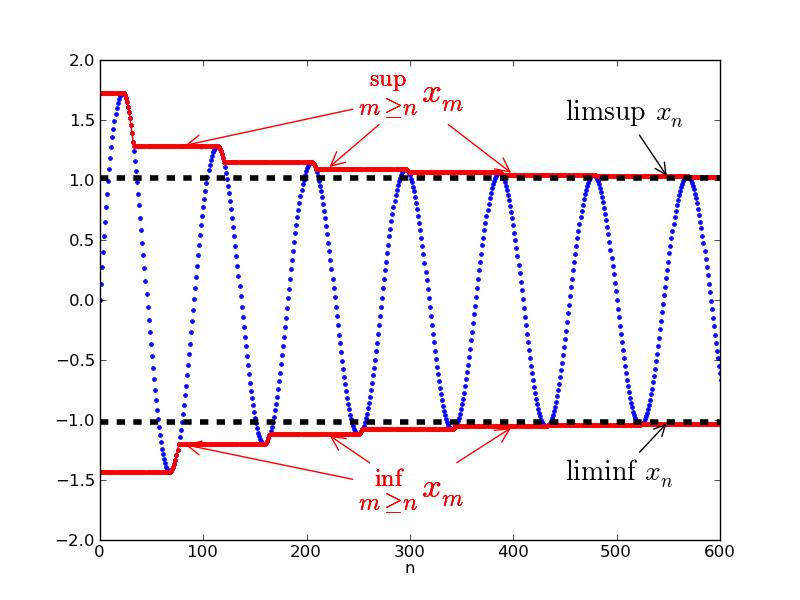
\includegraphics[width=\textwidth]{Lim_sup_example_5}
\begin{Definition}
	A number (or the symbol $ - \infty $ or $ +\infty $) is called a \textit{partial limit} of a sequence, if the sequence contains a subsequence converging to that number.
\end{Definition}

\begin{Proposition}
	The inferior and superior limits of any sequence are respectively the smallest and largest partial limits of the sequence.
\end{Proposition}
\begin{proof}
	Let's assume that this sequence is bounded. First consider the inferior limit $ i = \varliminf_{k \to \infty}x_k $. The sequence $ i_n = \inf_{k\geqslant n}x_k $ is nondecreasing. Using the definition of the greatest lower bound, we choose by induction numbers $ k_n \in \Natural $ such that $ k_n < k_{n+1} $ and $ i_{k_n} \leqslant x_{k_n} < i_{k_n}+\frac{1}{n} $ (Taking $ i_1 $ we find $ k_1 $; taking $ i_{k_1+1} $ we find $ k_2 $, etc.). Since $ \lim\limits_{n \to \infty}i_n = \lim\limits_{n \to \infty}(i_n+\frac{1}{n}) = i $, we have $ \lim\limits_{n \to \infty}x_{k_n}=i $. It is the smallest partial limit since for every $ \varepsilon>0 $ there exists $ n \in \Natural $ such that $ i-\varepsilon<i_n $, that is $ i-\varepsilon <i_n = \inf_{k\geqslant n}x_k \leqslant x_k $ for any $ k \geqslant n $. Now we have $ i-\varepsilon < x_k $ for $ k >n $ means that no partial limit of the sequence can be less than $ i - \varepsilon $. But $ \varepsilon >0 $ is arbitrary, and hence no partial limit can be less than $ i $. The proof for the superior limit is of course analogous. \newpara
	Now if the sequence is not bounded below(resp. above), one can select a subsequence of it tending to $ -\infty $ (resp. $ +\infty $). But then we also have $ \varliminf_{k \to \infty}x_k = -\infty $ (resp. $ \varlimsup_{k \to \infty}x_k = +\infty $). Finally, if $ \varlimsup_{k \to \infty}x_k = -\infty $ (resp. $ \varliminf_{k \to \infty}x_k = +\infty $), the sequence itself tends to $ -\infty $ (resp. $ +\infty $).
\end{proof}

\begin{Corollary}
	A sequence has a limit or tends to $ \pm \infty $ iff its inferior and superior limits are the same.
\end{Corollary}
\begin{proof}
	The cases when $ \varliminf_{k \to \infty}x_k = \varlimsup_{k \to \infty}x_k = \pm \infty $ have benn investigated above, and so we may assume that $ \varliminf_{k \to \infty}x_k = \varlimsup_{k \to \infty}x_k = A \in \Real $. Since $ (i_n = \inf_{k \geqslant n}x_k) \leqslant x_k \leqslant (\sup_{k \geqslant n}x_k = s_n) $, we have $ \lim\limits_{n \to \infty}x_n = A $.
\end{proof}

\begin{Corollary}
	A sequence converges iff every subsequence of it converges.
\end{Corollary}
\begin{proof}
	The inferior and superior limits of a subsequence lie between those of the sequence itself. If the sequence converges, then its subsequences must converge, and their limits are the same. The converse assertion is obvious, since the subsequence can be chosen as the sequence itself.
\end{proof}

\begin{Corollary}
	The Bolzano-Weierstrass Lemma in its restricted and wider formulations(corresponding to Lemmas at page 32 and page 33) follows from the Proposition we just proved.
\end{Corollary}
\begin{proof}
	If the sequence $ \{x_k\} $ is bounded, then $ i = \varliminf_{k \to \infty}x_k $ and $ s = \varlimsup_{k \to \infty}x_k $ are finite and partial limits of the sequence. When $ i=s $ some subsequences have a unique limit, and at least two when $ i<s $. If the sequence is unbounded on one side or the other, there exists a subsequence tending to the corresponding infinity.
\end{proof}



\subsection{Elementary Facts about Series}

\subsubsection{The Sum of a Series and the Cauchy Criterion for Convergence of Series}

\begin{Definition}
	The expression $ a_1 + a_2 + \cdots +a_n + \cdots$ is denoted by the symbol $ \sum_{n=1}^{\infty}a_n $ and usually called a \textit{series} or an \textit{infinite series}.
\end{Definition}

\begin{Definition}
	The elements of the sequence $ \{a_n\} $, when regarded as elements of the series, are called the \textit{terms} of the series. The element $ a_n $ is called the \textit{$ n $th term}.
\end{Definition}

\begin{Definition}
	The sum $ s_n = \sum_{k=1}^{n}a_k $ is called the \textit{partial sum of the series} or the \textit{$ n $th partial sum of the series}.
\end{Definition}

\begin{Definition}
	If the sequence $ \{s_n\} $ of partial sums of a series converges(resp. divergence), we say the series is \textit{convergent} (resp. \textit{divergent}).
\end{Definition}

\begin{Definition}
	The limit $ \lim\limits_{n \to \infty}s_n = s $ of the sequence of partial sums of the series, if it exists, is called the \textit{sum of the series}.
\end{Definition}
One can see that $ \sum_{n=1}^{\infty}a_n=s $.

\begin{Theorem}[The Cauchy convergence criterion for a series]
	The series $ a_1 + \cdots + a_n + \cdots $ converges iff for every $ \varepsilon >0 $ there exists $ N \in \Natural $ such that the inequalities $ m \geqslant n > N $ imply $ |a_n + \cdots +a_m|<\varepsilon $.
\end{Theorem}

\begin{Corollary}
	If only a finite number of terms of a series are changed, the resulting new series will converge if the original series did and diverge if it diverged.
\end{Corollary}

\begin{Corollary}
	A necessary condition for convergence of the series $ a_1 + \cdots + a_n + \cdots $ is that the terms tend to zero as $ n \to \infty $, that is, it is necessary that $ \lim\limits_{n \to \infty}a_n=0 $.
\end{Corollary}
\begin{proof}
	Set $ m=n $ in the Cauchy convergence criterion and use the definition of the limit of a sequence. \newpara
	Alternatively, $ a_n = s_n - s_{n-1} $, and, given that $ \lim\limits_{n \to \infty}s_n=s $, we have $ \lim\limits_{n \to \infty} a_n =  \lim\limits_{n \to \infty} (s_n - s_{n-1}) = s -s = 0$ .
\end{proof}

\begin{Example}
	The series $ 1+q+q^2+ \cdots + q^n + \cdots  $ is often called the \textit{geometric series}. It converges iff $ |q|<1 $.
\end{Example}
\begin{proof}
	Suppose $ |q|\geqslant 1 $, then we have $ |q^n| \geqslant 1 $, and in this case this series does not converges.\newpara
	Now let $ |q|<1 $, and we'll have $ s_n = 1+ q + \cdots + q^{n-1} = \frac{1-q^n}{1-q} $ and $ \lim\limits_{n \to \infty}s_n = \frac{1}{1-q} $, since $ \lim\limits_{n \to \infty}q^n = 0 $ if $ |q|<1 $.
\end{proof}

\begin{Example}
	The series $ 1+\frac{1}{2}+ \cdots +\frac{1}{n}+ \cdots$, called the \textit{harmonic series}, diverges because its partial sums $ s_n = 1+ \frac{1}{2}+\cdots \frac{1}{n} $ diverges.
\end{Example}
\begin{proof}
	It's sufficient to prove that its partial sum $ s_n = 1+ \frac{1}{2}+\cdots \frac{1}{n} $ diverges. For all $ n \in \Natural $ we have 
	\begin{equation}
		|x_{2n}-x_n| = \frac{1}{n+1}+ \cdots + \frac{1}{n+n} > n \cdot \frac{1}{2n} = \frac{1}{2}\nonumber
	\end{equation}
	and our proof completes.
\end{proof}

\textbf{\textit{Remark}} Usual laws for dealing with finite sums does not apply to series in general (e.g. insert parentheses to a divergent series). 

\subsubsection{Absolute Convergence. The Comparison Theorem and Its Consequences}

\begin{Definition}
	The series $ \sum_{n=1}^{\infty} $ is \textit{absolutely} convergent if the series $ \sum_{n=1}^{\infty}|a_n| $ converges.
\end{Definition}

Since $ |a_n + \cdots + a_m| \leqslant |a_n|+\cdots |a_m|$, the Cauchy convergence criterion implies that an absolutely convergent series converges, but the converse is generally not true.

\begin{Example}
	The series $ 1-1+\frac{1}{2}-\frac{1}{2}+ \frac{1}{3}-\frac{1}{3}+ \cdots$, whose partial sums are either $ \frac{1}{n} $ or $ 0 $, converges to $ 0 $. However, this sequence does not absolutely converges, and its proof is similar to the proof for the divergence of harmonic series.
\end{Example}

\begin{Theorem}[Criterion for convergence of series of non-negative terms]
	A series whose terms are non-negative converges iff the sequence of partial sums is bounded above.
\end{Theorem}

\begin{Theorem}[Comparison Theorem]
	Let $ \sum_{n=1}^{\infty}a_n $ and $ \sum_{n=1}^{\infty}b_n $ be two series with non-negative terms. If there exists an index $ N\in \Natural $ such that $ a_n \leqslant b_n $ for all $ n >N $, then the convergence of the series $  \sum_{n=1}^{\infty}b_n $ implies the convergence of $ \sum_{n=1}^{\infty}a_n $, and the divergence of $ \sum_{n=1}^{\infty}a_n $ implies the divergence of $\sum_{n=1}^{\infty}b_n $.
\end{Theorem}
\begin{proof}
	Omit terms for these two series for all $ n < N $, since a finite number of terms has no effect on the convergence of a series. Denote the partial sum of the sequences as $ A_n = \sum_{k=1}^{n}a_k \leqslant \sum_{k=1}^{n}b_k=B_n $. If the series $ \{B_n\} $ converges, then $ \{A_n\} $ is bounded above. Because $ \{A_n\} $ is also non-decreasing (all terms are non-negative), it has a limit, and so do $  \sum_{n=1}^{\infty}a_n  $. The second assertion is similar and can be proved by contradiction.
\end{proof}

\begin{Corollary}[The Weierstrass M-test for absolute convergence]
		Let $ \sum_{n=1}^{\infty}a_n $ and $ \sum_{n=1}^{\infty}b_n $ be series. Suppose there exists an index $ X $ such that $ |a_n| \leqslant b_n $ for all $ n > N $. Then a sufficient condition for absolute convergence of the series $ \sum_{n=1}^{\infty}a_n $ is that the series $ \sum_{n=1}^{\infty}b_n $ converge. \newpara
		It's often summarized as following: I\textbf{f the terms of a series are majorized (in absolute value) by the terms of a convergent numerical series, then the original series converges absolutely}.
\end{Corollary}
\begin{proof}
	By the comparison theorem the series $ \sum_{n=1}^{\infty}|a_n| $ will then converge, and that is what is meant by the absolute convergence of $ \sum_{n=1}^{\infty}a_n $.
\end{proof}

\begin{Corollary}[Cauchy's Test]
	Let $ \sum_{n=1}^{\infty}a_n $ be a given series and $ \alpha = \varlimsup_{n \to \infty} \sqrt[n]{|a_n|}$. Then the following are true:\\
	a) if $ \alpha <1 $, the series converges absolutely;\\
	b) if $ \alpha >1 $, the series diverges; \\
	c) there exist both absolutely convergent and divergent series for which $ \alpha = 1 $.
\end{Corollary}
\begin{proof}
	For $ \alpha>0 $, we find a $ q \in \Real $ such that $ \alpha <q<1 $, and show that the sequence $ \sum_{n=1}^{\infty}q^n $ converges and its terms are always greater than $ |a_n| $. Thus the original sequence absolutely converges. \newpara
	For $ \alpha>1 $, we find that $ \alpha $ is the greatest partial limit of the sequence $ \{\sqrt[n]{|a_n|}\} $. Hence for some $ k>K (|a_{n_k}|>1)  $, and the necessary condition for convergence ($ a_n \to 0 $) does not meet for the original sequence. \newpara
	If $ \alpha=1 $, for example, the series $ \sum_{n=1}^{\infty}\frac{1}{n} $ diverges and $ \sum_{n=1}^{\infty}\frac{1}{n^2} $ converges absolutely, but their superior limit under $ n $th root are both $ 1 $.
\end{proof}

\begin{Corollary}[d'Alembert's Test]
	Suppose the limit $ \lim\limits_{n \to \infty} |\frac{a_{n+1}}{a_n}|= \alpha $ exists for the series $ \sum_{n=1}^{\infty}a_n $. Then, \\
	a) if $ \alpha <1 $, the series converges absolutely;\\
	b) if $ \alpha >1 $, the series diverges; \\
	c) there exist both absolutely convergent and divergent series for which $ \alpha = 1 $.
\end{Corollary}

\begin{proof}
	If $ \alpha<1 $, then we find a number $ q $ such that $ \alpha < q <1 $. Fixing $ q $ and use the properties of limits, we find an index $ N \in \Natural$ such that $ |\frac{a_{n+1}}{a_n}|<q $ for $ n > N $. Since
	\begin{equation}
		|\frac{a_{n+1}}{a_n}|\cdot |\frac{a_n}{a_{n-1}}|\cdots |\frac{a_2}{a_1}| = \frac{a_{n+1}}{a_1}\nonumber
	\end{equation}
	and therefore we have $ |a_{n+1}|<|a_1|\cdot q^n $. But the geometric series $ \sum_{n=1}^{\infty}|a_1|q^n $ converges for $ |q|<1 $, hence the original series converges. \newpara
	For $ \alpha >1 $, we can find some terms that $ |\frac{a_{n+1}}{a_n}|>1 $, thus it diverges. For case involving $ \alpha=1 $, the examples from our proof for \textbf{Cauchy's Test} are sufficient.
\end{proof}

\begin{Proposition}[Cauchy]
	If $ a_1 \geqslant a_2 \geqslant \cdots \geqslant 0 $, the series $ \sum_{n=1}^{\infty}a_n $ converges iff the series $ \sum_{k=0}^{\infty}2^ka_{2^k} = a_1 + 2a_2 + 4a_4 + 8a_8 \cdots$ converges.
\end{Proposition}
\begin{proof}
	By the inequality
	\begin{equation}
		2^na_{2^{n+1}} \leqslant a_{2^n+1} + \cdots + a_{2^{n+1}} \leqslant 2^na_{2^n}
	\end{equation}
	we have 
	\begin{equation}
		\frac{1}{2}(S_{n+1}-a_1)\leqslant A_{2^{n+1}}-a_1 \leqslant S_n
	\end{equation}
	where $ A_k = a_1 + \cdots +a_k $ and $ S_n = a_1+2a_2+\cdots +2^n a_{2^n} $. $ \{A_k\} $ and $ \{S_n\} $ are non-decreasing, and hence they are both bounded above or unbounded above. Since all their terms are non-negative, our proof completes.
\end{proof}

\begin{Corollary}
	The series $ \sum_{n=1}^{\infty}\frac{1}{n^p} $ converges for $ p>1 $ and diverges for $ p \leqslant1 $.
\end{Corollary}
\begin{proof}
	If $ p \geqslant0 $, by our proposition it converges when $ 2^{1-p}<1 $, that is, $ p>1 $. The case when $ p \leqslant 0 $ is obvious since all terms are not smaller than 1.
\end{proof}


\subsubsection{The Number $ e $ as the Sum of a Series}
We know that $ e=\lim\limits_{n \to \infty}(1+\frac{1}{n})^n $. By Newton's binomial formula:
\begin{align}
	(1+\frac{1}{n})^n &= 1 + \frac{n}{1!}\frac{1}{n} + \frac{n(n-1)}{2!}\frac{1}{n^2} + \cdots + \frac{(n(n-1)\cdots(n-k+1))}{k!}\frac{1}{n^k}+ \cdots +\frac{1}{n^n} \\
	&= 1+ 1+ \frac{1}{2!}(1-\frac{1}{n}) + \cdots + \frac{1}{k!}(1-\frac{1}{n})(1-\frac{2}{n}) \times \cdots \\
	&\times (1-\frac{k-1}{n}) + \cdots + \frac{1}{n!}(1-\frac{1}{n})\cdots(1-\frac{n-1}{n})
\end{align}
Setting $ (1+\frac{1}{n})=e_n $ and $ 1+1+\cdots \frac{1}{2!} + \cdots + \frac{1}{n!}=s_n$, we thus have $\forall n \in \Natural(e_n < s_n)  $. \newpara
On the other hand, for any fixed $ k $ and $ n \geqslant k $, as can be seen from the same expansion, we have
\begin{equation}
	1+1+1+ 1+ \frac{1}{2!}(1-\frac{1}{n}) + \cdots + \frac{1}{k!}(1-\frac{1}{n})(1-\frac{2}{n})\cdots (1-\frac{k-1}{n})<e_n \nonumber
\end{equation}
As $ n \to \infty $ the left-hand side of the inequality tends to $ s_k $ and the right-hand side to $ e $. We can now conclude that $ s_k \leqslant e $ for all $ k \in \Natural $. Then from the relation $ e_n < s_n \leqslant e $ we find that $ \lim\limits_{n \to \infty}s_n=e $.
\begin{Definition}
	$ e=1+\frac{1}{1!}+ \frac{1}{2!}+\cdots+\frac{1}{n!}+\cdots $
\end{Definition}
The difference between $ e $ and its estimation $ s_n $ can be expressed as following
\begin{align}
	0<e-s_n &= \frac{1}{(n+1)!}+ \frac{1}{(n+2)!}+ \cdots =\\
	&= \frac{1}{(n+1)!}[1+\frac{1}{n+2}+\frac{1}{(n+2)(n+3)}+\cdots] < \\
	&< \frac{1}{(n+1)!}[1+\frac{1}{n+2}+\frac{1}{(n+2)^2}+\cdots] \\
	&=\frac{1}{(n+1)!}\frac{1}{1-\frac{1}{n+2}} = \frac{n+2}{n!(n+1)^2} < \frac{1}{n!n}
\end{align}
This estimate of the difference $ e-s_n $ can be written as the equality 
\begin{equation}
	e=s_n+\frac{\theta_n}{n!n} \nonumber
\end{equation}

where $ 0<\theta_n<1 $. \\

Hence $ e $ is irrational.
\begin{proof}[$ e $'s irrationality]
	Suppose the contrary, that $ e = \frac{p}{q} $, where $ p,q \in \Natural $. Then the number $ q!e $ must be an integer, while
	\begin{equation}
		q!e = q!(s_q+\frac{\theta_n}{q!q}) = q!+\frac{q!}{1!}+ \frac{q!}{2!}+\cdots+\frac{q!}{n!}+\frac{\theta_q}{q} \nonumber
	\end{equation}
	and therefore $ \frac{\theta_q}{q} $ would have to be an integer, which is impossible.
\end{proof}

Moreover, $ e $ is transcendental.





\section{The Limit of a Function}

\subsection{Definitions and Examples}

	Let $ E \subset \Real $, $ a $ be an limit point of $ E $, and $ f : E \to \Real $ be a real-valued function defined on $ E $.
\begin{Definition}
The function $ f : E \to \Real  $ \textit{tends to} $ A $ as $ x $ \textit{tends to} $ a $, or that $ A $ is the \textit{limit} of $ f $ as $ x $ \textit{tends to} $ a $, if for every $ \varepsilon>0 $ there exists $ \delta>0 $ such that $ |f(x)-A|<\varepsilon $ for every $ x \in E $ such that $ 0<|x-a|<\delta $.
\begin{equation}
	\forall \varepsilon >0 \exists \delta >0 \forall x \in E(0<|x-a|<\delta \Rightarrow |f(x)-A|<\varepsilon)\nonumber
\end{equation}
which is denoted as $ \lim\limits_{E \ni x \to a}f(x) = A $.
\end{Definition}

\begin{Example}
	\begin{equation}
		\lim\limits_{E \ni x \to 0}x\sin\frac{1}{x}=0\nonumber
	\end{equation}
	\begin{proof}
		Let $ \varepsilon=\delta $.
	\end{proof}
\end{Example}

\begin{Definition}
	A \textit{deleted neighborhood} of a point is a neighborhood of the point from which the point itself has been removed. \newpara
	If $ U(a) $ denotes a neighborhood of $ a $, the deleted neighborhood is denoted as $ \mathring{U}(a) $. \newpara
	The sets
	\begin{align}
		U_E(a) &\coloneqq E \cap U(a) \\
		\mathring{U}_E(a)&\coloneqq E \cap \mathring{U}(a)
	\end{align}
	will be called respectively a \textit{neighborhood of $ a $} in $ E $ and a \textit{deleted neighborhood of $ a $} in $ E $. \newpara
	if the temporarily-adopted cumbersome symbols $ \mathring{U}^\delta_E(a) $ and $ V^\varepsilon _\Real(A) $ denote the deleted $ \delta $-neighborhood of $ a $ in $ E $ and the $ \varepsilon $-neighborhood of $ A $ in $ \Real $, then the definition of the limit of a function can be rewritten as
	\begin{equation}
		(\lim\limits_{E \ni x \to a}f(x) = A ) \coloneqq \forall V^\varepsilon_\Real(A)\exists\mathring{U}^\delta_E(a)(f(\mathring{U}^\delta_E(a))\subset V^\varepsilon_\Real(A)) .\nonumber
	\end{equation}
	This expression says that $ A $ is the limit of the function $ f $ as $ x $ tends to $ a $ in the set $ E $ if for every $ \varepsilon $-neighborhood $ V^\varepsilon_\Real(A) $ of $ A $ there exists a deleted $ \delta $-neighborhood $ \mathring{U}^\delta_E(a) $ of $ a $ in $ E $ whose image $ f(\mathring{U}^\delta_E(a)) $ under the mapping $ f:E\to \Real $ is entirely contained in $  V^\varepsilon_\Real(A) $.
\end{Definition}
Since every neighborhood of a point on the real line contains a symmetric neighborhood (a $ \delta $-neighborhood) of the same point, the \textbf{final version of our definition for a limit} is:
\begin{Definition}
	\begin{equation}
			(\lim\limits_{E \ni x \to a}f(x) = A ) \coloneqq \forall V_\Real(A)\exists\mathring{U}_E(a)(f(\mathring{U}_E(a))\subset V_\Real(A)) .\nonumber
	\end{equation}
\end{Definition}

\begin{Example}
	The function \begin{equation}
	sgn x =	\begin{cases} 1 & \text{for } x >0\\
		 0 & \text{for } x=0\\
		 -1 & \text{for } x<0
		 \end{cases} \nonumber
	\end{equation}
	(read "signum x") has no limit as $ x \to 0 $.
\end{Example}
\begin{proof}
Apparently no number distinct from $ -1,0,1 $ can be the limit of the function.But no matter what $ \mathring{U}(0) $ we choose, some points of it does not belong to the $ \varepsilon $-neighborhood of $ A $ with $ \varepsilon=\frac{1}{2} $, since $  \mathring{U}(0)  $ contains both positive and negative points while $ V(A) $ can't contain both $ 1 $ and $ -1 $ at the same time.
\end{proof}
When the function $ f $ is defined on a whole deleted neighborhood of a point $ a\in \Real $, that is, when $ \mathring{U}_E(a)=\mathring{U}_\Real(a)=\mathring{U}(a) $, we adopt the expression $ x \to a $ instead of $ E \ni x \to a $.

\begin{Example}
	\begin{equation}
		\lim\limits_{x \to 0} |sgn(x)|=1\nonumber
	\end{equation}
\end{Example}
\begin{proof}
	\begin{equation}
		\forall V(1) (f(\mathring{U}(0))=1\in V(1)) \nonumber
	\end{equation}
\end{proof}

\begin{Example}
	\begin{equation}
		\lim\limits_{\Real_-\ni x \to 0} sgn(x)=-1, \quad 	\lim\limits_{\Real_+\ni x \to 0} sgn(x)=1 \nonumber
	\end{equation}
\end{Example}

\begin{Example}
	$ \lim\limits_{x \to 0}\sin \frac{1}{x} $ has no limit.
\end{Example}
\begin{proof}
	In any deleted neighborhood of 0 $ \mathring{U}(0) $ there are always points of the form $ \frac{1}{-\pi/2+2\pi n} $ and $  \frac{1}{\pi/2+2\pi n} $ which assume the values $ -1 $ and $ 1 $ respectively, but for $ \varepsilon<1 $ these two numbers can't both lie in the $ \varepsilon $-neighborhood. 
\end{proof}

\begin{Example}
	If 
	\begin{align}
		E_- &=\{x\in \Real | x = \frac{1}{-\pi/2+2\pi n}, n \in \Natural\} \\
		E_+ &=\{x\in \Real | x = \frac{1}{\pi/2+2\pi n}, n \in \Natural\}
	\end{align}
	then
	\begin{align}
		&\lim\limits_{E_-\ni x \to 0}\sin \frac{1}{x} = -1 \\
		&\lim\limits_{E_+\ni x \to 0}\sin \frac{1}{x} = 1
	\end{align}
\end{Example}
The next proposition, also called the statement of the equivalence of the Cauchy definition of a limit(in terms of neighborhoods) and the Heine definition(in terms of sequences), is:
\begin{Proposition}
	The relation $ \lim\limits_{E \ni x \to a}f(x) = A $ holds iff for every sequence $ \{x_n\} $ of points $ x_n \in E\setminus a $ converging to $ a $, the sequence $ \{f(x_n)\} $ converges to $ A $.
\end{Proposition}
\begin{proof}
	First, $ (\lim\limits_{E \ni x \to a}f(x)=A) \Rightarrow(\lim\limits_{n \to \infty}f(x_n)=A) $ is obvious. Now for the converse, if $ A $ is not the limit of $ f(x) $ as $ E \ni x \to a $, then there exists a neighborhood $ V(A) $ such that for any $ n \in \Natural $, there is a point $ x_n $ in the deleted $ \frac{1}{n} $-neighborhood of $ a $ in $ E $ such that $ f(x_n)\notin V(A) $. But this means that the sequence $ \{f(x_n)\} $ does not converge to $ A $.
\end{proof}













\subsection{Properties of the Limit of a Function}

\subsubsection{Properties of Deleted Neighborhood of a Limit Point of a Set }
\begin{Example}
	$ \mathring{U}_E(a)\neq \varnothing $, that is, the deleted neighborhood of the point in $ E $ is nonempty.
\end{Example}
\begin{Example}
	$ \forall \mathring{U}^\prime_E(a)\forall \mathring{U}^{\prime\prime}_E(a)\exists\mathring{U}_E(a)(\mathring{U}_E(a)\subset \mathring{U}^\prime_E(a) \cap \mathring{U}^{\prime\prime}_E(a)) $, that is, the intersection of any pair of deleted neighborhoods contains a deleted neighborhood.
\end{Example}

\subsubsection{General Properties of the Limit of a Function}
\begin{Definition}
	A function $ f : E \to \Real $ assuming only one value is called \textit{constant}. A function $ f : E \to \Real  $ is called \textit{ultimately constant} as $ E \ni x \to a $ if it is constant in some deleted neighborhood $ \mathring{U}_E(a) $, where $ a $ is a limit point of $ E $.
\end{Definition}
\begin{Definition}
	A function $ f : E \to \Real  $ is \textit{bounded, bounded above,} or \textit{bounded below} respectively if there is a number $ C \in \Real $ such that $ |f(x)|<C $, $ f(x)<C $, or $ C<f(x) $ for all $ x \in E $.
\end{Definition}

\begin{Theorem}
	\textbf{a)} ($ f : E \to \Real  $ is ultimately the constant $ A $ as $ E \ni x \to a) \Rightarrow  (\lim\limits_{E \ni x \to a}f(x)=A)$ . \newpara
	\textbf{b)} $ (\exists \lim\limits_{E \ni x \to a}f(x))\Rightarrow (f: E \to \Real\text{ is ultimately bounded as } E \ni x \to a )$. \newpara
	\textbf{c)} $ (\lim\limits_{E \ni x \to a}f(x)=A_1 )\land(\lim\limits_{E \ni x \to a}f(x)=A_2 )\Rightarrow (A_1=A_2)$.
\end{Theorem}
\begin{proof}
	The proof is similar to how we prove that a ultimately constant sequence converges and its limits is unique.
\end{proof}

\subsubsection{Passage to the Limit and Arithmetic Operations}
\begin{Definition}
	If two numerical-valued functions $ f: E \to \Real $ and $ g : E \to \Real $ have a common domain of definition $ E $, the \textit{sum, product}, and \textit{quotient} are respectively the functions defined on the same set by the following formulas
	\begin{align}
		(f+g)(x)&\coloneqq f(x) + g(x) \\
		(f \cdot g)(x)&\coloneqq f(x)\cdot g(x)\\
		(\frac{f}{g})(x) &\coloneqq \frac{f(x)}{g(x)}\text{ if }\forall x \in E (g(x) \neq 0)  \\
	\end{align}
\end{Definition}


\begin{Definition}
	A function $ f : E \to \Real $ is said to be \textit{infinitesimal} as $ E \ni x \to a $ if $ \lim\limits_{E \ni x \to a}f(x)=0 $.
\end{Definition}

\begin{Proposition}
	\textbf{a)} If $ \alpha : E \to \Real $ and $ \beta : E \to \Real $ are infinitesimal functions as $ E \ni x \to a $, then their sum $ \alpha + \beta: E \to \Real $ is also infinitesimal as $ E \ni x \to a $. \newpara
	\textbf{b)} If $ \alpha : E \to \Real $ and $ \beta : E \to \Real $ are infinitesimal functions as $ E \ni x \to a $, then their product $ \alpha \cdot \beta: E \to \Real $ is also infinitesimal as $ E \ni x \to a $. \newpara
	\textbf{c)}  If $ \alpha : E \to \Real $ is infinitesimal as $ E \ni x \to a $ and $ \beta : E \to \Real $ is ultimately bounded as $ E \ni x \to a $, then the product $ \alpha \cdot \beta: E \to \Real $ is infinitesimal as $ E \ni x \to a $.
\end{Proposition}
\begin{proof}
	For assertion \textbf{a)}, we set $ |\alpha(x)<\frac{\varepsilon}{2}| $. \\
	Assertion \textbf{b)} is a special case of assertion \textbf{c)}, since every function that has a limit is ultimately bounded. \\
	Let $ M $ bounds $ |\beta(x)| $, and set $ |\alpha(x)| < \frac{\varepsilon}{M} $ will help to prove assertion \textbf{c)}.
\end{proof}

\begin{Example}
	\begin{equation}
	(\lim\limits_{E \ni x \to a}f(x)=A) \Leftrightarrow (f(x)=A+\alpha(x)\land \lim\limits_{E \ni x \to a} \alpha(x)=0) \nonumber
	\end{equation}
\end{Example}
\begin{proof}
	This follows immediately from the definition of limit, by virtue which
	\begin{equation}
	\lim\limits_{E \ni x \to a}f(x)=A \Leftrightarrow \lim\limits_{E \ni x \to a}(f(x)-A)=0 \nonumber
	\end{equation}
\end{proof}

\begin{Theorem}
	Let $ f: E \to \Real $ and $ g : E \to \Real $ be two functions with a common domain of definition. If $ \lim\limits_{E \ni x \to a}f(x)=A $ and $  \lim\limits_{E \ni x \to a}g(x)=B  $, then
	\begin{align}
		&\lim\limits_{E \ni x \to a}(f+g)(x)= A+B \\
		&\lim\limits_{E \ni x \to a}(f \cdot g)(x)= A \cdot B\\
		&\lim\limits_{E \ni x \to a}(\frac{f}{g})(x) = \frac{A}{B}\text{ if }\forall x \in E (g(x) \neq 0\text{ and }B \neq 0)  \\
	\end{align}
\end{Theorem}
\begin{proof}
	These properties can be derived from the properties of the limit of sequences according to the proposition above. In order to complete the proof, one only need to convert "for some $ N \in \Natural $" to $ \mathring{U}_E(a) $.
\end{proof}
\begin{proof}[alternative proof with infinitesimal functions]
	Let $ f(x)= \alpha(x)$ and $ g(x)=\beta(x) $, where $ \alpha(x) $ and $ \beta(x) $ are infinitesimal functions. The first two assertions are obvious. For the quotient one, find the value of $ \frac{f(x)}{g(x)}-\frac{A}{B} $ after proving that $ \frac{1}{g(x)} $ is ultimately bounded as $ E \ni x \to a $.
\end{proof}

\subsubsection{Passage to the Limit and Inequalities}
\begin{Theorem}
	\textbf{a)} If the functions $ f : E \to \Real $ and $ g: E \to \Real $ are such that $ \lim\limits_{E \ni x \to a}f(x)=A $, and $ \lim\limits_{E \ni x \to a}g(x)=B $ and $ A <B $, then there exists a deleted neighborhood $ \mathring{U}_E(a) $ of $ a $ in $ E $ at each point of which $ f(x)<g(x) $. \newpara
	\textbf{b)} If the relations $ f(x) \leqslant g(x) \leqslant h(x) $ hold for the functions $ f : E \to \Real $, $ g: E \to \Real $ and $ h:E \to \Real $, and if $  \lim\limits_{E \ni x \to a}f(x)= \lim\limits_{E \ni x \to a}h(x)=C $, then the limit of $ g(x) $ exists as $ E \ni x \to a $, and $ \lim\limits_{E \ni x \to a}g(x)=C $.
\end{Theorem}
\begin{proof}
	\textbf{a)} Choose a number $ C $ such that $ A<C<B $. By definition of limit, we find deleted neighborhoods $ \mathring{U}^\prime_E(a) $ and $ \mathring{U}^{\prime\prime}_E(a)  $ such that $ |f(x)-A|<C-A $ for $ x \in \mathring{U}^\prime_E(a)  $ and $ |g(x)-B|<B-C$ for $ x \in  \mathring{U}^{\prime\prime}_E(a)$. Then at any point of a deleted neighborhood $ \mathring{U}_E(a) $ contained in $ \mathring{U}^\prime_E(a) \cup  \mathring{U}^{\prime\prime}_E(a)  $, we have 
	\begin{equation}
		f(x)<A+(C-A) =C = B-(B-C)<g(x) \nonumber
	\end{equation}
	\textbf{b)} This proof is similar.
\end{proof}

\begin{Corollary}
	Suppose $ \lim\limits_{E \ni x \to a}f(x)=A $ and $ \lim\limits_{E \ni x \to a}g(x)=B $ . Let $ \mathring{U}_E(a) $ be a deleted neighborhood of $ a $ in $ E $. \newpara
	\textbf{a)} If $ f(x) > g(x) $ for all $ x \in  \mathring{U}_E(a)$, then $ A \geqslant B $; \newpara
	\textbf{b)} $ f(x) \geqslant g(x) $ for all $ x \in  \mathring{U}_E(a)$, then $ A \geqslant B $; \newpara
	\textbf{c)} $ f(x) > B $ for all $ x \in  \mathring{U}_E(a)$, then $ A \geqslant B $; \newpara
	\textbf{d)} $ f(x) \geqslant B $ for all $ x \in  \mathring{U}_E(a)$, then $ A \geqslant B $.
\end{Corollary}
\begin{proof}
	Assertion a) and b) can be proved by contradiction and the theorem mentioned above. Set $ g(x) \equiv B $ and we prove assertion c) and d).
\end{proof}

\subsubsection{Two Important Examples}
\begin{Example}
	\begin{equation}
		\lim\limits_{x \to 0}\frac{\sin x}{x}=1 \nonumber
	\end{equation}
\end{Example}
\begin{proof}
	The geometric proof is sufficient with the following conditions:
	\begin{align}
		&|\sin x| \leqslant |x| \nonumber \\
		& 0\leqslant |\sin x| \leqslant |x| \Rightarrow (\lim\limits_{x \to 0} |\sin x| = 0) \nonumber
	\end{align}
\end{proof}

Now we define the exponential, logarithmic, and power functions using the theory of real numbers and limits.
\textbf{A)} \textit{The exponential function} \newpara
Let $ a>1 $ \\
$ 1^0 $ For $ n \in \Natural $ we define inductively $ a^1 \coloneqq a\text{ , } a^{n+1} \coloneqq a^n \cdot a $\newpara
$ 2^0 $ $ a^0 = 1 \text{ , } a^{-n}=\frac{1}{a^n} $ \newpara
$ 3^0 $ We define $ a = a^1 = (a^{1/n})^m $ and $ a^{m/n} \coloneqq (a^{1/n})^m $, Now we have defined $ a^r $ for $ r \in \Quoziente $. \newpara
$ 4^0 $ By induction, for $ x>0 $ and $ y>0 $ we have $ (x<y) \Leftrightarrow (x^n<y^n) $, and in particular, $ (x=y)\Leftrightarrow (x^n = y^n) $.\newpara
$ 5^0 $ $ a^{(mk)/(nk)} = a^{m/n} $ for $ k \in \Zahlen $ and $ a^{m_1/n_1}\cdot  a^{m_2/n_2}=a^{m_1/n_1+m_2/n_2} $\newpara
$ 6^0 $ $ (r_1<r_2)\Rightarrow (a^{r_1}<a^{r_2}) $ for any $ r_1,r_2\in\Quoziente $.\newpara
$ 7^0 $ For $ r^0 \in \Quoziente (\lim\limits_{\Quoziente \ni r \to r_0}a^r=a^{r_0})$.
\begin{proof}
	First we prove that $ a^p\to1 $ as $ \Quoziente \ni p \to 0 $ by use the inequality $ a^{-1/n}<a^p<a^{1/n} $. Then we choose $ \delta $ such that $ 1-\varepsilon a^{-r_0} <a^p < 1 + \varepsilon a^{-r_0}$ for $ |p|<\delta $. If now $ |r-r_0|<\delta $, we have $ a^{r_0}(1-\varepsilon a^{-r_0} )<a^{r_0}\cdot a^{r-r_0} < a^{r_0}(1 + \varepsilon a^{-r_0} )$, which says $ a^{r_0}- \varepsilon < a^r< a^{r_0}+ \varepsilon$.
\end{proof}
$ 8^0 $ Let $ x \in \Real $, $ s = \sup_{\Quoziente \ni r <x}a^r $, and $ i = \inf_{\Quoziente \ni r >x}a^r  $. We show that $ s=i $.
\begin{proof}
	\begin{equation}
		a^{r_1}\leqslant s \leqslant i \leqslant a^{r_2}\nonumber
	\end{equation}
	and for $ 0<|r_2-r_1|<\delta $ we have $ 0 \leqslant i-s \leqslant\varepsilon $.
\end{proof}
We now define $ a^x \coloneqq s = i $. \newpara
$ 9^0 $ $ a^x = \lim\limits_{\Quoziente \ni r \to x}a^r $.
\begin{proof}
	We find $ r^\prime <x $ such that $ s - \varepsilon < a^{r^\prime} \leqslant s = a^x $ and $ r^{\prime\prime}>x $ such that $ a^x = i \leqslant a^{r^{\prime\prime} }< i+ \varepsilon$. Then for all $ r \in \Quoziente $ in $ (r^{\prime},r^{\prime\prime}) $
	\begin{equation}
		a^x - \varepsilon < a^r < a^x + \varepsilon \nonumber
	\end{equation}
\end{proof}
$ 10^0 $ For $ x_1,x_2 \in \Real $ and $ a >1 $, $ (x_1<x_2)\Rightarrow (a^{x_1}<a^{x_2}) $.\newpara
$ 11^0 $ For any $ x_1,x_2 \in \Real $, $ a^{x_1}\cdot a^{x_2} = a^{x_1+x_2}$.\newpara
$ 12^0 $ $ \lim\limits_{x \to x_0}a^x = a^{x_0} $.
\begin{proof}
	The proof is similar with the proof for $ 7^0 $.
\end{proof}
$ 13^0 $ The range of values of the function $ x \mapsto a^x $ is the set $ \Real_+ $.
\begin{proof}
	The proof is similar with our first step for proving the irrationality of $ \sqrt{2} $.
\end{proof}
$ 14^0 $ We repeat the construction mentioned above for $ 0<a<1 $. In $ 6^0 $ and $ 10^0 $ we find that $ (x_1<x_2)\Rightarrow(a^{x_1}>a^{x_2}) $ where $ 0<a<1 $. \newpara

\begin{Definition}
	The mapping $ x \mapsto a^x $ is called the \textit{exponential} function with base $ a $. In the case $ a = e $, it's denoted with $ exp (x) $, but in general it's denoted with $ exp_a (x)$.
\end{Definition}
\textbf{B)} \textit{The logarithmic function} \\
The properties of the exponential function show that it's bijective. Hence it has an inverse.
\begin{Definition}
	The mapping inverse to $ exp_a:\Real \to \Real_+ $ is called the \textit{logarithm to base a ($ 0<a,a \neq 1 $)}, and is denoted 
	\begin{equation}
		\log_a:\Real_+ \to \Real \nonumber
	\end{equation}
	for base $ a=e $, the logarithm is called the \textit{natural logarithm} and is denoted $ \ln:\Real_+ \to \Real $.
\end{Definition}

By definition of the logarithm as the function inverse to the exponential function, we have 
\begin{align}
	\forall x \in \Real (\log_a(a^x)&=x) \nonumber \\
	\forall y \in \Real_+(a^{\log_a(y)}&=y) \nonumber 
\end{align}
$ 1^\prime $ $ \log_a a =1 $. \newpara
$ 2^\prime $ $ \log_a(y_1 \cdot y_2) = \log_a y_1+ \log_a y_2 $.\newpara
$ 3^\prime $ $ \log_a y \to \log_a y_0 $ as $ \Real_+ \ni y \to y_0 \in \Real_+ $.
\begin{proof}
	We verify that $ y_0a^{-\varepsilon} < y < y_0a^\varepsilon $ when $ a>1 $ and take their logarithms.
\end{proof}
$ 4^\prime $ $ (\log_a y_1<\log_a y_2) \Leftrightarrow (y_1<y_2)$ if $ a>1 $ and $ (\log_a y_1>\log_a y_2) \Leftrightarrow (y_1<y_2)$ if $ 0<a<1 $. \newpara
$ 5^\prime $ The range of values of the function $ \log_a : \Real_+ \to \Real $ is the set $ \Real $.\newpara
$ 6^\prime $ $ \log_a(b^\alpha) =\alpha \log_a b$ holds for any $ b >0 $ and any $ \alpha \in \Real $.
\begin{proof}
	First we verify that the equality holds in the following conditions: $ \alpha \in \Natural $, $ \alpha = -1 $, $ \alpha \in \Zahlen $, $ \alpha = \frac{1}{n} $ for $ n \in \Zahlen $, $ \alpha \in \Quoziente $, $ \log_a b^\alpha = \lim\limits_{\Quoziente \ni r \to \alpha}\log_a b^r = \lim\limits_{\Quoziente \ni r \to \alpha} r \log_a b = \alpha \log_a b $ where $ r \in \Quoziente $ and $ \log_a b^r = r \log_a b $, finally, $ (a^\alpha)^\beta = a^{\alpha \beta} $.
\end{proof}

\textbf{C)} \textit{The power function} \\
\begin{Definition}
	The function $ x \mapsto x^\alpha $ defined on the set $ \Real_+ $ is called a power function, and the number $ \alpha $ is called its \textit{exponent}.
	\begin{equation}
		x^\alpha = a^{\log_a(x^\alpha)}=a^{\alpha \log_a(x)}\nonumber
	\end{equation}
\end{Definition}






\subsection{The General Definition of the Limit of a Function(Limit over a Base)}
\subsubsection{Bases; Definition and Elementary Properties}
\begin{Definition}
	A set $ \mathcal{B} $ of subsets $ B \subset X $ of a set $ X $ is called a \textit{base} in $ X $ if the following conditions hold:
	$ B_1) $ $ \forall B \in \mathcal{B}(B \neq \varnothing) $. \\
	$ B_2) $ $ \forall B_1 \in \mathcal{B} \forall B_2 \in \mathcal{B} \exists B \in \mathcal{B}(B \subset B_1 \cap B_2) $.
	These two conditions are related to the two properties of deleted neighborhood we mentioned in the previous subsection. "Base" here is an abbreviation for what is called a "filter base".
\end{Definition}
\begin{tabular}{| m{6em} | m{4em} | m{8em} | m{12em} |}
	\hline
	Notation for the base  &Read  &Elements of the base &Definition of and notation for elements \\
	\hline
	$ x \to a $ & $ x $ tends to $ a $ &Deleted neighborhoods of $ a \in \Real $ &$ \mathring{U}(a)\coloneqq \{x \in \Real | a- \delta_1 < x <a+ \delta_2 \land x \neq a\} $, where $ \delta_1>0 $ and $ \delta_2>0 $. \\
	\hline
	$ x \to \infty $ &$ x $ tends to infinity &Neighborhoods of infinity & $ U(\infty)\coloneqq \{x \in \Real | \delta<|x|\} $, where $ \delta \in \Real $ \\
	\hline
	$ x \to a, x \in E $ or $ x \to_{\in E} a$ or $ E \ni x \to a $ &$ x $ tends to $ a $ in $ E $ & Deleted neighborhoods \footnotemark of $ a $ in $ E $ &$ \mathring{U}_E(a)\coloneqq E \cap \mathring{U}(a) $ \\
	\hline
	$ x \to \infty, x \in E $ or $ E \ni x \to \infty $ or $ x \to_{\in E} \infty $ &$ x $ tends to infinity in $ E $ &Neighborhoods\footnotemark of infinity in $ E $ &$ U_E(\infty)\coloneqq E \cap U(\infty) $ \\
	\hline
\end{tabular}
\footnotetext[1]{It is assumed that $ a $ is a limit point of $ E $}
\footnotetext[2]{It is assumed that $ E $ is not bounded}
\newline
If $ E = E^+_a=\{x \in \Real | x>a\} $(resp. $ E = E^-_a=\{x \in \Real | x<a\} $), we write $ x \to a + 0 $(resp. $ x \to a - 0 $), and we say that \textit{$ x $ tends to $ a $ from the right} (resp. \textit{$ x $ tends to $ a $ from the left}) or \textit{through larger values} (resp. \textit{through smaller values}). When $ a=0 $ we write $ x \to +0 $ (resp. $ x \to -0 $). \newpara
The notation $ E \ni x \to a +0 $ (resp. $ E \ni x \to a -0 $ ) will be used. It means that $ x $ tends to $ a $ in $ E $ while remaining larger (resp. smaller) than $ a $. \newpara
If
\begin{equation}
	E = E^+_\infty = \{x \in \Real | c<x\}\text{(resp.} E = E^-_\infty = \{x \in \Real | x<c\}\text{)} \nonumber
\end{equation}
we write $ x \to +\infty $ (resp. $ x \to - \infty $). When $ E = \Natural $, we shall write $ n \to \infty $ instead of $ x \to \infty, x \in \Natural $.\newpara

\subsubsection{The Limit of a Function over a Base}
\begin{Definition}
	Let $ f:X\to \Real $ be a function defined on a set $ X $ and $ \mathcal{B} $ a base in $ X $. A number $ A $ is called the \textit{limit of the function $ f $ over the base $ \mathcal{B} $} if for every neighborhood $ V(A) $ of $ A $ there is an element $ B \in \mathcal{B} $ whose image $ f(B) $ is contained in $ V(A) $.
	\begin{equation}
		(\lim\limits_{\mathcal{B}}f(x)=A )\coloneqq \forall V(A)\exists B\in \mathcal{B}(f(B)\subset V(A)\nonumber
	\end{equation}
\end{Definition}

\begin{Definition}
	A function $ f:X \to \Real $ is \textit{ultimately constant over the base $ \mathcal{B} $} if there exists a number $ A \in \Real $ and an element $ B\in \mathcal{B} $ such that $ f(x)=A $ for all $ x \in B $.
\end{Definition}
\begin{Definition}
	A function $ f:X \to \Real $ is \textit{ultimately bounded over the base $ \mathcal{B} $} if there exists a number $ c>0$ and an element $ B\in \mathcal{B} $ such that $ |f(x)| <c$ for all $ x \in B $.
\end{Definition}
\begin{Definition}
	A function $ f:X \to \Real $ is \textit{infinitesimal over the base $ \mathcal{B} $} if $ \lim\limits_{\mathcal{B}}f(x)=0 $.
\end{Definition}


\subsection{Existence of the Limit of a Function}
\subsubsection{The Cauchy Criterion}
\begin{Definition}
	The \textit{oscillation} of a function $ f:X \to \Real $ on a set $ E \subset X $ is
	\begin{equation}
		\omega(f,E) \coloneqq \sup_{x_1,x_2 \in E}|f(x_1)-f(x_2)|\nonumber
	\end{equation}
	that is, the least upper bound of the absolute value of the difference of the values of the function at two arbitrary points $ x_1,x_2 \in E $.
\end{Definition}

\begin{Theorem}[The Cauchy Criterion for the existence of a limit of a function]
	Let $ X $ be a set and $ \mathcal{B} $ a base in $ X $. \newpara
	A function $ f:X \to \Real $ has a \textit{limit over the base $ \mathcal{B} $} iff for every $ \varepsilon>0 $ there exists $ B \in \mathcal{B} $ such that the oscillation of $ f $ on $ B $ is less than $ \varepsilon $.
	\begin{equation}
		\exists \lim\limits_{\mathcal{B}}f(x) \Leftrightarrow \forall \varepsilon >0 \exists B \in \mathcal{B}(\omega(f,B)<\varepsilon) \nonumber
	\end{equation}
\end{Theorem}
\begin{proof}
	Setting $ m_B = inf_{x \in \mathcal{B}}f(x) $ and $ M_B = \sup_{x \in \mathcal{B}}f(x) $, and remarking that $ m_{B_1} \leqslant m_{B_1 \cap B_2} \leqslant M_{B_1 \cap B_2} \leqslant M_{B_2} $ for any elements $ B_1 $ and $ B_2 $ of the base $ \mathcal{B} $, we find by the axiom of completeness that there exists a number $ A \in \Real $ separating the numerical sets $ \{m_B\} $ and $ \{M_B\} $, where $ B \in \mathcal{B} $. Since $ \omega(f,B)=M_B-m_B $, we can now conclude that, since $ \omega(f,B) < \varepsilon $, we have $ |f(x)-A|<\varepsilon $ at every point $ x \in B $.
\end{proof}
\textbf{Remark:} When $ X = \Natural $ and $ \mathcal{B} $ is the base $ n \to \infty, n\in \Natural $, $ \omega(f, B) < \varepsilon $ where $ B \in \mathcal{B} $ is equivalent with the assertion that this sequence is a Cauchy sequence.



\subsubsection{The Limit of a Composite Function}
\begin{Theorem}[The Limit of a Composite Function]
	Let $ Y $ be a set, $ \mathcal{B}_Y $ a base in $ Y $, and $ g:Y \to \Real $ a mapping having a limit over the base $ \mathcal{B}_Y $. Let $ X $ be a set, $ \mathcal{B}_X $ a base in $ X $, and $ f:X \to Y $ a mapping of $ X $ into $ Y $ such that for every element $ B_Y \in \mathcal{B}_Y $ there exists $ B_X \in \mathcal{B}_X $ whose image $ f(B_X) $ is contained in $ B_Y $. \newpara
	Under these hypotheses, the composition $ g \circ f:X \to \Real $ of the mapping $ f $ and $ g $ is defined and has a limit over the base $ \mathcal{B}_X $ and $ \lim\limits_{\mathcal{B}_X}(g \circ f)(x) = \lim\limits_{\mathcal{B}_Y}g(y) $
\end{Theorem}
\begin{proof}
	Suppose $ \lim\limits_{\mathcal{B}_Y}g(y) = A $. $ g(B_Y) \subset V(A) \land (\exists B_X \in \mathcal{B}_X(f(B_X)\subset B_Y))\Rightarrow (g \circ f)(B_X) = g(f(B_X)) \subset g(B_Y) \subset V(A)$.
\end{proof}

\begin{Example}
	\begin{equation}
		\lim\limits_{x \to \infty} (1+ \frac{1}{x})^x = e \nonumber
	\end{equation}
\end{Example}
\begin{Example}
	\begin{equation}
		\lim\limits_{x \to +\infty} \frac{x}{q^x} = 0 \text{ if $ q>1 $} \nonumber
	\end{equation}
\end{Example}

\begin{Example}
	\begin{equation}
	\lim\limits_{x \to +\infty} \frac{\log_a x}{x}=0 \nonumber
	\end{equation}
\end{Example}


\subsubsection{The Limit of a Monotonic Function}
\begin{Theorem}[Criterion for the Existence of a Limit of a Monotonic Function]
	Assume $ i = \inf E $ and $ s = \sup E $ are limit points of the set $ E $ and  $ f : E \to \Real  $ a monotonic function on $ E $.A necessary and sufficient condition for this function that is non-decreasing on the set $ E $ to have a limit as $ x \to s, x \in E $, is that it be bounded above. For this function to have a limit as $ x \to i, x \in E $, it is necessary and sufficient that it be bounded below.
\end{Theorem}
\begin{proof}
	For $ x \to s $, use the definition of least upper bound and the fact the set $ \{x \in E|x_0 <x <s\} $ is an element of the base $ x \to s, x \in E $, where for a given $ \varepsilon >0 $ we have $ A- \varepsilon < f(x_0)\leqslant A $ and $ A = \sup_{x \in E\setminus \{s\}}f(x) $.
\end{proof}



\subsubsection{Comparison of the Asymptotic Behavior of Functions}

\begin{Definition}
	We shall say that a certain property of functions or a certain relation between functions holds \textit{ultimately over a given base $ \mathcal{B} $} is there exists $ B \in \mathcal{B} $ on which it holds.
\end{Definition}

\begin{Definition}
	The function $ f $ is said to be \textit{infinitesimal} compared with the function $ g $ over the base $ \mathcal{B} $, and we write $ f =_\mathcal{B} o(g) $ or $ f = o(g) $ over $ \mathcal{B} $ if the relation $ f(x) = \alpha(x)g(x) $ holds ultimately over $ \mathcal{B} $, where $ \alpha(x) $ is a function that is infinitesimal over $ \mathcal{B} $.
\end{Definition}

\begin{Definition}
	If $ f =_\mathcal{B} o(g) $ and $ g $ is itself infinitesimal over $ \mathcal{B} $, we say that $ f $ is an \textit{infinitesimal of higher order than $ g $ over $ \mathcal{B} $}.
\end{Definition}

\begin{Definition}
	A function that tends to infinity over a given base is said to be an \textit{infinite function} or simply an \textit{infinity} over the given base.
\end{Definition}

\begin{Definition}
	If $ f $ and $ g $ are infinite functions over $ \mathcal{B} $ and $ f =_\mathcal{B} o(g) $, we say that $ g $ is a \textit{higher order infinity} than $ f $ over $ \mathcal{B} $.
\end{Definition}

\begin{Example}
	\begin{equation}
	\lim\limits_{x \to +\infty}\frac{x^\alpha}{a^x}=0 \nonumber
	\end{equation}
	that is, $ x^\alpha = o(a^x) $ as $ x \to +\infty $ for $ a>1 $ and any $ \alpha \in \Real $.
\end{Example}

\begin{Example}
	\begin{equation}
		\lim\limits_{x \to +\infty}\frac{\log_a x}{x^\alpha} = 0\nonumber
	\end{equation}
	that is, for $ \alpha >0 $ we have $ \log_a x = o(x^\alpha) $ as $ x\to +\infty $.
\end{Example}

\begin{Definition}
	The notation $ f =_\mathcal{B} O(g) $ or $ f = O(g) $ over the base $ \mathcal{B} $ means that the relation $ f(x) = \beta(x)g(x) $ holds ultimately over $ \mathcal{B} $ where $ \beta(x) $ is ultimately bounded over $ \mathcal{B} $.
\end{Definition}

\begin{Definition}
	The functions $ f $ and $ g $ are \textit{of the same order over $ \mathcal{B} $}, and we write $ f\asymp g$ over $ \mathcal{B} $, if $ f =_\mathcal{B} O(g) $ and $ g =_\mathcal{B} O(f) $ simultaneously. This condition is equivalent to the condition that there exist $ c_1 > 0 $ and $ c_2>0 $ and an element $ B \in \mathcal{B} $ such that the relations
	\begin{equation}
		c_1|g(x)|\leqslant |f(x)|\leqslant c_2|g(x)|\nonumber
	\end{equation}
\end{Definition}

\begin{Example}
	The functions $ (2+\sin x)x $ and $ x $ are of the same order as $ x \to \infty $, but $ (1+ \sin x) $ and $ x $ are not of the same order as $ x \to \infty $.
\end{Example}

\begin{Definition}
	If the relation $ f(x) = \gamma(x) g(x) $ holds ultimately over $ \mathcal{B} $ where $ \lim\limits_{\mathcal{B}}\gamma(x)=1 $, we say that the function $ f $ \textit{behaves asymptotically like $ g $ over $ \mathcal{B} $}, or that $ f $ is \textit{equivalent to $ g $ over $ \mathcal{B} $}, and we write $ f \sim_\mathcal{B} g $ or $ f \sim g $ over $ \mathcal{B} $. This relation is indeed an equivalent relation.
\end{Definition}

\begin{Example}
	\begin{equation}
		\ln(1+x) \sim x\nonumber
	\end{equation}
	as $ x \to 0 $.
\end{Example}

\begin{Example}
	\begin{equation}
		e^x = 1 +x+o(x) \nonumber
	\end{equation}
	as $ x \to 0 $.
\end{Example}

\begin{Example}
	\begin{equation}
		(1+x)^\alpha = 1+ \alpha x + o(x) \nonumber
	\end{equation}
	as $ x \to 0 $.
\end{Example}

\begin{Proposition}
	If $ f \sim_\mathcal{B} \tilde{f} $, then $ \lim\limits_{\mathcal{B}}f(x)g(x)=  \lim\limits_{\mathcal{B}}\tilde{f}(x)g(x)$, provided one of these limits exists.
\end{Proposition}
This rule should not be extended to sums and differences of functions.

\begin{Proposition}
	For a given base \newpara
	\textbf{a)} $ o(f)+o(f)=o(f) $; \\
	\textbf{b)} $ o(f) $ is also $ O(f) $;\\
	\textbf{c)} $ o(f)+O(f)=O(f) $;\\
	\textbf{d)} $ O(f)+O(f)=O(f) $;\\
	\textbf{e)} if $ g(x) \neq0 $, then $ \frac{o(f(x))}{g(x)}=o(\frac{f(x)}{g(x)}) $ and $ \frac{O(f(x))}{g(x)} = O(\frac{f(x)}{g(x)}) $;\\
\end{Proposition}
Here the equality sign is used in the sense of "is". The symbols $ o(\cdot) $ and $ O(\cdot) $ do not really denoted a function, but rather indicate its asymptotic behavior, a behavior that many functions may have simultaneously.

\begin{align}
	e^x&= 1+\frac{1}{1!}x+\frac{1}{2!}x^2+\cdots+\frac{1}{n!}x^n+\cdots \text{ for $ x \in \Real $}\nonumber \\
	\cos x&= 1-\frac{1}{2!}x^2+\frac{1}{4!}x^4+\cdots+\frac{(-1)^k}{2k!}x^{2k}+\cdots \text{ for $ x \in \Real $}\nonumber \\
	\sin x&= \frac{1}{1!}x-\frac{1}{3!}x^3+\cdots+\frac{(-1)^k}{(2k+1)!}x^{2k+1}+\cdots \text{ for $ x \in \Real $} \nonumber \\
	\ln(1+x)&= x-\frac{1}{2}x^2+\frac{1}{3}x^3+\cdots+\frac{(-1)^{n-1}}{n}x^n + \cdots \text{ for $|x|<1 $}\nonumber \\
	(1+x)^\alpha&= 1+\frac{\alpha}{1!}x+\frac{\alpha(\alpha-1)}{2!}x^2+\cdots\\
	&\text{\quad}  +\frac{\alpha(\alpha-1)\cdots(\alpha-n+1)}{n!}x^n+\cdots \text{ for $|x|<1 $}\nonumber \\
\end{align}
And as $ x \to 0 $
\begin{align}
		e^x&= 1+\frac{1}{1!}x+\frac{1}{2!}x^2+\cdots+\frac{1}{n!}x^n+O(x^{n+1}) \nonumber \\
	\cos x&= 1-\frac{1}{2!}x^2+\frac{1}{4!}x^4-\cdots+\frac{(-1)^k}{2k!}x^{2k}+O(x^{2k+2}) \nonumber \\
	\sin x&= \frac{1}{1!}x-\frac{1}{3!}x^3+\cdots+\frac{(-1)^k}{(2k+1)!}x^{2k+1}+O(x^{2k+3})  \nonumber \\
	\ln(1+x)&= x-\frac{1}{2}x^2+\frac{1}{3}x^3-\cdots+\frac{(-1)^{n-1}}{n}x^n + O(x^{n+1})\nonumber \\
	(1+x)^\alpha&= 1+\frac{\alpha}{1!}x+\frac{\alpha(\alpha-1)}{2!}x^2+\cdots\\
	&\text{\quad}  +\frac{\alpha(\alpha-1)\cdots(\alpha-n+1)}{n!}x^n+O(x^{n+1}) \nonumber \\
\end{align}
These formulas can be derived from Taylor's formula, and they are usually the most efficient method of finding the limits of the elementary functions. When doing so, it is useful to keep in mind that $ O(x^{m+1}) = x^{m+1}\cdot O(1) = x^m \cdot x O(1)=x^m o(1) = o(x^m) $ as $ x \to 0 $.

\chapter{Continuous Functions}
\section{Basic Definitions and Examples}
\subsection{Continuity of a Function at a Point}
\begin{Definition}
	A real-valued function $ f $ is \textit{continuous at the point $ a $} if for any neighborhood $ V(f(a)) $ there is a neighborhood $ U(a) $ of $ a $ whose image under the mapping $ f $ is contained in $ V(f(a)) $.
	\begin{align}
	\text{$ f $ is continuous at $ a $} \coloneqq & (\forall V(f(a)))\exists U(a)(f(U(a))\subset V(f(a)))\nonumber \\
	&\forall \varepsilon >0 \exists U(a)\forall x \in U(a) (|f(x)-f(a)|<\varepsilon) \nonumber \\
	&\forall \varepsilon >0 \exists \delta>0 \forall x \in \Real (|x-a|<\delta \Rightarrow |f(x)-f(a|<\varepsilon) \nonumber
	\end{align}
\end{Definition}
This is equivalent to the condition that $ \lim\limits_{x \to a}f(x) $ exists and $ f(a) $ is defined.
\begin{equation}
	(f:E \to \Real \text{ is continuous at }a\in E)\Leftrightarrow(\exists \lim\limits_{\mathcal{B}_a}f(x))\nonumber
\end{equation}
where $ \mathcal{B}_a $ is the base consists of neighborhoods (not deleted neighborhoods) of $ a \in E $ .

\begin{Definition}[General Case]
	A function $ f:E \to \Real $ is \textit{continuous at the point $ a \in E $} if for every neighborhood $ V(f(a)) $ of the value $ f(a) $ that the function assumes at $ a $ there exists a neighborhood $ U_E(a) $ of $ a $ in $ E $ whose image $ f(U_E(a)) $ is contained in $ V(f(a)) $.
	\begin{align}
		&(f:E \to \Real \text{ is continuous at $ a\in E $ }) \coloneqq\\
		&(\forall V(f(a)))\exists U_E(a)(f(U_E(a))\subset V(f(a)))\nonumber \\
		&\forall \varepsilon >0 \exists U_E(a)\forall x \in U_E(a) (|f(x)-f(a)|<\varepsilon) \nonumber \\
		&\forall \varepsilon >0 \exists \delta>0 \forall x \in \Real (|x-a|<\delta \Rightarrow |f(x)-f(a|<\varepsilon \nonumber
	\end{align}
\end{Definition}

\begin{Definition}
	The quantity $ \omega(f,a) = \lim\limits_{\delta \to +0} \omega(f,U^\delta_E(a)) $ is called the \textit{oscillation} of $ f: E \to \Real $ at $ a $.
\end{Definition}
The oscillation of a function on a subset of a set does not exceed its oscillation on the set itself, so that $ \omega(f,U^\delta_E(a)) $ is a non-decreasing function of $ \delta $. 

\begin{equation}
(f:E \to \Real \text{ is continuous at }a\in E)\Leftrightarrow(\omega(f,a)=0)\nonumber
\end{equation}

\begin{Definition}
	A function $ f:E \to \Real $ is continuous on the set $ E $ if it is continuous at each point of $ E $.
\end{Definition}
The set of all continuous real-valued functions defined on a set $ E $ will be denoted $ C(E,\Real) $, or, more, $ C(E) $.
\begin{Example}
	The function $ f(x)=\sin x $ is continuous on $ \Real $.
\end{Example}
\begin{proof}
	For any point $ x_0 \in \Real $ we have
	\begin{align}
		|\sin x - \sin x_0|&=|2 \cos \frac{x+x_0}{2} \sin \frac{x- x_0}{2}| \nonumber\\
		&\leqslant 2|\sin\frac{x-x_0}{2}| \leqslant 2|\frac{x-x_0}{2}| = |x-x_0| < \varepsilon \nonumber
	\end{align}
	provided $ |x-x_0| < \delta = \varepsilon$. Here we used the inequality $ |\sin x| \leqslant |x| $.
\end{proof}

\begin{Example}
	Any sequence $ f: \Natural \to \Real $ is a function that is continuous on the set $ \Natural $ of natural numbers, since each point of $ \Natural $ is isolated.
\end{Example}

\subsection{Points of Discontinuity}
\begin{Definition}
	If the function $ f: E \to \Real $ is not continuous at a point of $ E $, this point is called a point of \textit{discontinuity} or simply a \textit{discontinuity} of $ f $.
\end{Definition}
\begin{Definition}
	If a point of discontinuity $ a \in E $ of the function $ f:E \to \Real $ is such that there exists a continuous function $ \tilde{f}:E \to \Real $ such that $ f|_{E \setminus a}=\tilde{f}|_{E \setminus a} $, then $ a $ is called a \textit{removable discontinuity} of the function $ f $.
\end{Definition}
\begin{Definition}
	The point $ a \in E $ is called a discontinuity of \textit{first kind} for the function $ f:E \to \Real $ if the following limits exist:
	\begin{equation}
	\lim\limits_{E \ni x \to a-0}f(x) \coloneqq f(a-0),\quad 	\lim\limits_{E \ni x \to a+0}f(x) \coloneqq f(a+0)\nonumber
	\end{equation}
	but at least one of them is not equal to $ f(a) $. If at least one of the two limits does not exist, then $ a $ is called a discontinuity of \textit{second kind}.
\end{Definition}

\begin{Example}
	The \textit{Dirichlet function}
	\begin{equation}
		\mathcal{D}(x)=\begin{cases}
		1&\text{ , if }x \in \Quoziente\\
		0&\text{ , if }x\in \Real \setminus \Quoziente
		\end{cases} \nonumber
	\end{equation}
	is discontinuous at every point, and obviously all of its discontinuities are of second kind, since in every interval there are both rational and irrational numbers.
\end{Example}
\begin{Example}
	The \textit{Riemann function}
	\begin{equation}
		\mathcal{R}(x)=\begin{cases}
		\frac{1}{n}&\text{ , if }x = \frac{m}{n} \in \Quoziente\text{ , where $ \frac{m}{n} $ is in lowest terms, }n \in \Natural\\
		0&\text{ , if }x\in \Real \setminus \Quoziente
		\end{cases} \nonumber
	\end{equation}
	is continuous at any irrational number. This function is discontinuous except for $ x=0 $, and all of these discontinuities are of first kind.
\end{Example}
\begin{proof}
	For any point $ a \in \Real $, any bounded neighborhood $ U(a) $ of it, and any number $ N \in \Natural $, $ U(a) $ contains only a finite number of rational numbers $ \frac{m}{n},m \in \Zahlen ,n\in\Natural$, with $ n<N $. \newpara
	By shrinking the neighborhood, one can then assume that the denominators of all rational numbers in the neighborhood (except possibly for the point $ a $ itself if $ a \in \Quoziente $) are larger than $ N $. Thus at any point $ x \in \mathring{U} (a)$ we have $ |\mathcal{R}(x)|< \frac{1}{N} $. Now we have shown that for any point $ a \in\Real\setminus\Quoziente $
	\begin{equation}
		\lim\limits_{x \to a}\mathcal{R}(x)=0 \nonumber
	\end{equation}
\end{proof}

\section{Properties of Continuous Functions}
\subsection{Local Properties}
\begin{Theorem}
	Let $ f:E \to \Real $ be a function that is continuous at the point $ a \in E $. Then the following statements hold: \newpara
	$ 1^0 $ The function $ f :E \to \Real $ is bounded in some neighborhood $ U_E(a) $. \\
	$ 2^0 $ If $ f(a)\neq 0 $, then in some neighborhood $ U_E(a) $ all the values of the function have the same sign as $ f(a) $.\\
	$ 3^0 $ If the function $ g:U_E(1)\to \Real $ is defined in some neighborhood of $ a $ and, like $ f $, is continuous at $ a $, then the following functions are defined in some neighborhood of $ a $ and continuous at $ a $:
	\begin{align}
		&\text{a) } (f+g)(x)\coloneqq f(x)+g(x) \\
		&\text{b) } (f \cdot g)(x)\coloneqq f(x )\cdot g(x)\\
		&\text{c) } \frac{f}{g}(x)\coloneqq \frac{f(x)}{g(x)}\text{ (provided $ g(a)\neq 0 $)}\\
	\end{align}
	$ 4^0 $ If the function $ g :Y \to \Real $ is continuous at a point $ b \in Y $ and $ f $ is such that $ f:E\to Y $, $ f(a)=b $, and $ f $ is continuous at $ a $, then the composite function $ (g \circ f)(x) $ is defined on $ E $ and continuous at $ a $.
\end{Theorem}
\begin{Example}
	All algebraic polynomials, rational functions, and the composition of a finite number of continuous functions are continuous at each point of its domain of definition.
\end{Example}



\subsection{Global Properties of Continuous Functions}

\begin{Theorem}[The Bolzano-Cauchy intermediate-value theorem]
	If a function that is continuous on a closed interval assumes values with different signs at the endpoints of the interval, then there is a point in the interval where it assumes the value $ 0$.
	\begin{equation}
		(f \in C[a,b]\land f(a) \cdot f(b)<0)\Rightarrow\exists c \in [a,b](f(c)=0) \nonumber
	\end{equation}
\end{Theorem}
\begin{proof}
	Divide the interval $ [a,b] $ in half where the point of division is the point that the function does not assume the value $ 0 $ and apply the nested interval lemma, then find the limit of the sequence of these two endpoints for the nested intervals.
\end{proof}

\begin{Corollary}
	If the function $ \varphi $ is continuous on an open interval and assumes values $ \varphi(a)=A $ and $ \varphi(b)=B $, then for any number $ C $ between $ A $ and $ B $, there is a point $ c $ between $ a $ and $ b $ at which $ \varphi(c)=C $.
\end{Corollary}

\begin{proof}
	The function $ f(x)=\varphi(x)-C $ is defined and continuous on the closed interval. The intermediate-value theorem implies that $ f(x) = \varphi(c)-C =0 $, since $ f(a)\cdot f(b)=(A-C)(B-C)<0 $.
\end{proof}

\begin{Theorem}[The Weierstrass maximum-value theorem]
	A function that is continuous on a closed interval is bounded on that interval. Moreover there is a point in the interval where the function assumes its maximum value and a point where it assumes its minimal value.
\end{Theorem}
\begin{proof}
	Let $ f:E \to \Real $ be a continuous function on the closed interval $ E =[a,b] $. By the local properties of a continuous function, for any point $ x \in E $ there exists a neighborhood $ U(x) $ such that the function is bounded on $ U_E(x) $. The set of such neighborhoods forms a covering of $ [a,b] $. By the finite covering lemma, one can extract a finite system of open intervals that cover $ [a,b] $. Since the function is bounded, one can find $ m_k \leqslant f(x)\leqslant M_k $ where $ x \in U_E(x_k) $.
	\begin{equation}
		min\{m_1,\cdots m_n\}\leqslant f(x) \leqslant max\{M_1,\cdots, M_N\} \nonumber
	\end{equation}
	Now let $ M = \sup_{x \in E}f(x) $. Set $ f(x) <M $ and contradiction arises by considering the auxiliary function $ \frac{1}{M-f(x)} $, which must be continuous by the local properties of $ f $, but also unbounded at the same time since $ M $ is the least upper bound and $ f(x) $ can be made arbitrarily close to $ M $ while $ f(x)-M $ does not assume zero. Similarly, one can prove that there exists a point such that $ f(x_m)=m $.
\end{proof}

\begin{Definition}
	If from every covering of a set by open intervals one can extract a finite subcovering, the set is called \textit{compact}. According to the  Heine–Borel theorem, in an Euclidean space, compact means that the set is closed (contains all of its limit points) and bounded (all of its points lie in some fixed distance).
\end{Definition}

\begin{Definition}
	A function $ f:E \to \Real $ is \textit{uniformly continuous} on a set $ E \subset \Real $ if for every $ \varepsilon>0 $ there exists $ \delta>0 $ such that $ |f(x_1)-f(x_2)|<\varepsilon $ for all points $ x_1,x_2 \in E $ such that $ |x_1-x_2|<\delta $. The following expression states the negation of the property of uniform continuity for a function:
	\begin{align}
		&(f:E \to \Real \text{ is not uniformly continuous } )\coloneqq \\
		&(\exists \varepsilon>0 \forall \delta>0 \exists x_1 \in E \exists x_2 \in E(|x_1-x_2|<\delta \land |f(x_1)-f(x_2)| \geqslant \varepsilon)) \nonumber
	\end{align}
\end{Definition}

\begin{Example}
	The function $ f(x) = x^2 $, which is continuous on $ \Real $, is not uniformly continuous on $ \Real $.
\end{Example}
\begin{proof}
	For all the points $ x_n^\prime = \sqrt{n+1} $ and $ x_n^{\prime\prime} =\sqrt{n}  $, where $ n \in \Natural $, $ f(x_n^\prime)-f(x_n^{\prime\prime}) = 1 $, but
	\begin{equation}
		\lim\limits_{n \to \infty}(\sqrt{n+1}-\sqrt{n}) = \lim\limits_{n \to \infty}\frac{1}{\sqrt{n+1}+\sqrt{n}} = 0 \nonumber
	\end{equation}
	so that for any $ \delta >0 $ there are points $ x_n^\prime  $ and $ x_n^{\prime\prime}  $ such that $ |x_n^\prime - x_n^{\prime\prime}|<\delta $, yet $ f(x_n^\prime)-f(x_n^{\prime\prime}) = 1 $.
\end{proof}

\begin{Example}
	The function $ f(x)=\sin(x^2) $, which is continuous and bounded on $ \Real $, is not uniformly continuous on $ \Real $.
\end{Example}

\begin{Theorem}[The Cantor-Heine Theorem on Uniform Continuity]
	A function that is continuous on a closed interval is uniformly continuous on that interval.
\end{Theorem}
\begin{proof}
	Let $ f:E \to \Real $ be a given function, $ E =[a,b] $, and $ f \in C(E) $. Since $ f $ is continuous at every point, we construct a system consists of $ \delta $-neighborhoods for all points $ x \in E $ such that the oscillation of that neighborhood is less than $ \varepsilon $. Let $ U(x)=U^{\delta(x)}(x) $ and $ V(x)=U^{\delta(x)/2}(x) $. Then the open intervals $ V(x),x \in E $ cover the closed interval $ [a,b] $. By the finite covering lemma we select a finite covering $ V(x_1),\cdots ,V(x_n)$. Let $ \delta=\{\frac{1}{2}\delta(x_1),\cdots,\frac{1}{2}\delta (x_n)\} $. Since this system of open intervals covers $ E $, there exists an interval $ V(x_i) $ that contains $ x^\prime $, and $ |x^\prime - x_i|<\frac{1}{2}\delta(x_i) $. But for another point $ x^{\prime\prime}\in E $ we have
	\begin{equation}
		|x^{\prime\prime}-x_i| \leqslant |x^\prime -x^{\prime\prime}|+|x^\prime-x_i| < \delta + \frac{1}{2}\delta(x_i) \leqslant \delta(x_i)\nonumber
	\end{equation}
	Consequently $ x^\prime,x^{\prime\prime} \in E $, and we have $ |f(x^\prime)-f(x^{\prime\prime})|\leqslant \omega(f,U^{\delta(x_i)}_E(x_i))<\varepsilon $.
\end{proof}

\begin{Proposition}
	A continuous mapping $ f:E \to \Real $ of a closed interval $ E=[a,b] $ into $ \Real $ is injective iff the function $ f $ is strictly monotonic on $ [a,b] $.
\end{Proposition}
\begin{proof}
	The fact that a strictly monotonic mapping is injective is obvious. For the converse, suppose the contrary, we find three points $ x_1<x_2<x_3 $ in the interval such that $ f(x_2) $ does not lie between $ f(x_1) $ and $ f(x_3) $. Let $ f(x_2)<f(x_1)<f(x_3) $. Since $ f $ is continuous, by Bolzano-Cauchy intermediate-value theorem, there exists a point $ x_1^\prime $ in $ [x_2,x_3] $ such that $ f(x_1^\prime)=f(x_1) $. We then have $ x_1<x_1^\prime $, but this contradicts to the injectiveness of this function.
\end{proof}

\begin{Proposition}
	Each strictly monotonic function $ f:X \to \Real $ defined on a numerical set $ X \subset \Real $ has an inverse $ f^{-1}:Y \to \Real $ defined on the set $ Y = f(X) $ of values of $ f $, and has the same kind of monotonicity on $ Y $ that $ f $ has on $ X $.
\end{Proposition}
\begin{proof}
	The mapping $ f:X \to Y $ is apparently both injective and surjective. Then $ \forall y_1 \in Y \forall y_2 \in Y (f^{-1}(y_1)<f^{-1}(y_2) \Leftrightarrow y_1 < y_2) $ if $ f $ is increasing on $ X $. The case when $ f $ is decreasing can be handled similarly.
\end{proof}

\begin{Proposition}
	The discontinuities of a function $ f:E \to \Real $ that is monotonic on the set $ E \subset \Real $ can be only discontinuities of first kind.
\end{Proposition}
\begin{proof}
	Let $ a $ be the point of discontinuity. It follows that $ a $ cannot be an isolated point of $ E $(some of its neighborhoods contain no points of $ E $ but $ a $ itself), since $ U_E(a)=a $ and $ f(U_E(a))=f(a)\subset V(f(a)) $ for any neighborhood of $ f(a) $. Then $ a $ must be a limit point of one of two following sets: $ E_a^- $ and $ E_a^+ $. Suppose $ f $ is non-decreasing, then the restriction $ f|_{ E_a^-} $ is a non-decreasing function that is bounded from above. Then the limit $ \lim\limits_{E_-\ni x \to a} f|_{ E_a^-}(x)=\lim\limits_{E \ni x \to a-0}f(x)=f(a-0)$ exists. The rest of this proof is analogous.
\end{proof}

\begin{Corollary}
	If $ a $ is a point of discontinuity of a monotonic function $ f:E \to \Real $, then at least one of the limits
	\begin{equation}
		\lim\limits_{E \ni x \to a-0}f(x)=f(a-0)\quad 	\lim\limits_{E \ni x \to a+0}f(x)=f(a+0) \nonumber
	\end{equation}
	exists, and strict inequality holds in at least one of the inequalities $ f(a-0) \leqslant f(a) \leqslant f(a+0) $ when $ f $ is non-decreasing and $ f(a-0) \geqslant f(a) \geqslant f(a+0)  $ when $ f $ is non-increasing. The function assumes no values in the open interval defined by the strict inequality. Open intervals of this kind determined by different points of discontinuity have no point in common.
\end{Corollary}
\begin{proof}
	The first assertion is obvious. For the second assertion, since $ f(x) \leqslant \lim\limits_{E \ni x \to a-0}f(x)=f(a-0) $ for $ x<a \in E $, the open interval $ (f(a-0),f(a) $ defined by the strict inequality $ f(a-0)<f(a) $ contains no value of this function. It's similar for $ f(a)<f(a+0) $. Let $ a_1 $ and $ a_2 $ be two different points of discontinuity of $ f $ and assume $ a_1<a_2 $. Since the function is non-decreasing
	\begin{equation}
		f(a_1-0)\leqslant f(a_1)\leqslant f(a_1+0)\leqslant f(a_2-0) \leqslant f(a_2) \leqslant f(a_2+0)\nonumber
	\end{equation}
	It follows from this that the intervals containing no values of $ f $ and corresponding to different points of discontinuity are disjoint.
\end{proof}


\begin{Corollary}
	The set of points of discontinuity of a monotonic function is at most countable.
\end{Corollary}
\begin{proof}
	The intervals are pairwise disjoint. Since they are defined by strict inequality, one can choose a rational number in each of these intervals,  so that the collection of intervals is equipollent with a subset of $ \Quoziente $.
\end{proof}

\begin{Proposition}[A Criterion for Continuity of a Monotonic Function]
	A monotonic function $ f:E \to \Real $ defined on a closed interval $ E = [a,b] $ is continuous iff its set of values $ f(E) $ is the closed interval with endpoints $ f(a) $ and $ f(b) $.
\end{Proposition}
\begin{proof}
	If $ f $ is a continuous monotonic function, its monotonicity implies that all the values $ f $ assumes on $ [a,b] $ lie between $ f(a) $ and $ f(b) $. Now we consider the converse. Suppose there is a point of discontinuity $ c $. Then one of the open intervals $ (f(c-0),f(c)) $ and $ (f(c),f(c+0)) $ contains no value of $ f $, but this interval is contained between $ f(a) $ and $ f(b) $ because of its monotonicity.
\end{proof}

\begin{Theorem}[The Inverse Function Theorem]
	A function $ f:X\to \Real $ that is strictly monotonic on a set $ X \subset \Real $ has an inverse $ f^{-1}:Y \to \Real $ defined on the set $ Y =f(X) $ of values of $ f $. The function $ f^{-1}:Y \to \Real $ is monotonic and has the same type of monotonicity on $ Y $ that $ f $ has on $ X $.
\end{Theorem}
\begin{proof}
	This can be easily proved with our last proposition.
\end{proof}


\chapter{Differential Calculus}
\section{Differentiable Functions}
\subsection{Functions Differentiable at a Point}
\begin{Definition}
	A function $ f:E \to \Real $ defined on a set $ E \subset \Real $ is \textit{differentiable} at a point $ a \in E $ that is a limit point of $ E $ if there exists a linear function $ A \cdot (x-a) $ of the increment $ x-a $ of the argument such that $ f(x)-f(a) $ can be represented as
	\begin{equation}
		f(x)-f(a) = A \cdot (x-a)+o(x-a) \text{ as }x\to a, x \in E \nonumber
	\end{equation}
	In other words, a function is differentiable at a point $ a $ if the change in its values in a neighborhood of the point in question is linear up to a correction that is infinitesimal compared with the magnitude of the displacement $ x-a $ from the point $ a $.
\end{Definition}

\begin{Definition}
	The linear function $ A \cdot (x-a) $ is called the \textit{differential} of the function $ f $ at $ a $. The differential of a function at a point is uniquely determined; for it follows from our former definition that 
	\begin{equation}
		\lim\limits_{E \ni x \to a}\frac{f(x)-f(a)}{x-a}=\lim\limits_{E \ni x \to a}(A+\frac{o(x-a)}{x-a}) =A\nonumber
	\end{equation}
	The uniqueness of $ A $ follows from the uniqueness of the limit.
\end{Definition}
\begin{Definition}
	The number
	\begin{equation}
			f^\prime(a)=\lim\limits_{E \ni x \to a}\frac{f(x)-f(a)}{x-a}\nonumber
	\end{equation}
	is called the \textit{derivative} of the function $ f $ at $ a $.
\end{Definition}
Differentiability of a function at a point is equivalent to the existence of its derivative at the same point.

\begin{Definition}
	A function $ f:E\to \Real $ defined on a set $ E \subset \Real $ is differentiable at a point $ x\in E $ that is a limit point of $ E $ if
	\begin{equation}
		f(x+h)-f(x)=A(x)h+\alpha(x,h) \nonumber
	\end{equation}
	where $ h \mapsto A(x)h $ is a linear function in $ f $ and $ \alpha(x,h) =o(h)$ as $ h \to 0, x+h \in E $. \newpara
	The quantities
	\begin{equation}
		\Delta x(h) \coloneqq (x+h)-x = h \nonumber
	\end{equation}
	and 
	\begin{equation}
		\Delta f (x,h) \coloneqq f(x+h) -f(x)\nonumber
	\end{equation}
	are called respectively the \textit{increment of the argument} and the \textit{increment of the function}.
\end{Definition}

\begin{Definition}
	The function $ h \mapsto A(x)h $, which is a linear in $ h $, is called the differential of the function $ f : E \to \Real $ at the point $ x \in E $ and is denoted $ d f(x)  $ or $ D f(x) $. Thus, $ d f(x)(h) = A(x)h $. From the definitions above we have
	\begin{equation}
		\Delta f(x,h) - d f(x)(h) = \alpha(x,h)\nonumber
	\end{equation}
	and $ \alpha(x,h) = o(h) $ as $ h \to 0,x+h \in E $. For this reason, we say that the differential is the \textit{(principal) linear part of the increment of the function}.
	\begin{equation}
		A(x) = f^\prime (x)=\lim\limits_{h \to 0, x+h,x \in E}\frac{f(x+h)-f(x)}{h} \nonumber
	\end{equation}
	The derivative is frequently denoted by the symbol $ \frac{d f(x)}{d x} $.
\end{Definition}




\subsection{The Tangent Line; Geometric Meaning of the Derivative and Differential}

\begin{Proposition}
	A function $ f:E \to \Real $ that is continuous at a point $ x_0 \in E $ that is a limit point of $ E \subset \Real $ admits a linear approximation iff it is differentiable at the point.
\end{Proposition}
\begin{Definition}
	If a function $ f:E \to \Real $ is defined on a set $ E \subset \Real $ and differentiable at a point $ x_0 \in E $, the line defined by $ y-f(x_0)=f^\prime(x_0)(x-x_0) $ that passing through $ (x_0,f(x_0)) $ and having slope $ f^\prime(x_0) $ is called the \textit{tangent} to the graph of this function at the point $ (x_0,f(x_0)) $.
\end{Definition}
\begin{Definition}
	If the mappings $ f : E \to \Real $ and $ g:E \to \Real $ are continuous at a point $ x_0 \in E $ that is a limit point of $ E $ and $ f(x)-g(x)=o((x-x_0)^n) $ as $ x \to x_0,x \in E $, we say that $ f $ and $ g $ have \textit{$ n $th order contact} at $ x_0 $ (more precisely, contact \textit{of order at least $ n $}). For $ n=1 $ we say that the mappings $ f $ and $ g $ are tangent to each other at $ x_0 $.
\end{Definition}

\subsection{Examples}
\begin{Example}
	If $ f(t)= r \cos \omega t $, then $ f^\prime(t) =- r \omega \sin \omega t$.
\end{Example}
\begin{proof}
	\begin{align}
		\lim\limits_{h \to 0} \frac{r \cos \omega (t+h)- r \cos \omega t}{h} &=r \lim\limits_{h \to 0}\frac{-2 \sin (\frac{\omega h}{2})\sin \omega (t+ \frac{h}{2})}{h} \\
		&= - r \omega \lim\limits_{h \to 0} \sin \omega (t+\frac{h}{2}) \cdot \lim\limits_{h \to 0}\frac{\sin (\frac{\omega h}{2})}{(\frac{\omega h}{2})} \\
		&= -r \omega \sin \omega t
	\end{align}
\end{proof}
\begin{Example}
	If $ f(t)=r \sin \omega t $, then $ f^\prime(t)=r \omega \cos \omega t $.
\end{Example}
\begin{proof}
	The proof is analogous.
\end{proof}
By the definition of differentiability of a function $ f:E \to \Real $ at a point $ x_0 \in E $, we have
\begin{equation}
	f(x)-f(x_0) = A(x_0)(x-x_0) + o(x-x_0) \text{ as } x\to x_0, x \in E \nonumber
\end{equation}
Since the right-hand side of this equality tends to zero as $ x \to x_0,x\in E $, it follows that $ \lim\limits_{E \ni x \to x_0} f(x)=f(x_0)$, so that a function that is differentiable at a point is necessarily continuous at that point. However, the converse is not always true. It's easy to see that although $ f(x)= |x| $ is continuous at $ 0 $, it's not differentiable at $ 0 $.
\begin{Example}
	$ e^{x+h}-e^x = e^x h + o(h) $ as $ h \to 0 $. Thus $ \frac{d e^x}{d x}=e^x $.
\end{Example}
\begin{proof}
	\begin{equation}
		e^{x+h}-e^x = e^x(e^h-1)=e^x(h+o(h)) = e^x h + o(h) \nonumber
	\end{equation}
	Here we have used the formula $ e^h -1 = h+ o(h)$ obtained in Section 3.2.4.
\end{proof}
\begin{Example}
	If $ a>0 $, then $ a^{x+h}-a^x=a^h(\ln a)h + o(h) $ as $ h \to 0 $. Thus $ d a^x = a^x (\ln a)d x $.
\end{Example}
\begin{proof}
	\begin{align}
		a^{x+h}-a^x&=a^x(a^h-1)=a^x(e^{h \ln a}-1)\\
		&=a^x(h \ln a+ o(h \ln a)) = a^x(\ln a) h + o(h) \text{ as } h \to 0
	\end{align}
\end{proof}

\begin{Example}
	If $ x \neq 0 $, then $ \ln|x+h|-\ln |x| = \frac{1}{x}h+o(h) $ as $ h \to 0 $. Thus $ d \ln |x| = \frac{1}{x}d x $.
\end{Example}
\begin{proof}
	\begin{equation}
	\ln|x+h|-\ln |x| = \ln|1+\frac{h}{x}|	\nonumber
	\end{equation}
	For $ |h|<|x| $ we have $ |1+\frac{h}{x}| = 1+ \frac{h}{x} $, and so for sufficiently small value of $ h $ we can write
	\begin{equation}
		\ln|x+h| - \ln |x| = \ln (a+\frac{h}{x}) = \frac{h}{x} + o(\frac{h}{x}) = \frac{1}{x}h + o(h) \nonumber
	\end{equation}
	as $ h \to 0 $. Here we have used the relation $ \ln(1+t) = t+o(t) $ as $ t \to 0 $, shown in Section 3.2.4.
\end{proof}

\begin{Example}
	If $ x \neq 0 $ and $ 0<a \neq 1 $, then $ \log_a|x+h| - \log_a|x| = \frac{1}{x \ln a}h + o(h) $ as $ h \to 0 $. Thus, $ d \log_a|x| = \frac{1}{x \ln a}d x $.
\end{Example}
\begin{proof}
	\begin{align}
		\log_a|x+h| - \log_a|x| &= \log_a |1 + \frac{h}{x}| = \log_a(1+ \frac{h}{x}) \\
		&= \frac{1}{\ln a} \ln(1+\frac{h}{x}) = \frac{1}{\ln a}(\frac{h}{x}+o(\frac{h}{x})) = \frac{1}{x \ln a}h + o(h)
	\end{align}
\end{proof}

\begin{Example}[Waerden's Function]
	Set
	\begin{equation}
		\Psi_0(x)=\begin{cases}
		&x,\quad \text{ if }0 \leqslant x \leqslant \frac{1}{2}\\
		&1-x, \quad \text{ if }\frac{1}{2}\leqslant x \leqslant 1
		\end{cases} \nonumber
	\end{equation}
	and extend this function to the entire real line so as to have period $ 1 $. We denote the extended function by $ \varphi_0 $. Further, let
	\begin{equation}
		\varphi_n(x)=\frac{1}{4^n}\varphi_0(4^n x)\nonumber
	\end{equation}
	The function $ \varphi_n $ has period $ 4^{-n} $ and a derivative equal to $ +1 $ or $ -1 $ everywhere except at the points $ x= \frac{k}{2^{2n+1}},k \in \Zahlen $. Let
	\begin{equation}
		f(x)=\sum_{n=1}^{\infty}\varphi_n(x) \nonumber
	\end{equation}
	This function is defined and continuous on $ \Real $, but does not have a derivative at any point.
\end{Example}
\begin{proof}
	The function series $ \{\varphi_n(x)\} $ is convergent by Weierstrass's M-test, thus the function is continuous everywhere. Now we prove that this function is not differentiable everywhere. \newpara
	For any positive $ n $ and any arbitrary point $ a $, choose $ h_n $ to be $ \frac{1}{4^{n+1}} $ or $ -\frac{1}{4^{n+1}} $, so that $ |\varphi_n(a+h_n)-\varphi_n(a)|=|h_n| $. This is possible because $ h_n $ is a quarter of the period of $ \varphi_n(x) $ and $ \varphi_n(x) $ is a linear function that has a slope of $ \pm 1 $ in the interval $ 2h_n $ containing $ a $. \newpara
	We can also see that for $ m \leqslant n $ we have $ |\varphi_m(a+h_n)-\varphi_m(a)|=h_n $ and for $ m>n$ we have $ |\varphi_m(a+h_n)-\varphi_m(a)|=0 $, since $ h_n $ can be expressed as $ \frac{4(m-n)}{4^{m}}$, a multiple of the period of $ \varphi_m(x) $. Hence $ \frac{f(a+h_n)-f(a)}{h_n} $ is an integer whose parity (the fact of being odd or even) is the same as $ n $. Therefore the limit $ \lim\limits_{n \to \infty}\frac{f(a+h_n)-f(a)}{h_n} $ cannot exist, which implies that this function is not differentiable at any arbitrary point.
\end{proof}



\section{The Basic Rules of Differentiation}
\subsection{Differentiation and the Arithmetic Operations}
\begin{Theorem}
	If two functions $ f $ and $ g $ are differentiable at $ x $, then their sum, product, and quotient if the denominator is not zero, are differentiable.
	\begin{align}
		(f+g)^\prime(x)&=(f^\prime+g^\prime)(x) \\
		(f\cdot g)^\prime(x)&=f^\prime(x)\cdot g(x) + f(x)\cdot g^\prime(x)\\
		(\frac{f}{g})^\prime (x) &=\frac{f^\prime(x)\cdot g(x) - f(x)\cdot g^\prime(x)}{g^2(x)}
	\end{align}
\end{Theorem}
\begin{proof}
	The theorem is easy to prove with the definition of a differentiable function and the properties of the symbol $ o(\cdot) $.
\end{proof}
\begin{Corollary}
	The derivative of a linear combination of differentiable functions equals the same linear combination of the derivatives of these functions.
\end{Corollary}
\begin{Corollary}
	If the function $ f_1 ,\cdots, f_n $ are differentiable at $ x $, then
	\begin{align}
		(f_1 \cdots f_n)^\prime(x)=&f^\prime_1(x)f_2(x)\cdots f_n(x)\\
		&f_1(x)f^\prime_2(x)f_3(x)\cdots f_n(x)+ \cdots f_1(x)\cdots f_{n-1}(x)f^\prime_n(x)
	\end{align}
\end{Corollary}
\begin{proof}
	Easy to prove by induction.
\end{proof}
\begin{Corollary}
	Following from the relation between the derivative and the differential, the theorem can also be written in terms of differentials.
\end{Corollary}


\subsection{Differentiation of a Composite Function(Chain Rule)}
\begin{Theorem}
	If the function $ f:X \to Y \subset \Real $ is differentiable at a point $ x \in X $ and the function $ g:Y \to \Real $ is differentiable at the point $ y=f(x)\in Y $, then the composite function $ g \circ f:X \to \Real $ is differentiable at $ x $, and the differential $ d(g \circ f)(x): T \Real(x) \to T \Real(g(f(x))) $ of their composition equals the composition $ d f(y)\circ d f(x) $ of their differentials
	\begin{equation}
		d f(x) :T \Real(x) \to T \Real(y=f(x)) \text{ and } d g(y=f(x)) : T \Real(y) \to T \Real(g(y)) \nonumber
	\end{equation}
\end{Theorem}
\begin{Corollary}
	The derivative $ (g \circ f)^\prime(x) $ of the composition of differentiable real-valued functions equals the product $ g^\prime(f(x))\cdot f^\prime(x) $ of the derivatives of these functions compared at the corresponding points.
\end{Corollary}
\begin{Corollary}
	If the composition $ (f_n \circ \cdots \circ f_1)(x) $ of differentiable functions $ y_1 = f_1(x),\cdots,y_n=f_n(y_n-1) $ exists, then
	\begin{equation}
		(f_n \circ \cdots \circ f_1)^\prime(x) = f^\prime_n(y_n-1)f^\prime_{n-1}(y_n-2) \cdots f^\prime_1(x) \nonumber
	\end{equation}
\end{Corollary}
\begin{Example}
	The derivative of the logarithm of the absolute value of a differentiable function is often called its \textit{logarithmic derivative}. \\
	Since $ F(x)=\ln |f(x)| = (\ln \circ || \circ f)(x) $, we have $ F^\prime(x) = (\ln |f|)^\prime (x)=\frac{f^\prime(x)}{f(x)} $
\end{Example}
\begin{Example}
	For a function $ u(x)^{v(x)} $, where $ u(x) $ and $ v(x) $ are differentiable functions and $ u(x)>0 $. We write $ u(x)^{v(x)} = e^{v(x)\ln u(x)} $, then
	\begin{equation}
		\frac{d e^{v(x)\ln u(x)}}{dx} = u(x)^{v(x)}\cdot v^\prime(x) \ln u(x) + v(x)u(x)^{v(x)-1}\cdot u^\prime(x) \nonumber
	\end{equation}
\end{Example}


\subsection{Differentiation of an Inverse Function}
\begin{Theorem}[The derivative of an inverse function]
	Let the functions $ f : X \to Y $ and $ f^{-1}:Y \to X $ be mutually inverse and continuous at points $ x_0 \in X $ and $ f(x_0)=y_0 \in Y $ respectively. If $ f $ is differentiable at $ x_0 $ and $ f^\prime(x_0)\neq 0 $, then $ f^{-1} $ is also differentiable at the point $ y_0 $, and
	\begin{equation}
		(f^{-1})^\prime(y_0)=(f^\prime(x_0))^{-1}\nonumber
	\end{equation}
\end{Theorem}
\begin{Example}
	The \textit{hyperbolic} and \textit{inverse hyperbolic functions} and their derivatives are:
	\begin{align}
		\sinh x &= \frac{1}{2}(e^x-e^{-x}) \\
		\sinh^\prime x &= \cosh x \\
		\arsinh y &= \ln(y+\sqrt{1+y^2})\\
		\arsinh^\prime y &= \frac{1}{\sqrt{1+y^2}}\\
		\cosh x &= \frac{1}{2}(e^x+e^{-x}) \\
		\cosh^\prime x &= \sinh x \\
		\arcosh_{-} y &= \ln (y-\sqrt{y^2-1})\\
		\arcosh_{+} y &= \ln (y+\sqrt{y^2-1})\\
		\arcosh^\prime_{-} y &=- \frac{1}{\sqrt{y^2-1}}, \quad y>1 \\
		\arcosh^\prime_{+} y &= \frac{1}{\sqrt{y^2-1}}, \quad y>1 \\		
		\tanh x &= \frac{\sinh x}{\cosh x} \\
		\tanh^\prime x &= \frac{1}{\cosh^2 x}\\
		\artanh y &= \frac{1}{2} \ln \frac{1+y}{1-y},\quad |y|<1 \\
		\artanh^\prime y &= \frac{1}{1-y^2}, \quad |y|<1\\
		\coth x &= \frac{\cosh x}{\sinh x} \\
		\coth^\prime x &= -\frac{1}{\sinh^2 x}\\
		\arcoth y &= \frac{1}{2} \ln \frac{y+1}{y-1},\quad |y|>1 \\
		\arcoth^\prime y &= -\frac{1}{y^2-1}, \quad |y|>1
	\end{align}
\end{Example}


\subsection{Higher-Order Derivatives}
\begin{Definition}
	The \textit{derivative of order $ n $} is defined by the formula 
	\begin{equation}
		f^{(n)}(x) \coloneqq (f^{(n-1)})^\prime(x)\nonumber
	\end{equation}
	The set of functions $ f:E \to \Real $ having continuous derivatives up to order $ n $ inclusive will be denoted $ C^{(n)}(E,\Real) $ or $ C^{(n)}(E)  $. $ C^{(0)}(E)=C(E) $ by $ f^{(0)}(x)=f(x) $.
\end{Definition}
\begin{Example}[Leibniz's formula]
	Let $ u(x) $ and $ v(x) $ be functions having derivatives up to order $ n $ inclusive on a common set $ E $. Then following formula of Leibniz holds for the $ n $th derivative of their product:
	\begin{equation}
		(uv)^{(n)} = \sum_{m=0}^{n}\binom{n}{m}u^{(n-m)}v^{(m)} \nonumber
	\end{equation}
\end{Example}


\section{The Basic Theorems of Differential Calculus}
\subsection{Fermat's Lemma and Rolle's Theorem}
\begin{Definition}
	A point $ x_0 \in E \subset \Real $ is called a \textit{local maximum} (resp. \textit{local minimum}) and the value of a function $ f:E \to \Real $ at the point a \textit{local maximum value} (resp. \textit{local minimum value}) if their exists a neighborhood $ U_E(x_0) $ of $ x_0 $ in $ E $ such that at any point $ x \in U_E(x_0) $ we have $ f(x)\leqslant f(x_0) $ (resp. $ f(x)\geqslant f(x_0) $).
\end{Definition}
\begin{Definition}
	If the strict inequality $ f(x)<f(x_0) $ (resp. $ f(x)>f(x_0) $) hods at every point $ x \in \mathring{U}_E(x_0) $, the point $ x_0 $ is called \textit{strict local maximum} (resp. \textit{strict local minimum}) and the value of the function $ f:E \to \Real $ a \textit{strict local maximum value} (resp. \textit{strict local minimum value}).
\end{Definition}
\begin{Definition}
	The local maxima and minima are called \textit{local extrema} and the values of the function at these points \textit{local extreme values of the function}.
\end{Definition}
\begin{Definition}
	An extremum $ x_0 \in E $ of the function $ f:E \to \Real $ is called an \textit{interior} extremum if $ x_0 $ is a limit point of both sets $ E_- = \{x\in E | x< x_0 \} $ and $ E_+ = \{x\in E | x> x_0 \}  $.
\end{Definition}
\begin{Lemma}[Fermat]
	If a function $ f:E \to \Real $ is differentiable at an interior extremum, $ x_0 \in E $, then its derivative at $ x_0 $ is $ 0 : f^\prime(x_0)=0 $.
\end{Lemma}
\begin{Proposition}[Rolle's Theorem]
	If a function $ f:[a,b] \to \Real $ is continuous on the closed interval $ [a,b] $ and differentiable on $ (a,b) $ and $ f(a)=f(b) $, then there exists a point $ \xi \in (a,b) $ such that $ f^\prime(\xi)=0 $.
\end{Proposition}


\subsection{The Theorems of Lagrange and Cauchy on Finite Increments}
\begin{Theorem}[Lagrange's Finite-increment Theorem]
	If a function $ f:[a,b]\to \Real $ is continuous on a closed interval $ [a,b] $ and differentiable on the open interval $ (a,b) $, there exists a point $ \xi \in [a,b] $ such that
	\begin{equation}
		f(b)-f(a)=f^\prime(\xi)(b-a) \nonumber
	\end{equation}
\end{Theorem}
\begin{proof}
	Consider the auxiliary function
	\begin{equation}
		F(x)=f(x)-\frac{f(b)-f(a)}{b-a}(x-a) \nonumber
	\end{equation}
	and apply Rolle's theorem to it.
\end{proof}
Note that this is valid only for numerical-valued functions.

\subsubsection{Corollaries of Lagrange's Theorem}
\begin{Corollary}[Criterion for monotonicity of a function]
	If the derivative of a function is nonnegative (resp. positive) at every point of an open interval, then the function is nondecreasing (resp. increasing) on that interval.
\end{Corollary}
An analogous assertion can be made about the nonincreasing (resp. decreasing) nature of a function with a nonpositive (resp. negative) derivative.
\begin{Corollary}[Criterion for a function to be constant]
	A function that is continuous on a closed interval is constant on it iff its derivative equals zero at every point of the interval $ [a,b] $ (or only on $ (a,b) $).
\end{Corollary}
If the derivative of two functions are equal on some interval, then the difference between them is constant.
\begin{Proposition}[Cauchy's Finite-increment Theorem]
	Let $ x=x(t) $ and $ y=y(t) $ be functions that are continuous on a closed interval $ [\alpha, \beta] $ and differentiable on the open interval $ (\alpha,\beta) $. \\
	Then there exists a point $ \tau \in [\alpha,\beta] $ such that
	\begin{equation}
		x^\prime(\tau)(y(\beta)-y(\alpha)) = y^\prime(\tau)(x(\beta)-x(\alpha))\nonumber
	\end{equation}
	If in addition $ x^\prime(t)\neq 0 $ for each $ t $ in $ (\alpha,\beta) $, then $ x(\alpha)\neq x(\beta) $ and we have the equality
	\begin{equation}
		\frac{y(\beta)-y(\alpha)}{x(\beta)-x(\alpha)} = \frac{y^\prime(\tau)}{x^\prime(\tau)} \nonumber
	\end{equation}
\end{Proposition}
\begin{proof}
	Consider the function $ F(t)=x(t)(y(\beta)-y(\alpha))-y(t)(x(\beta)-x(\alpha)) $ which satisfies all the conditions of Rolle's theorem.
\end{proof}
\begin{Theorem}[Darboux's Theorem]
	If a function is defined and differentiable on an open interval $ I $ and $ [a,b]\subset I $, then the function $ x^\prime(x) $, even if it is not continuous, assumes on $ [a,b] $ all the values between $ f^\prime(a) $ and $ f^\prime(b) $.
\end{Theorem}
\begin{proof}
	For an arbitrary value $ \xi  $ between $ f^\prime(a) $ and $ f^\prime(b) $, if $ \xi  $ equals one of $ f^\prime(a) $ and $ f^\prime(b) $, then the theorem is proved. Otherwise, without loss of generality, assume that $ f^\prime(a) <\xi< f^\prime(b) $. Consider the function $ \varphi(t)=f(t)-\xi t $ which maps $ I \to \Real $. The function $ \varphi(t) $ is continuous and bounded on $ [a,b] $, and we have that $ \varphi^\prime(t)=f^\prime(t)-\xi $. $ \varphi(t) $ must assumes an interior extremum, and by Fermat's lemma, the derivative must be zero at that point. Then there exists some $ t_0 \in [a,b] $ such that $ f^\prime(t_0)=\xi $.
\end{proof}



\subsection{Taylor's Formula}
\begin{Definition}
	The algebraic polynomial given by
	\begin{equation}
		P_n(x_0,x)=P_n(x)=f(x_0)+\frac{f^\prime(x_0)}{1!}(x-x_0)+\cdots + \frac{f^{(n)}(x_0)}{n!}(x-x_0)^n\nonumber
	\end{equation}
	is the \textit{Taylor polynomial of order $ n $ of $ f(x) $ at $ x_0 $}. \\
	The \textit{$ n $th remainder term in Taylor's formula}, or the \textit{remainder}, is the value
	\begin{equation}
		f(x)-P_n(x_0,x)=r_n(x_0,x) \nonumber
	\end{equation}
	Then
	\begin{align}
		\Aboxed{f(x)&=f(x_0)+\frac{f^\prime(x_0)}{1!}(x-x_0)+\cdots + \frac{f^{(n)}(x_0)}{n!}(x-x_0)^n+r_n(x_0,x) \nonumber}
	\end{align}
	When $ x_0=0 $, this is often called \textit{MacLaurin's formula}.
\end{Definition}
\begin{Theorem}
	If the function $ f $ is continuous on the closed interval with end-points $ x_0 $ and $ x $ along with its first $ n $ derivatives, and it has a derivative of order $ n+1 $ at the interior points of this interval, then for any function $ \varphi $ that is continuous on this closed interval and has a nonzero derivative at its interior points, there exists a point $ \xi $ between $ x_0 $ and $ x $ such that
	\begin{align}
		\Aboxed{r_n(x_0,x)&=\frac{\varphi(x)-\varphi(x_0)}{\varphi^\prime(\xi)n!}f^{(n+1)}(\xi)(x-\xi)^n  \nonumber}
	\end{align}
\end{Theorem}
\begin{proof}
	Consider the auxiliary function
	\begin{equation}
		F(t)=f(x)-P_n(t,x) \nonumber
	\end{equation}
	Find $ F^\prime(t) $. Apply Cauchy's theorem to the pair of functions $ F(t),\varphi(t) $ and find a point $ \xi $. Substitute the expression for $ F^\prime(\xi) $ here and the theorem is proved with the fact that $ F(x)-F(x_0)=0-F(x_0)=-r_n(x_0,x) $.
\end{proof}
\begin{Corollary}[Cauchy's Formula for the remainder term]
	Setting $ \varphi(t)=x-t $, we obtain
	\begin{align}
		\Aboxed{r_n(x_0,x) &=\frac{1}{n!}f^{(n+1)}(\xi)(x-\xi)^n(x-x_0) \nonumber}
	\end{align}
\end{Corollary}
\begin{Corollary}[The Lagrange form of the remainder]
	Setting $ \varphi(t)=(x-t)^{n+1} $, we have
	\begin{align}
		\Aboxed{r_n(x_0,x)&=\frac{1}{(n+1)!}f^{(n+1)}(\xi)(x-x_0)^{n+1} \nonumber}
	\end{align}
\end{Corollary}
\begin{Theorem}
	\begin{align}
		\Aboxed{(1+x)^n &=1+\binom{n}{1}x+ \binom{n}{2}x^2+\cdots+\binom{n}{n}x^n   }
	\end{align}
\end{Theorem}
\begin{Definition}
	If the function has derivatives of all orders $ n \in \Natural $ at a point $ x_0 $, the series
	\begin{equation}
		f(x_0)+\frac{f^\prime(x_0)}{1!}(x-x_0)+\cdots + \frac{f^{(n)}(x_0)}{n!}(x-x_0)^n+\cdots \nonumber
	\end{equation}
	is called the \textit{Taylor's series} of $ f $ at the point $ x_0 $.
\end{Definition}
it should not be thought that the Taylor series of an infinitely differentiable function converges in some neighborhood of $ x_0 $. \newpara
It should also not be thought that if the Taylor series converges, it necessarily converges to the function that generated it -- it converges to the function that generated it only when the generating function belongs to the class of \textit{analytic functions}. Cauchy gave an example of a nonanalytic function:
\begin{equation}
	f(x)=\begin{cases}
	&e^{-1/x^2}, \text{ if }x\neq 0 \\
	&0, \text{ if }x=0
	\end{cases} \nonumber
\end{equation}
The Taylor series in this case has all its terms equal to $ 0 $ and hence its sum is $ 0 $, while $ f(x)\neq0 $ if $ x \neq 0 $.
\begin{Proposition}
	if there exists a polynomial $ P_n(x_0,x)=c_0+c_1(x-x_0)+\cdots+c_n(x-x_0)^n $ satisfying the following condition:
	\begin{equation}
		f(x)=c_0+c_1(x-x_0)+\cdots+c_n(x-x_0)^n+o((x-x_0)^n) \text{ as }x\to x_0, x \in E \nonumber
	\end{equation}
	then the polynomial is unique.
\end{Proposition}
\begin{Proposition}[The Local Taylor Formula]
	Let $ E $ be a closed interval having $ x_0 \in \Real $ as an endpoint. If the function $ f:E \to \Real $ has derivatives $ f^\prime(x_0),\cdots,f^{(n)}(x_0) $ up to order $ n $ inclusive at the point $ x_0 $, then the following representation holds:
	\begin{align}
		f(x)=&f(x_0)+\frac{f^\prime(x_0)}{1!}(x-x_0)+\cdots + \frac{f^{(n)}(x_0)}{n!}(x-x_0)^n+ \\
		&o((x-x_0)^n) \quad\text{ as }x \to x_0,x\in E
	\end{align}
\end{Proposition}
\begin{Lemma}
	If a function $ \varphi:E \to \Real $, defined on a closed interval $ E $ with endpoint $ x_0 $, is such that it has derivatives up to order $ n $ inclusive at $ x_0 $ and $ \varphi(x_0)=\varphi^\prime(x_0)=\cdots=\varphi^{(n)}(x_0)=0 $, then $ \varphi(x)=o((x-x_0)^n) $ as $ x \to x_0,x\in E $.
\end{Lemma}
\begin{proof}
	We prove it by induction. Suppose the assertion has been proved for order $ n=k-1 \geqslant 1 $. We shall show that it is then valid for order $ n=k\geqslant 2 $. Since
	\begin{equation}
		\varphi^{(k)}(x_0)=(\varphi^{(k-1)})^\prime (x_0)=\lim\limits_{E \ni x \to x_0}\frac{\varphi^{(k-1)}(x)-\varphi^{(k-1)}(x_0)}{x-x_0} \nonumber
	\end{equation}
	and the existence of $ \varphi^{(k)}(x_0) $ presumes that $ \varphi^{(k-1)}(x) $ is defined on $ E $ near $ x_0 $. Shrinking the closed interval $ E $ if necessary and we can assume that the function $ \varphi(x),\varphi^\prime(x),\cdots,\varphi^{(k-1)}(x) $, where $ k\geqslant 2 $, are all defined on the whole closed interval $ E $ with endpoint $ x_0 $. Since $ k \geqslant 2 $, the function $ \varphi(x) $ has a derivative $ \varphi^\prime(x) $ on $ E $, and by hypothesis
	\begin{equation}
		(\varphi^\prime)^\prime(x_0)=\cdots=(\varphi^\prime)^{(k-1)}(x_0)=0 \nonumber
	\end{equation}
	Therefore, by the induction assumption
	\begin{equation}
		\varphi^\prime(x)=o((x-x_0)^{k-1})\quad \text{as }x\to x_0,x \in E \nonumber
	\end{equation}
	Then, using Lagrange's theorem, we obtain
	\begin{equation}
		\varphi(x)=\varphi(x)-\varphi(x_0)=\varphi^\prime(\xi)(x-x_0)=\alpha(\xi)(\xi-x_0)^{(k-1)}(x-x_0) \nonumber
	\end{equation}
	where $ \xi $ lies between $ x_0 $ and $ x $, that is, $ |\xi -x_0|<|x-x_0| $, and $ \alpha(\xi)\to 0 $ as $ \xi \to x_0 $, $ \xi \in E $. Hence as $ x \to x_0 $, $ x \in E $, we have simultaneously $ \xi \to x_0 $, $ \xi \in E $, and $ \alpha(\xi)\to 0 $. Since
	\begin{equation}
		|\varphi(x)|\leqslant |\alpha(\xi)||x-x_0|^{k-1}|x-x_0| \nonumber
	\end{equation}
	we have verified that
	\begin{equation}
		\varphi(x)=o((x-x_0)^k)\quad \text{as }x\to x_0,x \in E \nonumber
	\end{equation}
\end{proof}
The relation is called the \textit{local Taylor formula} since the form of the remainder term given in it (the so-called \textit{Peano form})
\begin{equation}
	r_n(x_0,x)=o((x-x_0)^n)\nonumber
\end{equation}
makes it possible to draw inferences only about the asymptotic nature of the connection between the Taylor polynomial and the function as $ x \to x_0,x\in E $.
\begin{Example}[Taylor's formula with the Lagrange form of the remainder]
	If $ f $ has a derivative of order $ n+1 $ on the open interval with endpoints $ x_0 $ and $ x $, then
	\begin{align}
		f(x) = &f(x_0)+\frac{f^\prime(x_0)}{1!}(x-x_0)+\cdots + \frac{f^{(n)}(x_0)}{n!}(x-x_0)^n+ \\
		&\frac{f^{(n+1)}(\xi)}{(n+1)!}(x-x_0)^{n+1}
	\end{align}
	where $ \xi $ is a point between $ x_0 $ and $ x $. This is a generalization of Lagrange's mean-value theorem(finite-increment theorem), to which it reduces when $ n=0 $.
\end{Example}
\begin{Example}[Taylor's formula with the Peano form of the remainder]
	If $ f $ has derivative of orders up to $ n \geqslant 1 $ inclusive at the point $ x_0 $, then
	\begin{equation}
		f(x)=f(x_0)+\frac{f^\prime(x_0)}{1!}(x-x_0)+\cdots + \frac{f^{(n)}(x_0)}{n!}(x-x_0)^n+o((x-x_0)^n) \nonumber
	\end{equation}
	This is a generalization of the definition of differentiability of a function at a point, to which it reduces when $ n=1 $.
\end{Example}
Now we write the following table of asymptotic formulas as $ x \to 0 $:
\begin{align}
e^x&= 1+\frac{1}{1!}x+\frac{1}{2!}x^2+\cdots+\frac{1}{n!}x^n+O(x^{n+1}) \nonumber \\
\cos x&= 1-\frac{1}{2!}x^2+\frac{1}{4!}x^4-\cdots+\frac{(-1)^n}{2n!}x^{2n}+O(x^{2n+2}) \nonumber \\
\sin x&= \frac{1}{1!}x-\frac{1}{3!}x^3+\cdots+\frac{(-1)^n}{(2n+1)!}x^{2n+1}+O(x^{2n+3})  \nonumber \\
\cosh x &=1+\frac{1}{2!}x^2+\frac{1}{4!}x^4+\cdots+\frac{1}{2n!}x^{2n}+O(x^{2n+2}) \nonumber \\
\sinh x &= \frac{1}{1!}x+\frac{1}{3!}x^3+\cdots+\frac{1}{(2n+1)!}x^{2n+1}+O(x^{2n+3})  \nonumber \\
\ln(1+x)&= x-\frac{1}{2}x^2+\frac{1}{3}x^3-\cdots+\frac{(-1)^{n-1}}{n}x^n + O(x^{n+1})\nonumber \\
(1+x)^\alpha&= 1+\frac{\alpha}{1!}x+\frac{\alpha(\alpha-1)}{2!}x^2+\cdots\\
&\text{\quad}  +\frac{\alpha(\alpha-1)\cdots(\alpha-n+1)}{n!}x^n+O(x^{n+1}) \nonumber \\
\end{align}

\section{The Study of Functions Using the Methods of Differential Calculus}
\subsection{Conditions for a Function to be Monotonic}
\begin{Proposition}
	The following relations hold between the monotonicity properties of a function $ f:E \to \Real $ that is differentiable on an open interval $ (a,b)=E $ and the sign(positivity) of its derivative $ f^\prime $ on that interval:
	\begin{center}
			\begin{align}
		f^\prime(x)>0 &\Rightarrow f \text{ is increasing } &\Rightarrow f^\prime(x)\geqslant 0\\
		f^\prime(x)\geqslant0 &\Rightarrow f \text{ is nondecreasing } &\Rightarrow f^\prime(x)\geqslant 0\\
		f^\prime(x)\equiv 0 &\Rightarrow f \equiv \text{ const.} &\Rightarrow f^\prime(x)\equiv 0\\
		f^\prime(x)\leqslant0 &\Rightarrow f \text{ is nonincreasing} &\Rightarrow f^\prime(x)\leqslant 0\\
		f^\prime(x)<0 &\Rightarrow f \text{ is decreasing } &\Rightarrow f^\prime(x)\leqslant 0\\
		\end{align}
	\end{center}
\end{Proposition}
\begin{proof}
	The left-hand column of implications is already known from Lagrange's theorem. The right-hand column of implications can be obtained immediately from the definition of the derivative.
\end{proof}

\subsection{Conditions for an Interior Extremum of a Function}
\begin{Proposition}[Necessary Conditions for an Interior Extremum]
	In order for a point $ x_0 $ to be an extremum of a function $ f:U(x_0)\to \Real $ defined on a neighborhood $ U(x_0) $ of that point, a necessary condition is that one of the following two condition hold: either the function is not differentiable at $ x_0 $ or $ f^\prime(x_0)=0 $.
\end{Proposition}
\begin{Proposition}[Sufficient Conditions for an Extremum in terms of the First Derivative]
	Let $ f:U(x_0)\to \Real $ be a function defined on a neighborhood $ U(x_0) $ of the point $ x_0 $, which is continuous at the point itself and differentiable in a deleted neighborhood $ \mathring{U}(x_0) $. Let $ \mathring{U}^-(x_0)=\{x \in U(x_0)| x< x_0 \} $ and $ \mathring{U}^+(x_0)=\{x \in U(x_0)| x> x_0 \} $. \\
	Then the following conclusions are valid:
	\begin{align}
		&\text{a) } (\forall x \in \mathring{U}^-(x_0) (f^\prime(x)<0) )\land (\forall x \in  \mathring{U}^+(x_0)(f^\prime(x)<0)) \Rightarrow(f \text{ has no extremum at }x_0)\\
		&\text{b) } (\forall x \in \mathring{U}^-(x_0) (f^\prime(x)<0) )\land (\forall x \in  \mathring{U}^+(x_0)(f^\prime(x)>0)) \Rightarrow(x_0 \text{ is a strict local minimum of }f)\\
		&\text{c) } (\forall x \in \mathring{U}^-(x_0) (f^\prime(x)>0) )\land (\forall x \in  \mathring{U}^+(x_0)(f^\prime(x)<0)) \Rightarrow(x_0 \text{ is a strict local maximum of }f)\\
		&\text{d) } (\forall x \in \mathring{U}^-(x_0) (f^\prime(x)>0) )\land (\forall x \in  \mathring{U}^+(x_0)(f^\prime(x)>0)) \Rightarrow(f \text{ has no extremum at }x_0)\\
	\end{align}
\end{Proposition}
\begin{Proposition}[Sufficient Conditions for an Extremum in terms of Higher-order Derivatives]
	Suppose a function $ f:U(x_0) \to \Real $ defined on a neighborhood $ U(x_0) $ of $ x_0 $ has derivatives of order up to $ n $ inclusive at $ x_0 $ (n>1). \\
	If $ f^\prime(x_0)=\cdots =f^{(n-1)}(x_0)=0 $ and $ f^{(n)}(x_0)\neq 0 $, then there is no extremum at $ x_0 $ if $ n $ is odd. If $ n $ is even, the point $ x_0 $ is a local extremum, in fact a strict local minimum if $ f^{(n)}(x_0)>0 $ and a strict local minimum if $ f^{(n)}(x_0)<0 $.
\end{Proposition}
\begin{proof}
	Using the local Taylor formula and observe the change of sign of the term $ (x-x_0)^n $.
\end{proof}
\subsubsection{a.Young's Inequalities}
If $ a>0 $ and $ b>0 $, and the numbers $ p $ and $ q $ such that $ p \neq 0,1 $, $ q \neq 0,1 $ and $ \frac{1}{p}+\frac{1}{q}=1 $, then 
\begin{align}
	a^{1/p}b^{1/q}&\leqslant \frac{1}{p}a+\frac{1}{q}b,\quad \text{ if } p>1\\
	a^{1/p}b^{1/q}&\geqslant \frac{1}{p}a+\frac{1}{q}b,\quad \text{ if } p<1
\end{align}
and equality holds only when $ a=b $.
\begin{proof}
	Set $ x=\frac{a}{b} $ and $ \alpha=\frac{1}{p} $, then introduce the notation $ \frac{1}{q}=1-\frac{1}{p} $.
\end{proof}
\subsubsection{b.H\"{o}lder's Inequalities}
Let $ x_i\geqslant 0 $, $ y_i\geqslant 0 $, $ i=1,\cdots,n $, and $ \frac{1}{p}+\frac{1}{q}=1  $. Then
\begin{equation}
	\sum_{i=1}^{n}x_i y_i \leqslant (\sum_{i=1}^{n}x^p_i)^{1/p} (\sum_{i=1}^{n}y^q_i)^{1/q} \quad \text{ for }p>1 \nonumber
\end{equation}
and
\begin{equation}
	\sum_{i=1}^{n}x_i y_i \geqslant (\sum_{i=1}^{n}x^p_i)^{1/p} (\sum_{i=1}^{n}y^q_i)^{1/q} \quad \text{ for }p<1,p\neq 0 \nonumber 
\end{equation}
In the case $ p<0 $ it is assumed that $ x_i>0 (i=1,\cdots,n)$. Equality is possible only when the vectors $ (x^p_1,\cdots,x^p_n) $ and $ (y^p_1,\cdots,y^q_n) $ are proportional.
\begin{proof}
	Let $ X =\sum_{i=1}^{n}x^p_i>0 $ and $ Y =\sum_{i=1}^{n}y^q_i>0 $. Set $ a=\frac{x_i^p}{X} $ and $ b=\frac{y_i^p}{Y} $ in Young's Inequalities when $ p>1 $. The case when $ p<1,p\neq 0 $ is similar.
\end{proof}
\subsubsection{c.Minkowski's Inequalities}
Let $ x_i\geqslant 0 $, $ y_i\geqslant 0 $, $ i=1,\cdots,n $. Then
\begin{equation}
		(\sum_{i=1}^{n}(x_i+ y_i)^p )^{1/p}\leqslant (\sum_{i=1}^{n}x^p_i)^{1/p} +(\sum_{i=1}^{n}y^p_i)^{1/p} \quad \text{ when }p>1 \nonumber
\end{equation}
and
\begin{equation}
(\sum_{i=1}^{n}(x_i+ y_i)^p )^{1/p}\geqslant (\sum_{i=1}^{n}x^p_i)^{1/p} +(\sum_{i=1}^{n}y^p_i)^{1/p} \quad \text{ when }p<1,p\neq 0 \nonumber
\end{equation}
Knowing the conditions for equality in H\"{o}lder's inequality, equality is possible in Minkowski's inequalities only when the vectors $ (x_1,\cdots,x_n) $ and $ (y_1,\cdots,y_n) $ are collinear.
\begin{proof}
	Apply H\"{o}lder's inequality to the \textbf{terms} on the right-hand side of the indentity. The left side is then bounded form above (for $ p>1 $) or below (for $ p<1 $). Finally, divide these inequalities by $ (\sum_{i=1}^{n}(x_i+y_i)^p)^{1/q} $. (See Pg.240 for details).
\end{proof}
\textbf{For $ n=3 $ and $ p=2 $, Minkowski's inequality is the triangle inequality in three-dimensional Euclidean space.}

\subsection{Conditions for a Function to be Convex}
\begin{Definition}
	A function $ f:(a,b)\to \Real $ defined on an open interval $ (a,b)\subset \Real $ is \textit{convex} if the inequalities
	\begin{equation}
		f(\alpha_1 x_1+\alpha_2 x_2) \leqslant \alpha_1 f(x_1) + \alpha_2 f(x_2) \nonumber
	\end{equation}
	hold for any points $ x_1,x_2 \in (a,b) $ and any numbers $ \alpha_1 \geqslant 0 $, $ \alpha_2 \geqslant 0 $ such that $ \alpha_1 + \alpha_2 = 1 $. If this inequality is strict whenever $ x_1\neq x_2 $ and $ \alpha_1 \alpha_2 \neq0 $, then function is \textit{strictly convex} on $ (a,b) $. The definition of convexity can be written as
	\begin{equation}
		\frac{f(x)-f(x_1)}{x-x_1} \leqslant \frac{f(x_2)-f(x)}{x_2-x} \nonumber
	\end{equation}
	for $ x_1<x<x_2 $ and any $ x_1,x_2 \in (a,b) $.
\end{Definition}
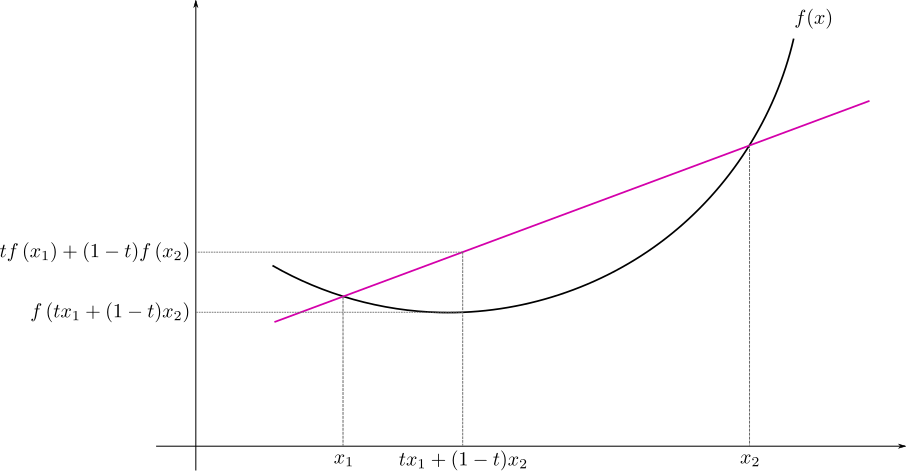
\includegraphics[width=\textwidth]{ConvexFunction}
\textbf{For the first definition}, geometrically, convexity of a function means that the points of any arc of the graph of the function lie below the chord subtended by the arc. \textbf{For the second definition}, geometrically, it means that the slope of the chord I joining $ (x_1,f(x_1)) $ to $ (x,f(x)) $ is not larger than (and in the case of strict convexity is less than) the slope of the chord II joining $ (x,f(x)) $ to $ (x_2,f(x_2)) $.
\begin{Definition}
	If the opposite inequality holds for a function $ f:(a,b )\to \Real$, that function is said to be \textit{concave} on the interval $ (a,b $, or, more often, \textit{convex upward} in the interval, as opposed to a convex function, which is then said to be \textit{convex downward} on $ (a,b) $.
\end{Definition}
\begin{Proposition}
	A necessary and sufficient condition for a function $ f:(a,b)\to \Real $ that is differentiable on the open interval $ (a,b) $ to be convex(downward) on that interval is that its derivative $ f^\prime $ be nondecreasing on $ (a,b) $. A strictly increasing $ f^\prime $ corresponds to a strict convex function.
\end{Proposition}
\begin{Corollary}
	A necessary and sufficient condition for a function $ f:(a,b)\to \Real $ having a second derivative on the open interval $ (a,b) $ to be convex(downward) on $ (a,b) $ is that $ f^{\prime\prime}(x)\geqslant 0 $ on that interval. The condition $ f^{\prime\prime}(x)> 0 $ on $ (a,b) $ is sufficient to guarantee that $ f $ is strictly convex.
\end{Corollary}
\begin{Proposition}
	A function $ f:(a,b)\to\Real $ that is differentiable on the open interval $ (a,b) $ is convex(downward) on $ (a,b) $ iff its graph contains no points below any tangent drawn to it. In that case, a necessary and sufficient condition for strict convexity is that all points of the graph except the point of tangency lie strictly above the tangent line.
\end{Proposition}
\begin{Definition}
	Let $ f:U(x_0) \to \Real $ be a function defined and differentiable on a neighborhood $ U(x_0) $ of $ x_0 \in \Real $. If the function is convex downward (resp. upward) on the set $ \mathring{U}^-(x_0)=\{x \in U(x_0) | x< x_0  \} $ and convex upward (resp. downward) on $ \mathring{U}^+(x_0)=\{x \in U(x_0) | x> x_0  \} $, then $ (x_0,f(x_0)) $ is called a \textit{point of inflection of the graph}. \textbf{The point of inflection is where the function changes its convexity.}
\end{Definition}
\begin{Proposition}[Jensen's Inequality]
	If $ f:(a,b)\to\Real $ is a convex function, $ x_1,\cdots,x_n $ are points of $ (a,b) $, and $ \alpha_1,\cdots,\alpha_n $ are nonnegative numbers such that $ \alpha_1 + \cdots + \alpha_n=1 $, then
	\begin{equation}
			f(\alpha_1 x_1+\cdots+\alpha_n x_n) \leqslant \alpha_1 f(x_1) + \cdots+\alpha_n f(x_n) \nonumber
	\end{equation}
	For a function that is convex upward, we have
		\begin{equation}
	f(\alpha_1 x_1+\cdots+\alpha_n x_n) \geqslant \alpha_1 f(x_1) + \cdots+\alpha_n f(x_n) \nonumber
	\end{equation}
\end{Proposition}
\begin{proof}
	Can be proved by induction.
\end{proof}
\begin{Example}
	Since $ f(x) =\ln x $ is strictly convex upward on the set of positive numbers, then
	\begin{equation}
			\ln(\alpha_1 x_1+\cdots+\alpha_n x_n) \geqslant \alpha_1 \ln(x_1) + \cdots+\alpha_n \ln(x_n) \nonumber
	\end{equation}
	If $ \alpha_1=\cdots=\alpha_n=\frac{1}{n} $, we have
	\begin{equation}
		\sqrt[n]{x_1\cdots x_n} \leqslant \frac{x_1+\cdots + x_n}{n} \nonumber
	\end{equation}
	between the geometric and arithmetic means of $ n $ nonnegative numbers. Equality holds only when $ x_1 = x_2 =\cdots=x_n$. By setting $ n=2 $, $ \alpha_1=\frac{1}{p} $, $ \alpha_2 = \frac{1}{q} $, $ x_1=a $, $ x_2=b $, we obtain Young's inequality for $ p>1 $.
\end{Example}

\subsection{L'Hôpital's Rule}
\begin{Proposition}[L'Hôpital's Rule]
	Suppose the function $ f:(a,b)\to\Real $ and $ g:(a,b)\to\Real $ are differentiable on the open interval $ (a,b) $ ($ -\infty \leqslant a < b \leqslant + \infty $) with $ g^\prime(x)\neq 0 $ on $ (a,b) $ and
	\begin{equation}
		\frac{f^\prime(x)}{g^\prime(x)}\to A \quad \text{ as } x \to a+0 \quad (-\infty \leqslant A \leqslant +\infty)\nonumber
	\end{equation}
	Then
	\begin{equation}
		\frac{f(x)}{g(x)} \to A \quad \text{ as } x\to a+0 \nonumber
	\end{equation}
	in each of the following two cases:\\
	1$ ^0 \quad(f(x)\to 0)\land (g(x)\to 0)$ as $ x\to a+0 $. \\
	or \\
	2$ ^0 \quad g(x)\to \infty $ as $ x\to a+0 $. \\
	A similar assertion holds as $ x \to b-0 $.
\end{Proposition}

\subsection{Constructing the Graph of a Function}
\begin{Definition}
	The line $ c_0+c_1 x $ is called an \textit{asymptote} of the graph of the function $ y=f(x) $ as $ x \to \pm \infty $ if $ f(x)-(c_0 + c_1 x) = o(1) $ as $ x \to \pm \infty $. If $ |f(x)|\to \infty $ as $ x \to a \pm 0 $, the line $ x=a $ is called a \textit{vertical asymptote} of the graph.
\end{Definition}
In general, if $ f(x)-(c_0+c_1 x+\cdots+c_n x^n)=o(1) $ as $ x \to -\infty $, then
\begin{align}
	c_n &= \lim\limits_{x \to -\infty} \frac{f(x)}{x^n} \\
	c_{n-1}&=\lim\limits_{x \to -\infty} \frac{f(x)-c_n x^n}{x^{n-1}} \\
	&\vdots \\
	c_0 &= \lim\limits_{x \to -\infty} (f(x)-(c_1 x+\cdots+c_n x^n))
\end{align}
It uses the graph of the corresponding algebraic polynomial $ c_0+c_1 x+\cdots+c_n x^n $ to describe the asymptotic behavior of $ f(x) $.
\section{Complex Numbers and Elementary Functions}
\subsection{Complex Numbers}
\begin{Example}
	The set of complex numbers, $ \Complex $, is a field containing $ \Real $ as a subfield.
\end{Example}
\begin{proof}
	The only nonobvious point in the verification that $ \Complex $ is a field is that every non-zero complex number $ z = x+\iu y $ has an inverse $ z^{-1} $. We denote the \textit{conjugate} of $ z $ as $ \tilde{z} =x- \iu y$. Then $ z^{-1} $ should be taken as $ \frac{1}{x^2+y^2}\cdot \tilde{z} =\frac{x}{x^2+y^2}- \iu \frac{y}{x^2+y^2}$.
\end{proof}
Geometrically speaking, a complex number can be viewed as the Cartesian coordinates in $ \Real^2 $. Therefore, the \textit{absolute value} or \textit{modulus} $ |z| $ of a complex number is
\begin{equation}
	|z|=\sqrt{x^2+y^2},\text{ if }z=x+ \iu y\nonumber
\end{equation}
The set of complex numbers is called the \textit{complex plane}.
\begin{Definition}
	If $ z= x+ \iu y $ (\textit{algebraic form}), then the \textit{trigonometric (polar) forms} of a complex number is
	\begin{equation}
		z= r(\cos \varphi + \iu \sin \varphi) \nonumber
	\end{equation}
	since $ x= r \cos \varphi $ and $ y= r \sin \varphi $ for $ (x,y) $ and a polar coordinate $ (r,\varphi) $. Note that $ r $ is the modulus or absolute value of $ z $. $ \varphi $ is called the \textit{argument} of $ z $ and denoted $ \varphi \in Arg z $. By the characteristics of polar coordinates, there are infinitely many representation of a complex number. To make a representation unique, we must constrain the range of the argument. If such a choice has been made(usually $ 0 \leqslant \varphi < 2 \pi $), we say that a \textit{branch} (or the \textit{principle branch}) of the argument has been chosen, thus $ \varphi = arg z $.
\end{Definition}
We can see that
\begin{equation}
	z_1 \cdot z_2 = r_1 r_2 (\cos(\varphi_1+\varphi_2)+ \iu \sin(\varphi_1+\varphi_2))\nonumber
\end{equation}
\begin{Example}[de Moivre's Formula]
	\begin{equation}
		z^n =r^n(\cos n\varphi+\iu \sin n \varphi)\nonumber
	\end{equation}
\end{Example}
The product $ az $ where $ a=|a|(\cos \varphi + \iu \sin \varphi) \neq 0 $ can be viewed as the composition of a dilation by a factor of $ |a| $ and a rotation through the angle $ \varphi \in Arg(a) $.

\subsection{Convergence in $ \Complex $ and Series with Complex Terms}
The set $ \{z \in \Complex | |z-z_0|<\varepsilon \} $, the $ \varepsilon $-neighborhood of a number $ z_0\in \Complex $ is a disk (without the boundary circle) of radius $ \varepsilon $ centered at $ z_0 $.
\begin{Definition}
	A sequence of complex terms \textit{converges} to $ z_0 \in \Complex $ if $ \lim\limits_{n \to \infty} |z_n-z_0|=0 $.
\end{Definition}
It is clear that a sequence of complex numbers converges iff the sequence of its real and imaginary parts of the terms of the sequence both converge.
The definition for a \textit{fundamental} or \textit{Cauchy} sequence in $ \Complex $ is analogous with its definition for a sequence of real numbers.
\begin{Proposition}[The Cauchy Criterion]
	A sequence of complex numbers converges iff it is a Cauchy sequence.
\end{Proposition}
The Cauchy Criterion for series and the definition of absolute convergence is the same as them for a series of real numbers.
\begin{Proposition}[The Cauchy-Hadmard Formula]
	The power series
	\begin{equation}
		c_0+c_1(z-z_0)+\cdots+c_n(z-z_0)^n+\cdots \nonumber
	\end{equation}
	converges inside the disk $ |z-z_0|< R $ with center at $ z_0 $ and radius given by the Cauchy-Hadamard formula
	\begin{equation}
		R =\frac{1}{\varlimsup_{n \to \infty} \sqrt[n]{|c_n|}} \nonumber
	\end{equation}
	At any point exterior to this disk the power series diverges. \\
	At any point interior to the disk, the power series converges absolutely.
\end{Proposition}
\begin{Proposition}[Abel's First Theorem on Power Series]
	If the power series converges at some value $ z^* $, then it absolutely converges for any value of $ z $ satisfying the inequality $ |z-z_0|<|z^*-z_0| $.
\end{Proposition}
\begin{Proposition}
	If a series of complex numbers converges absolutely, then a series obtained by rearranging its terms also converges absolutely and has the same sum.
\end{Proposition}
\begin{Proposition}
	The product of absolute convergent series is an absolutely convergent series whose sum equals the product of the sums of the factor series.
\end{Proposition}
\begin{Example}
	For two series $ \sum_{n=0}^{\infty}\frac{1}{n!}a^n $ and $ \sum_{m=0}^{\infty}\frac{1}{m!}b^m $ that converge absolutely, if $ k=m+n $, we have
	\begin{equation}
		\sum_{n=0}^{\infty}\frac{1}{n!}a^n \cdot \sum_{m=0}^{\infty}\frac{1}{m!}b^m = \sum_{k=0}^{\infty}\frac{1}{k!}(a+b)^k\nonumber
	\end{equation}
\end{Example}

\subsection{Euler's Formula and the Connections Among the Elementary Functions}
\begin{Theorem}[Euler Formula]
	\begin{equation}
		e^{\iu y}=\cos y+ \iu \sin y \nonumber
	\end{equation}
	Here $ y $ is either a real number or an arbitrary number. If $ y=0 $
	\begin{equation}
		e^{\iu \pi} +1= 0\nonumber
	\end{equation}
\end{Theorem}
\begin{proof}
	Find the Taylor series for $ e^z,\cos z, \sin z $, where $ z \in \Complex$ , then substitute $ z $ with $ \iu y $.
\end{proof}
\begin{Definition}[The Trigonometric Notation for a Complex Number]
	\begin{equation}
		z = r e^{\iu \varphi} \nonumber
	\end{equation}
	where $ r $ is the modulus of $ z $ and $ \varphi $ its argument.
\end{Definition}
\begin{Theorem}[Formula of de Moivre]
	\begin{equation}
		z^n=r^n e^{\iu n \varphi} \nonumber
	\end{equation}
\end{Theorem}



\subsection{Power Series Representation of a Function. Analyticity}
\begin{Theorem}
	\begin{equation}
		a^n-b^n = (a-b)(a^{n-1} + a^{n-2}b + \cdots + b^{n-1}) \nonumber
	\end{equation}
\end{Theorem}
\begin{proof}
	\begin{align}
	(a-b)\sum_{i=0}^{n-1}a^ib^{n-1-i}&=\sum_{i=0}^{n-1}a^{i+1}b^{n-1-i}-\sum_{i=0}^{n-1}a^ib^{n-i}\\
	&=\sum_{i=0}^{n-1}(a^{i+1}b^{n-(i+1)}-a^ib^{n-i})\\
	&=a^n-b^n
	\end{align}
	an alternative proof uses the fact that for $ x \neq 1 $
	\begin{equation}
		1+x+ \cdots + x^{n-1} = {1-x^n \over 1-x} \nonumber
	\end{equation}
	If $ a=b $ or $ a=0 $, then the theorem is obviously true. When $ a \neq 0 $ and $ a \neq b $, set $ x=\frac{b}{a} $ in the sum of the geometric series above and multiply the result by $ a^n $.
\end{proof}
A complex function has complex domain and complex range, thus its graph is a subset of $ \Complex \times \Complex = \Real^4 $ and can not be visualized in the traditional way. To compensate for this loss to some extent, one usually keeps two copies of the complex plane $ \Complex $, indicating points of the domain in one and points of the range of values in the other.\newpara
The definitions of continuity, derivative, and differentiability for complex-valued functions are identical to those for real-valued functions. Since the arithmetic properties of the fields $ \Complex $ and $ \Real $ are the same, all the general rules for differentiation, such as rules for addition, product, and quotient also hold.
\begin{Theorem}
	The sum $ f(z)= \sum_{n=0}^{\infty} c_n (z-z_0)^n $ of a power series is an infinitely differentiable function inside the entire disk in which convergence occurs. Moreover,
	\begin{align}
	\Aboxed{f^{(k)}(z)= \sum_{n=0}^{\infty}\frac{d^k}{d z^k}(c_n (z-z_0)^n), \quad k=0,1,\cdots}\nonumber
	\end{align}
	and 
	\begin{equation}
		c_n=\frac{1}{n!}f^{(n)}(z_0),\quad n=0,1,\cdots \nonumber
	\end{equation}
\end{Theorem}
\begin{proof}
	The expressions for the coefficient follows from the expressions for $ f^{(k)}(z) $ for $ k=n $ and $ z=z_0 $. As for the formula for $ f^{(k)}(z) $, it suffices to verify this formula for $ k=1 $, since the function $ f^\prime(z) $ will then be the sum of a power series. Thus, we'll verify that the function $ \varphi(z)=\sum_{n=1}^{\infty}n c_n(z-z_0)^{n-1} $ is the derivative of $ f(z) $. \newpara
	By the Cauchy-Hadamard formula, the radius of convergence of the derived series is the same as the radius of convergence $ R $ of the original power series. For simplicity of notion we shall assume that $ z_0=0 $ and the series converge for $ |z|<R $. \newpara
	Since a power series converges absolutely on the interior of its disk of convergence, the estimate $ |nc_n z^{n-1}|=n|c_n||z|^{n-1}\leqslant n|c_n|r^{n-1} $ holds for $ |z| \leqslant r <R $, and that series $ \sum_{n=1}^{\infty}n|c_n|r^{n-1}  $ converges. Hence, for any $ \varepsilon>0 $ there exists an index $ N $ such that
	\begin{equation}
		|\sum_{n=N+1}^{\infty}nc_n z^{n-1}|\leqslant |\sum_{n=N+1}^{\infty}nc_n r^{n-1}|\leqslant \frac{\varepsilon}{3} \nonumber
	\end{equation}
	for $ |z|\leqslant r $. Thus at any point of the disk $ |z|<r $ the function $ \varphi(z) $ is within $ \frac{\varepsilon}{3} $ of the $ N $th partial sum of the series that defines it.
	\newpara
	Now let $ \zeta $ and $ z $ be arbitrary points of this disk. The transformation
	\begin{align}
		\frac{f(\zeta)-f(z)}{\zeta - z} &= \sum_{n=1}^{\infty}c_n \frac{\zeta^n-z^n}{\zeta -z}=\\
		&=\sum_{n=1}^{\infty}c_n(\zeta^{n-1}+\zeta^{n-1}z+\cdots+\zeta z^{n-2}+z^{n-1}) \nonumber
	\end{align}
	and the estimation $ |c_n(\zeta^{n-1}+\cdots+z^{n-1})\leqslant |c_n|n r^{n-1} $ enable us to conclude that the difference quotient is equal within $ \frac{\varepsilon}{3} $ to the partial sum of the series that defines it, provided $ |\zeta|<r $ and $ |z|<r $. Hence, for $ |\zeta|<r $ and $ |z|<r $ we have
	\begin{equation}
		|\frac{f(\zeta)-f(z)}{\zeta - z} - \varphi(z)|\leqslant |\sum_{n=1}^{N}c_n \frac{\zeta^n-z^n}{\zeta -z}-\sum_{n=1}^{N}n c_n z^{n-1}|+2\frac{\varepsilon}{3} \nonumber
	\end{equation}
	If we now fix $ z $ and let $ \zeta $ tend to $ z $, passing to the limit in the finite sum, we see that the right-hand side of this last inequality will be less than $ \varepsilon $ for $ \zeta $ sufficiently close to $ z $, and hence the left-hand side will be also.
	\newpara
	Thus, for any point $ z $ in the disk $ |z|<r<R $, we have verified that $ f^\prime(z)=\varphi(z) $. Since $ r $ is arbitrary, this relation holds for any point of the disk $ |z|<R $.
\end{proof}
\begin{Definition}
	A function is \textit{analytic} at a point $ z_0 \in \Complex $ if it can be represented in a neighborhood of the point in the following ("analytic") form:
	\begin{equation}
		f(z)=\sum_{n=0}^{\infty}c_n (z-z_0)^n \nonumber
	\end{equation}
	that is, as the sum of a power series in $ z-z_0 $.
\end{Definition}
\begin{Corollary}
	\textbf{a)} If a function is analytic at a point, then it is infinitely differentiable at that point, and its Taylor series converges to it in a neighborhood of the point. \newpara
	\textbf{b)} The Taylor series of a function defined in a neighborhood of a point and infinitely differentiable at that point converges to the function in some neighborhood of the point iff the function is analytic.
\end{Corollary}
This means that if a function has one derivative in a neighborhood of a point, it also has derivatives of all orders in that neighborhood.

\subsection{Algebraic Closedness of the Field $ \Complex $ of Complex Numbers}
\begin{Theorem}[Fundamental Theorem of Algebra]
	Every polynomial
	\begin{equation}
		P(z)=c_0 + c_1 z + \cdots + c_n z^n \nonumber
	\end{equation}
	of degree $ n \geqslant 1 $ with complex coefficients has a root in $ \Complex $.
\end{Theorem}
\begin{proof}
	Without loss of generality, we may obviously assume that $ c_n=1 $(replace $ 1 $ with $ c_n $ won't cause significant change to the rest of the proof).\newpara
	Let $ \mu=\inf_{z \in \Complex}|P(z)|$. Since $ P(z)=z^n(1+\frac{c_n-1}{z}+\cdots + \frac{c_0}{z^n}) $, we have
	\begin{equation}
		|P(z)|\geqslant |z|^n (1-\frac{|c_{n-1}|}{|z|}-\cdots-\frac{|c_0|}{|z|^n}) \nonumber
	\end{equation}
	and obviously $ |P(z)|>\max \{1,2\mu \} $ for $ |z|>R $ if $ R $ is sufficiently large. Consequently, the points of a sequence $ \{z_k \} $ at which $ 0<|P(z_k)|-\mu < \frac{1}{k} $(the sequence converges to $ \mu $) lie inside the disk $ |z|<R $.\newpara
	Next step is to verify that there is a point $ z_0\in\Complex $(in fact, in this disk) at which $ |P(z_0)|=\mu $. We remark that if $ z_k=x_k+\iu y_k $, then $ \max\{|x_k|,|y_k| \}\leqslant |z_k| \leqslant R $ and hence the sequence of real numbers $ \{x_k\} $ and $ \{y_k\} $ are bounded. By the Bolzano-Weierstrass lemma, choosing first a convergent subsequence $ \{x_{k_{l_m}} \} $ from $ \{x_k\} $ and then a convergent subsequence $ \{y_{k_{l_m}} \} $ from $ \{y_{k} \} $, we obtain a subsequence $ z_{k_{lm}} =x_{k_{l_m}}+\iu y_{k_{l_m}}$ of the sequence $ \{z_k \} $ that has a limit $ \lim\limits_{m \to \infty}z_{k_{l_m}}= \lim\limits_{m\to \infty}x_{k_{l_m}}+\iu \lim\limits_{m \to \infty}y_{k_{l_m}}=x_0 + \iu y_0 = z_0$, and since $ |z_{k_{l_m}} \to |z_0|$ as $ m \to \infty $, it follows that $ |z_0|\leqslant R $. So as to avoid cumbersome notation, and not have to pass to subsequences, we shall assume that the sequence $ \{z_k\} $ itself converges. It follows from the continuity of $ P(z) $ at $ z_0 \in \Complex $ that $ \lim\limits_{k \to \infty}P(z_k)=P(z_0) $. But then $ |P(z_0)|=\lim\limits_{k \to \infty}|P(z_k)|=\mu $. \newpara
	We shall now assume that $ \mu >0 $, and use this assumption to derive a contradiction. If $ P(z_0)\neq 0 $, consider the polynomial $ Q(z)=\frac{P(z+z_0)}{P(z_0)} $. By construction $ Q(0)=1 $ and $ |Q(z)|=|\frac{P(z+z_0)}{P(z_0)}| \geqslant 1$. \newpara
	Since $ Q(0) =1$, the polynomial $ Q(z) $ has the form
	\begin{equation}
		Q(z)=1+q_k z^k + q_{k+1}z^{k+1}+\cdots + q_n z^n \nonumber
	\end{equation}
	where $ |q_k|\neq 0 $ and $ 1 \leqslant k \leqslant n $. If $ q_k=\rho e^{\iu \psi} $, then for $ \varphi = \frac{\pi-\psi}{k} $ we shall have $ q_k \cdot (e^{\iu \varphi})^k = \rho e^{\iu \psi}e^{\iu (\pi-\psi)}=\rho e^{\iu \pi}=-\rho = -|q_k| $. Then, for $ z=re^{\iu \varphi} $ we obtain
	\begin{align}
		|Q(re^{\iu \varphi})&\leqslant |1+q_k z^k| + (|q_{k+1}z^{k+1}|+\cdots + |q_n z^n| )=\\
		&=|1-r^k|q_k||+r^{k+1}(|q_{k+1}|+\cdots+|q_n|r^{n-k-1})=\\
		&=1-r^k(|q_k|-r|q_{k+1}|-\cdots-r^{n-k}|q_n|)<1 
	\end{align}
	if $ r $ is sufficiently close to $ 0 $. But $ |Q(z)|\geqslant 1 $ for $ z \in \Complex $. This contradiction shows that $ P(z_0)=0 $.
\end{proof}
\textit{Remark} If $ P(z_0)=0 $, then its conjugate $ \tilde{z_0} $ satisfies $ P(\tilde{z_0})=0 $.
\begin{Corollary}
	Every polynomial $ P(z)=c_0 + \cdots + c_n z^n $ of degree $ n \geqslant 1 $ with complex coefficients admits a representation in the form
	\begin{equation}
		P(z)=c_n(z-z_1)\cdots(z-z_n) \nonumber
	\end{equation}
	where $ z_1, \cdots, z_n \in \Complex $(they are not necessarily all distinct). This representation is unique up to the order of the factors.
\end{Corollary}
\begin{proof}
	Use the long division algorithm on $ P(z) $, we find that $ P(z)=q(z)Q(z)+r(z) $, where $ q(z) $ and $ r(z) $ are polynomials, the degree of $ r(z) $ being less than the degree $ m $ of $ Q(z) $. Thus if $ m=1 $, then $ r(z) $ is simply a constant. \newpara
	Let $ z_1 $ be a root of the polynomial $ P(z) $. Then $ P(z)=q(z)(z-z_1)+r $, and since $ P(z_1)=r $, it follows that $ r=0 $. Hence if $ z_1 $ is a root of $ P(z) $, we have the representation $ P(z)=(z-z_1)q(z) $. The degree of the polynomial $ q(z) $ is $ n-1 $, and we can repeat the reasoning with $ q(z) $ if $ n-1 \geqslant 1 $. By induction we find that $ P(z)=c(z-z_1)\cdots(z-z_0) $. Since we must have $ c z_n=c_n z^n $, it follows that $ c=c_n $.
\end{proof}
By multiplying out all identical factors, one can rewrite that product:
\begin{equation}
	P(z)=c_n(z-z_1)^{k_1}\cdots(z-z_n)^{k_p} \nonumber
\end{equation}
The number $ k_j $ is called the \textit{multiplicity} of the root $ z_j $.
\begin{Corollary}
	Every polynomial $ P(z)=a_0+\cdots+a_n z^n $ with real coefficients can be expanded as a product of linear and quadratic polynomials with real coefficients.
\end{Corollary}
\begin{Corollary}
	Every root $ z_j $ of multiplicity $ k_j>1 $ of a polynomial $ P(z) $ is a root of multiplicity $ k_j -1 $ of the derivative $ P^\prime(z) $.
\end{Corollary}
\begin{Corollary}
	\textbf{a)} If $ Q(z)=(z-z_1)^{k_1} \cdots (z-z_p)^{k_p} $ and $ \frac{P(z)}{Q(z)} $ is a proper fraction (the degree of $ P(z) $ is less than that of $ Q(z) $), there exists a unique representation of the fraction $ \frac{P(z)}{Q(z)} $ in the form
	\begin{equation}
		\frac{P(z)}{Q(z)}=\sum_{j=1}^{p}(\sum_{k=1}^{k_j}\frac{a_{jk}}{(z-z_j)^k}) \nonumber
	\end{equation}
	\textbf{b)} If $ P(x) $ and $ Q(x) $ are polynomials with real coefficients and
	\begin{equation}
		Q(x)=(x-x_1)^{k_1} \cdots (x-x_l)^{k_l}(x^2+p_1 x + q_1)^{m_1} \cdots (x^2 + p_n x + q_n)^{m_n} \nonumber
	\end{equation}
	there exists a unique representation of the proper fraction $ \frac{P(x)}{Q(x)} $ in the form
	\begin{equation}
		\frac{P(x)}{Q(x)} = \sum_{j=1}^{l}(\sum_{k=1}^{k_j}\frac{a_{jk}}{(x-x_j)^k}) + \sum_{j=1}^{j=1}(\sum_{k=1}^{m_j}\frac{b_{jk}x+c_{jk}}{(x^2+p_j x + q_j)^k}) \nonumber
	\end{equation}
	where $ a_{jk},b_{jk} $, and $ c_{jk} $ are real numbers.
\end{Corollary}


\section{Primitives}
\subsection{The Primitive and the Indefinite Integral}
\begin{Definition}
	A function $ F(x) $ is a \textit{primitive} of a function $ f(x) $ on an interval if $ F $ is differentiable on the interval and satisfies the equation $ F^\prime(x)=f(x) $, or $ d F(x)=f(x)dx $.
\end{Definition}

\begin{Proposition}
	From Lagrange's theorem, if $ F_1(x) $ and $ F_2(x) $ are two primitives of $ f(x) $ on the same interval, then the difference $ F_1(x)-F_2(x) $ is constant on that interval.
\end{Proposition}
\begin{Definition}
	The \textit{indefinite integral} of $ f(x) $ is denoted as
	\begin{equation}
		\int f(x)dx \nonumber
	\end{equation}
	where $ \int $ is called the \textit{indefinite integral sign}, $ f $ is called the \textbf{integrand}, and $ f(x)dx $ is called a \textit{differential form}.
\end{Definition}

\subsection{The Basic General Methods of Finding a Primitive}
\begin{Theorem}
	Taken account of the relationship between a function and its primitive as well as the laws of differentiation, we can assert that the following relations hold
	\begin{align}
		&\text{a. }\quad \int(\alpha u(x)+\beta v(x))dx = \alpha \int u(x)dx+\beta \int v(x)dx +c \\
		&\text{b. }\quad \int(uv)^\prime dx = \int u^\prime(x)v(x)dx + \int u(x)v^\prime(x)dx +c
	\end{align}
	Moreover, if
	\begin{equation}
		\int f(x)dx = F(x)+c \nonumber
	\end{equation}
	on an interval $ I_x $ and $ \varphi:I_t  \to I_x$ is a smooth (continuously differentiable) mapping of the interval $ I_t $ into $ I_x $, then
	\begin{equation}
		\int (f \circ \varphi)(t)\varphi^\prime(t)dt = (F \circ \varphi)(t)+c \nonumber
	\end{equation}
	Here we make the change of variable $ \varphi(t)=x $. This can be used to find primitive.
\end{Theorem}
\begin{Example}[Integration by Parts]
	\begin{equation}
		\int(uv)^\prime dx = \int u^\prime(x)v(x)dx + \int u(x)v^\prime(x)dx+c \nonumber
	\end{equation}
	can be rewritten as
	\begin{equation}
		\int u(x)dv(x) = u(x)v(x)-\int v(x)du(x)+c \nonumber
	\end{equation}
\end{Example}
Some primitives of the composition of elementary functions \textbf{cannot be expressed as the composition of elementary functions}. We make the following definition for special cases of indefinite integrals:
\begin{Definition}[Sine Integral]
	The \textit{sine integral}, denoted $ \Si x $, is defined as
	\begin{equation}
		\Si x = \int \frac{\sin x}{x}dx \nonumber
	\end{equation}
\end{Definition}
\begin{Definition}[Cosine Integral]
	The \textit{cosine integral}, denoted $ \Ci x $, is defined as
	\begin{equation}
	\Ci x = \int \frac{\cos x}{x}dx \nonumber
	\end{equation}
\end{Definition}
\begin{Definition}[Logarithmic Integral]
	The \textit{logarithmic integral}, denoted $ \li x $, is defined as
	\begin{equation}
	\li x = \int \frac{ dx}{\ln x} \nonumber
	\end{equation}
\end{Definition}

\subsection{Primitives of Rational Functions}
\begin{Example}
	\begin{equation}
		\int \frac{1}{(x-a)^k}dx = \begin{cases}
		& \frac{1}{-k+1}(x-a)^{-k+a}+c\quad \text{for }k \neq 1\\
		&\ln |x-a|+c \quad \text{for }k=1\\
		\end{cases} \nonumber
	\end{equation}
\end{Example}
\begin{Example}
	For the following integral
	\begin{equation}
		\int \frac{bx+c}{(x^2+px+q)^k}dx \nonumber
	\end{equation}
	We represent $ x^2+px+q $ as $ (x+\frac{1}{2}p)^2 +(p-\frac{1}{4}p^2)$, where $ q- \frac{1}{4}p^2>0 $, since the original polynomial has no real roots. Setting $ x+ \frac{1}{2}p=u $ and $ q-\frac{1}{4}p^2 =a^2 $, we obtain
	\begin{equation}
		\int \frac{bx+c}{(x^2+px+q)^k}dx = \int \frac{\alpha u + \beta}{(u^2+a^2)^k}du \nonumber
	\end{equation}
	where $ \alpha = b $ and $ \beta = c- \frac{1}{2}bp $. Next
	\begin{equation}
		\int \frac{\alpha u + \beta}{(u^2+a^2)^k}du = \begin{cases}
		& \frac{1}{2(1-k)}(u^2+a^2)^{-k+1}\quad \text{for }k\neq 1\\
		& \frac{1}{2}\ln(u^2+a^2)\quad \text{for }k=1\\
		\end{cases} \nonumber
	\end{equation}
\end{Example}
\begin{Example}
	For the following integral
	\begin{equation}
		I_k = \int \frac{du}{(u^2+a^2)^k} \nonumber
	\end{equation}
	Integrating by parts and making elementary transformations, we have
	\begin{equation}
		I_k = \frac{u}{(u^2+a^2)^k} + 2k I_k - 2k a^2 I_{k+1} \nonumber
	\end{equation}
	which makes it possible to lower the exponent $ k $ in the integral. But $ I_1 $ is easy to compute
	\begin{equation}
		I_1 = \frac{1}{a}\arctan \frac{u}{a} +c \nonumber
	\end{equation}
	and then we can compute the primitive our original problem.
\end{Example}
\begin{Proposition}
	The primitive of any rational function $ R(x)=\frac{P(x)}{Q(x)} $ can be expressed in terms of rational functions and the transcendental functions $ \ln $ and $ \arctan $. The rational part of the primitive, when placed over a common denominator, will have a denominator containing all the factors of the polynomial $ Q(x) $ with multiplicities one less than they have in $ Q(x) $.
\end{Proposition}
\begin{Example}
	For the indefinite integral
	\begin{equation}
		\int\frac{2x^2+5x+5}{(x^2-1)(x+2)}dx \nonumber
	\end{equation}
	We find all the factors of the denominator, then
	\begin{equation}
		\frac{2x^2+5x+5}{(x^2-1)(x+2)} = \frac{A}{x-1}+\frac{B}{x+1}+\frac{C}{x+2} \nonumber
	\end{equation}
	Putting the right-hand side of this equation over a common denominator
	\begin{equation}
		\frac{2x^2+5x+5}{(x^2-1)(x+2)} = \frac{(A+B+C)x^2+(3A+B)x+(2A-2B-C)}{(x-1)(x+1)(x+1)} \nonumber
	\end{equation}
	 and solve the system
	 \begin{equation}
	 	\begin{cases}
	 	&A+B+C=1\\
	 	&3A+B=5\\
	 	&2A-2B-C=5\\
	 	\end{cases} \nonumber
	 \end{equation}
\end{Example}




\subsection{Primitives of the Form $ \int R(\cos x, \sin x)dx $}
Let $ R(u,v) $ be a rational function in $ u $ and $ v $, that is a quotient of polynomials $ \frac{P(u,v)}{Q(u,v)} $, which are linear combinations of monomials $ u^m v^n $, where $ m=0,1,2,\cdots $ and $ n=0,1,\cdots $. \newpara
\textbf{a.} We make the change of variable $ t=\tan \frac{x}{2} $, and
\begin{equation}
	\int R(\cos, \sin x)dx = \int R(\frac{1-t^2}{1+t^2},\frac{2t}{1+t^2})\frac{2}{1+t^2}dt \nonumber
\end{equation}
\textbf{b.} In the case of $ \int R(\cos^2 x, \sin^2 x)dx $ or $ \int r(\tan x)dx $, where $ r(u) $ is a rational function, we substitute $ t $ with $ \tan x $, and
\begin{align}
	\int R(\cos^2 x, \sin^2 x)dx &= \int R(\frac{1}{1+t^2},\frac{t^2}{1+t^2})\frac{dt}{1+t^2} \nonumber\\
	\int r(\tan x)dx  &= \int r(t)\frac{dt}{1+t^2}\nonumber
\end{align}
\textbf{c.} In the case of integrals of the form
\begin{equation}
	\int R(\cos x, \sin^2 x)\sin x dx \quad \text{ or }\quad \int R(\cos^2 x, \sin x)\cos x dx \nonumber
\end{equation}
One can move the functions $ \sin x $ and $ \cos x $ into the differential and make the substitution $ t=\cos x $ or $ t = \sin x $ respectively. Then
\begin{equation}
	- \int R(t,1-t^2)dt \quad \text{or } \quad \int R(1-t^2,t)dt \nonumber
\end{equation}


\subsection{Primitives of the Form $ \int R(x,y(x))dx $}
Let $ R(x,y) $, as in previous subsection, a rational function where $ y $ is a function of $ x $. \newpara
\textbf{a.} If $ y =\sqrt[n]{\frac{ax+b}{cx+d}}$, where $ n \i \Natural $, then, setting $ t^n = \frac{ax+b}{cx+d} $, we obtain
\begin{equation}
	x=\frac{d \cdot t^n-b}{a-c\cdot t^n},\quad y=t \nonumber
\end{equation}
\textbf{b.} When $ y=\sqrt{ax^2+bx+c} $, we reduce the general case to one of the following three simple cases by completing the square in the trinomial $ ax^2+bx+c $ and making a suitable linear substitution
\begin{equation}
	\int R(t,\sqrt{t^2+1})dt,\quad \int R(t,\sqrt{t^2-1})dt,\quad \int R(t,\sqrt{1-t^2})dt \nonumber
\end{equation}
Now we make the following substitutions
\begin{align}
	&\sqrt{t^2+1}=tu+1,\quad \text{or } \quad \sqrt{t^2+1}=tu-1,\quad \text{or }\quad \sqrt{t^2+1}=t-u\\
	&\sqrt{t^2-1}=u(t-1),\quad \text{or } \quad \sqrt{t^2-1}=u(t+1),\quad \text{or }\quad \sqrt{t^2-1}=t-u\\
	&\sqrt{1-t^2}=u(1-t),\quad \text{or } \quad \sqrt{1-t^2}=u(1+t),\quad \text{or }\quad \sqrt{1-t^2}=tu \pm 1\\
\end{align}
that will reduce these integrals to the integral of a rational function. Alternatively, one can make the substitution $ t= \sinh \varphi ,t=\cosh \varphi$, and $ t= \sin \varphi $ (or $ t= \cos \varphi $) respectively.\newpara
\textbf{c.Elliptic Integrals} 
\begin{Definition}[Elliptic Integrals]
	\begin{equation}
		\int R(x,\sqrt{P(x)})dx \nonumber
	\end{equation}
	Here $ P(x) $ is a polynomial of degree $ n>2 $. In general, such an integral cannot be expressed in terms of elementary functions. For $ n=3 $ and $ n=4 $, this integral is called an \textit{elliptic integral}, and for $ n>4 $ it is called \textit{hyperelliptic}.
\end{Definition}
By elementary substitutions the general elliptic integral can be reduced to the following three standard forms up to terms expressible in elementary functions:
\begin{align}
	&\int \frac{dx}{\sqrt{(1-x^2)(1-k^2x^2)}}, \\
	&\int \frac{x^2 dx}{\sqrt{(1-x^2)(1-k^2x^2)}}, \\
	&\int \frac{dx}{(1+hx^2)\sqrt{(1-x^2)(1-k^2x^2)}}
\end{align}
where $ h $ and $ k $ are parameters and $ k \in (0,1)$. By the substitution $ x = \sin \varphi $, we reduce all these three integrals to:
\begin{align}
	&\int \frac{d \varphi}{\sqrt{1-k^2 \sin^2 \varphi}}, \\
	&\int \sqrt{1-k^2 \sin^2 \varphi}d\varphi, \\
	&\int \frac{d \varphi}{(1+h \sin^2 \varphi)\sqrt{1-k^2 \sin^2 \varphi}}
\end{align}
The integrals are called respectively the \textit{elliptic integral of \textbf{first kind}, \textbf{second kind},} and \textit{\textbf{third kind}} (in the Legendre form).\newpara
The symbols $ F(k,\varphi) $ and $ E(k,\varphi) $ respectively denote the particular elliptic integrals of first and second kind that satisfy $ F(k,0)=0 $ and $ E(k,0)=0 $.



\chapter{Integration}
\section{Definition of the Integral and Description of the Set of Integrable Functions}
\subsection{Definition of the Riemann Integral}
\subsubsection{Partitions}
\begin{Definition}
	A \textit{partition} $ P $ of a closed interval $ [a,b] $, is a finite system of points $ x_0,\cdots,x_n $ of the interval such that $ a=x_0<x_1<\cdots<x_n=b $. \\
	The intervals $ [x_{i-1},x_i],(i=1,\cdots,n) $ are called the \textit{intervals} of the partition $ P $.\\
	The largest of the lengths of the intervals of the partition $ P $, denoted $ \lambda(P) $, is called the \textit{mesh} of the partition.\newpara
	\textbf{An alternative definition for a partition}: Let A be a nonempty class and $ \{A_i | i\in I \} $ a family of subsets of $ A $ such that
	\begin{align}
		&\forall i \in I (A_i \neq \varnothing)\\
		&\bigcup_{i \in I}A_i = A;\\
		&\forall i\neq j \in I(A_i \cap A_j = \varnothing)
	\end{align}
	then $ \{A_i | i\in I \} $ is said to be a \textit{partition} of $ A $.
\end{Definition}
\begin{Definition}
	We speak of a \textit{partition with distinguished points} $ (P,\xi) $ on $ [a,b] $ if we have a partition $ P $ of $ [a,b] $ and a point $ \xi_i \in [x_{i-1},x_i] $ has been chosen in each of the intervals. The set of points $ (\xi_1,\cdots,\xi_n) $ is denoted by the single letter $ \xi $.
\end{Definition}
\subsubsection{A Base in the Set of Partitions}
The base $ \mathcal{B}=\{B_d\} $ where $ d>0 $ consists of all partitions with distinguished points $ (P,\xi) $ on $ [a,b] $ for which $ \lambda(P)<d $.
\subsubsection{Riemann Sums}
\begin{Definition}
	If a function $ f $ is defined on $ [a,b] $ and $ (P,\xi) $ is a partition with distinguished points on this closed interval, the sum
	\begin{equation}
		\sigma (f,P,\xi)\coloneqq \sum_{i=1}^{n}f(\xi_i)\Delta x_i \nonumber
	\end{equation}
	where $ \Delta x_i = x_i - x_{i-1} $, is the \textit{Riemann sum} of the function $ f $ corresponding to the partition $ (P,\xi) $ on $ [a,b] $.
\end{Definition}
When the function $ f $ is fixed, the Riemann sum is a function $ \Phi(p)=\sigma (f,p) $ on the set $ \mathcal{P} $ of all partitions $ p=(P,\xi) $ on $ [a,b] $.
\subsubsection{The Riemann Integral}
\begin{Definition}
	The number $ I $ is the Riemann integral of the function $ f $ on the closed interval $ [a,b] $ if for every $ \varepsilon>0 $ there exists $ \delta>0 $ such that
	\begin{equation}
		|I-\sum_{i=1}^{n}f(\xi_i)\Delta x_i|<\varepsilon \nonumber
	\end{equation}
	for any partition $ (P,\xi) $ on $ [a,b] $ whose mesh $ \lambda(P) $ is less than $ \delta $. The definition is equivalent to the statement
	\begin{equation}
		I = \lim\limits_{\mathcal{B}}\Phi(p)\nonumber
	\end{equation}
	The integral of $ f(x) $ over $ [a,b] $ is denoted
	\begin{equation}
		\int_{a}^{b}f(x)dx \nonumber
	\end{equation}
	in which the numbers $ a $ and $ b $ are called respectively the \textit{lower} and \textit{upper limits of integration}. The function $ f $ is called the \textit{integrand}, $ f(x)dx $ is called the \textit{differential form}, and $ x $ is the \textit{variable of integration}. Thus
	\begin{align}
		\Aboxed{\int_{a}^{b}f(x)dx \coloneqq \lim\limits_{\lambda(p)\to 0}\sum_{i=1}^{n}f(\xi_i)\Delta x_i   }
	\end{align}
\end{Definition}
\begin{Definition}
	A function $ f $ is \textit{Riemann integrable} on $ [a,b] $ if the Riemann integral of $ f $ is defined on $ [a,b] $. The set of Riemann-integrable functions on a closed interval $ [a,b] $ will be denoted $ \mathcal{R}[a,b] $.
\end{Definition}

\subsection{The Set of Integrable Functions}
\subsubsection{A Necessary Condition for Integrability}
\begin{Proposition}
	A necessary condition for a function $ f $ defined on a closed interval to be Riemann integrable on it is that $ f $ be bounded on this closed interval.
\end{Proposition}
\subsubsection{A Sufficient Condition for Integrability and the Most Important Classes of Integrable Functions}
\begin{Theorem}[Reverse Triangle Inequality]
	In a normed vector space
	\begin{equation}
		|\norm{x}-\norm{y}| \leqslant \norm{x-y} \nonumber
	\end{equation}
	Or for metric spaces
	\begin{equation}
		|d(y,x)-d(x,z)|\leqslant d(y,z) \nonumber
	\end{equation}
\end{Theorem}
\begin{proof}
	Use the regular triangle inequality.
\end{proof}
\begin{Definition}
	If a partition $ \tilde{P} $ of $ [a,b] $ is obtained from the partition $ P $ by adjunction of new points to $ P $, $ \tilde{P} $ is called a \textit{refinement} of $ P $.
\end{Definition}
\begin{Proposition}
	A sufficient condition for a bounded function $ f $ to be integrable on a closed interval $ [a,b] $ is that for every $ \varepsilon>0 $ there exists a number $ \delta>0 $ such that
	\begin{equation}
		\sum_{i=1}^{n}\omega(f,\Delta_i)\Delta x_i <\varepsilon \nonumber
	\end{equation}
	for any partition $ P $ of $ [a,b] $ with mesh $ \lambda(P)<\delta $.
\end{Proposition}
\begin{proof}
	Under the sufficient condition given in the statement, for any $ \varepsilon>0 $ we can find $ \delta >0 $ such that
	\begin{equation}
		|\sigma(f,\tilde{P},\tilde{\xi})-\sigma(f,P,\xi)|<\frac{\varepsilon}{2} \nonumber
	\end{equation}
	for any partition $ P $ of $ [a,b] $ with $ \lambda(P)<\delta $. Now if $ (P^\prime,\xi^\prime) $ and $ (P^{\prime\prime},\xi^{\prime\prime}) $ are arbitrary partitions with distinguished points on $ [a,b] $ whose mashed satisfy $ \lambda(P^\prime)<\delta $ and $ \lambda(P^{\prime\prime})<\delta $, then the partition $ \tilde{P}= P^\prime \cup P^{\prime\prime}$ must satisfy the inequality above. Add these two inequality with the proper substitution while taking account of the triangle inequality and reverse triangle inequality, we have
	\begin{equation}
		|\sigma(f,P^\prime,\xi^\prime)-\sigma(f,P^{\prime\prime},\xi^{\prime\prime})|<\varepsilon \nonumber
	\end{equation}
	then by the Cauchy criterion, the limit of the Riemann sums exists.
\end{proof}

\begin{Corollary}
	$ (f\in C[a,b])\Rightarrow (f\in \mathcal{R}[a,b]) $, that is, every continuous function on a closed interval is integrable on that closed interval.
\end{Corollary}
\begin{proof}
	If a function is continuous on a closed interval, it is bounded on that interval. A continuous function on a closed interval is also uniformly continuous on the interval. Therefore, for every $ \varepsilon>0 $ there exists $ \delta>0 $ such that $ \omega(f,\Delta)<\frac{\varepsilon}{b-a} $ on any closed interval $ \Delta \subset [a,b] $ of length less than $ \delta $. Then for any partition $ P $ with $ \lambda(P)<\delta $ we have
	\begin{equation}
		\sum_{i=1}^{n}\omega(f,\Delta_i)\Delta_{x_i}<\frac{\varepsilon}{b-a}\sum_{i=1}^{n}\Delta_{x_i}=\frac{\varepsilon}{b-a}(b-a)=\varepsilon \nonumber
	\end{equation}
\end{proof}
\begin{Corollary}
	If a bounded function $ f $ on a closed interval $ [a,b] $ is continuous everywhere except at a finite set of points, then $ f \in \mathcal{R}[a,b] $.
\end{Corollary}
\begin{proof}
	Let $ \omega(f,[a,b])\leqslant C < \infty $, and suppose $ f $ has $ k $ points of discontinuity on $ [a,b] $. For a given $ \varepsilon>0 $ we choose the number $ \delta_1 = \frac{\varepsilon}{8 C \cdot k} $ and construct the $ \delta_1 $-neighborhood of each of the $ k $ points of discontinuity. The complement of the union of these neighborhoods in $ [a,b] $ consists of a finite number of closed intervals, on each of which $ f $ is uniformly continuous. Since the number of these intervals is finite, given $ \varepsilon>0 $ there exists $ \delta_2 >0 $ such that on each interval $ \Delta $ whose length is less than $ \delta_2 $ and which is entirely contained in one of the closed intervals just mentioned, on which $ f $ is continuous, we have $ \omega(f,\Delta)<\frac{\varepsilon}{2(b-a)} $. We now choose $ \delta = \min \{\delta_1,\delta_2\} $. \newpara
	Let $ P $ be an arbitrary partition of $ [a,b] $ for which $ \lambda(P)<\delta $. The sum $ \sum_{i=1}^{n}\omega(f,\Delta_i)\Delta_{x_i} $ corresponding to $ P $ can be broken into two parts:
	\begin{equation}
		\sum_{i=1}^{n}\omega(f,\Delta_i)\Delta_{x_i} = \sum^{\prime}\omega(f,\Delta_i)\Delta_{x_i}+\sum^{\prime\prime}\omega(f,\Delta_i)\Delta_{x_i}\nonumber
	\end{equation}
	The sum $ \Sigma^{\prime} $ contains the terms corresponding to intervals $ \Delta_i $ of $ P $ having no points in common with any of the $ \delta_1 $-neighborhoods of the points of discontinuity. For these intervals we have $ \omega(f,\Delta)<\frac{\varepsilon}{2(b-a)} $, and so
	\begin{equation}
		\sum^{\prime}\omega(f,\Delta_i)\Delta_{x_i} < \frac{\varepsilon}{2(b-a)} \Delta_{x_i}< \frac{\varepsilon}{2(b-a)}  (b-a) = \frac{\varepsilon}{2} \nonumber
	\end{equation}
	The sum of the remaining intervals of $ P $ is at most $ (\delta+ 2 \delta_1+\delta)k \leqslant4 \frac{\varepsilon}{8 C \cdot k}=\frac{\varepsilon}{2C} $(the worst case is that every $ \delta_1 $-neighborhood of points of discontinuity has its end and start points being attach by a interval on which the function $ f $ is uniformly continuous whose length is less than $ \delta $ and the $ \delta_1 $-neighborhood just has one point in common(its start point or end point) with these two neighborhoods). Therefore
	\begin{equation}
		\sum^{\prime\prime}\omega(f,\Delta_i)\Delta_{x_i} < C \sum^{\prime\prime}\Delta_{x_i} < C \cdot \frac{\varepsilon}{2C} = \frac{\varepsilon}{2}\nonumber
	\end{equation} 
	and our proof completes, since
	\begin{equation}
		\sum_{i=1}^{n}\omega(f,\Delta_i)\Delta_{x_i}< \varepsilon \nonumber
	\end{equation}
	now holds for $ \lambda(P)<\delta $.
\end{proof}
\begin{Corollary}
	A monotonic function on a closed interval is integrable on that interval.
\end{Corollary}
\begin{proof}
	It follows the monotonicity of $ f $ that $ \omega(f,[a,b])=|f(b)-f(a)| $. Suppose $ \varepsilon>0 $ is given, we set $ \delta = \frac{\varepsilon}{|f(b)-f(a)|} $ (assuming that the function is not constant). Then for an arbitrary partition of $ [a,b] $ with $ \lambda(P)<\delta $, and
	\begin{equation}
		\sum_{i=1}^{n}\omega(f,\Delta_i)\Delta_{x_i} < \delta \sum_{i=1}^{n}\omega(f,\Delta_i) = \delta |f(b)-f(a)| = \varepsilon \nonumber
	\end{equation}
\end{proof}
Here we assume that all the functions discussed here are real-valued functions.
\begin{Definition}
	Let $ f:[a,b]\to \Real $ be a real-valued function that is defined and bounded on $ [a,b] $, let $ P $ be a partition of $ [a,b] $, and let $ \Delta_i(i=1,\cdots,n) $ be the intervals of $ P $. Let $ m_i=\inf_{x \in \Delta_i}f(x) $ and $ M_i =  \sup_{x \in \Delta_i}f(x) $. \newpara
	The sums
	\begin{equation}
		s(f,P)\coloneqq \sum_{i=1}^{n}m_i \Delta_{x_i} \nonumber
	\end{equation}
	and 
	\begin{equation}
		S(f,P)\coloneqq \sum_{i=1}^{n}M_i \Delta_{x_i} \nonumber
	\end{equation}
	are called respectively the \textit{lower} and \textit{upper Riemann sums} of $ f $ on $ [a,b] $ corresponding to $ P $. The sums $ s(f,P) $ and $ S(f,p) $ are also called the the lower and upper \textit{Darboux} sums corresponding to $ P $ on $ [a,b] $. \\
	If $ (P,\xi) $ is an arbitrary partition with distinguished points on $ [a,b] $, then obviously
	\begin{equation}
		s(f,P)\leqslant \sigma(f,P,\xi)\leqslant S(f,P) \nonumber
	\end{equation}
\end{Definition}
\begin{Lemma}
	\begin{align}
		s(f,P) &= \underset{\xi}{\inf }\sigma(f,P,\xi) \\
		S(f,P) &= \underset{\xi}{\sup } \sigma(f,P,\xi)
	\end{align}
\end{Lemma}
\begin{proof}
	By definition of $ M_i $, for each interval there is a point $ \bar{\xi_i}\in \Delta_i $ at which $ M_i<f(\bar{\xi_i})+\frac{\varepsilon}{b-a} $. Let $ \bar{\xi} $ be the collection of these points in $ [a,b] $. Then
	\begin{equation}
		\sum_{i=1}^{n}M_i \Delta_{x_i} < \sum_{i=1}^{n}(f(\bar{\xi_i})+\frac{\varepsilon}{b-a})\Delta_{x_i} = \sum_{i=1}^{n} f(\bar{\xi_i})\Delta_{x_i} + \varepsilon \nonumber
	\end{equation}
	The first assertion can be proved similarly.
\end{proof}
\begin{Proposition}
	A bounded real-valued function $ f:[a,b]\to \Real $ is Riemann-integrable on $ [a,b] $ iff the following limits exist and are equal to each other:
	\begin{equation}
		\underline{I}=\lim\limits_{\lambda(P)\to 0}s(f,P),\quad \bar{I} = \lim\limits_{\lambda(P)\to 0}S(f,P) \nonumber
	\end{equation}
	and when this happens, the common value $ I = \underline{I} =\bar{I}$ is
	\begin{equation}
		\int_{a}^{b}f(x) dx \nonumber
	\end{equation}
\end{Proposition}
\begin{proof}
	If the limits exist and are equal, then by the properties of limit the Riemann sums have a limit and equal to these two limits. On the other hand, if $ f \in \mathcal{R}[a,b] $, by the following inequalities
	\begin{equation}
		S(f,p)< \sigma(f,P,\xi) + \varepsilon \nonumber
	\end{equation}
	for any $ \varepsilon>0 $ and
	\begin{equation}
			s(f,P)\leqslant \sigma(f,P,\xi)\leqslant S(f,P)  \nonumber
	\end{equation}
	the limit $ \bar{I} $ exists and equals to $ I $. The proof for the existence and equality of $ \underline{I} $ is similar.
\end{proof}
\begin{Proposition}
	A necessary and sufficient condition for a function $ f:[a,b]\to \Real $ to be Riemann integrable on $ [a,b] $ is the following relation:
	\begin{equation}
		\lim\limits_{\lambda(P)\to 0}\sum_{i=1}^{n}\omega(f,\Delta_i)\Delta x_i = 0\nonumber
	\end{equation}
\end{Proposition}
\begin{proof}
	Notice that $ \omega(f,\Delta_i) =M_i-m_i$.
\end{proof}
\subsubsection{The Vector Space $ \mathcal{R} [a,b]$}
\begin{Proposition}
	If $ f,g \in \mathcal{R}[a,b] $, then
	\begin{align}
		&\text{\textbf{a) }} (f+g)\in \mathcal{R}[a,b] ;\\
		&\text{\textbf{b) }} (\alpha f)\in\mathcal{R}[a,b] ,\text{ where $ \alpha $ is a numerical coefficient};\\
		&\text{\textbf{c) }}|f| \in \mathcal{R}[a,b] ;\\
		&\text{\textbf{d) }}f|_{[c,d]} \in \mathcal{R}[a,b] \text{ if }[c,d]\subset[a,b] ;\\
		&\text{\textbf{e) }}(f \cdot g)\in \mathcal{R}[a,b] .\\
	\end{align}
	Properties \textbf{a),b),c),d)} also holds for complex-valued and vector-valued functions. The product $ f \cdot g $ is not defined in general for vector-valued functions, and property \textbf{e)} holds for complex-valued functions while not being considered for vector-valued functions.
\end{Proposition}
All the axioms of a vector space over the field of real numbers hold while regarding functions as vectors, and the set of real-valued functions is a vector space with respect to the operations of pointwise addition and multiplication by real numbers. $ \mathcal{R}[a,b] $ is a subspace of the vector space of real-valued functions defined on $ [a,b] $.
\subsubsection{Lebesgue's Criterion for Riemann Integrability of a Function}
\begin{Definition}
	A set $ E \subset \Real $ has \textit{measure zero} or \textit{is of measure zero} if for every number $ \varepsilon>0 $ there exists a covering of the set $ E $ by an at most countable system $ \{I_k\} $ of intervals, the sum of whose length $ \sum_{k=1}^{\infty}|I_k| $ is at most $ \varepsilon $. The definition is unambiguous since the series converges absolutely and the order of summation does not affect the sum.
\end{Definition}
\begin{Lemma}
	\textbf{a)} A single point and a finite number of points are sets of measure zero. \\
	\textbf{b)} The union of a finite or countable number of sets of measure zero is a set of measure zero.\\
	\textbf{c)} A subset of a set of measure zero is itself of measure zero.\\
	\textbf{d)} A closed interval $ [a,b] $ with $ a<b $ is not a set of measure zero.\\
\end{Lemma}
\begin{proof}
	\textbf{b):} Let $ E = \bigcup_{n}E^n $ be an at most countable union of sets $ E^n $ of measure zero. Given $ \varepsilon>0 $, for each $ E^n $ we construct a covering $ \{I^n_k\} $ of $ E^n $ such that $ \sum_{k}|I^n_k|<\frac{\varepsilon}{2^n} $. Since $ E $ is most countable, the intervals $ I^n_k,k,n \in \Natural $ form an at most countable covering of $ E $, and
	\begin{equation}
		\sum_{n,k}|I^n_k| < \varepsilon \nonumber
	\end{equation}
	This series converges and the order of summation does not matter, and thus $ E $ has measure zero.\newpara
	\textbf{d):} Use induction on the number of intervals in the covering and prove that the sum of length of this finite covering on $ [a,b] $ is no less than $ b-a $.
	
\end{proof}
\begin{Definition}
	If a property holds at all points of a set $ X $ except possibly the points of a set of measure zero, we say that this property holds \textit{almost everywhere} on $ X $ or \textit{at almost every point} of $ X $.
\end{Definition}
\begin{Theorem}
	A function defined on a closed interval is Riemann integrable on that interval iff it is bounded and continuous at almost every point.
\end{Theorem}
\begin{Example}
	The Dirichlet function is not integrable on $ [0,1] $, since it is discontinuous at every point of $ [0,1] $, which doesn't have measure zero.
\end{Example}
\begin{Example}
	The Riemann function is Riemann integrable, since it only discontinuous at all rational points except 0, a countable set, hence has measure zero.
\end{Example}
\begin{Example}
	The composition of two arbitrary integrable functions is not always integrable. Consider the function $ g(x)=|\text{sgn}|(x) $. Take the Riemann function $ f $ on the closed interval $ [1,2] $, then the composition$ (g \circ f)(x) $ on $ [1,2] $ is precisely the Dirichlet function $ \mathcal{D}(x) $.
\end{Example}

\section{Linearity, Additivity and Monotonicity of the Integral}
\subsection{The Integral as a Linear Function on the Space $ \mathcal{R}[a,b] $}
\begin{Theorem}
	If $ f $ and $ g $ are integrable functions on $ [a,b] $, a linear combination of them $ \alpha f+ \beta g $ is also integrable on $ [a,b] $ and 
	\begin{equation}
		\int_{a}^{b}(\alpha f+ \beta g)(x)dx=\alpha \int_{a}^{b}f(x)dx+\beta \int_{a}^{b}g(x)dx  \nonumber
	\end{equation}
	Here we asserts that the integral is a linear function on the vector space $ \mathcal{R}[a,b] $.
\end{Theorem}
\begin{Definition}
	Functions defined on functions are called \textit{functionals}.
\end{Definition}
\subsection{The Integral as an Additive Function of the Interval of Integration}
\begin{Lemma}
	If $ a<b<c $ and $ f \in \mathcal{R}[a,c] $, then $ f|_{[a,b]} \in \mathcal{R}[a,b] $, $ f|_{[b,c]} \in \mathcal{R}[b,c] $, and the following equality holds:
	\begin{equation}
		\int_{a}^{c}f(x)dx = 	\int_{a}^{b}f(x)|_{[a,b]}dx + 	\int_{b}^{c}f(x)|_{[b,c]}dx \nonumber
	\end{equation}
\end{Lemma}
\begin{proof}
	Reconsider the definition of Riemann integral and write the partition $ (P,\xi) $ that contains $ b $ as the union of two partitions $ (P^\prime,\xi^\prime) $ and $ (P^{\prime\prime},\xi^{\prime\prime}) $ of $ [a,b] $ and $ [b,c] $ respectively, and note that $ \lambda(P^\prime)\leqslant\lambda(P) $ and $ \lambda(P^{\prime\prime})\leqslant\lambda(P)  $.
\end{proof}
\begin{Theorem}
	Let $ a,b,c\in \Real $ and $ f $ be a function integrable over the largest closed interval having two of these points as endpoints. Then the restriction of $ f $ to each of the other closed intervals is also integrable over those intervals and the following equality holds:
	\begin{equation}
		\int_{a}^{b}f(x)dx+\int_{b}^{c}f(x)dx+\int_{c}^{a}f(x)dx = 0 \nonumber
	\end{equation}
\end{Theorem}
\begin{Definition}
	Suppose that to each ordered pair $ (\alpha,\beta) $ of points $ \alpha,\beta \in [a,b] $ a number $ I(\alpha,\beta) $ is assigned so that
	\begin{equation}
		I(\alpha,\gamma) = I(\alpha,\beta)+I(\beta,\gamma)\nonumber
	\end{equation}
	for any triple of points $ \alpha,\beta,\gamma \in [a,b] $.Then the function $ I(\alpha,\beta) $ is called an \textit{additive(oriented) interval function} defined on intervals contained in $ [a,b] $. Then the integral is an additive interval function on the interval of integration.
\end{Definition}
\subsection{Estimation of the Integral, Monotonicity of the Integral, and the Mean-Value Theorem}
\subsubsection{A General Estimate of the Integral}
\begin{Theorem}
	If $ a\leqslant b $ and $ f \in \mathcal{R}[a,b] $, then $ |f|\in \mathcal{R}[a,b]$ and the following inequality holds
	\begin{equation}
		|\int_{a}^{b}f(x)dx| \leqslant \int_{a}^{b}|f|(x)dx \nonumber
	\end{equation}
	If $ |f|(x)\leqslant C $ on $ [a,b] $ then
	\begin{equation}
		\int_{a}^{b}|f|(x)dx \leqslant C(b-a) \nonumber
	\end{equation}
\end{Theorem}
\subsubsection{Monotonicity of the Integral and the First Mean-Value Theorem}
\begin{Theorem}
	If $ a\leqslant b $, $ f_1,f_2 \in \mathcal{R}[a,b] $, and $ f_1(x)\leqslant f_2(x) $ at each point $ x \in [a,b] $, then
	\begin{equation}
		\int_{a}^{b}f_1(x)dx \leqslant \int_{a}^{b}f_2(x)dx \nonumber
	\end{equation}
\end{Theorem}
\begin{Corollary}
	If $ a\leqslant b $, $ f \in \mathcal{R}[a,b] $; and $ m \leqslant f(x )\leqslant M $ at each $ x \in [a,b] $, then
	\begin{equation}
		m\cdot (b-a) \leqslant \int_{a}^{b}f(x)dx \leqslant M\cdot (b-a)  \nonumber
	\end{equation}
	and, in particular, if $ 0 \leqslant f(x) $ on $ [a,b] $, then
	\begin{equation}
		0\leqslant \int_{a}^{b}f(x)dx\nonumber
	\end{equation}
\end{Corollary}
\begin{Corollary}
	If $ f \in \mathcal{R}[a,b] $, $ m = \inf_{x \in [a,b]}f(x) $ and $ M = \sup_{x \in [a,b]}f(x) $, then there exists a number $ \mu \in [m,M] $ such that
	\begin{equation}
		 \int_{a}^{b}f(x)dx = \mu \cdot (b-a) \nonumber
	\end{equation}
\end{Corollary}
\begin{Corollary}
	If $ f \in C[a,b] $, there is a point $ \xi \in [a,b] $ such that
	\begin{equation}
		\int_{a}^{b}f(x)dx = f(\xi) \cdot (b-a) \nonumber
	\end{equation}
\end{Corollary}
\begin{Theorem}[First Mean-value Theorem for the Integral]
	Let $  f,g \in \mathcal{R}[a,b]$, $ m = \inf_{x \in [a,b]}f(x) $ and $ M = \sup_{x \in [a,b]}f(x) $. If $ g $ is nonnegative (or nonpositive) on $ [a,b] $, then
	\begin{equation}
		 \int_{a}^{b}(f \cdot g)(x)dx = \mu \int_{a}^{b}g(x)dx \nonumber
	\end{equation}
	where $ \mu \in [m,M] $. \newpara
	If, in addition, it is known that $ f \in C[a,b] $, then there exists a point $ \xi \in [a,b] $ such that
	\begin{equation}
		\int_{a}^{b}(f \cdot g)(x)dx = f(\xi) \int_{a}^{b}g(x)dx \nonumber
	\end{equation}
\end{Theorem}
\subsubsection{The Second Mean-Value Theorem for the Integral}
\begin{Definition}
	The following transformation is called the \textit{Abel's transformation}. Let $ A_k = \sum_{i=1}^{k}a_i $ and $ A_0 = 0 $. Then
	\begin{equation}
		\sum_{i=1}^{n}a_i b_i = A_n b_n + \sum_{i=1}^{n-1}A_i(b_i - b_{i+1}) \nonumber
	\end{equation}
\end{Definition}
\begin{Lemma}
	If the numbers $ A_k= \sum_{i=1}^{k}a_i $ satisfy the inequalities $ m \leqslant A_k \leqslant M $ and the numbers $ b_i $ are nonnegative and $ b_i \geqslant b_{i+1} $ for $ i = 1,\cdots,n-1 $, then
	\begin{equation}
		m b_1 \leqslant \sum_{i=1}^{n}a_i b_i  \leqslant M b_1 \nonumber
	\end{equation}
\end{Lemma}
\begin{proof}
	Using Abel's transformation we have
	\begin{equation}
		\sum_{i=1}^{n}a_i b_i \leqslant M b_n + \sum_{i=1}^{n-1}M(b_i - b_{i+1}) = M b_n + M(b_1 - b_n) = M b_1 \nonumber
	\end{equation}
	The left-hand inequality is verified similarly.
\end{proof}
\begin{Lemma}
	If $ f \in \mathcal{R}[a,b] $, then for any $ x \in [a,b] $ the function
	\begin{equation}
		F(x)=\int_{a}^{x}f(t)dt\nonumber
	\end{equation}
	is defined and $ F(x)\in C[a,b] $.
\end{Lemma}
\begin{Lemma}
	If $ f,g \in \mathcal{R}[a,b] $ and $ g $ is a nonnegative nonincreasing function on $[a,b]  $, then there exists a point $ \xi \in [a,b] $ such that
	\begin{equation}
	 \int_{a}^{b}(f \cdot g)(x)dx =g(a) \int_{a}^{\xi}f(x)dx \nonumber
	\end{equation}
\end{Lemma}
\begin{proof}
	Let $ P $ be a partition of $ [a,b] $. First
	\begin{equation}
		\int_{a}^{b}(f \cdot g)(x)dx  = \sum_{i=1}^{n}g(x_{i-1})\int_{x_{i-1}}^{x_i}f(x)dx + \sum_{i=1}^{n}\int_{x_{i-1}}^{x_i}[g(x)-g(x_{i-1})]f(x)dx \nonumber
	\end{equation}
	The last sum tends to zero as $ \lambda(P)\to 0 $ since $ f $ is bounded on $ [a,b] $ and $ g \in \mathcal{R}[a,b] $. Set $ F(x)=\int_{a}^{x}f(t)dt $ and $ m = \underset{x \in [a,b]}{\min}F(x) $ and $ M = \underset{x \in [a,b]}{\max}F(x) $. Let $ a_i = F(x_i)-F(x_{i-1}) $ and $ b_i = g(x_{i-1}) $, then
	\begin{equation}
		m g(a)\leqslant \int_{a}^{b}(f \cdot g)(x)dx \leqslant M g(a) \nonumber
	\end{equation}
	If $ g(a)>0 $, we set
	\begin{equation}
		\mu = \frac{1}{g(a)} \int_{a}^{b}(f \cdot g)(x)dx \nonumber
	\end{equation}
	Now we have $ m \leqslant\mu \leqslant M $ and from the continuity of $ F(x) $ there exists a point $ \xi \in [a,b] $ at which $ F(\xi)=\mu $.
\end{proof}
\begin{Theorem}[Second Mean-value Theorem for the Integral]
	If $ f,g \in \mathcal{R}[a,b] $ and $ g $ is a monotonic function on $ [a,b] $, then there exists a point $ \xi \in [a,b]  $ such that
	\begin{equation}
		\int_{a}^{b}(f \cdot g)(x)dx = g(a) \int_{a}^{\xi}f(x)dx + g(b)\int_{\xi}^{b}f(x)dx \nonumber
			\end{equation}
	This equality is also called \textit{Bonnet's formula}.
\end{Theorem}

\section{The Integral and the Derivative}
\subsection{The Integral and the Primitive}
\begin{Lemma}
	If $ f \in \mathcal{R}[a,b] $ and the function is continuous at a point $ x \in [a,b] $, then the function $ F $ defined on $ [a,b] $ by
	\begin{equation}
		F(x)=\int_{a}^{x}f(t)dt\nonumber
	\end{equation}
	is differentiable at the point $ x $, and the following equality holds:
	\begin{equation}
		F^\prime(x)=f(x)\nonumber
	\end{equation}
\end{Lemma}
\begin{proof}
	Estimate the difference $ F(x+h)-F(x) $ where $ x,x+h \in [a,b] $.
\end{proof}
\begin{Theorem}
	Every continuous function $ f:[a,b]\to \Real $ has a primitive, and every primitive of $ f $ on $ [a,b] $ has the form
	\begin{equation}
		\mathcal{F}(x)=\int_{a}^{x}f(t)dt+c \nonumber
	\end{equation}
	where $ c $ is a constant.
\end{Theorem}
\begin{Definition}
	A continuous function $ x \mapsto \mathcal{F}(x) $ on an interval of the real line is called a \textit{primitive}(or \textit{generalized primitive}) of the function $ x \mapsto f(x) $ defined on the same interval if the relation $ \mathcal{F}^\prime(x) = f(x) $ holds at all points of the interval, with only a finite number of exceptions.
\end{Definition}
\begin{Theorem}
	A function $ f:[a,b]\to \Real $  that is defined and bounded on $ [a,b] $ and has only a finite number of points of discontinuity has a primitive on that interval, and has the form
	\begin{equation}
		\mathcal{F}(x)=\int_{a}^{x}f(t)dt+c \nonumber
	\end{equation}
\end{Theorem}


\subsection{The Newton-Leibniz Formula}
\begin{Theorem}[Newton-Leibniz Formula or the Fundamental Theorem of Calculus]
	If $ f:[a,b]\to \Real $ is a bounded function with a finite number of points of discontinuity, then $ f \in \mathcal{R}[a,b] $ and
	\begin{align}
		\Aboxed{\int_{a}^{b}f(x)dx = \mathcal{F}(b)-\mathcal{F}(a)=\mathcal{F}(x)|^b_a} \nonumber
	\end{align}
	where $ \mathcal{F}:[a,b]\to \Real $ is any primitive of $ f $ on $ [a,b] $.
\end{Theorem}

\subsection{Integration by Parts in the Definite Integral and Taylor's Formula}
\begin{Proposition}
	If the function $ u(x) $ and $ v(x) $ are continuously differentiable on $ [a,b] $, then
	\begin{equation}
		\int_{a}^{b}(u\cdot v^\prime)(x)dx = (u \cdot v)|_a^b - \int_{a}^{b}(v\cdot u^\prime)(x)dx \nonumber
	\end{equation}
	or
	\begin{equation}
		\int_{a}^{b}u dv = (u \cdot v)|_a^b - \int_{a}^{b} v du\nonumber
	\end{equation}
	and call it the formula for \textit{integration by parts} in the definite integral.
\end{Proposition}
\begin{Proposition}
	If the function $ t \mapsto f(t) $ has continuous derivatives up to order $ n $ inclusive on $ [a,x] $, then Taylor's formula holds:
	\begin{equation}
		f(x)=f(a)+\frac{1}{1!}f^\prime (x-a)+\cdots+\frac{1}{(n-1)!}f^{(n-1)}(a)(x-a)^{n-1}+r_{n-1}(a,x)\nonumber
	\end{equation}
	where 
	\begin{equation}
		r_{n-1}(a,x)=\frac{1}{(n-1)!}\int_{a}^{x}f^{(n)}(t)(x-t)^{n-1}dt \nonumber
	\end{equation}
\end{Proposition}



\subsection{Change of Variable in an Integral}
\begin{Proposition}
	If $ \varphi:[a,b]\to [a,b] $ is a continuously differentiable mapping of the closed interval $ \alpha \leqslant t \leqslant \beta$ into the closed interval $ a \leqslant x \leqslant b $ such that $ \varphi(\alpha)=a $ and $ \varphi(\beta)=b $, then for any continuous function $ f(x) $ on $ [a,b] $ the function $ f(\varphi(t))\varphi^\prime(t) $ is continuous on $ [\alpha,\beta] $ and 
	\begin{equation}
		\int_{a}^{b}f(x)dx = \int_{\alpha}^{\beta}f(\varphi(t))\varphi^\prime(t) dt \nonumber
	\end{equation}
\end{Proposition}
\begin{Theorem}
	Let $ \varphi:[a,b]\to [a,b] $ be a continuously differentiable strictly monotonic mapping of the closed interval $ \alpha \leqslant t \leqslant \beta$ into the closed interval $ a \leqslant x \leqslant b $ with the correspondence $ \varphi(\alpha)=a $, $ \varphi(\beta)=b $ or $ \varphi(\alpha)=b $, $ \varphi(\beta)=a $ at the endpoints. Then for any function $ f\in\mathcal{R}[a,b] $ the function $f(\varphi(t))\varphi^\prime(t) $  is integrable on $ [\alpha,\beta] $ and
	\begin{align}
		\Aboxed{	\int_{\varphi(\beta)}^{\varphi(\alpha)}f(x)dx = \int_{\alpha}^{\beta}f(\varphi(t))\varphi^\prime(t) dt }
	\end{align}
\end{Theorem}


\subsection{Examples}
\begin{Example}
	Let $ f \in \mathcal{R}[-a,a] $, then
	\begin{equation}
		\int_{-a}^{a}f(x)dx = \begin{cases}
		&2 \int_{0}^{a}f(x)dx,\quad \text{if $ f $ is an even function}\\
		&0,\quad \text{if $ f $ is an odd function}
		\end{cases}\nonumber
	\end{equation}
\end{Example}
\begin{Definition}
	The quantity $ \mu = \frac{1}{b-a}\int_{a}^{b}f(x)dx $ is called the \textit{integral average value of the function on $ [a,b] $}. Let $ f $ be a function that is defined on $ \Real $ and integrable on any closed interval. The new function
	\begin{equation}
		F_\delta(x)=\frac{1}{2 \delta}\int_{x-\delta}^{x+\delta}f(t)dt \nonumber
	\end{equation}
	is called the \textit{average} of $ f $. If $ f $ is integrable on any interval $ [a,b] $, then $ F_\delta(x) $ is continuous on $ \Real $, and if $ f \in C(\Real) $, then $ F_\delta(x) \in C^{(1)}(\Real) $.
\end{Definition}

\section{Some Applications of Integration}
\subsection{Additive Interval Functions and the Integral}
\begin{Proposition}
	Suppose the additive function $ I(\alpha,\beta) $ defined for points $ \alpha,\beta $ of $ [a,b] $ is such that there exists a function $ f\in \mathcal{R}[a,b] $ connected with $ I $ as follows: the relation
	\begin{equation}
		\inf_{x \in [\alpha,\beta]} f(x)(\beta-\alpha)\leqslant  I(\alpha,\beta) \leqslant \sup_{x \in [\alpha,\beta]} f(x)(\beta-\alpha) \nonumber
	\end{equation}
	holds for any closed interval $ [\alpha,\beta] $ that is contained in $ [a,b] $. Then
	\begin{equation}
		I(a,b)=\int_{a}^{b}f(x)dx \nonumber
	\end{equation}
\end{Proposition}

\subsection{Arc Length}
\begin{Definition}
	A path in $ \Real^3 $ is a mapping $ t \mapsto (x(t),y(t),z(t)) $ of an interval of the real line into $ \Real^3 $ defined by functions $ x(t),y(t),z(t) $ that are continuous on the interval.
\end{Definition}
\begin{Definition}
	If $ t \mapsto (x(t),y(t),z(t)) $  is a path for which the domain of the parameter $ t $ is $ [a,b] $, then the points
	\begin{equation}
		A=(x(a),y(a),z(a))\text{  and  }B = (x(b),y(b),z(b)) \nonumber
	\end{equation}
	in $ \Real^3 $ are called the \textit{initial point} and \textit{terminal point} of the path.
\end{Definition}
\begin{Definition}
	A path is \textit{closed} if it has both an initial and terminal point, and these points coincide.
\end{Definition}
\begin{Definition}
	If $ \Gamma:I \to \Real^3 $ is a path, the image $ \Gamma(I) $ of $ I $ in $ \Real^3 $ is called the \textit{support} of the path.
\end{Definition}
\begin{Definition}
	A path $ \Gamma:I \to \Real^3  $ for which the mapping $ I \to \Gamma(I) $ is injective is called a \textit{simple path} or \textit{parametrized curve}, and its support is called a \textit{curve} in $ \Real^3 $.
\end{Definition}
\begin{Definition}
	A closed path $ \Gamma:[a,b]\to\Real^3 $ is called a \textit{simple closed path} or \textit{simple closed curve} if the path $ \Gamma [a,b) \to \Real^3 $ is simple.
\end{Definition}
\begin{Definition}
	The path $ \Gamma:I \to \Real^3 $ is called a path of a \textit{given smoothness} if the functions $ x(t) $, $ y(t) $, and $ z(t) $ have that smoothness(e.g. the smoothness $ C[a,b] $, $ C^{(1)}[a,b] $, or $ C^{(k)} [a,b]$).
\end{Definition}
\begin{Definition}
	If the functions $ x(t) $, $ y(t) $, and $ z(t) $ are continuously differentiable on $ [a,b] $, then the \textit{length} of a smooth path $ \Gamma:[a,b]\to\Real^3 $ is
	\begin{equation}
		l[a,b]=\int_{a}^{b}\sqrt{(\frac{dx}{dt})^2+(\frac{dy}{dt})^2+(\frac{dz}{dt})^2}dt \nonumber		
	\end{equation}
\end{Definition}
\begin{Definition}
	The path $ \tilde{\Gamma}:[\alpha,\beta]\to \Real^3 $ is obtained from $ \Gamma:[a,b]\Real^3 $ by an \textit{admissible change of parameter} if there exists a smooth mapping $ T:[\alpha,\beta]\to [a,b] $ such that $ T(\alpha)=a $, $ T(\beta)=b $, $ T^\prime(\tau)>0 $ on $ [\alpha,\beta] $ and $ \tilde{\Gamma}=\Gamma \circ T $.
\end{Definition}
\begin{Proposition}
	If a smooth path $ \tilde{\Gamma}:[\alpha,\beta]\to \Real^3$ is obtained from a smooth path $ \Gamma:[a,b]\Real^3 $ by an admissible change of parameter, then the lengths of the two paths are equal.
\end{Proposition}

\subsection{The Area of a Curvilinear Trapezoid}

\begin{Example}
	The area under the graph of a integrable function $ f $ on a closed interval $ [a,b] $, called a \textit{curvilinear trapezoid}, can be computed by
	\begin{equation}
		S(a,b)=\int_{a}^{b}f(x)dx \nonumber
	\end{equation}
\end{Example}
\subsection{Volume of a Solid Revolution }
\begin{Example}
	When the curvilinear trapezoid is revolved about the closed interval $ [a,b] $, the volume of the solid can be computed by
	\begin{equation}
	V(a,b)=\pi \int_{a}^{b}f^2 (x)dx \nonumber
	\end{equation}
\end{Example}



\section{Improper Integrals}
\subsection{Definition, Examples, and Basic Properties of Improper Integrals}
\begin{Definition}
	If the function $ x \mapsto f(x) $ is defined on the interval $ [a,+\infty) $ and integrable on every closed interval $ [a,b] $ contained in that interval, then the quantity
	\begin{equation}
		\int_{a}^{+\infty} \coloneqq \lim\limits_{b \to + \infty}\int_{a}^{b}f(x)dx \nonumber
	\end{equation}
	If this limit exists, is called the \textit{improper Riemann integral} or the \textit{improper integral of the function $ f $ over the interval $ [a,+\infty) $} and this integral converges, otherwise this integral diverges.
\end{Definition}
Other improper integrals which its lower or upper limit is itself $ \pm \infty $ or the function $ f $ is undefined on the lower and upper limits can be defined similarly.
\begin{Proposition}
	Suppose $ x \mapsto f(x) $ is a function defined on an interval $ [a,\omega) $ and integrable on every closed interval $ [a,b] \subset [a,\omega) $. Suppose the improper integral
	\begin{equation}
		\int_{a}^{\omega}f(x)dx \nonumber
	\end{equation}
	is defined. Then\\
	\textbf{a)} if $ \omega \in \Real $ and $ f \in \mathcal{R}[a,\omega] $, the values of this integral is unique, whether it is interpreted as a proper or an improper integral. \\
	\textbf{b)} the improper integral is still a linear function on the vector space $ \mathcal{R}[a,b] $. \\
	\textbf{c)} the improper integral is still additive. \\
	\textbf{d)} the change of variable in the definite integral still works.\\
	\textbf{e)} the integral by parts still works.
\end{Proposition}

\subsection{Convergence of an Improper Integral}
\subsubsection{The Cauchy Criterion}
\begin{Proposition}[Cauchy Criterion for Convergence of an Improper Integral]
	If the function $ x \mapsto f(x) $ is defined on $ [a,\omega) $ and integrable on every closed interval $ [a,b]\in  [a,\omega) $, then the integral $ \int_{a}^{\omega}f(x)dx $ \textit{converges} iff for every $ \varepsilon>0 $ there exists $ B \in [a,\omega)  $ such that the relation
	\begin{equation}
		|\int_{b_1}^{b_2}f(x)dx|<\varepsilon \nonumber
	\end{equation}
	holds for any $ b_1,b_2 \in [a,\omega)  $ satisfying $ B < b_1 $ and $ B <b_2 $.
\end{Proposition}
\subsubsection{Absolute Convergence of an Improper Integral}
\begin{Definition}
	The improper integral $ \int_{a}^{\omega}f(x)dx $ converges \textit{absolutely} if the integral $ \int_{a}^{\omega}|f(x)|dx $ converges.
\end{Definition}
\begin{Proposition}
	 If the integrand is nonnegative and defined on any closed intervals contained in its upper and lower limits, then the improper integral exists iff the integrand is bounded on the interval of its upper and lower limits.
\end{Proposition}
\begin{Corollary}[Integral Test for Convergence of a Series]
	If the function $ x \mapsto f(x) $ is defined on the interval $ [1,+\infty) $, nonnegative, nonincreasing, and integrable on each closed interval contained in it, then the series
	\begin{equation}
		\sum_{n=1}^{\infty}f(1)+f(2)+\cdots \nonumber
	\end{equation}
	and the integral
	\begin{equation}
		\int_{1}^{+\infty}f(x)dx\nonumber
	\end{equation}
	either both converge or both diverge.
\end{Corollary}
\begin{Theorem}[Comparison Theorem]
	If on $ [a,\omega) $ we have $ 0\leqslant f(x) \leqslant g(x)$ and these two functions are defined and integrable on any closed interval contained in $ [a,\omega) $. Then for the same upper and lower limits, the convergence of the improper integral of $ g(x) $ implies the convergence of the one of $ f(x) $, and the divergence of the one of $ f(x) $ implies the divergence of the one of $ g(x) $.
\end{Theorem}
\subsubsection{Conditional Convergence of an Improper Integral}
\begin{Definition}
	If an improper integral converges but not absolutely, it's called converges \textit{conditionally}.
\end{Definition}
\begin{Proposition}[Abel-Dirichlet Test for Convergence of an Integral]
	Let $ x \mapsto f(x) $ and $ x \mapsto g(x) $ be functions defined on $ [a,\omega) $ and integrable on every closed interval $ [a,b]\subset [a,\omega) $. Suppose that $ g $ is monotonic.\newpara
	Then a sufficient condition for convergence of the improper integral
	\begin{equation}
		\int_{a}^{\omega}(f \cdot g)(x)dx \nonumber
	\end{equation}
	is that the one of the following pairs of conditions hold:\\
	\textbf{$ \alpha_1) $} the integral $ \int_{a}^{\omega}f(x)dx $ converges; \\
	\textbf{$ \beta_1) $} the function $ g $ is bounded on $ [a,\omega) $. \newpara
	or\\
	\textbf{$ \alpha_2) $} the function $ \mathcal{F}(b)= \int_{a}^{b}f(x)dx$ is bounded on $ [a,\omega) $;\\
	\textbf{$ \beta_2) $} the function $ g(x) $ tends to zero as $ x \to \omega $, $ x \in  [a,\omega)  $.
\end{Proposition}
\begin{proof}
	Use the second mean-value theorem and the Cauchy convergence criterion.
\end{proof}


\subsection{Improper Integrals with More than One Singularity}
\begin{Definition}
	If an improper integral's upper and lower limits, $ \omega_1$ and $ \omega_2 $, are both unbounded or themselves infinity, the value of this improper integral is:
	\begin{equation}
		\int_{\omega_1}^{\omega_2}f(x)dx\coloneqq \int_{\omega_1}^{c}f(x)dx+\int_{c}^{\omega_2}f(x)dx \nonumber
	\end{equation} 
	where $ c $ is an arbitrary point on the open interval $ (\omega_1,\omega_2) $. 
\end{Definition}
The case when the point of unboundedness is an interior point of the closed interval of integration can be defined similarly.
\begin{Example}
	The \textit{Euler-Poisson integral}, or sometimes the \textit{Gaussian integral}
	\begin{equation}
		\int_{-\infty}^{+\infty}e^{-x^2}dx \nonumber
	\end{equation}
	converges and its value is $ \sqrt{\pi} $.
\end{Example}
\begin{Example}
	We set
	\begin{equation}
		PV \int_{a}^{b}f(x)dx \coloneqq \lim\limits_{\delta \to +0}(\int_{a}^{\omega -\delta}f(x)dx+\int_{\omega+\delta}^{b}f(x)dx  ) \nonumber
	\end{equation}
	where $ \omega\in [a,b] $ and at $ \omega $ $ f $ is unbounded. If the integral on the right-hand side exists, this limit is called the \textbf{principle value} of the integral. The following convention is adopted:
	\begin{equation}
		PV \int_{-\infty}^{+\infty}f(x)dx \coloneqq \lim\limits_{R \to + \infty}\int_{-R}^{R}f(x)dx \nonumber
	\end{equation}
	
\end{Example}
\begin{Example}
	The precise definition of the \textbf{logarithmic integral} can be written as
	\begin{equation}
		\li x =\begin{cases}
		&\int_{0}^{x} \frac{dt}{\ln t},\quad \text{ if }0<x<1 \\
		&PV \int_{0}^{x} \frac{dt}{\ln t},\quad \text{ if }1<x 
		\end{cases}\nonumber
	\end{equation}
	and this integral is not convergent.
\end{Example}

\section{The Riemann-Stieltjes Integral}
\begin{Definition}
	Let $ f $, $ g $ be real-, complex-, or vector-valued functions defined over the interval $ [a,b]\subset \Real $. Let $ (P,\xi)=(a=x_0\leqslant \xi_1 \leqslant x_1 \leqslant \cdots \leqslant \xi_n \leqslant x_n = b) $ be a partition of this interval with marked points and parameter $ \lambda(P) $. We consider the sum $ \sum_{i=1}^{n}f(\xi_i)\Delta g_i $, where $ \Delta g_i = g(x_i)-g(x_{i-1}) $. Then the \textit{Riemann-Stieltjes integral of the function $ f $ with respect to the function $ g $ over the interval $ [a,b] $} is defined as the following value:
	\begin{equation}
		\int_{a}^{b}f(x)d g(x)\coloneqq \lim\limits_{\lambda(P)\to 0}\sum_{i=1}^{n}f(\xi_i)\Delta g_i  \nonumber
	\end{equation}
	if the above limit exists. In particular, when $ g(x)=x $, we return to the standard Riemann integral.
\end{Definition}
\begin{Theorem}
	If the function $ g $ is smooth and $ f $ is Riemann-integrable over $ [a,b] $, then
	\begin{equation}
		\int_{a}^{b}f(x)d g(x) = \int_{a}^{b}f(x)g^\prime(x)dx \nonumber
	\end{equation}
\end{Theorem}
\begin{proof}
	Since real-valued functions and complex-valued functions can be viewed as vector-valued functions($ \Real \to \Real $ and $ \Real^2 \to \Real^2 $), it is sufficient to prove the theorem when $ g(x) $ is a smooth vector-valued function.
	\newpara
	Here we use a theorem without proof(see Pg. $ 215 $ for details).
	\newpara
	The Riemann-Stieltjes integral on the left satisfies the inequality(we also used the triangle inequality here)
	\begin{align}
		\sum_{i=1}^{n}f(\xi_i)\Delta g(x_i)&=\sum_{i=1}^{n}f(\xi_i)(g(x_i)-g(x_{i-1})) \leqslant \sum_{i=1}^{n}f(\xi_i)|(g(x_i)-g(x_{i-1}))| \leqslant\\
		&\leqslant \sum_{i=1}^{n}f(\xi_i)\sup_{t \in [x_{i-1},x_i]}|g^\prime(t)|(x_i-x_{i-1})\leqslant \\
		&\leqslant \sum_{i=1}^{n}f(\xi_i)g^\prime(x_{i-1})\Delta x_i+\sum_{i=1}^{n}f(\xi_i)(\sup_{t \in [x_{i-1},x_i]}|g^\prime(t)|-g^\prime(x_{i-1}))\Delta x_i
	\end{align} 
	By the smoothness of $ g(x) $, we have that the second term tends to zero when $ \lambda(P)\to0 $, where $ P $ is a partition, since the supremum is just the oscillation of $ g^\prime(x) $ on $ [x_{i-1},x_i] $. Now estimate the difference between $ \sum_{i=1}^{n}f(\xi_i)\Delta g(x_i) $ and $ \sum_{i=1}^{n}f(\xi_i)g^\prime(x_{i-1})\Delta x_i $. Observe that
	\begin{equation}
		\Delta g(x_i)=g^\prime(x_{i-1})\Delta x_i + \alpha(\Delta x_i) \nonumber
	\end{equation}
	where $ \alpha(\Delta x_i) $ is infinitesimal as $ \Delta x_i \to 0$. Our proof completes now, since the difference between these two sums respectively for the Riemann integral and Riemann-Stieltjes integral tends to $ 0 $ as $ \lambda(P)\to 0 $.
\end{proof}


\chapter{Functions of Several Variables: Their Limits and Continuity}
\section{The Space $ \Real^m $ and the Most Important Classes of Its Subsets}
\subsection{The Set $ \Real^m $ and the Distance in It}
\begin{Definition}
	The function $ d: \Real^m \times \Real^m \to \Real $
	\begin{equation}
		d(x_1,x_2)= \sqrt{\sum_{i=1}^{m}(x^i_1-x^i_2)^2} \nonumber
	\end{equation}
	is called the \textit{metric} or \textit{distance} of the set $ \Real^m $. It has the following properties: \\
	\textbf{a)} $ d(x_1,x_2)\geqslant 0 $;\\
	\textbf{b)} $ (d(x_1,x_2)=0)\Leftrightarrow (x_1=x_2) $;\\
	\textbf{c)} $ d(x_1,x_2)=d(x_2,x_1) $;\\
	\textbf{d)} $ d(x_1,x_3)\leqslant d(x_1,x_2)+d(x_2,x_3) $.\\
	The last inequality (called, because of geometric analogies, the \textit{triangle inequality} ) is a special case of Minkowski's inequality(see Section 5.4.2).
\end{Definition}
Any set with a fixed metric on it is called a \textit{metric space}. \newpara
For $ i \in \{1,\cdots, m\} $ in $ \Real^m $
\begin{equation}
	|x^i_1-x^i_2|\leqslant d(x_1,x_2)\leqslant \sqrt{m} \max_{1 \leqslant i \leqslant m} |x^i_1-x^i_2| \nonumber
\end{equation}
that is, the distance between the points $ x_1,x_2 \in \Real^m $ is small iff the corresponding coordinates of these points are close together.
\subsection{Open and Closed Sets in $ \Real^m $}
\begin{Definition}
	For $ \delta > 0 $ the set
	\begin{equation}
		B(a,\delta) = \{x \in \Real^m | d(a,x)<\delta \} \nonumber 
	\end{equation}
	is called the \textit{ball with center $ a \in \Real^m $ of radius $ \delta $} or the \textit{$ \delta $-neighborhood} of the point $ a \in \Real^m $.
\end{Definition}
\begin{Definition}
	A set $ G \subset \Real^m $ is open in $ \Real^m $ if for every point $ x \in G $ there is a ball $ B(x,\delta) $ such that $ B(x,\delta) \subset G$.
\end{Definition}
\begin{Example}
	$ \Real^m $ and $ \varnothing $ are open sets in $ \Real^m $.
\end{Example}
\begin{Example}
	A ball $ B(a,r) $ is \textit{open} in $ \Real^m $. 
\end{Example}
\begin{proof}
	If $ x \in B(a,r) $, that is, $ d(a,x)<r $, then for $ 0<\delta<r-d(a,x) $, we have $ B(x,\delta) \subset B(a,r) $, since 
	\begin{align}
		(\xi \in B(x,\delta)) &\Rightarrow (d(x,\xi)<\delta) \\
		&\Rightarrow (d(a,\xi) \leqslant d(a,x)+d(x,\xi)<d(a,x)+r-d(a,x)=r)
	\end{align}
\end{proof}
\begin{Example}
	A set $ G = \{x\in \Real^m | d(a,x)>r\} $ is open.
\end{Example}
\begin{Definition}
	The set $ F \subset \Real^m $ is \textit{closed} in $ \Real^m $ if its complement $ G = \Real^m \setminus F $ is open in $ \Real^m $. For example, the set $ \bar{B}(a,r)=\{x\in\Real^m | d(a,x)\leqslant r\} , r\geqslant0$ is closed, and is called the \textit{closed ball with center $ a $ of radius $ r $}.
\end{Definition}
\begin{Proposition}
	\textbf{a)} The union $ \bigcup_{\alpha \in A}G_\alpha $ of the sets of any system $ \{G_\alpha, \alpha \in A\} $ of open sets in $ \Real^m $ is open.\\
	\textbf{b)} The intersection $ \bigcap^n_{i=1} G_i  $ of a finite number of open sets in $ \Real^m $ is an open set. \\
	\textbf{a$ ^\prime $)} The intersection $ \bigcap_{\alpha \in A}F_\alpha $ of the sets of any system $ \{F_\alpha,\alpha \in A\} $ of closed sets $ F_\alpha $ in $ \Real^m $ is closed. \\
	\textbf{b$ ^\prime $)} The union $ \bigcap^n_{i=1}F_i $ of a finite number of closed sets in $ \Real^m $ is a closed set. \\
\end{Proposition}
\begin{proof}
	\exercise
\end{proof}
\begin{Example}
	The set $ S(a,r)=\{x \in \Real^m | d(a,x)=r \} $, $ r \geqslant 0 $, is called the \textit{sphere of radius $ r $ with center $ a \in \Real^m $}. By the proposition just proved, the sphere $ S(a,r) $ is closed.
\end{Example}

\begin{Definition}
	An open set in $ \Real^m $ containing a given point is called a \textit{neighborhood} of that point in $ \Real^m $.
\end{Definition}
\begin{Definition}
	In relation to a set $ E \subset \Real^m $ a point $ x \in \Real^m $ is \\
	\textit{an interior point} if some neighborhood of it is contained in $ E $ ;\\
	\textit{an exterior point} if it is an interior point of the complement of $ E $ in $ \Real^m $;\\
	\textit{a boundary point} if it is neither an interior point nor an exterior point.
\end{Definition}
\begin{Example}
	The sphere $ S(a,r) $, $ r > 0 $ is the set of boundary points of both the open ball $ B(a,r) $ and the closed ball $ \bar{B}(a,r) $.
\end{Example}
\begin{Example}
	A point $ a \in \Real^m $ is a boundary point of the set $ \Real^m \setminus a $, which has no exterior points.
\end{Example}
\begin{Example}
	All points of the sphere $ S(a,r) $ are boundary points of itl regarded as a subset of $ \Real^m $, the sphere has no interior points.
\end{Example}
\begin{Definition}
	A point $ a \in \Real^m $ is a limit point of the set $ E \subset \Real^m $ if for any neighborhood $ O(a) $ of a the intersection $ E \cap O(a) $ is an infinite set.
\end{Definition}
\begin{Definition}
	The union of a set $ E $ and all its limit points in $ \Real^m $ is the \textit{closure} of $ E $ in $ \Real^m $ and usually denoted $ \bar{E} $.
\end{Definition}
\begin{Example}
	The set $ \bar{B}(a,r) = B(a,r)\cap S(a,r) $ is the set of limit points of the open ball $ B(a,r) $; that is why $ \bar{B}(a,r) $ is called a closed ball.
\end{Example}
\begin{Example}
	$ \bar{S}(a,r)=S(a,r) $
\end{Example}
\begin{Proposition}
	$ (F \text{ is closed in }\Real^m) \Leftrightarrow (F = \bar{F} \text{ in }\Real^m) $. That is, $ F $ is closed in $ \Real^m $ iff it contains all its limit points.
\end{Proposition}
\begin{proof}
	\exercise
\end{proof}



\subsection{Compact Sets in $ \Real^m $}
\begin{Definition}
	A set $ K \subset \Real^m $ is \textit{compact} if from every covering of $ K $ by sets that are open in $ \Real^m $ one can extract a finite covering.
\end{Definition}
\begin{Example}
	A closed interval $ [a,b] \subset \Real^1$ is compact by the finite covering lemma (Heine-Borel Theorem).
\end{Example}
\begin{Example}
	A generalization to $ \Real^m $ of the concept of a closed interval is the set
	\begin{equation}
		I = \{x\in \Real^m|a^i \leqslant x^i \leqslant b^i,i= 1,\cdots, m\} \nonumber
	\end{equation}
	which is called an \textit{$ m $-dimensional interval}, or an \textit{$ m $-dimensional block} or an \textit{$ m $-dimensional parallelepiped}. $ I $ is compact in $ \Real^m $.
\end{Example}
\begin{proof}
	\exercise
\end{proof}
\begin{Proposition}
	If $ K $ is a compact space in $ \Real^m $, then\\
	\textbf{a)} $ K $ is closed in $ \Real^m $;\\
	\textbf{b)} any closed subset of $ \Real^m $ contained in $ K $ is itself compact.
\end{Proposition}
\begin{proof}
	\exercise
\end{proof}
\begin{Definition}
	The \textit{diameter} of a set $ E \subset \Real^m $ is the quantity
	\begin{equation}
		d(E) \coloneqq \sup_{x_1,x_2 \in E} d(x_1,x_2) \nonumber
	\end{equation}
\end{Definition}
\begin{Definition}
	A set $ E \subset \Real^m $ is \textit{bounded} if its diameter is finite.
\end{Definition}
\begin{Proposition}
	If $ K $ is compact set in $ \Real^m $, then $ K $ is a bounded subset of $ \Real^m $.
\end{Proposition}
\begin{proof}
	\exercise
\end{proof}

\begin{Proposition}
	The set $ K \subset \Real^m $ is compact iff $ K $ is closed and bounded in $ \Real^m $.
\end{Proposition}
\begin{proof}
	\exercise
\end{proof}

\section{Limits and Continuity of Functions of Several Variables}
\subsection{The Limit of a Function}
\begin{Definition}
	A point $ A \in \Real^m $ is the \textit{limit} of the mapping $ f :X \to \Real^n $ over a base $ \mathcal{B} $ in $ X $ if for every neighborhood $ V(A) $ of the point there exists an element $ B \in \mathcal{B} $ of the base whose image $ f(B) $ is contained in $ V(A) $.
	\begin{equation}
		(\lim\limits_{\mathcal{B}}f(x)=A) \coloneqq (\forall V(A)\exists B \in \mathcal{B}(f(B)\subset V(A))) \nonumber
	\end{equation}
	Or, with explicit use if the metric in $ \Real^n $
	\begin{align}
		(\lim\limits_{\mathcal{B}}f(x)=A \in \Real^n) &\coloneqq (\forall \varepsilon > 0 \exists B \in \mathcal{B} \forall x \in B (d(f(x),A)< \varepsilon ) ) \\
		(\lim\limits_{\mathcal{B}}f(x)=A \in \Real^n)  & \coloneqq (\lim\limits_{\mathcal{B}}(d(f(x),A))=0)
	\end{align}
\end{Definition}
If the limit $ A = (A^1,\cdots, A^n) $ and $ y = (y^1,\cdots,y^n) $ where $ f^i(x)=y^i $, we have
\begin{equation}
	|y^i-A^i|\leqslant d(y,A) \leqslant \sqrt{n}\max_{1 \leqslant i \leqslant n}|y^i-A^i|\nonumber
\end{equation}
from which one can see that
\begin{equation}
	\lim\limits_{\mathcal{B}}f(x)=A \Leftrightarrow \lim\limits_{\mathcal{B}}f^i(x)=A^i \nonumber
\end{equation}
that is, convergence in $ \Real^n $ is coordinatewise.
\begin{Definition}
	A mapping $ f:X \to \Real^n $ is \textit{bounded} if the set $ f(X)\subset \Real^n $ is bounded in $ \Real^m $.
\end{Definition}
\begin{Definition}
	Let $ \mathcal{B} $ be a base in $ X $. A mapping $ f:X \to \Real^n $ is \textit{ultimately bounded} over the base $ \mathcal{B} $ if there exists an element $ B \in \mathcal{B} $ on which $ f $ is bounded.
\end{Definition}
As one can easily verified, a function can have at most one limit over a given base. If its limit exists over a base, the function is ultimately bounded over that base.
\begin{Definition}
	A sequence $ \{y_k\} $, $ k \in \Natural $, of points $ y_k \in \Real^n $ is \textit{fundamental} (a \textit{Cauchy sequence}) if for every $ \varepsilon>0 $ there exists a number $ N \in \Natural $ such that $ d(y_{k_1},y_{k_2}) < \varepsilon$ for all $ y_{k_1},y_{k_2}>N $. One can see that $ \{y_k\} $ is a Cauchy sequence iff $ \{y^i_k\} $, $ i = 1, \cdots ,n $ is a Cauchy sequence.
\end{Definition}
In other words, the Cauchy criterion is also valid in $ \Real^n $.

\begin{Definition}
	The \textit{oscillation} of a function $ f:X \to \Real^n $ on a set $ E \subset X $ is the quantity
	\begin{equation}
		\omega(f,E) \coloneqq d(f(E)) \nonumber
	\end{equation}
	where $ d(f(E)) $ is the diameter of $ f(E) $.
\end{Definition}
\begin{Theorem}
	Let $ X $ be a set and $ \mathcal{B} $ a base in $ X $. A function $ f:X \to \Real^n $ \textit{has a limit over the base $ \mathcal{B} $} iff for every $ \varepsilon>0 $ there exists an element $ B \in \mathcal{B} $ of the base on which the oscillation of the function is less than $ \varepsilon $.
	\begin{equation}
		\exists \lim\limits_{\mathcal{B}}f(x) \Leftrightarrow \forall \varepsilon>0 \exists B \in \mathcal{B}(\omega(f,B)<\varepsilon) \nonumber
	\end{equation}
\end{Theorem}
\begin{Theorem}
	Let $ Y $ be a set, $ \mathcal{B}_Y $ a base in $ Y $, and $ g:Y \to \Real^n $ a mapping having a limit over the base $ \mathcal{B}_Y $. \newpara
	Let $ X $ be a set, $ \mathcal{B}_X $ a base in $ X $, and $ f:X \to Y $ a mapping of $ X $ into $ Y $ such that for each $ B_Y \in \mathcal{B}_Y $ there exists $ B_X \in \mathcal{B}_X $ such that the image $ f(B_X) $ is contained in $ B_Y $. \newpara
	Under these conditions the composition $ g \circ f:X \to \Real^n $ of the mapping $ f $ and $ g $ is defined and has a limit over the base $ \mathcal{B}_X $, and
	\begin{equation}
		\lim\limits_{\mathcal{B}_X}(g \circ f)(x)=\lim\limits_{\mathcal{B}_Y}g(y)\nonumber
	\end{equation}
\end{Theorem}
All notations about base and neighborhoods remain the same.
\begin{Example}
	Let $ x \mapsto \pi^i(x) $ be the mapping $ \pi^i : \Real^m \to \Real $ and $ \pi^i(x)=x^i $. This function does not tend to any finite value nor to infinity as $ x \to \infty $ if $ m>1 $. \\
	On the other hand
	\begin{equation}
		f(x)=\sum_{i=1}^{m}(\pi^i(x))^2 \to \infty \text{ as } x \to \infty \nonumber
	\end{equation}
\end{Example}
\begin{Example}
	Let the function $ f : \Real^2 \to \Real $ be defined at the point $ (x,y) \in \Real^2 $ as follows:
	\begin{equation}
		f(x,y)= \begin{cases}
		\frac{xy}{x^2+y^2}, &\text{ if } x^2+y^2 \neq 0 ,\\
		0, &\text{ if } x^2+y^2=0.
		\end{cases} \nonumber
	\end{equation}
	Then $ f(0,y)=f(x,0)=0 $, while $ f(x,x)=\frac{1}{2} $ for $ x \neq 0 $. Hence this function has no limit as $ (x,y)\to (0,0) $. We can see that the limit of a function of several variables cannot be found by computing successively the limits with respect to each of its coordinates. 
\end{Example}
Often change the order of coordinates in finding the corresponding limit will yield different results, such as $ f(x,y) = \begin{cases}
\frac{x^2-y^2}{x^2+y^2}, &\text{ if } x^2+y^2 \neq 0 ,\\
0, &\text{ if } x^2+y^2=0.
\end{cases} $ when $ x,y \to 0 $( iteratively).


\subsection{Continuity of a Function of Several Variables and Properties of Continuous Functions}
Let $ E $ be a subset of $ \Real^m $ and $ f:E \to \Real^n $ a function defined on $ E $ with values in $ \Real^n $.
\begin{Definition}
	The function $ f:E \to \Real^n $ is \textit{continuous} at $ a \in E $ if for every neighborhood $ V(f(a)) $ there exists a neighborhood $ U_E(a) $ and $ f(U_E(a)) \subset V(f(a)) $.
\end{Definition}
The mapping $ f:E \to \Real^n $ defined by the relation 
\begin{align}
	(x^1,\cdots,x^m) = x \overset{f}{\longmapsto} y& = (y^1,\cdots,y^n) = \\
	&= (f^1(x^1,\cdots,x^m),\cdots,f^n(x^1,\cdots,x^m))
\end{align}
is continuous at a point iff each of the functions $ y^i = f^i (x^1,\cdots,x^m) $ is continuous at that point. \newpara
We defined a \textit{path} in $ \Real^n $ to be a mapping $ f :I \to \Real^n $ of an interval $ I \subset \Real $ defined by continuous functions $ f^1(x),\cdots,f^n(x) $ in the form
\begin{equation}
	x \mapsto y = (y^1,\cdots,y^n) =(f^1(x),\cdots,f^n(x)) \nonumber
\end{equation} 
Thus we can now say that a \textit{path} in $ \Real^n $ is a continuous mapping of an interval $ I \subset \Real $ of the real line into $ \Real^n $.\newpara
Let $ E $ be a subset of $ \Real^m $,$ a \in E $, and $ B_E(a,r)=E \cap B(a,r) $.
\begin{Definition}
	The \textit{oscillation} of the function $ f:E \to \Real^r $ at the point $ a \in E $ is the quantity
	\begin{equation}
		\omega(f,a) \coloneqq \lim\limits_{r \to +0}\omega(f,B_E(a,r)) \nonumber
	\end{equation}
\end{Definition}
\subsubsection{Local Properties of Continuous Functions}
\textbf{a)} A mapping $ f:E \to \Real^n $ of a set $ E \subset \Real^m $ is continuous at a point $ a \in E $ iff $ \omega(f,a)=0 $. \\
\textbf{b)} A mapping $ f :E \to \Real^n $ that is continuous at $ a \in E $ is bounded in some neighborhood $ U_E(a) $. \\
\textbf{c)} If the mapping $ g :Y \to \Real^k $ of the set $ Y \subset \Real^n $ is continuous at a point $ y_0 \in Y $ and the mapping $ f:X \to Y $ of the set $ X \subset \Real^m $ is continuous at a point $ x_0 \in X $ and $ f(x_0)=y_0 $, then the mapping $ (g \circ f)(x) :X \to \Real^k $ is defined, and it is continuous at $ x_0 \in X $.\\
Real-valued functions possess, in addition, the following properties.\\
\textbf{d)} If the function $ f:E \to \Real $ is continuous at the point $ a \in E $ and $ f(a)>0 $ (or $ f(a) $<0), there exists a neighborhood $ U_E(a) $ such that $ f(x) >0$ (resp. $ f(x)<0 $) for all $ x \in U_E(a) $. \\
\textbf{e)} If the functions $ f:E \to \Real $ and $ g:E \to \Real $ are continuous at $ a \in E $, then any linear combination of them $ (\alpha f + \beta g) :E \to \Real$ where $ \alpha, \beta \in \Real $, their product, and, if $ g(x)\neq 0 $ on $ E $, their quotient, are defined on $ E $ and continuous at $ a $.\newpara
The function is \textit{continuous} on the set $ E $ if it is continuous at each point of the set. The set of functions $ f:E \to \Real^n $ that are continuous on $ E $ will be denoted $ C(E,\Real^n) $, or simply $ C(E) $, if the range of values of the functions is unambiguously determined from the context.
\begin{Example}
	The functions, $ \pi^i : \Real^m \to \Real $, defined before are obviously continuous at each point $ a \in \Real^m $.
\end{Example}
\begin{Example}
	The function $ f(x,y) $ of Example 7.13 is continuous at any point of the space $ \Real^2 $  except $ (0,0) $, but the function is continuous in either of its two variables for each fixed value of the other variable.
\end{Example}
\begin{Definition}
	A mapping $ f:E \to \Real^n $ of a set $ E \subset \Real^m $ into $ \Real^n $ is \textit{uniformly continuous} on $ E $ if for every $ \varepsilon>0 $ there is a number $ \delta>0 $ such that $ d(f(x_1),f(x_2))<\varepsilon $ for any points $ x_1,x_2 \in E $ such that $ d(x_1,x_2)<\delta $.
\end{Definition}
\begin{Definition}
	A set $ E \subset \Real^m $ is \textit{pathwise connected} if for any pair of its points $ x_0,x_1 $, there exists a path $ \Gamma:I  \to E $ with support in $ E $ and endpoints at these points.
\end{Definition}
In other words, it is possible to go from any point $ x_0 \in E $ to any other point $ x_1 \in E $ without leaving $ E $.
\begin{Definition}
	A \textit{domain} in $ \Real^m $ is an open connected set.
\end{Definition}
\begin{Example}
	An open ball $ B(a,r),r>0 $, in $ \Real^m $ is a domain.
\end{Example}
\begin{proof}
	See Pg.424.
\end{proof}
\begin{Example}
	A circle is a connected set, but it is not a domain in $ \Real^2 $, since it is not open in $ \Real^2 $.
\end{Example}
\subsubsection{Global Properties of Continuous Functions}
\textbf{a)} If a mapping $ f:K \to \Real^n $ is continuous on a compact set $ K \subset \Real^m $, then it is uniformly continuous on $ K $. \\
\textbf{b)} If a mapping $ f:K\to\Real^n $ is continuous on a compact set $ K \subset \Real^m $, then it is bounded on $ K $. \\
\textbf{c)} If a function $ f:K \to \Real $ is continuous on a compact set $ K \subset \Real^m $, then it assumes its maximal and minimal values at some points of $ K $. \\
\textbf{d)} If a function $ f:E \to \Real $ is continuous on a connected set $ E $ and assumes the value $ f(a)=A $ and $ f(b)=B $ at points $ a,b\in E $, then for any $ C $ between $ A $ and $ B $, there is a point $ c\in E  $ at which $ f(c)=C $. \newpara
All the properties, except \textbf{d)}, can be proved similarly as we did for single variable functions. We now prove property \textbf{d)}.
\begin{proof}
	\exercise
\end{proof}
\begin{Example}
	The sphere $ S(0,r) $ defined in $ \Real^m $ by the equation
	\begin{equation}
		(x^1)^2+ \cdots + (x^m)^2 = r^2\nonumber
	\end{equation}
	is a compact set.
\end{Example}
\begin{proof}
	\exercise
\end{proof}
\begin{Example}
	The open set $ \Real^m \setminus S(0,r) $ for $ r>0 $ is not a domain, since it is not connected.
\end{Example}
\begin{proof}
	\exercise
\end{proof}

\chapter{The Differential Calculus of Functions of Several Variables}

\section{The Linear Structure on $ \Real^m $}
\subsection{$ \Real^m $ as a Vector Space}
\begin{Definition}
	A \textit{vector space} over a field $ F $ is a set $ V $ with two operations, \textit{vector addition} or simply \textit{addition} and \textit{scalar multiplication}, that satisfy the following axioms:\\
	\textbf{$ 1^0 $}: Associativity of addition;\\
	\textbf{$ 2^0 $}: Commutativity of addition;\\
	\textbf{$ 3^0 $}: Identity element of addition;\\
	\textbf{$ 4^0 $}: Inverse elements of addition;\\
	\textbf{$ 5^0 $}: Compatibility of scalar multiplication with field multiplication;
	\begin{equation}
		a(b \vec{v})=(ab)\vec{v} \nonumber
	\end{equation}
	\textbf{$ 6^0 $}: Identity element of scalar multiplication;\\
	\textbf{$ 7^0 $}: Distributivity of scalar multiplication with respect to vector addition;\\
	\textbf{$ 8^0 $}: Distributivity of scalar multiplication with respect to field addition.\newpara
	Here the field $ F $ is \textbf{the field of real numbers and the set of the vectors consists of the planar arrows with fixed starting point and of pairs of real numbers}, respectively.
\end{Definition}
Any vector $ x \in \Real^m$  can be expanded with respect to the basis, that is, represented in the form
\begin{equation}
	x=x^1 e_1 + \cdots + x^m e_m \nonumber
\end{equation}
If the same letter simultaneously present in the subscript and superscript, we make the convention of summation with respect to that letter over its range of variation
\begin{equation}
	x=x^i e_i \nonumber
\end{equation}
\subsection{Linear Transformations $ L : \Real^m \to \Real^n $}
\begin{Definition}
	A mapping $ L:X \to Y $ from a vector space $ X $ into a vector space $ Y $ is called \textit{linear} if
	\begin{equation}
		L(\lambda_1 x_1 + \lambda_2 x_2)= \lambda_1 L(x_1)+\lambda_2 L(x_2)\nonumber
	\end{equation}
\end{Definition}
\textbf{When vectors are indexed, we shall write the index as a subscript, while denoting its coordinates by superscripts.}
\subsection{The Norm in $ \Real^m $}
\begin{Definition}
	The quantity
	\begin{equation}
		\norm{x}=\sqrt{(x^1)^2+\cdots + (x^m)^2} \nonumber
	\end{equation}
	is called the \textit{norm} of the vector $ x=(x^1,\cdots,x^m)\in \Real^m $.
\end{Definition}
Taking account of Minkowski's inequality, we have \\
\textbf{$ 1^0 $} $ \norm{x}\geqslant 0 $,\\
\textbf{$ 2^0 $} $ (\norm{x}=0)\Leftrightarrow (x=0) $,\\
\textbf{$ 3^0 $} $ \norm{\lambda x} = |\lambda|\cdot\norm{x}$, where $ \lambda \in \Real $,\\
\textbf{$ 4^0 $} $ \norm{x_1+x_2}\leqslant \norm{x_1}+\norm{x_2} $ (\textit{triangle inequality}).\newpara
In general, any function $ \norm{} :X \to \Real$ on a vector space $ X $ satisfying these four conditions is called a \textit{norm} on the vector space. \newpara
If $ d(x_1,x_2) $ is the distance in $ \Real^m $ between the vectors $ x_1 $ and $ x_2 $, regarded as points of $ \Real^m $, we have
\begin{equation}
	\norm{x_2-x_1}=d(x_1,x_2)\nonumber
\end{equation}
in particular
\begin{equation}
	\norm{x} = d(0,x)\nonumber
\end{equation}
By extending the triangle inequality using induction, we have
\begin{equation}
	\norm{x_1+\cdots + x_k} \leqslant \norm{x_1} + \cdots + \norm{x_k}\nonumber
\end{equation}
For $ f:X \to \Real^m $ and $ g: X \to \Real^n $, we agree to write $ f(x)=o(g(x)) $ or $ f=o(g) $ over a base $ \mathcal{B} $ in $ X $ if $ \norm{f(x)}_{\Real^m}=o(\norm{g(x)}_{\Real^n}) $ over the base $ \mathcal{B} $. \\

If $ f(x)=(f^1(x),\cdots,f^m(x) $ is the coordinate representation of the mapping $ f:X \to \Real^m $, then in view of the inequalities
\begin{equation}
	|f^i(x)|\leqslant \norm{f(x)} \leqslant \sum_{i=1}^{m}|f^i(x)| \nonumber
\end{equation}
one can make the following observation
\begin{equation}
	(f=o(g)\text{ over }\mathcal{B})\Leftrightarrow(f^i=o(g)\text{ over }\mathcal{B};i=1,\cdots,m)\nonumber
\end{equation}
We also make the convention that $ f=O(g) $ over $ \mathcal{B} $ in $ X $ will mean that $ \norm{f(x)}_{\Real^m}=O(\norm{g(x)}_{\Real^n}) $. Then from the inequality above
\begin{equation}
	(f=O(g)\text{ over }\mathcal{B})\Leftrightarrow(f^i=O(g)\text{ over }\mathcal{B};i=1,\cdots,m)\nonumber
\end{equation}
A linear transformation is continuous, and uniformly continuous, at every point of its domain.
\subsection{The Euclidean Structure on $ \Real^m $}
\begin{Definition}
	An inner product space is a vector space $ V $ over a field $ F $ with a map
	\begin{equation}
	\innPro{\cdot}{\cdot} :V\times V\to F \nonumber
	\end{equation}
	that satisfying the following axioms for all vectors $ x,y,z \in V $ and all scalars in $ F $
	\textbf{Conjugate symmetry:}
	\begin{equation}
		\innPro{x}{y} ={\overline {\innPro{y}{x}}} \nonumber
	\end{equation}
	\textbf{Linearity in the first argument:}
	\begin{align}
		\innPro{ax}{y} &=a\innPro{x}{y} \\
		\innPro{x+y}{z} &=\innPro{x}{z} +\innPro{y}{z}
	\end{align}
	\textbf{Positive-definiteness:}
\begin{align}
		\innPro{x}{x} &\geq 0\\
		\innPro{x}{x} &=0\Leftrightarrow x=\vec{0}
	\end{align}
\end{Definition}
Two vectors $ (x^1,\cdots,x^m) $ and $ (y^1,\cdots,y^m) $ and a basis $ \{e_1,\cdots,e_m  \} $ is fixed in the space, then
\begin{equation}
	\innPro{x}{y} = g_{ij}x^i y^j \nonumber
\end{equation}
in which $ g_{ij}=\innPro{e_i}{e_j} $. Vectors are said to be \textit{orthogonal} if their inner product equals $ 0 $.
\begin{Definition}
	The function $ \delta_{ij} $, the \textit{Kronecker delta}, is defined as
		\begin{equation}
	\delta_{ij} = \begin{cases}
	&0,\quad \text{ if }i \neq j \\
	&1,\quad \text{ if }i = j \\
	\end{cases}\nonumber
	\end{equation}
\end{Definition}
\begin{Definition}
	A basis $ \{e_1,\cdots,e_m  \} $ is \textit{orthonormal} if $ g_{ij}=\delta_{ij} $,	that is, if these vectors are orthogonal and unit vectors. 
\end{Definition}
In an orthonormal basis the inner product has the very simple form
\begin{equation}
	\innPro{x}{y}=\delta_{ij} x^i y^j \nonumber
\end{equation}
or
\begin{equation}
	\innPro{x}{y}=x^1 \cdot y^1 + \cdots + x^m \cdot y^m \nonumber
\end{equation}
\begin{Definition}
	Coordinates in which the inner product has the form above are called \textit{Cartesian coordinates}.
\end{Definition}
\begin{Definition}
	The space $ \Real^m $ with an inner product defined in it is called \textit{Euclidean space}.
\end{Definition}
Now it is obvious that
\begin{equation}
	\innPro{x}{x} = \norm{x}^2 \nonumber
\end{equation}
and 
\begin{equation}
	\innPro{x}{y}^2 \leqslant \innPro{x}{x}\innPro{y}{y} \nonumber
\end{equation}
hold.\\ 
It shows in particular that for any pair of vectors there is an angle $ \varphi \in [0,\pi] $ such that
\begin{equation}
	\innPro{x}{y} = \norm{x}\norm{y}\cos \varphi \nonumber
\end{equation}
This angle $ \varphi $ is called the \textit{angle between the vectors $ x $ and $ y $}.
\begin{Theorem}
	Any linear function $ L : \Real^m \to \Real $ in Euclidean space has the form
	\begin{equation}
		L(x)=\innPro{\xi}{x} \nonumber
	\end{equation}
	where $ \xi \in \Real^m $ is a fixed vector determined uniquely by the function $ L $.
\end{Theorem}

\section{The Differential of a Function of Several Variables}
\subsection{Differentiability and the Differential of a Function at a Point}
\begin{Definition}
	A function $ f :E \to \Real^n $ defined on a set $ E \subset \Real^m $ is \textit{differentiable} at the point $ x \in E $, which is a limit point of $ E $, if
	\begin{align}
		\Aboxed{f(x+h)-f(x)=L(x)h+\alpha(x,h)} \nonumber
	\end{align}
	where $ L(x):\Real^m \to \Real^n $ is a function that is linear in $ h $ and $ \alpha(x,h)=o(h) $ as $ h \to 0,x+h \in E $. \\
	The vectors
	\begin{align}
	\Delta x(h) &\coloneqq (x+h)-x = h\\
	\Delta f(x,h)&\coloneqq f(x+h)-f(x)
	\end{align}
	are called respectively the \textit{increment of the argument} and the \textit{increment of the function}. These vectors are traditionally denoted by the symbols of the functions of $ h $ themselves $ \Delta x $ and $ \Delta f(x) $. The Linear function $ L(x):\Real^m \to \Real^n $ is called the \textit{differential, tangent mapping,} or \textit{derivative mapping} of the function at the point.
\end{Definition}

\begin{Definition}
	If we attach a copy of the vector space $ \Real^m $ to the point $ x \in \Real^m $ and denote it $ \vec{T}_x \Real^m $, $ \vec{T}\Real^m(x) $, or $ \vec{T}\Real^m_x $. The space $ \vec{T}\Real^m_x  $ can be interpreted as a set of vectors attached at the point $ x \in \Real^m $. The vector space $ \vec{T}\Real^m_x  $ is called the \textit{tangent space} to $ \Real^m $ at $ x \in \Real^m $.
\end{Definition}
The value of the differential on a vector $ h \in \vec{T}\Real^m_x $ is the vector $ f^\prime(x)h \in \vec{T}\Real^n_{f(x)}  $ attached to the point $ f(x) $ and approximating the increment $ f(x+h)-f(x) $ of the function caused by the increment $ h $ of the argument $ x $. \\
Thus $ d f(x) $ or $ f^\prime(x) $ is a linear transformation $ f^\prime(x): \vec{T}\Real^m_x \to \vec{T}\Real^n_{f(x)} $.

\subsection{The Differential and Partial Derivatives of a Real-Valued Function}
\begin{Proposition}
	A mapping $ f:E \to \Real^n $ of a set $ E \subset \Real^m $ is differentiable at a point $ x \in E $ that is a limit point of $ E $ iff the functions $ f^i:E \to \Real (i=1,\cdots,n) $ that define the coordinate representation of the mapping are differentiable at that point.
\end{Proposition}
If we fixed all the variables in the function $ f(x^1,\cdots,x^m) $ except the $ i $th one, the resulting function of the $ i $th variable is differentiable at the point $ x^i $. The condition following the proposition 
\begin{equation}
	f(x+h)-f(x)=L(x)h+o(h)\nonumber
\end{equation}
can be written as
\begin{equation}
	f(x^1+h^1,\cdots,x^m+h^m)-f(x^1,\cdots,x^m) = a_1(x)h^1 + \cdots + a_m(x)h^m + o(h) \quad \text{ as }h\to 0 \nonumber
\end{equation}
In that way, we find that
\begin{equation}
	a_i(x)=\lim\limits_{h^i \to 0}\frac{f(x^1,\cdots,x^{i-1},x^i+h^i,x^{i+1},\cdots,x^m)-f(x^1,\cdots,x^i,\cdots,x^m) }{h^i}\nonumber
\end{equation}
This is the definition of \textit{partial derivative}.
\begin{Definition}
	The limit above is called the \textit{partial derivative} of the function $ f(x) $ at the point $ x=(x^1,\cdots,x^m) $ with respect to the variable $ x^i $. We denote it by one of the following symbols:
	\begin{equation}
		\frac{\partial f}{\partial x^i}(x),\quad \partial_i f(x),\quad D_i f(x),\quad f^\prime_{x^i}(x)\nonumber
	\end{equation}
\end{Definition}
\begin{Proposition}
	If a function $ f:E \to \Real $ defined on a set $ E \subset \Real^m $ is differentiable at an interior point $ x \in E $ of that set, then the function has a partial derivative at that point with respect to each variable, and the differential of the function is uniquely determined by these partial derivatives in the form
	\begin{equation}
		d f(x)h = \frac{\partial f}{\partial x^1}(x)h^1+\cdots+ \frac{\partial f}{\partial x^m}(x)h^m \nonumber
	\end{equation}
	or using the summation convention
	\begin{equation}
		d f(x)h = \partial_i f(x)h^i \nonumber
	\end{equation}
\end{Proposition}

\subsection{Coordinate Representation of the Differential of a Mapping. The Jacobi Matrix}
For an mapping $ f:E \to \Real^n $ of a set $ E \subset \Real^m $ that is differentiable at an interior point $ x \in E $, the differential $ d f(x) $ can be written as:
\begin{align}
d f(x)h &= \begin{pmatrix}
d f^1 (x)h \\
\vdots\\
d f^n (x)h
\end{pmatrix} = \begin{pmatrix}
\partial_i f^i (x)h^i \\
\vdots\\
\partial_i f^n (x)h^i
\end{pmatrix} =\\
&= \begin{pmatrix}
\dfrac{\partial f^1}{\partial x^1}(x) &\cdots & \dfrac{\partial f^1}{\partial x^m}(x)\\[2.2ex]
\vdots & \ddots & \vdots \\[2.2ex]
\dfrac{\partial f^n}{\partial x^1}(x) &\cdots & \dfrac{\partial f^n}{\partial x^m}(x)
\end{pmatrix}\begin{pmatrix}
h^1 \\
\vdots \\
h^m
\end{pmatrix} \nonumber
\end{align}
\begin{Definition}
	The  $ n \times m $ matrix $ (\partial_i f^j (x))(i=1,\cdots,m,j=1,\cdots,n) $ 
	\begin{equation}
		\begin{bmatrix}
		\dfrac{\partial f^1}{\partial x^1} &\cdots & \dfrac{\partial f^1}{\partial x^m}\\[2.2ex]
		\vdots & \ddots & \vdots \\[2.2ex]
		\dfrac{\partial f^n}{\partial x^1} &\cdots & \dfrac{\partial f^n}{\partial x^m}
		\end{bmatrix} \nonumber
	\end{equation}
	of partial derivatives of the coordinate functions of a given mapping at the point $ x \in E \subset \Real^m$ is called the \textit{Jacobi matrix} or the \textit{Jacobian} of the mapping at the point and denoted $ \matr{J} $.
\end{Definition}
\begin{Definition}
	Suppose $ f:\Real^n \to \Real $ which takes the vector $ \vec{x} \in \Real^n $ as its argument and output a scalar in $ \Real $. If all second partial derivatives are continuous over the domain of $ f $, then the \textit{Hessian matrix} $ \matr{H} $ is a $ n \times n $ matrix which usually defined as follows:
	\begin{equation}
		 \begin{bmatrix}
		\dfrac{\partial^2 f}{\partial x_1^2} &\dfrac{\partial^2 f}{\partial x_1 \partial x_2} &\cdots &\dfrac{\partial^2 f}{\partial x_1 \partial x_n} \\[2.2ex]
		\dfrac{\partial^2 f}{\partial x_2 \partial x_1} &\dfrac{\partial^2 f}{\partial x_2^2} &\cdots &\dfrac{\partial^2 f}{\partial x_2 \partial x_n} \\[2.2ex]
		\vdots &\vdots &\ddots &\vdots \\[2.2ex]
		\dfrac{\partial^2 f}{\partial x_n \partial x_1} &\dfrac{\partial^2 f}{\partial x_n \partial x_2} &\cdots &\dfrac{\partial^2 f}{\partial x_n^2}
		\end{bmatrix} \nonumber
	\end{equation}
	The Hessian matrix and Jacobian matrix can be considered related to each other by $ \matr{H}(f(\vec{x}))=\matr{J}(\nabla f(\vec{x}))^T $.
\end{Definition}

\begin{Proposition}
	If a mapping $ f:E \to \Real^n $ of a set $ E \subset \Real^m $ is differentiable at an interior point $ x \in E $, then it has a unique differential $ d f(x) $ at that point, and the coordinate representation of the mapping $ d f(x): \vec{T}\Real^m_x \to \vec{T}\Real^n_{f(x)} $ is given by the Jacobi Matrix.
\end{Proposition}
\subsection{Continuity, Partial Derivatives, and Differentiability of a Function at a Point}
For functions of several variables, we have that differentiability of a function at an interior point of its domain of definition guarantees the existence of a partial derivative with respect to each variable at that point. However, the converse is not true.


\section{The Basic Laws of Differentiation}
\subsection{Linearity of the Operation of Differentiation}
\begin{Theorem}
	If the mapping $ f_1 :E \to \Real^n $ and $ f_2 :E \to \Real^n $, defined on a set $ E \subset \Real^m $, are differentiable at a point $ x \in E $, then a linear combination of them $ (\lambda_1 f_1+\lambda_2 f_2):E \to \Real^n $ is also differentiable at that point, and the following inequality holds:
	\begin{equation}
		(\lambda_1 f_1+\lambda_2 f_2)^\prime (x)=(\lambda_1 f_1^\prime+\lambda_2 f^\prime_2)(x)\nonumber
	\end{equation}
\end{Theorem}
\begin{Theorem}
	For two differentiable functions defined on a set $ E \subset \Real^m $ and have their range of value as $ \Real $, the law of multiplication and division hold \textbf{just as for single variable functions}, providing the denominator is not $ 0 $ at that point. The partial derivatives of their combination also satisfy the laws mentioned above. For example
	\begin{equation}
		(\partial_i(f \cdot g))(x)=g(x)\partial_i f(x)+ f(x)\partial_i g(x)\quad (i=1,\cdots,m)\nonumber
	\end{equation}
	By induction, the law of differentiation regard to the multiplication of functions also hold for arbitrary numbers of differentiable functions,\textbf{ the same as one-dimensional cases}.
\end{Theorem}

\subsection{Differentiation of a Composition of Mappings (Chain Rule)}
\subsubsection{The Main Theorem}
\begin{Theorem}
	If the mapping $ f:X \to Y $ of a set $ X \subset \Real^m $ into a set $ Y \subset \Real^n $ is differentiable at a point $ x \in X $, and the mapping $ f:Y \to \Real^k $ is differentiable at the point $ y=f(x)\in Y $, then their composition $ g \circ f:X \to \Real^k $ is differentiable at $ x $ and the differential $ d(g\circ f) :\vec{T}\Real^m_x\to\vec{T}\Real^k_{g(f(x))}$ of the composition equals the composition $ d g(y) \circ d f(x) $ of the differentials 
	\begin{equation}
		d f(x):\vec{T}\Real^m_x\to\vec{T}\Real^n_{f(x)=y}, \quad d g(y): \vec{T}\Real^n_y\to\vec{T}\Real^k_{g(y)}\nonumber
	\end{equation}
\end{Theorem}
The equality also hold
\begin{equation}
	(\partial_i (g^l \circ f))(x)=(\partial_j g^l(f(x)) \cdot \partial_i f^j(x)) \nonumber
\end{equation}
where summation is understood on the right-hand side with respect to the index $ j $ over its interval of variation, that is, from $ 1 $ to $ n $.

\subsubsection{The Differential and Partial Derivatives of a Composite Real-Valued Function}
Let $ z =g(y^1,\cdots,y^n) $ be a real-valued function of real functions $ y^j = f^j(x^1,\cdots,x^m)(j=1,\cdots,n) $ of the variables $ x^1,\cdots,x^m $. Assuming the functions $ g $ and $ f^j $ are differentiable, then
\begin{equation}
	\partial_i(g \circ f)(x) = \partial_j g(f(x))\cdot \partial_i f^j(x)\nonumber
\end{equation}
or, in notation that shows more detail,
\begin{equation}
	\dfrac{\partial z}{\partial x^i}(x)=\partial_1 g(f(x))\cdot \partial_i f^1(x)+ \cdots +\partial_n g(f(x))\cdot \partial_i f^n(x) \nonumber
\end{equation}
\subsubsection{The Derivative with Respect to a Vector and the Gradient of a Function at a Point}
\begin{Definition}[Directional Derivatives]
	If the function $ f(x) $ is defined in a neighborhood of the point $ x_0 \in \Real^m $ and the vector $ \vec{v} \in \vec{T}\Real^m_{x_0} $ is attached at the point $ x_0 $, then the quantity
	\begin{align}
		\Aboxed{D_\vec{v}f(x_0)\coloneqq \lim\limits_{t \to 0}\frac{f(x_0+ \vec{v}t)-f(x_0)}{t}} \nonumber
	\end{align}
	(if the indicated limit exists) is called the \textit{derivative of $ f $ at the point $ x_0 $ with respect to the vector $ \vec{v} $} or \textit{the derivative along the vector $ \vec{v} $ at the point $ x_0 $}.
\end{Definition}
If $ x $ is a function $ x=x(t) $ of $ t $ and $ x(t)=x_0+ \vec{v}t+ \alpha(t) $, then for a differentiable function $ f $ at $ x_0 $ we have
\begin{equation}
	D_{\vec{v}}f(x_0)=\frac{d(f \circ x)}{d t}(0) = d f(x_0)\vec{v}\nonumber
\end{equation}
or
\begin{equation}
	D_{\vec{v}}f(x_0) = \frac{\partial f}{\partial x^1}(x_0)v^1 + \cdots +  \frac{\partial f}{\partial x^m}(x_0)v^m \nonumber 
\end{equation}
By virtue of the linearity of the differential $ d f(x_0) $, we have that if $ f $ is differentiable at $ x_0 $, then for any vectors $ \vec{v}_1, \vec{v}_2 \in \vec{T} \Real^m_{x_0} $ and any $ \lambda_1,\lambda_2 \in \Real $ the function has a derivative at the point $ x_0 $ with respect to the vector $ (\lambda_1 \vec{v}_1+\lambda_2 \vec{v}_2)\in \vec{T} \Real^m_{x_0}$, and that
\begin{equation}
	D_{\lambda_1 \vec{v}_1+\lambda_2 \vec{v}_2}f(x_0)=\lambda_1 D_{\vec{v}_1}f(x_0) + \lambda_2 D_{\vec{v}_2}f(x_0) \nonumber
\end{equation}
\begin{Definition}
	The vector $ \vec{\xi}\in \vec{T} \Real^m_{x_0} $ corresponding to the differential $ d f(x_0) $ of the function $ f $ at the point $ x_0 $ in the sense of
	\begin{equation}
		d f(x_0)\vec{v} = \innPro{\vec{\xi}}{\vec{v}}\nonumber
	\end{equation}
	is called the \textit{gradient} of the function at that point and is denoted $ \grad f(x_0) $ or $ \nabla f(x_0) $. Thus
	\begin{align}
	\Aboxed{d f(x_0)\vec{v} = \innPro{\nabla f(x_0)}{\vec{v}}}
	\nonumber
	\end{align}
	and the gradient has the following representation in a Cartesian coordinate system:
	\begin{equation}
		\nabla f(x_0)=(\frac{\partial f}{\partial x^1},\cdots,\frac{\partial f}{\partial x^m})(x_0)\nonumber
	\end{equation}
\end{Definition}
Geometrically, the rate of increase of the function $ f $ is \textbf{maximal} and equal to $ \norm{\nabla f(x_0)} $ for motion from the point $ x_0 $ precisely when the displacement is in the direction of the vector $ \nabla f(x_0) $. The value of the function \textbf{decreases most sharply} under displacement in the opposite direction, and the \textbf{rate of variation of the function is zero} in a direction perpendicular to the vector $ \nabla f(x_0) $.


\subsection{Differentiation of an Inverse Mapping}
\begin{Theorem}
	Let $ f:U(x)\to V(y) $ be a mapping of a neighborhood $ U(x)\subset \Real^m $ of the point $ x $ onto a neighborhood $ V(y)\subset \Real^m $ of the point $ y = f(x) $. Assume that $ f $ is continuous at the point $ x $ and has an inverse mapping $ f^{-1}:V(y)\to U(x) $ that is continuous at the point $ y $. \\
	Given these assumptions, if the mapping $ f $ is differentiable at $ x $ and the tangent mapping $ f^\prime: \vec{T}\Real^m_x \to  \vec{T}\Real^m_y $ to $ f $ at the point $ x $ has an inverse $ [f^\prime(x)]^{-1} :\vec{T}\Real^m_y \to  \vec{T}\Real^m_x$, then the mapping $ f^{-1}:V(y)\to U(x) $ is differentiable at the point $ y= f(x) $, and the following equality holds:
	\begin{equation}
		(f^{-1})^\prime(y)=[f^\prime(x)]^{-1}\nonumber
	\end{equation}
	Thus, mutually inverse differentiable mappings have mutually inverse tangent mappings at corresponding points.
\end{Theorem}
\begin{proof}
	We use the following notation:
	\begin{equation}
		f(x)=y,\qquad f(x+h)=y+t,\qquad t=f(x+h)-f(x)\nonumber
	\end{equation}
	so that
	\begin{equation}
		f^{-1}(y)=x,\qquad f^{-1}(y+t)=x+h,\qquad h=f^{-1}(y+t)-f^{-1}(y) \nonumber
	\end{equation}
	We shall assume that $ h $ is so small that $ x+h \in U(x) $, and hence $ y+t\in V(y) $. It follows from the continuity of $ f $ at $ x $ and $ f^{-1} $ at $ y $ that
	\begin{equation}
		t=f(x+h)-f(x)\to 0 \quad \text{as }h\to 0 \nonumber
	\end{equation}
	and 
	\begin{equation}
		h=f^{-1}(y+t)-f^{-1}(y) \to 0\quad \text{as }t \to 0 \nonumber
	\end{equation}
	It follows from the differentiability of $ f $ at $ x $ that
	\begin{equation}
		t=f^\prime(x)h+o(h)\quad \text{as }h \to 0\nonumber
	\end{equation}
	that is, we can even assert that $ t=O(h) $ as $ h\to 0 $(since $ f^\prime(x)h $ is a linear mapping with respect to $ h $; see Sect.8.1). We shall show that if $ f^\prime(x) $ is an invertible linear mapping, then we also have $ h=O(t) $ as $ t\to 0 $. By the previous relation, we find that
	\begin{align}
		[f^\prime(x)]^{-1}t&=h+	[f^\prime(x)]^{-1}o(h) \quad \text{as } h\to 0 \\
		[f^\prime(x)]^{-1}t&=h+	o(h) \quad \text{as } h\to 0 \\
		\norm{[f^\prime(x)]^{-1}t}&\geqslant \norm{h}- \norm{o(h)} \quad \text{as } h\to 0 \\
		\norm{[f^\prime(x)]^{-1}t}&\geqslant \frac{1}{2}\norm{h} \quad \text{for } \norm{h}< \delta
	\end{align}
	where the number $ \delta >0 $ is chosen so that $ \norm{o(h)}<\frac{1}{2}\norm{h} $ where $ \norm{h}<\delta  $. Then, taking account of the fact that $ h \to 0 $ as $ t \to 0 $, we find
	\begin{equation}
		\norm{h}\leqslant 2\norm{[f^\prime(x)]^{-1}t} = O(\norm{t}) \quad \text{as }h\to 0\nonumber
	\end{equation}
	which is equivalent to $ h=O(t) $ as $ t \to 0 $. From this it follows in particular that $ o(h)-o(t) $ as $ t \to 0 $. Now we have that
	\begin{equation}
		h = [f^\prime(x)]^{-1}t + o(t) \quad \text{as }t \to 0\nonumber
	\end{equation}
	or
	\begin{equation}
		f^{-1}(y+t)-f^{-1}(y) = [f^\prime(x)]^{-1}t + o(t) \quad \text{as }t \to 0\nonumber
	\end{equation}
\end{proof}
Moreover, the Jacobi of the function $ f^{-1}(y) $ at $ y $ is the matrix inverse of the Jacobi matrix of $ f(x) $ at $ x $. When $ m=1 $, that is, when $ \Real^m=\Real $ and $ f^\prime(x)\neq 0 $, the matrix of $ [f^\prime(x)]^{-1} $ consists of a single number equal to $ [f^\prime(x)]^{-1} $, that is, the reciprocal of $ f^\prime(x) $.

\section{The Basic Facts of Differential Calculus of Real-Valued Functions of Several Variables}
\subsection{The Mean-Value Theorem}
\begin{Theorem}
	Let $ f:G \to \Real $ be a real-valued function defined in a region $ G \subset \Real^m $ and let the closed line segment $ [x,x+h] $ be contained in $ G $. If the function $ f $ is continuous at the points of the closed line segment and differentiable at points of the open interval $ (x,x+h) $, then there exists a point $ \xi \in (x,x+h) $ such that the following equality holds:
	\begin{align}
		\Aboxed{f(x+h)-f(x)=f^\prime (\xi)h}
	\end{align}
\end{Theorem}
\begin{proof}
	Consider the auxiliary function $ F(t)=f(x+th) $ where $ t \in [0,1] $ that satisfies all the hypotheses of Lagrange's theorem.
\end{proof}
\begin{Corollary}
	If the function $ f:G \to \Real $ is differentiable in the domain $ G \subset \Real^m $ and its differential equals zero at every point $ x \in G $, then $ f $ is constant in the domain $ G $.
\end{Corollary}
\begin{proof}
	\exercise
\end{proof}




\subsection{A Sufficient Condition for Differentiability of a Function of Several Variables}
\begin{Theorem}
	Let $ f:U(x)\to \Real $ be a function defined in a neighborhood $ U(x)\subset \Real^m $ of the point $ x= (x^1,\cdots,x^m) $. \\
	If the function $ f $ has all partial derivatives $ \frac{\partial f}{\partial x^1},\cdots,\frac{\partial f}{\partial x^m} $ at each point of the neighborhood $ U(x) $ and they are continuous at $ x $, then $ f $ is differentiable at $ x $.
\end{Theorem}
We now use the symbol $ C^{(1)}(G,\Real) $, or simply $ C^{(1)}(G) $ to denote the set of functions having continuous partial derivatives in the domain $ G $.
\subsection{Higher-Order Partial Derivatives}
\begin{Theorem}
	If the function $ f:G \to \Real $ has partial derivatives
	\begin{equation}
		\frac{\partial^2 f}{\partial x^i \partial x^j}(x),\quad \frac{\partial^2 f}{\partial x^j \partial x^i}(x) \nonumber
	\end{equation}
	in a domain $ G $, then at every point $ x \in G $ at which both partial derivatives are continuous, their values are the same.
	\begin{proof}
		Since there are only two variables we need to taken into account, we can assume that $ f $ is a function of two variables $ f(x^1,x^2) $. Consider the auxiliary function
		\begin{equation}
			F(h^1,h^2)=f(x^1+h^1,x^2+h^2)-f(x^1+h^1,x^2)-f(x^1,x^2+h^2) +f(x^1,x^2) =\varphi(1)-\varphi(0)\nonumber
		\end{equation}
		where $ \varphi(t)= f(x^1+th^1,x^2+h^2)-f(x^1+th^1,x^2)$. We find by Lagrange's theorem that
		\begin{equation}
			F(h^1,h^2)=\varphi(\theta_1)=(\partial_1 f(x^1+\varphi_1 h^1,x^2+h^2)-\partial f(x^1 + \theta_1 h^1,x^2))h^1 \nonumber
		\end{equation}
		Again applying Lagrange's theorem to this last difference
		\begin{equation}
			F(h^1,h^2)=\partial_{21}f(x^1+\theta_1 h^1,x^2+ \theta_2 h^2)h^2 h^1 \nonumber
		\end{equation}
		Now use the same method for $ F(h^1,h^2)=\tilde{\varphi}(1)-\tilde{\varphi}(0) $, where
		\begin{equation}
			\tilde{\varphi}(t)= f(x^1+h^1,x^2+th^2)-f(x^1,x^2+t h^2)\nonumber
		\end{equation}
		Currently we have
		\begin{equation}
			\partial_{21}f(x^1+\theta_1 h^1,x^2+ \theta_2 h^2)=\partial_{12}f(x^1+\tilde{\theta}_1 h^1,x^2+ \tilde{\theta}_2 h^2) \nonumber
		\end{equation} 
		where $ \theta_1,\theta_2,\tilde{\theta}_1,\tilde{\theta}_2\in (0,1) $. Using the continuity of the partial derivatives at $ (x^1,x^2) $, as $ h \to 0 $, we have
		\begin{equation}
			\partial_{21} f(x^1,x^2)=\partial_{12} f(x^1,x^2)\nonumber
		\end{equation}
	\end{proof}
\end{Theorem}

\begin{Proposition}
	If $ f \in C^{(k)}(G,\Real) $, the value $ \partial_{i_1 \cdots i_k}f(x) $ of the partial derivative is independent of the order $ i_1,\cdots,i_k $ of differentiation, that is, remains the same for any permutation of the indices $ i_1,\cdots,i_k  $.
\end{Proposition}
\begin{proof}
	Use induction.
\end{proof}


\subsection{Taylor's Formula}
\begin{Theorem}
	If the function $ f:U(x)\to \Real $ is defined and $ f \in C^{(n)}(U(x), \Real) $ in a neighborhood $ U(x)\in \Real^m $ of $ x \in \Real^m $, and the closed interval is completely contained in $ U(x) $, then the following equality holds:
	
\begin{empheq}[box=\widefbox]{align}
f&(x^1+h^1,\cdots,x^m+h^m)-f(x^1,\cdots,x^m)= \nonumber\\
&= \sum_{k=1}^{n-1}\frac{1}{k!}(h^1 \partial_1 + \cdots + h^m \partial_m)^k f(x)+ r_{n-1}(x,h) \nonumber \\
\text{ where }& \nonumber\\
&r_{n-1}(x,h)=\int_{0}^{1} \frac{(1-t)^{n-1}}{(n-1)!}(h^1 \partial_1 + \cdots + h^m \partial_m)^n f(x+th)dt \nonumber
\end{empheq}
and they are called \textit{Taylor's formula with integral form of the remainder}. \newpara
The remainder term can also be written as the \textit{Lagrange form}:
\begin{equation}
	r_{n-1}(x,h)= \frac{1}{n!}(h^1 \partial_1 + \cdots + h^m \partial_m)^m f(x+\theta h) \nonumber
\end{equation}
where $ \theta \in (0,1) $, or since $ f \in C^{(n)}(U(x),\Real) $, in \textit{Peano form}
\begin{equation}
	r_{n-1}(x,h)=\frac{1}{n!}(h^1 \partial_1 + \cdots + h^m \partial_m)^n f(x)+ o(\norm{h}^n)\quad \text{ as } h\to 0 \nonumber
\end{equation}
Now we have the equality, called the \textit{Taylor's formula with the remainder term in Peano form}
\begin{align}
	f&(x^1+h^1,\cdots,x^m+h^m)-f(x^1,\cdots,x^m)=\\
	&= \sum_{k=1}^{n}\frac{1}{k!}(h^1 \partial_1 + \cdots + h^m \partial_m)^k f(x) + o(\norm{h}^n) \quad \text{ as }h\to 0
\end{align}

\end{Theorem}
\begin{proof}
	Consider the auxiliary function $ \varphi(t)=f(x+th) $ for $ t\in [0,1] $, by the mean-value theorem and the Taylor formula for functions of one variable, we have derived the Taylor formula for multi-variable functions.
\end{proof}
\subsection{Extrema of Functions of Several Variables}
\begin{Definition}
	A function $ f:E \to \Real $ defined on a set $ E \subset \Real^m $ has a \textit{local maximum}(resp. \textit{local minimum}) at an interior point $ x_0 \in E $ if there exists a neighborhood $ U(x_0)\subset E $ such that $ f(x)\leqslant f(x_0) $(resp. $ f(x)\geqslant f(x_0) $) for all $ x\in U(x_0) $. If strict inequality holds in the two circumstances above, the function has a \textit{strict local maximum}(resp. \textit{strict local minimum}).
\end{Definition}
\begin{Definition}
	The local minima and maxima of a function are called its \textit{local extrema}.
\end{Definition}

\begin{Theorem}
	Suppose a function $ f:U(x_0)\to\Real $ defined in a neighborhood $ U(x_0)\subset \Real^m $ of the point $ x_0=(x^1_0,\cdots,x^m_0) $ has partial derivatives with respect to each of the variables $ x^1_0,\cdots,x^m_0 $ at the point $ x_0 $. \\
	Then a \textbf{necessary but not sufficient condition} for the function to have a local extremum at $ x_0 $ is that the following equalities hold at that point
	\begin{equation}
		\frac{\partial f}{\partial x^1}(x_0)=0,\quad\cdots,\quad \frac{\partial f}{\partial x^m}(x_0)=0 \nonumber
	\end{equation}
\end{Theorem}
\begin{proof}
	Use the necessary condition for a single variable function to have a local extremum on each variable respectively.
\end{proof}
\begin{Definition}
	The point $ x_0 $ is a \textit{critical point} of the mapping $ f:U(x_0)\to \Real^n $ if the rank of the Jacobi matrix of the mapping at that point is less than $ \min \{m,n\} $, that is, smaller than the maximum possible value it can have. For real-valued functions, the point is also called the \textit{stationary points}. 
\end{Definition}
\begin{Theorem}
	Let $ f:U(x_0)\to \Real $ be a function of class $ C^{(2)}(U(x_0),\Real) $ defined in a neighborhood $ U(x_0) \subset \Real^m$ of the point $ x_0 = (x^1_0,\cdots,x^m_0)\in \Real^m $, and let $ x_0 $ be a critical point of the function $ f $. \\
	If, in the Taylor expansion of the function at the point $ x_0 $
	\begin{align}
	f&(x^1+h^1,\cdots,x^m+h^m)= \\
	&=f(x^1,\cdots,x^m) + \frac{1}{2!}\sum_{i,j=1}^{m}\frac{\partial^2 f}{\partial x^i \partial x^j}(x_0)h^i h^j
+o(\norm{h}^2)
	\end{align}
	the quadratic form
	\begin{equation}
		\sum_{i,j=1}^{m}\frac{\partial^2 f}{\partial x^i \partial x^j}(x_0)h^i h^j \equiv \partial_{ij}f(x_0)h^i h^j\nonumber
	\end{equation}
	\textbf{a)} is positive-definite or negative-definite, then the point $ x_0 $ has a local extremum at $ x_0 $, which is a strict local minimum if the quadratic form is positive-definite and a strict local maximum is it is negative-definite. \\
	\textbf{b)} assumes both positive and negative values, then the function does not have an extremum at $ x_0 $.
\end{Theorem}
\begin{proof}
	\exercise
\end{proof}

\subsection{Some Geometric Images Connected with Functions of Several Variables}
\subsubsection{The Graph of a Function and Curvilinear Coordinates}
\begin{Definition}
	 \textit{Curvilinear coordinates} are a coordinate system for Euclidean space in which the coordinate lines may be curved. 
\end{Definition}
Here we say that the graph of a continuous function $ z=f(x,y) $, defined in a domain $ G \subset \Real^2 $ is a two-dimensional surface $ S $ in $ \Real^3 $ whose points can be defined by curvilinear coordinates $ (x,y)\in G $.
\subsubsection{The Tangent Plane to the Graph of a Function}
\begin{Definition}
	The plane
	\begin{equation}
		z=f(x_0,y_0)+\frac{\partial f}{\partial x}(x_0,y_0)(x-x_0)+\frac{\partial f}{\partial y}(x_0,y_0)(y-y_0) \nonumber
	\end{equation}
	is called the \textit{tangent plane to the graph of the function} $ z=f(x,y) $ at the point $ (x_0,y_0,f(x_0,y_0)) $.
\end{Definition}
\subsubsection{The Normal Vector}
\begin{Definition}
	The vector
	\begin{equation}
		(\frac{\partial f}{\partial x}(x_0,y_0),\frac{\partial f}{\partial y}(x_0,y_0),-1) \nonumber
	\end{equation}
	is the \textit{normal vector to the tangent plane}. Its direction is considered to be the direction normal or orthogonal to the surface $ S $ (the graph of the function) at that point.
\end{Definition}
\begin{Definition}
	A \textit{saddle point} of a function is a stationary point(derivative is zero) but not the extremum of the function.
\end{Definition}

\subsubsection{Tangent Planes and Tangent Vectors}

\begin{Definition}
	The \textit{hyperplane} is a subspace whose dimension is one less than that of its ambient space(e.g a 2-d plane in $ \Real^3 $).
\end{Definition}
The tangent plane, a hyperplane in $ \Real^{m+1} $, to the m-dimensional surface $ S $ at the point $ (x_0^1,\cdots,x^m_0,f(x_0^1,\cdots,x^m_0)) $ is formed by the vectors that are tangents at the point to curves on the surface $ S $ passing through the point.




\section{The Implicit Function Theorem}

\subsection{The Implicit Function Theorem}
\begin{Theorem}[Implicit Function Theorem]
	If the mapping $ F:U \to \Real^n $ defined in a neighborhood $ U $ of the point $ (x_0,y_0)\in \Real^{m+n} $ is such that
	\begin{itemize}
		\item[$ 1^0 $] $ F \in C^{(p)}(U,\Real^n) $, $ p \geqslant 1 $,
		\item[$ 2^0 $] $ F(x_0,y_0)=0 $,
		\item[$ 3^0 $] $ F^\prime_y(x_0,y_0) $ is an invertible matrix.
	\end{itemize}
then there exists an $ (m+n) $-dimensional interval $ I = I^m_x \times I^n_y \subset U $, where
\begin{equation}
	I^m_x = \{x \in \Real^m | |x-x_0| < \alpha  \},\quad I^n_y = \{y \in \Real^m | |y-y_0| < \beta  \} \nonumber
\end{equation}
and a mapping $ f \in C^{(p)}(I^m_x,I^n_y) $ such that
\begin{equation}
	F(x,y)=0 \Leftrightarrow y =f(x)\nonumber
\end{equation}
for any point $ (x,y)\in I^m_x \times I^n_y $ and
\begin{equation}
	f^\prime(x)=-[F^\prime_y(x,f(x))]^{-1}[F^\prime_x(x,f(x))] \nonumber
\end{equation}
\end{Theorem}
\begin{proof}
	\exercise
\end{proof}

\section{Some Corollaries of the Implicit Function Theorem}
\subsection{The Inverse Function Theorem}
\begin{Definition}
	A mapping $ F:U \to V $, where $ U $ and $ V $ are open subsets of $ \Real^m $, is a \textit{$ C^{(p)} $-diffeomorphism} or a \textit{diffeomorphism of smoothness $ p(p=0,1,\cdots) $}, if
	\begin{enumerate}
		\item $ f \in C^{(p)}(U,V) $;
		\item $ f $ is a bijection;
		\item $ f^{-1}\in  C^{(p)}(V,U)$.
	\end{enumerate}
A $ C^{(0)} $-diffeomorphism is called a \textit{homeomorphism}.
\end{Definition}
\begin{Theorem}[Inverse Function Theorem]
	If a mapping $ f:G \to \Real^m $ of a domain $ G \subset \Real^m $ is such that
	\begin{enumerate}
		\item $ f \in C^{(p)}(G,\Real^m) $, $ p \geqslant 1 $,
		\item $ y_0=f(x_0) $ at $ x_0 \in G $,
		\item $ f^\prime(x_0) $ is invertible,
	\end{enumerate}
then there exists a neighborhood $ U(x_0) \subset G$ of $ x_0 $ and a neighborhood $ V(y_0) $ such that $ f:U(x_0) \to V(y_0) $ is a $ C^{(p)} $-diffeomorphism. Moreover, if $ x \in U(x_0) $ and $ y=f(x)\in V(y_0) $, then
\begin{equation}
	(f^{-1})^\prime(y)=(f^\prime(x))^{-1}\nonumber
\end{equation}
\end{Theorem}
\begin{proof}
	\exercise
\end{proof}
\begin{Definition}
	The spherical coordinates of a point $ P $ are then defined as follows: \\
	The radius $ \rho $ is the Euclidean distance from the origin $ O $ to $ P $.\\
	The azimuth $ \theta $ is the signed angle measured from the azimuth reference direction to the orthogonal projection of the line segment $ OP $ on the $ xy $-plane.\\
	The inclination $ \phi $ is the angle between the $ z $-axis and the line segment $ OP $. \\
	The conversion between rectangular and spherical coordinate is shown below
	\begin{align}
		x & = \rho \sin \phi \cos \theta \nonumber \\
		y & = \rho \sin \phi \sin \theta \nonumber \\
		z &= \rho \cos \phi\nonumber \\
	\end{align}
\end{Definition}

\subsection{Local Reduction of a Smooth Mapping to Canonical Form}
\begin{Definition}
	The \textit{rank} of a mapping $ f:U \to \Real^n $ of a domain $ U \subset \Real^m $ at a point $ x \in U $ is the rank of the linear transformation tangent to it at the point, that is, the rank of the matrix $ f^\prime(x) $. The rank of a mapping is usually denoted $ \rank{f(x)} $.
\end{Definition}
\begin{Theorem}[The Rank Theorem]
	Let $ f:U \to \Real^n $ be a mapping defined in a neighborhood $ U \subset \Real^m $ of a point $ x_0\in \Real^m $. If $ f \in C^{(p)}(U,\Real^n) $, $ p \geqslant 1 $, and the mapping $ f $ has the same rank $ k $ at every point $ x \in U $, then there exist neighborhoods $ O(x_0) $ and $ O(y_0) $ of $ y_0 = f(x_0) $ and diffeomorphism $ u=\varphi(x) $, $ v = \Psi(y) $ of those neighborhoods, of class $ C^{(p)} $, such that the mapping $ v=\Psi \circ f \circ \varphi^{-1}(u)$ has the coordinate representation
	\begin{equation}
		(u^1,\cdots,u^k,\cdots,u^m) = u \mapsto v=(v^1,\cdots,v^n) = (u^1,\cdots,u^k,0,\cdots,0) \nonumber
	\end{equation}
	in the neighborhood $ O(u_0) = \varphi(O(x_0)) $ of $ u_0 = \varphi(x_0) $.
\end{Theorem}
In other words, the theorem asserts that one can choose coordinates $(u^1,\cdots,u^m)  $ in place of $ (x^1,\cdots,x^m) $ and $ (v^1,\cdots,v^n) $ in place of $ (y^1,\cdots,y^n) $ in such a way that locally the mapping has the form above in the new coordinates, that is, the canonical form for a linear transformation of rank $ k $.
\begin{proof}
	\exercise
\end{proof}

\subsection{Functional Dependence}
\begin{Definition}
	A system of continuous functions $ f^i(x)=f^i(x^1,\cdots,x^m)(i=1,\cdots,n) $ is \textit{functionally independent} in a neighborhood of a point $ x_0 = (x_0^1,\cdots,x_0^m) $ if for any continuous function $ F(y)=F(y^1,\cdots,y^n) $ defined in a neighborhood of $ y_0=(y_0^1,\cdots,y_0^n)=(f^1(x_0),\cdots,f^n(x_0))=f(x_0) $, the relation
	\begin{equation}
		F(f^1(x^1,\cdots,x^m),\cdots,f^n(x^1,\cdots,x^m)) \equiv 0 \nonumber
	\end{equation}
	is possible at all points of a neighborhood of $ x_0 $ only when $ F(y^1,\cdots,y^n) \equiv 0$ in a neighborhood of $ y_0 $. If a function is not functionally independent, it is said to be functionally dependent.
\end{Definition}
\begin{Proposition}
	If a system $ f^i(x^1,\cdots,x^m)(i=1,\cdots,n)  $ of smooth functions defined on a neighborhood $ U(x_0) $ of $ x_0 \in \Real^m $ is such that the rank of the matrix
	\begin{equation}
		\begin{pmatrix}
		\frac{\partial f^1}{\partial x^1}&\cdots &\frac{\partial f^1}{\partial x^m} \\
		\vdots &\ddots &\vdots \\
		\frac{\partial f^n}{\partial x^1}&\cdots &\frac{\partial f^n}{\partial x^m} \\
		\end{pmatrix}
	\end{equation}
is equal to the same order $ k $ at every point $ x \in U $, then
\begin{enumerate}
	\item when $ k=n $, the system is functionally independent in a neighborhood of $ x_0 $;
	\item when $ k<n $, there exist a neighborhood of $ x_0 $ and $ k $ functions of the system, say $ f^1,\cdots,f^k $ such that the other $ n-k $ functions can be represented as
	\begin{equation}
		f^i(x^1,\cdots,x^m)=g^i(f^1(x^1,\cdots,x^m),\cdots,f^k(x^1,\cdots,x^m)) \nonumber
	\end{equation}
	in this neighborhood, where $ g^i(y^1,\cdots,y^k) $, $ (i=k+1,\cdots,n) $ are smooth functions defined in a neighborhood of $ y_0 = (f^1(x_0),\cdots,f^n(x_0)) $ and depending only on $ k $ coordinates of the variable point $ y= (y^1,\cdots,y^n) $.
\end{enumerate}
\end{Proposition}
\begin{proof}
	\exercise
\end{proof}


\subsection{Local Resolution of a Diffeomorphism into a Composition of Elementary Ones}
\begin{Definition}
	A diffeomorphism $ g:U \to \Real^m $ of an open set $ U \subset \Real^m $ will be called \textit{elementary} if its coordinate representation is
	\begin{equation}
		\begin{cases}
		&y^i = x^i, \quad i \in \{1,\cdots,m\},i\neq j, \\
		&y^j = g^j(x^1,\cdots,x^m)
		\end{cases}
		\nonumber
	\end{equation}
	that is, under the diffeomorphism only one coordinate of the point being mapped is changed.
\end{Definition}
\begin{Proposition}
	If $ f:G \to \Real^m $ is a diffeomorphism of an open set $ G \subset \Real^m $, then for any point $ x_0 \in G $ there is a neighborhood of the point in which the representation $ f=g_1 \circ g_2 \circ \cdots \circ g_n $ holds, where $ g_1,\cdots,g_n $ are elementary diffeomorphism.
\end{Proposition}
\begin{proof}
	Verified by induction.
\end{proof}
\subsection{Morse's Lemma}
\begin{Definition}
	Let $ x_0 $ be a critical point of the function $ f \in C^{(2)}(U,\Real) $ defined in a neighborhood $ U $ of this point. \\
	The critical point $ x_0 $ is a \textit{nondegenerate critical point} of $ f $ if the Hessian of the function at that point (that is, the matrix $ \frac{\partial^2 f}{\partial x^i \partial x^j}(x_0) $ formed from the second-order partial derivatives) has a nonzero determinant.
\end{Definition}
\begin{Lemma}[Hadamard's Lemma]
	Let $ f:U \to \Real $ be a function of class $ C^{(p)}(U,\Real) $, $ p \geqslant 1 $, defined in a convex neighborhood $ U $ of the point $ 0 = (0,\cdots,0) \in \Real^m$ and such that $ f(0)=0 $. Then there exist functions $ g^i \in C^{(p-1)}(U,\Real) (i=1,\cdots,m)$ such that the equality
	\begin{equation}
		f(x^1,\cdots,x^m) = \sum_{i=1}^{m}x^i g_i(x^i,\cdots,x^m) \nonumber
	\end{equation}
	holds in $ U $, and $ g_i(0)=\frac{\partial f}{\partial x^i}(0) $.
\end{Lemma}
\begin{Lemma}[Morse's Lemma]
	If $ f:G \to \Real $ is a function of class $ C^{(3)}(G,\Real) $ defined on an open set $ G \subset \Real^m $ and $ x_0 \in G $ is a nondegenerate critical point of that function, then there exists a diffeomorphism $ g:V \to U $ of some neighborhood of the origin $ 0 \in \Real^m$ onto a neighborhood $ U $ of $ x_0 $ such that
	\begin{equation}
		(f \circ g)(y)=f(x_0)-[(y^1)^2+\cdots +(y^k)^2]+[(y^{k+1})^2+\cdots +(y^m)^2] \nonumber
	\end{equation}
	for all $ y \in V $.
\end{Lemma}
\begin{proof}
	\exercise
\end{proof}

\section{Surfaces in $ \Real^n $ and the Theory of Extrema with Constraint}
\subsection{$ k $-Dimensional Surfaces in $ \Real^n $}
\begin{Definition}
	A set $ S \subset \Real^n $ is called a \textit{$ k $-dimensional smooth surface(submanifold) in(of) $ \Real^n $} if for every $ x_0 \in S $ there exist a neighborhood $ U(x_0)\in \Real^n $ and a diffeomorphism $ \varphi:U(x_0)\to I^n $ of this neighborhood onto the standard $ n $-dimensional cube $ I^n=\{t \in \Real^n | |t^i|<1,t=1,\cdots,n\} $ of the space $ \Real^n $ under which the image of the set $ S \cap U(x_0) $ is the portion of the $ k $-dimensional plane in $ \Real^n $ defined by the relations $ t^{k+1}=0,\cdots,t^n=0 $ lying inside $ I^n $. \newpara
	The degree of smoothness of the surface is measured by the degree of smoothness of the diffeomorphism.
\end{Definition}
\subsection{The Tangent Space}
\begin{Definition}
	If a $ k $-dimensional surface $ S \subset \Real^n $, $ 1 \leqslant k \leqslant n $, is defined parametrically in a neighborhood of $ x_0 \in S $ by means of a smooth mapping $ (t^1,\cdots,t^k)=t \mapsto x= (x^1,\cdots,x^n) $ such that $ x_0 = x(0) $ and the matrix $ x^\prime(0) $ has rank $ k $, then the $ k $-dimensional surface in $ \Real^n $ defined parametrically by the matrix equality
	\begin{equation}
		x-x_0 = x^\prime(0)t \nonumber
	\end{equation}
	or in coordinate form
	\begin{equation}
		\begin{cases}
		&x^1-x_0^1 = \frac{\partial x^1}{\partial t^1}(0)t^1 + \cdots +\frac{\partial x^1}{\partial t^k}(0)t^k \\
		&\vdots \\
		&x^n-x_0^n = \frac{\partial x^n}{\partial t^1}(0)t^1 + \cdots +\frac{\partial x^n}{\partial t^k}(0)t^k \\
		\end{cases}
		\nonumber
	\end{equation}
	is called the \textit{tangent plane} or \textit{tangent space to the surface $ S $ at $ x_0 \in S $} and denoted by $ T S_x $.
\end{Definition}
\begin{Proposition}
	The space $ TS_{x_0} $ tangent to a smooth surface $ S \subset \Real^n $ at a point $ x_0 \in S $ consists if the vectors tangent to smooth curves lying on the surface $ S $ and passing through the point $ x_0 $.
\end{Proposition}
\begin{proof}
	\exercise
\end{proof}

\subsection{Extrema with Constraint}
\subsubsection{A Necessary Condition for an Extremum with Constraint}
\begin{Theorem}
	Let $ f:D \to \Real $ be a function defined on a open set $ D \subset \Real^n $ and belonging to $ C^{(1)}(D,\Real) $. Let $ S $ be a smooth surface in $ D $. \\
	A necessary condition for a point $ x_0 \in S $ that is noncritical for $ f $ to be a local extremum of $ f|_S $ is that
	\begin{align}
		\Aboxed{&TS_{x_0}\subset TN_{x_0}} \nonumber
	\end{align}
	where $ TS_{x_0} $ is the tangent space to the surface $ S $ at $ x_0 $ and $ TN_{x_0} $ is the tangent space to the level surface $ N = \{x \in D |f(x)=f(x_0) \} $ of $ f $ to which $ x_0 $ belongs. This statement is equivalent to the analytic statement that the vector $ \grad f(x_0) $ is a linear combination of the vector $ \grad F^i(x_0)(i=1,\cdots,m) $, that is
	\begin{equation}
		\nabla f(x_0)=\sum_{i=1}^{m}\lambda_i \nabla F^i(x_0) \nonumber
	\end{equation}
\end{Theorem}
\begin{Definition}
	The auxiliary function
	\begin{equation}
		L(x,\lambda) = f(x)-\sum_{i=1}^{m}\lambda_i F^i (x) \nonumber
	\end{equation}
	in $ n+m $ variables $ (x,\lambda)=(x^1,\cdots,x^m,\lambda_1,\cdots,\lambda_n) $ is called the \textit{Lagrange function} and the method of using it to find extremum with constraint is called the \textit{method of Lagrange multipliers}.
\end{Definition}
\subsubsection{A Sufficient Condition for a Constrained Extremum}
\begin{Theorem}
	Let $ f:D \to \Real $ be a function defined on an open set $ D \subset \Real^n $ and belonging to the class $ C^{(2)} (D,\Real)$; Let $ S $ be the surface in $ D $ defined by
	\begin{equation}
		\begin{cases}
		&F^1(x^1,\cdots,x^n)=0\\
		&\vdots \\
		&F^m(x^1,\cdots,x^n)=0
		\end{cases}\nonumber
	\end{equation}
	where $ F^i \in C^{(2)} (D,\Real)(i=1,\cdots,m) $ and the rank of the system of functions $ \{F^1,\cdots,F^m\} $ at each point of $ D $ is $ m $.\\
	Suppose that the parameters $ \lambda_1,\cdots,\lambda_m $ in the Lagrange function
	\begin{equation}
		L(x)=L(x,\lambda) = f(x^1,\cdots,x^n)-\sum_{i=1}^{m}\lambda_i F^i (x^1,\cdots,x^n) \nonumber
	\end{equation}
	have been chosen in accordance with the necessary criterion for a constrained extremum of the function $ f|_S $ at $ x_0 \in S $. \\
	A sufficient condition for the point $ x_0 $ to be an extremum of the function $ f|_S $ is that the quadratic form
	\begin{equation}
		\frac{\partial^2 L}{\partial x^i \partial x^j}(x_0)\xi^i \xi^j \nonumber
	\end{equation}
	be either positive-definite or negative-definite for vectors $ \xi \in TS_{x_0} $.\\
	If the quadratic form is positive-definite on $ TS_{x_0} $, then $ x_0 $ is a strict local minimum of $ f|_S $; if it is negative-definite, then $ x_0 $ is a strict local maximum.\\
	A sufficient condition for the point $ x_0 $ not to be an extremum of $ f|_S $ is that the quadratic form assume both positive and negative values on $ TS_{x_0} $.
\end{Theorem}
\begin{proof}
	\exercise
\end{proof}


%VOLUME TWO


\chapter{Multiple Integrals}
\section{The Riemann Integral over an $ n $-Dimensional Interval}
\subsection{Intervals in $ \Real^n $ and Their Measure}
\begin{Definition}
	The set $ I=\{x \in \Real^n | a^i \leqslant x^i \leqslant b^i,i=1,\cdots,n \} $ is called an \textit{interval} or a \textit{coordinate parallelepiped} in $ \Real^n $.
\end{Definition}
\begin{Definition}
	To the interval $ I_{a,b} $ we assign the number $ |I|\coloneqq \prod_{i=1}^{n}(b^i -a^i) $, called the \textit{volume} or \textit{measure} of the interval, also denoted as $ v(I) $ for volume and $ \mu(I) $ for measure.
\end{Definition}
\begin{Lemma}
	The measure of an interval in $ \Real^n $ has the following properties.
	\begin{enumerate}
		\item It is homogeneous, that is, if $ \lambda I_{a,b} \coloneqq I_{\lambda a,\lambda b}$, where $ \lambda \geqslant 0 $, then
		\begin{equation}
			|\lambda I_{a,b}|=\lambda^n |I_{a,b}| \nonumber
		\end{equation}
		\item It is additive, that is, if the intervals $ I,I_1,\cdots,I_k $ are such that $ I= \bigcup_{j=1}^{k}I_j $ and no two of the intervals $ I_1,\cdots,I_k $ have common interior points, then $ |I|=\sum_{j=1}^{k}|I_j| $.
		\item If the interval $ I $ is covered by a finite system of intervals $ I_1,\cdots,I_k $, that is, $ I \subset \bigcup_{j=1}^{k}I_j $, then $ |I| \leqslant \sum_{j=1}^{k}|I_j|  $.
	\end{enumerate}
\end{Lemma}
\subsection{Partitions of an Interval and a Base in the Set of Partitions}
\begin{Definition}
	The representation of the interval $ I $ (as the union $ I= \bigcup_{j=1}^{k}I_j $ of finer intervals $ I_j $) will be called a \textit{partition} of the interval $ I $, and will be denoted by $ P $.
\end{Definition}
\begin{Definition}
	The quantity $ \lambda(P)\coloneqq \max_{1 \leqslant j \leqslant k}d(I_j) $ (the maximum among the diameters of the intervals of the partition $ P $) is called the \textit{mesh} of the partition $ P $.
\end{Definition}
\begin{Definition}
	If in each interval $ I_j $ of the partition we fix a point $ \xi_j \in I_j $, we say that we have a \textit{partition with distinguished points} and denoted by $ (P,\xi) $.
\end{Definition}
In the set $ \mathscr{P} =\{(P,\xi) \}$ of partitions with distinguished points on an interval $ I $ we introduce the base $ \lambda(P)\to 0 $ whose elements $ B_d(d>0) $, as in the one-dimensional case, are defined by $ B_d \coloneqq \{ (P,\xi)\in \mathscr{P}|\lambda(P)<d \} $.\newpara
The definition of Riemann sum, Riemann integral, Darboux Sum and other basic concepts are basically the same as we defined before.



\section{The Integral over a Set}
\subsection{Admissible Sets}
\begin{Definition}
	A set $ E \subset \Real^n $ is \textit{admissible} if it is bounded in $ \Real^n $ and its boundary is a set of measure zero (in the sense of Lebesgue).
\end{Definition}
\begin{Lemma}
	For any sets $ E,E_1,E_2 \subset \Real^n $, the following assertions hold:
	\begin{enumerate}
		\item $ \partial E $ is a closed subset of $ \Real^n $;
		\item $ \partial(E_1\cup E_2)\subset \partial E_1 \cup \partial E_2 $;
		\item $ \partial(E_1\cap E_2)\subset \partial E_1 \cup \partial E_2 $;
		\item $ \partial(E_1\setminus E_2)\subset \partial E_1 \cup \partial E_2  $.
	\end{enumerate}
where $ \partial E $ is the boundary of a set $ E \subset \Real^n $.
\end{Lemma}
\begin{proof}
	\exercise
\end{proof}
\begin{Lemma}
	The union or intersection of a finite number of admissible sets is an admissible set; the difference of admissible sets is also an admissible set.
\end{Lemma}
We now consider the characteristic function
\begin{equation}
	\mathcal{X}_E(x)=\begin{cases}
	&1 \quad\text{if }x\in E \\
	&0 \quad\text{if }x\notin E
	\end{cases} \nonumber
\end{equation}
of an admissible set $ E $. This function only has discontinuities at the boundary points of $ E $, and hence is continuous at most all points of $ \Real^n $.
\subsection{The Integral over a Set}
The function equal to $ f(x) $ for $ x \in E $ and to $ 0 $ outside $ E $ is denoted by $ f_{\mathcal{X}_E}(x) $.
\begin{Definition}
	The \textit{integral of $ f $ over $ E $} is given by
	\begin{equation}
		\int_{E}f(x)dx \coloneqq \int_{I \supset E}f_{\mathcal{X}_E}(x) dx \nonumber
	\end{equation}
	where $ I $ is any interval containing $ E $.
\end{Definition}
If the integral on the right-hand side of this equality does not exist, we say that $ f $ is (Riemann) \textit{nonintegrable over $ E $}. Otherwise $ f $ is (Riemann) \textit{integrable over $ E $}.
\begin{Lemma}
	If $ I_1 $ and $ I_2 $ are two intervals, both containing the set $ E $, then the integrals
	\begin{equation}
		\int_{I_1}f_{\mathcal{X}_E}(x) dx \quad \text{and }\int_{I_2}f_{\mathcal{X}_E}(x) dx \nonumber
	\end{equation}
	either both exist or both fail to exist, and in the first case their values are the same.
\end{Lemma}
\begin{proof}
	Consider the interval $ I =I_1 \cap I_2$. By hypothesis $ I \supset E $. The points of discontinuity of $ f_{\mathscr{X}_E} $ are either points of discontinuity of $ f $ on $ E $, or the result of discontinuities of $ \mathscr{X}_E $, in which case they lie on $ \partial E $. In any case, all these points lie in $ I= I_1\cap I_2 $. By Lebesgue's criterion it follows that the integral of $ f_{\mathscr{X}_E} $ over the intervals $ I,I_1 $, and $ I_2 $ either all exist or all fail to exist. If they do exist, we may choose partitions of $ I,I_1 $, and $ I_2 $ to suit ourselves. Therefore we shall choose only those partitions of $ I_1 $ and $ I_2 $ obtained as extensions of partitions of $ I $. Since the function is zero outside $ I $, the Riemann sums corresponding to these partitions of $ I_1 $ and $ I_2 $ reduced to Riemann sums for the corresponding partition of $ I $. It then results from passage to the limit that the integrals over $ I_1 $ and $ I_2 $ are equal to the integral of the function in question over $ I $.
\end{proof}
\begin{Theorem}
	A function $ f:E \to \Real $ is integrable over an admissible set iff it is bounded and continuous at almost all points of $ E $.
\end{Theorem}
\subsection{The Measure(Volume) of an Admissible Set}
\begin{Definition}
	The (Jordan) \textit{measure} or \textit{content} of a bounded set $ E \subset \Real^n$ is
	\begin{equation}
		\mu(E)\coloneqq \int_{E}1 \cdot dx \nonumber
	\end{equation}
	provided this Riemann integral exists.
\end{Definition}
\begin{Definition}
	A set $ E \subset \Real^n $ is a set of \textit{measure zero in the sense of Jordan} or a set of \textit{content zero} if for every $ \varepsilon>0 $ it can be covered by a finite system of intervals $ I_1,\cdots,I_k $ such that $ \sum_{i=1}^{k}|I_i|<\varepsilon $.
\end{Definition}
\begin{Definition}
	A set $ E $ is \textit{Jordan-measurable} if it is bounded and its boundary has Jordan measure zero.
\end{Definition}

\section{General Properties of the Integral}
\subsection{The Integral as a Linear Functional}
\begin{Proposition}
	\begin{enumerate}
		\item The set $ \mathcal{R}(E) $ of functions that are Riemann-integrable over a bounded set $ E\subset \Real^n $ is a vector space with respect to the standard operations of addition of functions and multiplication by constants.
		\item The integral is a linear functional
		\begin{equation}
			\int_{E}:\mathcal{R}(E)\to \Real \qquad \text{on the set}\quad \mathcal{R}(E) \nonumber
		\end{equation}
	\end{enumerate}
\end{Proposition}
All properties of Riemann integral in one-dimensional case hold for the Riemann integral over an admissible set.




\section{Reduction of a Multiple Integral to an Iterated Integral}
\subsection{Fubini's Theorem}
\begin{Theorem}
	Let $ X \times Y $ be an interval in $ \Real^{m+n} $, which is the direct product of intervals $ X \subset \Real^m $ and $ Y \subset \Real^n $. If the function $ f:X \times Y \to \Real $ is integrable over $ X \times Y $, then all three of the integrals
	\begin{align}
		\Aboxed{\int_{X \times Y}f(x,y)dx dy,\quad \int_{X}dx\int_{Y}f(x,y)dy,\quad  \int_{Y}dy\int_{X}f(x,y)dx  } \nonumber
	\end{align}
	exist and are equal.
\end{Theorem}
The iterated integral $ \int_{X}dx\int_{Y}f(x,y)dy $ should be understood as follows: For each fixed $ x \in X $ the integral $ F(x)= \int_{Y}f(x,y)dy$ is computed, and the resulting function $ F:X \to \Real $ is then to be integrated over $ X $. The iterated integral $ \int_{Y}dy\int_{X}f(x,y)dx $ has a similar meaning.\newpara
If the integral $ \int_{Y}f(x,y)dy $ does not exist for some $ x \in X $, then $ F(x) $ is set equal to any value between the lower and upper Darboux integral $ \underline{\mathscr{J}}(x) $ and $ \bar{\mathscr{J}}(x) $ including the lower and upper integrals themselves.
Now we give the proof for Fubini's theorem.
\begin{proof}
	Every partition $ P $ of the interval $ X\times Y $ is induced by corresponding partitions $ P_X $ and $ P_Y $ of the intervals $ X $ and $ Y $ clearly, and by properties of the volume of an interval we have $ |X_i \times Y_j|=|X_i| \cdot |Y_j| $. \newpara
	Using the properties of the greatest lower bound and least upper bound and the definition of the lower and upper Darboux sums and integrals, we now carry out the following estimates:
	\begin{align}
		s(f,P)&=\sum_{{i,j}}\inf_{\underset{{y\in Y_i}}{x \in X_i}}f(x,y)|X_i \times Y_j| \leqslant \sum_{i}\inf_{x\in X_i}(\sum_{j} \inf_{y\in Y_j}f(x,y)|Y_j|)|X_i| \leqslant \\
		&\leqslant \sum_{i}\inf_{x\in X_i}(\int_{\bar{Y}} f(x,y)dy)|X_i| \leqslant \sum_{i}\inf_{x \in X_i}F(x)|X_i| \leqslant \\
		&\leqslant \sum_{i}\sup_{x \in X_i}F(x)|X_i| \leqslant \sum_{i}\sup_{x\in X_i}(\overline{\int_{Y}}f(x,y)dy)|X_i| \leqslant \\
		&\leqslant \sum_{i}\sup_{x\in X_i}(\sum_{j} \sup_{y\in Y_j}f(x,y)|Y_j|)|X_i| \leqslant \\
		&\leqslant \sum_{{i,j}}\sup_{\underset{{y\in Y_i}}{x \in X_i}}f(x,y)|X_i \times Y_j| = S(f,P) 
	\end{align}
	Since $ f \in \mathcal{R}(X \times Y) $, both of the extreme terms in these inequalities tend to the value of the integral of the function over the interval $ X \times Y $ as $ \lambda(P)\to 0 $. This fact enables us to conclude that $ F \in \mathcal{R}(X) $ and that the following equality holds:
	\begin{equation}
		\int_{X\times Y}f(x,y)dx dy = \int_{X}F(x)dx \nonumber
	\end{equation}
	We have carried out the proof for the case when the iterated integration is carried out first over $ Y $, then over $ X $. It is clear that similar reasoning can be used in the case when the integration over $ X $ is done first.
\end{proof}
\begin{Corollary}
	If $ f \in \mathcal{R}(X \times Y) $, then for almost all $ x \in X $(in the sense of Lebesgue) the integral $ \int_{Y}f(x,y)dy $ exists, and for almost all $ y \in Y $ the integral $ \int_{X}f(x,y)dx $ exists.
\end{Corollary}
\begin{Corollary}
	If the interval $ I \subset \Real^n $ is the direct product of the closed intervals $ I_i=[a^i,b^i],i=1,\cdots,n $, then
	\begin{equation}
		\int_{I}f(x)dx = \int_{a^n}^{b^n}dx^n \int_{a^{n-1}}^{b^{n-1}}dx^{n-1} \cdots \int_{a^1}^{b^1}f(x^1,x^2,\cdots,x^n)dx^1 \nonumber
	\end{equation}
\end{Corollary}
\begin{proof}
	This result follows immediately from Fubini's theorem, which means that the multiple integral can be computed by compute the iterated integrals of $ 1 $-dimensional intervals repeatedly.
\end{proof}
\begin{Example}
	Let's compute the integral of $ f(x,y,z)=z \sin(x+y) $ under the restriction to the interval $ I \subset \Real^3 $ defined by the relations $ 0 \leqslant x \leqslant \pi ,|y| \leqslant \pi /2,0 \leqslant z \leqslant 1$. By the previous corollary
	\begin{align}
		\int \int \int_{I}f(x,y,z)dx dy dz &=\int_{0}^{1}dz \int_{-\pi/2}^{\pi/2}dy \int_{0}^{\pi}z \sin(x+y)dx = \\
		&=\int_{0}^{1}dz \int_{-\pi/2}^{\pi/2}(-z \cos(x+y)|^{x=\pi}_{x=0})dy =\\
		&=\int_{0}^{1}dz \int_{-\pi/2}^{\pi/2} 2z \cos (y) dy = \\
		&=\int_{0}^{1}(2z\sin y|_{y=-\pi/2}^{y=\pi/2})dz = \int_{0}^{1}4z dz = 2 
	\end{align}
\end{Example}
\begin{Corollary}
	Let $ D $ be a bounded set in $ \Real^{n-1} $ and $ E =\{(x,y)\in \Real^n|(x\in D)\land(\varphi_1(x)\leqslant y \leqslant \varphi_2(x) \}$. If $ f \in \mathcal{R}(E) $, then
	\begin{equation}
		\int_{E}f(x,y)dx dy =\int_{D}dx \int_{\varphi_1(x)}^{\varphi_1(x)}f(x,y) dy \nonumber
	\end{equation}
\end{Corollary}
\begin{proof}
	Let $ E_x = \{y \in \Real | \varphi_1(x)\leqslant y \leqslant \varphi_2(x) \} $ if $ x\in D $ and $ E_x = \varnothing $ if $ x \notin D $. We remark that $ \mathscr{X}_E(x,y)=\mathscr{X}_D(x)\cdot \mathscr{X}_{E_x}(y)$. Recalling the definition of the integral over a set and using Fubini's theorem, we obtain
	\begin{align}
		\int_{E}f(x,y)dx dy &= \int_{I \supset E}f_{\mathscr{X}_E}(x,y)dx dy = \\
		&=\int_{I_x \supset D}dx \int_{I_y \supset E_x} f_{\mathscr{X}_E}(x,y) dy =\\
		&=\int_{I_x}(\int_{I_y}f(x,y)_{\mathscr{X}_{E_x}}(y)dy)_{\mathscr{X}_D (x) }dx = \\
		&=\int_{I_x}(\int_{\varphi_1(x)}^{\varphi_2(x)}f(x,y)dy)_{\mathscr{X}_E}(x)dx = \\
		&=\int_{D}(\int_{\varphi_1(x)}^{\varphi_2(x)}f(x,y)dy)dx
	\end{align}
	The inner integral here may also fail to exist on a set of points in $ D  $ of Lebesgue measure zero, and if so it is assigned the same meaning as in the theorem of Fubini proved above.
\end{proof}
We remark that If the set $ D $ in the hypotheses is Jordan-measurable and the function $ \varphi_i:D \to \Real ,i=1,2$, are continuous and bounded, then the set $ E \subset \Real^n $ is Jordan measurable.
\begin{proof}
	The boundary $ \partial E $ of $ E $ consists of the two graphs of the continuous functions $ \varphi_i:D \to \Real ,i=1,2$(which are sets of measure zero) and the set $ Z $, which is a portion of the product of the boundary $ \partial D $ of $ D \subset \Real^{n-1} $ and a sufficiently large one-dimensional closed interval of length $ l $. By hypothesis $ \partial D $ can be covered by a system of $ (n-1) $-dimensional intervals of total $ (n-1) $-dimensional volume less than $ \varepsilon/l $. The direct product of these intervals and the given one-dimensional interval of length $ l $ gives a covering of $ Z $ by intervals whose total volume is less than $ \varepsilon $.
\end{proof}
\begin{Corollary}
	If the set $ D $ is Jordan-measurable and the function $ \varphi_i:D \to \Real,i=1,2 $, are continuous, then the set $ E $ is measurable and its volume can be computed according to the formula
	\begin{equation}
		\mu(E)=\int_{D}(\varphi_2(x)-\varphi_1(x))dx \nonumber
	\end{equation}
\end{Corollary}
\begin{Example}
	For the disk $ E=\{(x,y)\in \Real^2|x^2+y^2 \leqslant r^2 \} $ we obtain by this formula its volume
	\begin{align}
		\mu(E)&=\int_{-r}^{r}(\sqrt{r^2-y^2}-(-\sqrt{r^2-y^2}))dy =2\int_{-r}^{r}\sqrt{r^2-y^2}dy = \\
		&=4 \int_{0}^{r}\sqrt{r^2-y^2}dy = 4 \int_{0}^{\pi/2}r \cos \varphi d(r \sin \varphi) =\\
		&=4r \int_{0}^{\pi/2}r \cos^2(\varphi) d\varphi = \pi r^2
	\end{align}
\end{Example}
\begin{Corollary}
	Let $ E $ be a measurable set contained in the interval $ I \subset \Real^n $. Represent $ I $ as the direct product $ I=I_x \times I_y $ of the $ (n-1) $-dimensional interval $ I_x $ and the closed interval $ I_y $. Then for almost all values $ y_0 \in I_y $ the section $ E_{y_0}=\{(x,y)\in E|y=y_0 \} $ of the set $ E $ by the $ (n-1) $-dimensional hyperplane $ y=y_0 $ is a measurable subset of it, and
	\begin{equation}
		\mu(E)=\int_{I_y}\mu(E_y)dy \nonumber
	\end{equation}
	where $ \mu(E_y) $ is the $ (n-1) $-dimensional measure of the set $ E_y $ if it is measurable and equal to any number between the numbers $ \int_{\bar{E_y}}1 \cdot dx $ and $ \overline{\int_{E_y}}1\cdot dx $ if $ E_y $ happens to be a nonmeasurable set.
\end{Corollary}
\begin{Corollary}[Cavalieri's Principle]
	Let $ A $ and $ B $ be two solids in $ \Real^3 $ having volume(that is, Jordan-measurable). Let $ A_c = \{(x,y,z)\in A|z=c \} $ and $ B_c=\{(x,y,z)\in B|z=c \} $ be the sections of the solids $ A $ and $ B $ by the plane $ z=c $. If for every $ c \in \Real $ the sets $ A_c $ and $ B_c $ are measurable and have the same area, then the solids $ A $ and $ B $ have the same volumes.
\end{Corollary}
It is clear that Cavalieri's principle can be stated for spaces $ \Real^n $ of any dimension.
\begin{Example}
	Now we compute the volume $ V_n $ of the ball $ B =\{x\in \Real^n | |x|<r \}$ of radius $ r $ in the Euclidean space $ \Real^n $. \newpara
	It is obvious that $ V_1=2r $ and $ V_2 =\pi r^2 $. We shall show that $ V_n=c_n r^n $, where $ c_n $ is a constant (which we shall compute below). Let us choose some diameter $ [-r,r] $ of the ball and for each point $ x \in [-r,r] $ consider the section $ B_x $ of the ball by a hyperplane orthogonal to the diameter. Since $ B_x $ is a ball of dimension $ n-1 $, whose radius, by the Pythagorean theorem, equals $ \sqrt{r^2-x^2} $, proceeding by induction, we can write
	\begin{equation}
		V_n = \int_{-r}^{r} c_{n-1}(r^2-x^2)^{\frac{n-1}{2}}dx = (c_{n-1}\int_{-\pi/2}^{\pi/2}\cos^n \varphi d\varphi)r^n \nonumber
	\end{equation}
	here we make the change of variable $ x=r\sin \varphi $. Thus we have shown that $ V_n = c_n r^n $, and
	\begin{equation}
		c_n=c_{n-1}\int_{-\pi/2}^{\pi/2}\cos^n \varphi d\varphi \nonumber
	\end{equation}
	We now find the constant $ c_n $ explicitly. We remark that for $ m \geqslant 2 $
	\begin{align}
		I_m &= \int_{-\pi/2}^{\pi/2}\cos^m \varphi d\varphi = \int_{-\pi/2}^{\pi/2}\cos^{m-2}\varphi (1-\sin^2\varphi)d\varphi = \\
		&=I_{m-2}+\frac{1}{m-1}\int_{-\pi/2}^{\pi/2}\sin \varphi d\cos^{m-1}\varphi=I_{m-2}-\frac{1}{m-1}I_m 
	\end{align}
	that is, the following recurrence relation holds:
	\begin{equation}
		I_m = \frac{m-1}{m}I_{m-2} \nonumber
	\end{equation}
	In particular, $ I_2 = \pi/2 $. It is clear immediately fro the definition of $ I_m $ that $ I_1 =2 $. Taking account of these values of $ I_1 $ and $ I_2 $ we find by the recurrence formula that
	\begin{equation}
		I_{2k+1}=\frac{(2k)!!}{(2k+1)!!}\cdot 2,\qquad I_{2k}=\frac{(2k-1)!!}{(2k)!!}\pi \nonumber
	\end{equation}
	We now obtain
	\begin{equation}
		c_{2k+1}=c_{2k} \frac{(2k)!!}{(2k+1)!!}\cdot 2 = c_{2k+1}\frac{(2k)!!}{(2k+1)!!}\cdot \frac{(2k-1)!!}{(2k)!!}\pi = \cdots = c_1 \cdot \frac{(2\pi)^k}{(2k+1)!!} \nonumber
	\end{equation}
	and 
	\begin{equation}
		c_{2k}=c_{2k-1}\frac{(2k-1)!!}{(2k)!!}\pi =c_{2k-2}\frac{(2k-1)!!}{(2k)!!}\pi\cdot \frac{(2k-2)!!}{(2k-1)!!}\cdot 2 = \cdots = c_2 \frac{(2\pi)^{k-1}}{(2k)!!}\cdot 2 \nonumber
	\end{equation}
	But, as we have seen above, $ c_1=2 $ and $ c_2 = \pi $, and hence the final formulas for the required volume $ V_n $ are as follows:
	\begin{equation}
		V_{2k+1}=2 \frac{(2\pi)^k}{(2k+1)!!} r^{2k+1},\qquad V_{2k}=\frac{(2\pi)^k}{(2k)!!}r^{2k} \nonumber
	\end{equation}
	where $ k \in \Natural $, and the first of these formulas is also valid for $ k=0 $.
\end{Example}

\section{Change of Variable in a Multiple Integral}
\begin{Definition}
	The \textit{support} of a function $ f:D \to \Real $ defined in a domain $ D \subset \Real^n $ is the closure in $ D $ of the set of points of $ x \in D $ at which $ f(x) \neq 0 $ and denoted $ \supp f $.
\end{Definition}
\begin{Theorem}
	If $ \varphi:D_t \to D_x $ is a diffeomorphism of a bounded open set $ D_t \subset \Real^n $ onto a set $ D_x = \varphi(D_t)\subset \Real^n $ of the same type, $ f\in \mathcal{R}(D_x) $, and $ \supp f $ is a compact subset of $ D_x $, then $ f \circ \varphi |\det \varphi^\prime| \in \mathcal{R}(D_t) $, and the following formula holds:
	\begin{align}
		\Aboxed{\int_{D_x = \varphi(D_t)}f(x)dx = \int_{D_t}f \circ\varphi(t) |\det \varphi^\prime(t)|dt   } \nonumber
	\end{align}
\end{Theorem}
\begin{proof}
	\exercise
\end{proof}

\subsection{Measurable Sets and Smooth Mappings}
\begin{Lemma}
	Let $ \varphi:D_t \to D_x $ be a diffeomorphism of an open set $ D_t \subset \Real^n $ onto a set $ D_x \subset \Real^n $ of the same type. Then the following assertions hold.
	\begin{enumerate}
		\item If $ E_t \subset D_t $ is a set of(Lebesgue) measure zero, its image $ \varphi(E_t)\subset D_x $ is also a set of measure zero.
		\item If a set $ E_t $ contained in $ D_t $ along with its closure $ \bar{E_t} $ has Jordan measure zero, its image $ \varphi(E_t)=E_x $ is contained in $ D_x $ along with its closure and also has measure zero.
		\item If a(Jordan) measurable set $ E_t $ is contained in the domain $ D_t $ along with its closure $ \bar{E_t} $, its image $ E_x=\varphi(E_t) $ is Jordan measurable and $ \bar{E_x} \subset D_x$.
	\end{enumerate}
\end{Lemma}
\begin{proof}
	\exercise
\end{proof}
\begin{Corollary}
	Under the hypotheses of the theorem the integral on the right-hand side of Theorem $ 9.5.1 $ exists.
\end{Corollary}
\begin{proof}
	\exercise
\end{proof}
\subsection{The One-Dimensional Case}
\begin{Lemma}
	\begin{enumerate}
		\item If $ \varphi:I_t \to I_x $ is a diffeomorphism of a closed interval $ I_t \subset \Real^1 $ onto a closed interval $ I_x \subset \Real^1 $ and $ f \in \mathcal{R}(I_x) $, then $ f \circ \varphi \cdot |\varphi^\prime| \in \mathcal{R}(I_t) $ and
		\begin{equation}
			\int_{I_x}f(x)dx = \int_{I_t}(f \circ \varphi \cdot |\varphi^\prime|)(t)dt \nonumber
		\end{equation}
		\item Theorem $ 9.5.1 $ holds in $ \Real^1 $.
	\end{enumerate}
\end{Lemma}
\begin{proof}
	\exercise
\end{proof}
\begin{Corollary}
	In the one-dimensional case theorem $ 9.5.1 $ remains valid for any bounded function $ f $ if the integrals in it are understood as upper or lower Darboux integrals.
\end{Corollary}
\begin{proof}
	\exercise
\end{proof}

\subsection{The Case of an Elementary Diffeomorphism in $ \Real^n $}
\begin{Definition}
	A diffeomorphism is \textit{elementary} if only one of its input's coordinates is changed under the mapping.
\end{Definition}
\begin{Lemma}
	Theorem $ 9.5.1 $ holds for an elementary diffeomorphism.
\end{Lemma}
\begin{proof}
	\exercise
\end{proof}

\subsection{Composite Mappings and the Formula for Change of Variable}
\begin{Lemma}
	If $ D_\tau \overset{\Psi} {\to} D_t \overset{\varphi}{\to} D_x$ are two diffeomorphisms for each of which theorem $ 9.5.1 $ for change of variable in the integral holds, then it holds also for the composition $ \varphi\circ \Psi:D_\tau \to D_x $ of these mappings.
\end{Lemma}
\begin{proof}
	\exercise
\end{proof}

\subsection{Corollaries and Generalizations of the Formula for Change of Variable in a Multiple Integral}
\subsubsection{Change of Variable Under Mappings of Measurable Sets}
\begin{Proposition}
	Let $ \varphi:D_t \to D_x $ be a diffeomorphism of a bounded open set $ D_t \subset \Real^n $ onto a set $ D_x \subset \Real^n $ of the same type; let $ E_t $ and $ E_x $ be subsets of $ D_t $ and $ D_x $ respectively and such that $ \bar{E_t}\subset D_t $, $ \bar{E_x}\subset D_x $, and $ E_x =\varphi(E_t)$. If $ f \in \mathcal{R}(E_x) $, then $ f \circ \varphi |\det \varphi^\prime| \in \mathcal{R}(E_t) $, and the following equality holds:
	\begin{equation}
		\int_{E_x}f(x)dx = \int_{E_t}(f \circ \varphi |\det \varphi^\prime|)(t)dt \nonumber
	\end{equation}
\end{Proposition}
\begin{proof}
	\exercise
\end{proof}
\subsubsection{Invariance of the Integral}
\begin{Proposition}
	The value of the integral of a function $ f $ over a set $ E \subset \Real^n $ is independent of the choice of Cartesian coordinate system in $ \Real^n $.
\end{Proposition}
\begin{proof}
	\exercise
\end{proof}
\subsubsection{Negligible Sets}
\begin{Theorem}
	Let $ \varphi:D_t \to D_x $ be a mapping of a(Jordan) measurable set $ D_t \subset \Real^n_t $ onto a set $ D_x \subset \Real^n_x $ of the same type. Suppose that there are subsets $ S_t $ and $ S_x $ of $ D_t $ and $ D_x $ respectively having(Lebesgue) measure zero and such that $ D_t \setminus S_t $ and $ D_x \setminus S_x $ are open sets and $ \varphi $ maps the former diffeomorphically onto the latter and with a bounded Jacobian. Then for any function $ f\in \mathcal{R}(D_x) $ the function $ (f \circ \varphi)|\det \varphi^\prime| $ also belongs to $ \mathcal{R}(D_t \setminus S_t) $ and
	\begin{equation}
		\int_{D_x}f(x)dx = \int_{D_t \setminus S_t}((f \circ \varphi)|\det \varphi^\prime|)(t)dt \nonumber
	\end{equation}
	If, in addition, the quantity $ |\det \varphi^\prime| $ is defined and bounded in $ D_t $, then
	\begin{equation}
		\int_{D_t}f(x)dx = \int_{D_t}((f \circ \varphi)|\det \varphi^\prime|)(t)dt \nonumber
	\end{equation}
\end{Theorem}
\begin{proof}
	\exercise
\end{proof}

\section{Improper Multiple Integrals}
\begin{Definition}
	An \textit{exhaustion} of a set $ E \subset \Real^m $ is a sequence of measurable sets $ \{E_n\} $ such that $ E_n \subset E_{n+1}\subset E $ for any $ n \in \Natural $ and $ \bigcup_{n=1}^{\infty}E_n=E $.
\end{Definition}
\begin{Lemma}
	If $ \{E_n\} $ is an exhaustion of a measurable set $ E $, then
	\begin{enumerate}
		\item $ \lim\limits_{n \to \infty}\mu(E_n)=\mu(E) $;
		\item for every function $ f \in \mathcal{R}(E) $ the function $ f|_{E_n} $ also belongs to $ \mathcal{R}(E_n) $, and
		\begin{equation}
			\lim\limits_{n \to \infty}\int_{E_n}f(x)dx = \int_{E}f(x)dx \nonumber
		\end{equation}
	\end{enumerate}
\end{Lemma}
\begin{proof}
	For assertion $ a) $, we only need to show that the inequality $ \lim\limits_{n \to \infty}\mu(E_n)\geqslant \mu(E) $ holds, since this inequality in the reverse order can be derived from the definition of measure. \newpara
	The boundary $ \partial E $ of $ E $ has content zero, and hence can be covered by a finite number of open intervals of total content less than any preassigned number $ \varepsilon>0 $. Let $ \Delta $ be the union of all these open intervals. Then the set $ \tilde{E}\coloneqq E \cup \Delta $ is open in $ \Real^m $ and by construction $ \tilde{E} $ contains the closure of $ E $ and $ \mu(\tilde{E})\leqslant \mu(E)+\mu(\Delta)<\mu(E)+\varepsilon $. \newpara
	For every set $ E_n $ of the exhaustion $ \{E_n\} $ the construction just described can be repeated with the value $ \varepsilon_n=\varepsilon/2^n $. We then obtain a sequence of open sets $ \tilde{E}=E_n \cup \Delta_n $ such that $ E_n \subset \tilde{E_n} $, $ \mu(\bar{E_n}) \leqslant \mu(E_n)+\mu(\Delta_n)<\mu(E_n)+\varepsilon_n $, and $ \bigcup_{n=1}^{\infty}\tilde{E_n}\supset \bigcup_{n=1}^{\infty}E_n \supset E $. \newpara
	The system of open sets $ \Delta,\tilde{E_1},\tilde{E_2},\cdots $ forms an open covering of the compact set $ \bar{E} $. \newpara
	Let $ \Delta,\tilde{E_1},\tilde{E_2},\cdots,\tilde{E_k}  $ be a finite covering of $ \bar{E} $ extracted from this covering. Since $ E_1 \subset E_2 \subset \cdots \subset E_k $, the sets $ \Delta,\Delta_1,\cdots,\Delta_k,E_k $ also form a covering of $ \bar{E} $ and hence
	\begin{equation}
		\mu(E)\leqslant \mu(\bar{E}) \leqslant \mu(E_k)+\mu(\Delta)+\mu(\Delta_1)+\cdots+\mu(\Delta_k)<\mu(E_k)+2\varepsilon \nonumber		
	\end{equation}
	It follows from this that $ \mu(E)\leqslant \lim\limits_{n \to \infty}\mu(E_n) $.\newpara
	By hypotheses $ f(x) $ is bounded on $ E $, and let us denote that number be $ M $ such that $ |f(x)|\leqslant M $. From the additivity of the integral and the general estimate for the integral we obtain
	\begin{equation}
		|\int_{E}f(x)dx-\int_{E_n}f(x)dx|=|\int_{E \setminus E_n}f(x)dx|\leqslant M \mu(E \setminus E_n) \nonumber
	\end{equation}
\end{proof}
\begin{Definition}
	Let $ \{E_n\} $ be an exhaustion of the set $ E $ and suppose the function $ f:E \to \Real $ is integrable on the sets $ E_n \in \{E_n\} $. If the limit
	\begin{equation}
		\int_{E}f(x)dx \coloneqq \lim\limits_{n \to \infty}\int_{E_n}f(x)dx \nonumber
	\end{equation}
	exists and has a value independent of the choice of the sets in the exhaustion of $ E $, this limit is called the \textit{improper integral of $ f $ over $ E $}.
\end{Definition}
\begin{Proposition}
	If a function $ f:E \to \Real $ is nonnegative and the limit of the improper integral exists for even one exhaustion $ \{E_n\} $ of the set $ E $, then the improper integral of $ f $ over $ E $ converges.
\end{Proposition}
\begin{proof}
	Let $ \{E_k^\prime\} $ be a second exhaustion of $ E $ into elements on which $ f $ is integrable. The sets $ E_n^k \coloneqq E_k^\prime \cap E_n ,n=1,2,\cdots$ from an exhaustion of the set $ E^\prime_k $, and so it follows that
\begin{equation}
	\int_{E^\prime_k}f(x)dx = \lim\limits_{E^k_n}f(x)dx \leqslant \lim\limits_{n \to \infty}\int_{E_n}f(x)dx = A \nonumber
\end{equation}
Since $ f \geqslant 0 $ and $ E^\prime_k \subset E^\prime_{k+1}\subset E $, it follows that
\begin{equation}
	\exists \lim\limits_{k \to \infty}\int_{E^\prime_k}f(x)dx = B \leqslant A \nonumber
\end{equation}
But there is symmetry between the exhaustions $ \{E_n\} $ and $ \{E^\prime_k\} $, so that $ A \leqslant B $ also, and hence $ A = B $.
\end{proof}
\begin{Example}
	Let's find the improper integral $ \int \int_{\Real^2}e^{-(x^2+y^2)}dx dy $ by using the sequence of disks $ E_n=\{(x,y)\in \Real^2|x^2+y^2<n^2 \} $ to exhaust $ \Real^2 $. After passing to polar coordinates we find easily that
	\begin{equation}
		\int\int_{E_n}e^{-(x^2+y^2)}dx dy = \int_{0}^{2 \pi}d\varphi \int_{0}^{n}e^{-r^2}dr = \pi (1-e^{-n^2})
	\end{equation}
	which tends to $ \pi $ as $ n \to \infty $.
\end{Example}

\chapter{Surfaces and Differential Forms in $ \Real^n $}
\section{Surfaces in $ \Real^n $}
\section{Orientation of a Surface}
\section{The Boundary of a Surface and Its Orientation}
\section{The Area of a Surface in Euclidean Space}
\section{Elementary Facts About Differential Forms}

\chapter{Line and Surface Integrals}
\section{The Integral of a Differential Form}
\section{The Volume Element. Integrals of First and Second Kind}
\section{The Fundamental Integral Formulas of Analysis}

\chapter{Elements of Vector Analysis and Field Theory}
\section{The Differential Operations of Vector Analysis}
\section{The Integral Formulas of Field Theory}
\section{Potential Fields}
\section{Examples of Applications}

\chapter{Integration of Differential Forms on Manifolds}
\section{Manifolds}
\section{Differential Forms and Integration on Manifolds}
\section{Closed and Exact Forms on Manifolds}

\chapter{Uniform Convergence and the Basic Operations of Analysis on Series and Families of Functions}
\section{Pointwise and Uniform Convergence}
\section{Uniform Convergence of Series of Functions}
\section{Functional Properties of a Limit Function}
\section{Compact and Dense Subsets of the Space of Continuous Functions}

\chapter{Integrals Depending on a Parameter}
\section{Proper Integrals Depending on a Parameter}
\section{Improper Integrals Depending on a Parameter}
\section{The Eulerian Integrals}
\section{Convolution of Functions and Elementary Facts}
\section{Multiple Integrals Depending on a Parameter}

\chapter{Fourier Series and the Fourier Transform}
\section{Basic General Concepts Connected with Fourier Series}
\section{Trigonometric Fourier Series}
\section{The Fourier Transform}

\chapter{Asymptotic Expansions}
\section{Asymptotic Formulas and Asymptotic Series}
\section{The Asymptotics of Integrals(Laplace's Method)}





























\end{document} 